% =====================================================================
%  MATERIALES Y MÉTODOS  —  documento autónomo (compilable tal cual)
%  TFM — Imputación auto-supervisada de canales SiPM defectuosos
%        en un detector PET de cristal monolítico hexagonal
%  Autor: Miguel Escudero
%
%  COMPILACIÓN:
%    pdflatex cap_materiales_metodos.tex   (dos veces, para el índice y las
%                                            referencias cruzadas)
%  o bien, si se dispone de latexmk:
%    latexmk -pdf cap_materiales_metodos.tex
%
%  Para INTEGRARLO en la memoria completa como un capítulo más, basta con
%  eliminar el preámbulo (hasta \begin{document}) y la línea \end{document}
%  final, e incluir el resto con % =====================================================================
%  MATERIALES Y MÉTODOS  —  documento autónomo (compilable tal cual)
%  TFM — Imputación auto-supervisada de canales SiPM defectuosos
%        en un detector PET de cristal monolítico hexagonal
%  Autor: Miguel Escudero
%
%  COMPILACIÓN:
%    pdflatex cap_materiales_metodos.tex   (dos veces, para el índice y las
%                                            referencias cruzadas)
%  o bien, si se dispone de latexmk:
%    latexmk -pdf cap_materiales_metodos.tex
%
%  Para INTEGRARLO en la memoria completa como un capítulo más, basta con
%  eliminar el preámbulo (hasta \begin{document}) y la línea \end{document}
%  final, e incluir el resto con % =====================================================================
%  MATERIALES Y MÉTODOS  —  documento autónomo (compilable tal cual)
%  TFM — Imputación auto-supervisada de canales SiPM defectuosos
%        en un detector PET de cristal monolítico hexagonal
%  Autor: Miguel Escudero
%
%  COMPILACIÓN:
%    pdflatex cap_materiales_metodos.tex   (dos veces, para el índice y las
%                                            referencias cruzadas)
%  o bien, si se dispone de latexmk:
%    latexmk -pdf cap_materiales_metodos.tex
%
%  Para INTEGRARLO en la memoria completa como un capítulo más, basta con
%  eliminar el preámbulo (hasta \begin{document}) y la línea \end{document}
%  final, e incluir el resto con % =====================================================================
%  MATERIALES Y MÉTODOS  —  documento autónomo (compilable tal cual)
%  TFM — Imputación auto-supervisada de canales SiPM defectuosos
%        en un detector PET de cristal monolítico hexagonal
%  Autor: Miguel Escudero
%
%  COMPILACIÓN:
%    pdflatex cap_materiales_metodos.tex   (dos veces, para el índice y las
%                                            referencias cruzadas)
%  o bien, si se dispone de latexmk:
%    latexmk -pdf cap_materiales_metodos.tex
%
%  Para INTEGRARLO en la memoria completa como un capítulo más, basta con
%  eliminar el preámbulo (hasta \begin{document}) y la línea \end{document}
%  final, e incluir el resto con \input{cap_materiales_metodos}.
% =====================================================================

\documentclass[11pt,a4paper]{report}

% ── Codificación e idioma ────────────────────────────────────────────
\usepackage[utf8]{inputenc}
\usepackage[T1]{fontenc}
\usepackage[spanish,es-tabla]{babel}
\usepackage{lmodern}
\usepackage{microtype}

% ── Matemáticas ──────────────────────────────────────────────────────
\usepackage{amsmath}
\usepackage{amssymb}

% ── Tablas y figuras ─────────────────────────────────────────────────
\usepackage{booktabs}
\usepackage{graphicx}
\usepackage{multirow}
\usepackage{siunitx}
\usepackage[font=small,labelfont=bf]{caption}
\usepackage{float}

% ── Formato de página ────────────────────────────────────────────────
\usepackage[a4paper,margin=2.7cm]{geometry}
\usepackage{setspace}
\onehalfspacing
\usepackage{fancyhdr}
\pagestyle{fancy}
\fancyhf{}
\fancyhead[L]{\small\nouppercase{\leftmark}}
\fancyhead[R]{\small\thepage}
\renewcommand{\headrulewidth}{0.4pt}

% ── Enlaces y referencias cruzadas ───────────────────────────────────
\usepackage[colorlinks=true,linkcolor=black,citecolor=black,urlcolor=blue]{hyperref}

% ── Configuración de siunitx (separador decimal español) ─────────────
\sisetup{
  output-decimal-marker = {.},
  group-separator = {\,},
  group-minimum-digits = 4,
  detect-weight = true,
  detect-family = true
}

% ── Ruta de las figuras ──────────────────────────────────────────────
\graphicspath{{figuras/}}

% =====================================================================

\title{%
    \vspace*{2cm}
    {\Huge\bfseries Materiales y métodos}\\[1.2cm]
    {\Large Imputación auto-supervisada de canales SiPM defectuosos\\
     en un detector PET de cristal monolítico hexagonal}\\[0.8cm]
    {\large Trabajo Fin de Máster}
}
\author{Miguel Escudero}
\date{\today}

\begin{document}

\maketitle
\tableofcontents
\listoftables
\listoffigures
\cleardoublepage

\chapter{Materiales y métodos}
\label{cap:materiales-metodos}

\section{Descripción del problema}
\label{sec:descripcion-problema}

\subsection{Contexto: detectores PET de cristal monolítico}
\label{subsec:contexto-pet}

La tomografía por emisión de positrones (PET) reconstruye la distribución espacial de un
radiotrazador emisor de positrones a partir de la detección en coincidencia de los dos fotones
de aniquilación de \SI{511}{\kilo\electronvolt} emitidos en direcciones opuestas. La calidad de
la imagen reconstruida depende de forma crítica de la precisión con que cada módulo detector
determina el punto de interacción del fotón incidente dentro del cristal centelleador.

Históricamente, los detectores PET han empleado matrices de cristales segmentados (\emph{pixelated
arrays}), en los que la posición de interacción se identifica con el cristal individual que
centellea. Esta aproximación desacopla la resolución espacial del proceso de reconstrucción, pero
impone un límite duro: la resolución no puede ser mejor que el tamaño del píxel, y la fracción de
material inactivo entre cristales (el \emph{dead space} de los separadores reflectantes) reduce la
sensibilidad efectiva del sistema.

Los detectores de \textbf{cristal monolítico} constituyen la alternativa que motiva este trabajo.
En ellos, un único bloque continuo de material centelleador ---en el sistema estudiado, un cristal
de ortosilicato de lutecio e itrio dopado con cerio (LYSO)--- se acopla ópticamente a una matriz
de fotomultiplicadores de silicio (SiPM). Cuando un fotón gamma interacciona en el interior del
cristal, la luz de centelleo se propaga isótropamente desde el punto de interacción y genera una
distribución de intensidad continua sobre el plano de sensores. La posición de interacción no se
lee directamente, sino que se \emph{estima} a partir del patrón de reparto de luz entre los
sensores. Esta estrategia elimina el material inactivo entre cristales, mejora la sensibilidad,
y permite en principio una resolución espacial superior al paso entre sensores, además de habilitar
la estimación de la profundidad de interacción (DOI). El precio a pagar es que la reconstrucción
de la posición deja de ser trivial y pasa a depender de un algoritmo de estimación.

El estimador clásico, y el empleado como referencia en este trabajo, es el
\textbf{centro de gravedad ponderado} (\emph{Anger logic}). Dadas las cargas $\{R_c\}_{c=1}^{N}$
registradas por los $N$ sensores situados en posiciones $\{(x_c, y_c)\}$, la posición estimada del
evento se calcula como

\begin{equation}
    \hat{x} = \frac{\sum_{c=1}^{N} R_c^{2}\, x_c}{\sum_{c=1}^{N} R_c^{2}},
    \qquad
    \hat{y} = \frac{\sum_{c=1}^{N} R_c^{2}\, y_c}{\sum_{c=1}^{N} R_c^{2}}.
    \label{eq:centroide}
\end{equation}

El exponente cuadrático sobre las cargas ---en lugar del centro de masas lineal--- concentra el
peso del estimador en los sensores más iluminados, lo que reduce la contribución de las colas de la
distribución de luz y mejora empíricamente la resolución en el interior del cristal. Nótese que la
expresión~\eqref{eq:centroide} es invariante frente a un reescalado global de las cargas
($R_c \rightarrow \alpha R_c$), propiedad que se explotará más adelante al normalizar los eventos.

La representación estándar de la respuesta de un detector monolítico es el \textbf{flood map}: el
histograma bidimensional de las posiciones $(\hat{x}, \hat{y})$ reconstruidas para un gran número de
eventos bajo irradiación uniforme. En un detector sano, el flood map presenta una estructura
característica que refleja tanto la geometría del cristal como la respuesta óptica del conjunto.

\subsection{El problema: canales SiPM defectuosos}
\label{subsec:problema-canales}

La expresión~\eqref{eq:centroide} pone de manifiesto la vulnerabilidad fundamental de los
detectores monolíticos: \textbf{la posición reconstruida depende simultáneamente de todos los
sensores}. Si un canal SiPM deja de funcionar ---y su carga registrada pasa a ser idénticamente
nula--- el numerador y el denominador del estimador se ven alterados de forma sistemática, y la
posición reconstruida se desplaza en dirección opuesta al sensor averiado. El efecto no es un ruido
aleatorio que se promedie a lo largo de la adquisición, sino un \textbf{sesgo estructural} que
distorsiona el flood map completo del módulo.

En un detector segmentado, la avería de un canal implica simplemente la pérdida del cristal
correspondiente: se degrada la sensibilidad, pero la posición de los eventos restantes no se ve
afectada. En un detector monolítico, en cambio, un único canal defectuoso contamina la
reconstrucción de \emph{todos} los eventos cuya distribución de luz alcanzaba a ese sensor. La
consecuencia práctica es que el módulo completo debe descartarse, sustituirse o recalibrarse, con el
coste asociado en tiempo de máquina y en disponibilidad del escáner.

Los modos de fallo observados en el sistema estudiado son heterogéneos. Se han identificado módulos
con un único canal completamente inactivo, módulos con bloques enteros del perímetro apagados
---compatibles con fallos de conexión en serie, sombras mecánicas o efectos térmicos localizados---
y canales que, sin estar muertos, presentan una ganancia anómala. Esta variedad condiciona el diseño
experimental descrito en la Sección~\ref{sec:experimentos}.

\subsection{Planteamiento como problema de imputación auto-supervisada}
\label{subsec:planteamiento}

La propuesta de este trabajo consiste en abordar la avería de un canal como un
\textbf{problema de imputación de datos faltantes}: dado el vector de cargas de los sensores
operativos, estimar la carga que \emph{habría} registrado el sensor averiado, de modo que la
expresión~\eqref{eq:centroide} pueda evaluarse sobre un vector completo y la posición reconstruida
recupere su valor correcto.

Formalmente, sea $\mathbf{R} = (R_1, \dots, R_N) \in \mathbb{R}_{\geq 0}^{N}$ el vector de cargas de
un evento y sea $\mathcal{D} \subset \{1,\dots,N\}$ el conjunto de canales averiados. Se busca una
función $f_\theta$ parametrizada por $\theta$ tal que

\begin{equation}
    \hat{R}_c = f_\theta\!\left(\mathbf{R}_{\setminus \mathcal{D}}, \mathcal{D}\right)_c
    \approx R_c
    \qquad \forall\, c \in \mathcal{D},
    \label{eq:problema-imputacion}
\end{equation}

donde $\mathbf{R}_{\setminus \mathcal{D}}$ denota el vector de cargas con los canales averiados
puestos a cero. La aproximación se juzga no por el error en la carga en sí, sino por su efecto sobre
la magnitud físicamente relevante: la posición reconstruida mediante~\eqref{eq:centroide}.

El aspecto metodológicamente central del planteamiento es su carácter
\textbf{auto-supervisado}. No se dispone de pares (entrada degradada, salida correcta) en los
módulos averiados reales, puesto que la carga verdadera del canal muerto es por definición
inobservable. Sin embargo, sí se dispone de un gran número de módulos \emph{sanos}, en los que es
posible \textbf{simular} la avería: se selecciona un canal, se fuerza su carga a cero, y se emplea
su valor original como etiqueta de supervisión. La supervisión, por tanto, se genera a partir de los
propios datos sin necesidad de anotación externa, lo que sitúa el enfoque en el paradigma del
aprendizaje auto-supervisado por enmascaramiento, análogo conceptualmente a los modelos de lenguaje
enmascarado o a los \emph{masked autoencoders} en visión por computador.

\paragraph{Fundamento físico de la imputabilidad.} Que el problema admita solución no resulta
evidente a priori y conviene justificarlo antes de describir el método. La luz de centelleo
generada por una interacción no se deposita sobre un único fotosensor: el cristal monolítico
reparte el destello sobre una vecindad de SiPM, de modo que la carga de cada canal constituye una
muestra local de una distribución de luz continua y extensa. La información asociada a un sensor
concreto se encuentra, por tanto, \textbf{parcialmente contenida en los sensores que lo rodean}, y
es precisamente esa redundancia la que hace posible reconstruir su valor. El tratamiento
superficial del cristal acota lateralmente la propagación de la luz y confina el destello a una
región de tamaño finito, lo que explica que la redundancia tenga carácter \emph{local}: los vecinos
inmediatos concentran la mayor parte de la información recuperable, mientras que los sensores
alejados apenas aportan. Esta observación anticipa un resultado experimental que se presenta más
adelante (Sección~\ref{subsec:res-anillos}) y motiva el diseño de una arquitectura basada en
vecindades.

Conviene precisar además en qué consiste realmente la tarea que aprende el modelo, pues la
formulación ingenua induce a error. La red no aprende una regla del tipo «si un sensor está apagado,
sustitúyase su valor»: aprende a evaluar si la carga observada en un canal resulta
\textbf{coherente con la distribución de luz que describen los canales restantes}. Para el cálculo
del centroide, por otra parte, no es el valor absoluto de carga de un SiPM lo determinante, sino el
modo en que la luz se reparte entre varios de ellos, lo que refuerza la decisión de normalizar por
evento discutida en la Sección~\ref{subsec:normalizacion}. Esta formulación tiene una consecuencia
práctica inmediata sobre el diseño del muestreo: el modelo debe aprender tanto a corregir cuando la
degradación altera la distribución de luz como a \textbf{abstenerse de corregir} cuando no la
altera, lo que fundamenta físicamente el esquema de balanceo descrito en la
Sección~\ref{subsec:generacion-muestras}.

\subsection{Objetivos}
\label{subsec:objetivos}

El objetivo general del trabajo es \emph{desarrollar y validar un método de imputación de canales
SiPM defectuosos en un detector PET de cristal monolítico que permita recuperar la calidad de
reconstrucción del módulo sin necesidad de sustituir el hardware}. Este objetivo se concreta en los
siguientes objetivos específicos:

\begin{enumerate}
    \item \textbf{Diseñar un modelo de imputación} que explote la estructura geométrica del
    detector, y caracterizar en qué medida dicho prior geométrico contribuye al rendimiento.

    \item \textbf{Establecer el marco de evaluación física} adecuado, que no se limite al error de
    reconstrucción de la carga sino que cuantifique el impacto sobre las magnitudes de interés en
    PET: la posición reconstruida, el espectro de energía y la resolución espacial.

    \item \textbf{Determinar si el aprendizaje profundo está justificado} frente a alternativas
    clásicas de menor complejidad, mediante una comparación rigurosa con métodos de interpolación
    y regresión lineal.

    \item \textbf{Explorar el espacio de arquitecturas} para establecer si el rendimiento obtenido
    está limitado por la capacidad del modelo o por la información físicamente disponible.

    \item \textbf{Extender el método al caso de múltiples canales averiados simultáneamente},
    con especial atención a la configuración físicamente realista de fallos contiguos.

    \item \textbf{Desarrollar un procedimiento de detección} de canales defectuosos que permita
    aplicar el método sobre módulos reales no etiquetados.
\end{enumerate}


\section{Materiales}
\label{sec:materiales}

\subsection{Sistema detector}
\label{subsec:sistema-detector}

El sistema experimental del que proceden los datos consiste en módulos detectores basados en un
cristal centelleador monolítico de LYSO de geometría hexagonal, acoplado a una matriz de SiPM
dispuestos en una retícula hexagonal. La lectura se realiza mediante un circuito integrado de
aplicación específica (ASIC) que digitaliza la carga integrada por cada canal y aplica un umbral de
discriminación para suprimir el ruido electrónico.

La matriz de fotosensores consta de \textbf{64 canales} de lectura, de los cuales \textbf{61 se
encuentran físicamente instrumentados}; los canales con identificadores $\mathrm{Ich} \in
\{1, 16, 18\}$ no disponen de SiPM asociado y se excluyen sistemáticamente del análisis. En lo
sucesivo se emplea una indexación densa $i \in \{0, \dots, 60\}$ sobre los canales activos, junto
con las tablas de conversión correspondientes al identificador físico $\mathrm{Ich}$.

Las posiciones físicas de los 61 sensores se obtienen del fichero de configuración
\texttt{psipm.tsv}. La caracterización geométrica derivada de dichas posiciones se resume en la
Tabla~\ref{tab:geometria-detector}. Cabe destacar que el paso entre sensores vecinos
(\emph{pitch}) es de \SI{3.75}{\milli\metre}, valor que constituye la escala natural de referencia
para interpretar los errores de posición reportados en la Sección~\ref{sec:resultados}.

\begin{table}[htbp]
\centering
\caption{Caracterización geométrica del módulo detector, obtenida de las posiciones físicas
de los sensores.}
\label{tab:geometria-detector}
\begin{tabular}{lc}
\toprule
\textbf{Magnitud} & \textbf{Valor} \\
\midrule
Canales de lectura totales & 64 \\
Canales instrumentados (activos) & 61 \\
Canales inactivos ($\mathrm{Ich}$) & 1, 16, 18 \\
Paso entre sensores vecinos (\emph{pitch}) & \SI{3.75}{\milli\metre} \\
Extensión en $x$ & $[-13.0,\ 13.0]$~mm \\
Extensión en $y$ & $[-15.0,\ 15.0]$~mm \\
Radio máximo desde el centro & \SI{15.01}{\milli\metre} \\
Geometría de la retícula & Hexagonal (hexágono de lado 5) \\
\bottomrule
\end{tabular}
\end{table}

Un aspecto físico determinante para la interpretación de los resultados es la presencia de un
\textbf{adhesivo absorbente (negro) en las caras laterales del cristal}. Su función es suprimir las
reflexiones en los bordes, que de otro modo degradarían la estimación de posición, pero tiene como
efecto colateral que los eventos que interaccionan cerca del perímetro pierden una fracción
significativa de la luz de centelleo. Este hecho, confirmado por el análisis de los datos, se
traduce en dos observaciones recurrentes a lo largo del trabajo: los sensores del borde registran
sistemáticamente menos carga que los centrales, y el fotopico de energía se desplaza hacia energías
menores en las regiones periféricas del cristal.

\begin{figure}[htbp]
\centering
% \includegraphics[width=0.6\textwidth]{figuras/geometria_detector.pdf}
\caption{\textbf{[FIGURA SUGERIDA]} Disposición de los 61 SiPM activos sobre el plano del detector,
con la retícula hexagonal y la numeración $\mathrm{Ich}$ de cada canal. Se recomienda superponer el
contorno del cristal y señalar la posición del adhesivo absorbente en las caras laterales.}
\label{fig:geometria-detector}
\end{figure}

\subsection{Entorno software}
\label{subsec:entorno-software}

La totalidad del desarrollo se ha realizado en Python sobre un entorno gestionado con
\texttt{conda}. La Tabla~\ref{tab:entorno-software} recoge las versiones exactas de los componentes
empleados, información necesaria para garantizar la reproducibilidad de los experimentos.

\begin{table}[htbp]
\centering
\caption{Entorno software y hardware empleado en el desarrollo y la experimentación.}
\label{tab:entorno-software}
\begin{tabular}{lll}
\toprule
\textbf{Componente} & \textbf{Versión} & \textbf{Función en el trabajo} \\
\midrule
Python & 3.11.15 & Lenguaje de implementación \\
PyTorch & 2.5.1+cu121 & Definición y entrenamiento de los modelos \\
CUDA & 12.1 & Aceleración por GPU \\
NumPy & 2.4.4 & Álgebra y manipulación de arrays \\
SciPy & 1.17.1 & \texttt{cKDTree}, \texttt{ConvexHull}, distancia de Wasserstein \\
Matplotlib & 3.11.0 & Generación de figuras \\
openpyxl & 3.1.5 & Exportación de tablas de métricas \\
Weights \& Biases & 0.28.0 & Registro y trazabilidad de experimentos \\
\midrule
GPU & NVIDIA GTX 1660 SUPER & Entrenamiento e inferencia \\
Sistema operativo & Windows 11 & Entorno de ejecución \\
\bottomrule
\end{tabular}
\end{table}

La elección de PyTorch como \emph{framework} responde a la necesidad de implementar operadores de
paso de mensajes sobre un grafo con topología fija y no estándar. Aunque existen bibliotecas
especializadas en redes de grafos (\texttt{PyTorch Geometric}, \texttt{DGL}), se optó
deliberadamente por una implementación directa con tensores densos. Esta decisión se justifica por
tres motivos: el grafo del detector es pequeño ($N = 61$ nodos) y \emph{fijo}, lo que hace que la
indexación densa sea más eficiente que las estructuras dispersas generales; se elimina una
dependencia externa cuyo ciclo de versiones es sensible a la de PyTorch; y, sobre todo, se mantiene
control explícito sobre la operación de agregación, aspecto que resulta central en los experimentos
de la Sección~\ref{sec:experimentos}.

\subsection{Herramientas de desarrollo y trazabilidad}
\label{subsec:herramientas}

El control de versiones del código se ha realizado con Git, sobre un repositorio alojado en GitHub.
El seguimiento de los experimentos de entrenamiento y evaluación se ha llevado a cabo con
Weights~\&~Biases, registrando de forma sistemática los hiperparámetros, las curvas de entrenamiento
y las figuras resultantes de cada evaluación. Los procesos de entrenamiento y evaluación se
registran como ejecuciones diferenciadas mediante el campo \texttt{job\_type}, lo que permite
trazar qué evaluación corresponde a qué modelo.

Adicionalmente, se ha mantenido un cuaderno de laboratorio en formato Markdown en el que se han
documentado de forma cronológica las decisiones metodológicas, los resultados obtenidos y ---de
manera explícita--- las hipótesis descartadas y los errores de interpretación detectados y
corregidos. Esta práctica ha resultado determinante para la coherencia del trabajo, dado el elevado
número de experimentos realizados.

\subsection{Organización del código}
\label{subsec:organizacion-codigo}

La implementación se estructura en módulos con responsabilidades bien delimitadas, cuya
descripción funcional se recoge en la Tabla~\ref{tab:modulos-codigo}. El diseño responde al
principio de \emph{fuente única de verdad}: elementos críticos como la partición de los datos o la
construcción del grafo de vecindad se definen en un único lugar y son importados por el resto de
módulos, de modo que resulta imposible que el entrenamiento y la evaluación operen sobre
configuraciones discrepantes.

\begin{table}[htbp]
\centering
\caption{Módulos principales de la implementación y su responsabilidad.}
\label{tab:modulos-codigo}
\small
\begin{tabular}{p{0.26\textwidth}p{0.66\textwidth}}
\toprule
\textbf{Módulo} & \textbf{Responsabilidad} \\
\midrule
\texttt{dataset.py} & Lectura del formato binario, densificación, generación de muestras
    auto-supervisadas \emph{on-the-fly} y partición reproducible de los ficheros. \\
\texttt{hex\_geometry.py} & Construcción del grafo de vecindad, vectores de arista, matriz de
    vecindad direccional y escala característica por canal. \\
\texttt{model.py} & Definición de las arquitecturas de producción y del ensemble. \\
\texttt{train.py} & Bucle de entrenamiento, funciones de pérdida y selección de modelo. \\
\texttt{imputation\_eval.py} & Carga de modelos, rutina de imputación y evaluación monocanal. \\
\texttt{eval\_total.py} & Evaluación multicanal sobre los 61 sensores y análisis por líneas. \\
\texttt{eval\_espectro.py} & Conservación del espectro de energía estratificada por zonas. \\
\texttt{eval\_multidead.py} & Barrido de tamaño de fallo y régimen espacial. \\
\texttt{eval\_resolution.py} & Descomposición del error de posición en sesgo y dispersión. \\
\texttt{eval\_baselines.py} & Comparación con métodos clásicos. \\
\texttt{eval\_linear\_rings.py} & Análisis de localidad de la información mediante regresión por anillos. \\
\texttt{sandbox\_arch*.py} & Banco de pruebas de arquitecturas alternativas. \\
\texttt{bad\_detect.py} & Estadístico de detección de canales defectuosos. \\
\texttt{bad\_validate.py} & Validación del detector con verdad conocida por inyección. \\
\texttt{bad\_label.py} & Interfaz de etiquetado manual asistido de los módulos averiados. \\
\bottomrule
\end{tabular}
\end{table}


\section{Conjunto de datos}
\label{sec:datos}

\subsection{Origen y naturaleza de los datos}
\label{subsec:origen-datos}

Los datos proceden de adquisiciones experimentales realizadas sobre módulos detectores irradiados
con una fuente de $^{22}$Na. Este isótopo es un emisor de positrones cuyo espectro de energía
presenta dos líneas características: el fotopico de aniquilación a \SI{511}{\kilo\electronvolt} y
una segunda línea a \SI{1275}{\kilo\electronvolt} procedente de la desexcitación del núcleo hijo.
La presencia de estas líneas en el espectro de energía reconstruido se ha empleado como control de
calidad de los datos.

Es importante señalar que las adquisiciones se registran en modo \emph{singles}, es decir, cada
evento se almacena sin aplicar filtro de coincidencia. Esto implica que el conjunto contiene tanto
eventos de fotopico como eventos de dispersión Compton y sucesos de fondo, lo que amplía el rango
dinámico de las cargas registradas y constituye un factor a considerar en la interpretación de los
espectros.

El conjunto de datos se organiza en dos poblaciones diferenciadas:

\begin{itemize}
    \item \textbf{Módulos \textsc{Good}}: \textbf{159 ficheros}, correspondientes a módulos cuyos
    61 canales se consideran operativos. Constituyen la base para el entrenamiento y para toda la
    evaluación con verdad de referencia conocida.

    \item \textbf{Módulos \textsc{Bad}}: \textbf{62 ficheros}, correspondientes a módulos con uno o
    más canales defectuosos. No disponen de etiquetado: se desconoce a priori qué canales fallan y
    en qué grado. Se emplean exclusivamente en la fase de aplicación y validación cualitativa
    (Sección~\ref{subsec:exp-bad}).
\end{itemize}

Cada fichero corresponde a un módulo físico distinto del escáner, con un volumen medio de
\SI{161}{\mega\byte} y del orden de $10^6$ eventos. El volumen total del conjunto \textsc{Good}
asciende aproximadamente a \SI{25.5}{\giga\byte}, magnitud que ha condicionado de forma directa la
estrategia de carga de datos descrita en la Sección~\ref{subsec:generacion-muestras}.

\subsection{Formato binario y lectura}
\label{subsec:formato-binario}

Los ficheros \texttt{.dat} emplean un formato binario compacto de longitud variable por evento,
diseñado para almacenar únicamente los canales que superan el umbral del ASIC. La estructura de
cada evento es la siguiente:

\begin{enumerate}
    \item Un byte sin signo, $N_{\text{int}}$, que indica el número de canales que han registrado
    señal en el evento.
    \item A continuación, $N_{\text{int}}$ registros consecutivos de 8 bytes, cada uno compuesto por
    un valor de carga en coma flotante de precisión simple (\texttt{float32}, \emph{little-endian})
    seguido del identificador de canal como entero de 32 bits (\texttt{int32}).
\end{enumerate}

La lectura se implementa cargando el fichero completo en memoria y recorriéndolo mediante una vista
sin copia (\texttt{memoryview}), interpretando cada bloque de registros con
\texttt{numpy.frombuffer} sobre un \texttt{dtype} estructurado. Esta estrategia evita el
procesamiento byte a byte en Python, que resultaría prohibitivo para conjuntos de millones de
eventos.

El resultado de la lectura es la \textbf{densificación} del evento: el formato disperso
$(R_c, \mathrm{Ich}_c)$ se convierte en un vector denso de dimensión 61, en el que los canales que no
superaron el umbral toman valor cero. Esta representación densa y de dimensión fija es la que
consume el modelo.

Conviene subrayar que la \emph{sparsity} observada ---en promedio, únicamente \textbf{17 de los 61
canales} registran señal en un evento dado--- no constituye un defecto de los datos ni una pérdida
de información recuperable, sino el comportamiento nominal del sistema: el ASIC aplica un umbral de
discriminación para suprimir el ruido electrónico térmico, de modo que un canal a cero indica que el
sistema de adquisición ya determinó que no había señal significativa. Esta interpretación es
relevante porque justifica la definición de la etiqueta interna descrita en la
Sección~\ref{subsec:generacion-muestras}.

\subsection{Caracterización estadística}
\label{subsec:caracterizacion-datos}

La Tabla~\ref{tab:caracterizacion-datos} resume las propiedades estadísticas del conjunto,
obtenidas sobre los ficheros de la partición de test.

\begin{table}[htbp]
\centering
\caption{Caracterización estadística del conjunto de datos.}
\label{tab:caracterizacion-datos}
\begin{tabular}{lc}
\toprule
\textbf{Magnitud} & \textbf{Valor} \\
\midrule
Ficheros \textsc{Good} & 159 \\
Ficheros \textsc{Bad} & 62 \\
Tamaño medio por fichero & \SI{161}{\mega\byte} \\
Volumen total (\textsc{Good}) & \SI{25.5}{\giga\byte} \\
Eventos por fichero (orden de magnitud) & $\sim 10^6$ \\
Eventos totales en la partición de test & \num{5476642} \\
Canales activos por evento (media) & 17.0 \\
Canales activos por evento (rango) & 1--54 \\
Carga total por evento, $R_T$ (media) & 31.9 (ADC) \\
Carga total por evento, $R_T$ (mediana) & 26.8 (ADC) \\
\bottomrule
\end{tabular}
\end{table}

La diferencia entre la media y la mediana de la carga total por evento ($31.9$ frente a $26.8$)
evidencia la asimetría de la distribución de energía, consistente con la presencia de una cola de
eventos de alta energía sobre un fondo Compton dominante.

\subsection{Limpieza y preprocesado}
\label{subsec:preprocesado}

El preprocesado aplicado ha sido deliberadamente mínimo, con el fin de evitar la introducción de
sesgos no controlados. Las operaciones realizadas, y su justificación, son las siguientes.

\paragraph{Tratamiento de cargas negativas.} Una fracción de los valores de carga registrados es
negativa. Estos valores no corresponden a señal física, sino a artefactos de la cadena de lectura:
parámetros de calibración que no ajustan correctamente el rango dinámico del ADC, o errores de
conexión. Se aplica un recorte a cero,
\begin{equation}
    R_c \leftarrow \max(R_c, 0),
\end{equation}
en lugar del valor absoluto. Esta elección, validada con el equipo experimental, es la
metodológicamente correcta: tomar el valor absoluto \emph{inventaría} señal donde no la hay,
mientras que el recorte se limita a reconocer la ausencia de señal significativa.

\paragraph{Descarte de eventos vacíos.} Se eliminan los eventos cuya carga total resulta nula tras
el recorte. Estos sucesos no aportan información y, además, provocarían una división por cero en la
normalización descrita más adelante.

\paragraph{Ausencia de filtrado en energía.} Se ha decidido \textbf{no} aplicar ningún filtro de
selección en energía (por ejemplo, una ventana en torno al fotopico de \SI{511}{\kilo\electronvolt}).
La justificación es doble. En primer lugar, un filtrado riguroso requeriría una calibración en
energía previa ---la alineación de los fotopicos canal a canal--- que no está disponible y cuya
obtención excede el alcance del trabajo. En segundo lugar, el filtrado reduciría sustancialmente el
tamaño del conjunto de entrenamiento sin una ventaja clara: el objetivo del modelo es reconstruir la
carga de un canal a partir de los restantes, tarea que no depende de que el evento pertenezca al
fotopico. Se documenta, no obstante, como limitación en la Sección~\ref{sec:discusion}.

\paragraph{Ausencia de calibración en energía.} Por el mismo motivo, no se ha aplicado corrección de
ganancia canal a canal. Esta decisión tiene una implicación metodológica importante que se ha
explotado deliberadamente en el diseño de la evaluación del espectro
(Sección~\ref{subsec:met-espectro}): al emplear un diseño \emph{diferencial emparejado} sobre los
mismos eventos, los efectos de la falta de calibración se cancelan y no contaminan la métrica.

\subsection{Normalización por evento}
\label{subsec:normalizacion}

Cada muestra se normaliza dividiendo el vector de cargas por un factor de escala calculado
\textbf{a nivel de evento} y, de forma crítica, \textbf{después} de aplicar el enmascaramiento:

\begin{equation}
    \eta = \max_{c \notin \mathcal{D}} R_c,
    \qquad
    \mathbf{x}^{\text{in}} = \frac{\mathbf{R}_{\setminus \mathcal{D}}}{\eta},
    \qquad
    \mathbf{y}^{\text{target}} = \frac{\mathbf{R}}{\eta}.
    \label{eq:normalizacion}
\end{equation}

La normalización por evento fue recomendada por el equipo experimental con el fin de evitar
oscilaciones en el entrenamiento derivadas de las variaciones de calibración entre módulos. Su
fundamento físico es que la información relevante para localizar el punto de interacción reside en
la \emph{distribución relativa} de la luz entre sensores, no en su magnitud absoluta; obsérvese que
el estimador~\eqref{eq:centroide} es efectivamente invariante a esta escala.

Dos consecuencias del esquema~\eqref{eq:normalizacion} merecen comentario explícito:

\begin{itemize}
    \item \textbf{Entrada y objetivo comparten el mismo factor $\eta$.} Esto es necesario para que
    la predicción sea reescalable a unidades físicas, pero implica que si el canal enmascarado era el
    más brillante del evento, entonces $y^{\text{target}}_c > 1$. Por este motivo la salida de todas
    las redes es \textbf{estrictamente lineal}, sin función de activación acotante (sigmoide o
    recorte) en la última capa: acotar la salida haría imposible predecir correctamente esos casos.

    \item \textbf{El factor depende de un único canal.} Al emplear el máximo, la escala del evento
    queda determinada por el sensor más iluminado. Esta dependencia se identificó como una posible
    fuente de fragilidad y motivó el experimento descrito en la Sección~\ref{subsec:exp-norm}, en el
    que se evaluó una normalización alternativa basada en la suma.
\end{itemize}

\subsection{Generación de muestras auto-supervisadas}
\label{subsec:generacion-muestras}

La generación de las muestras de entrenamiento se realiza \textbf{al vuelo} (\emph{on-the-fly}),
sin materializar en disco el conjunto de pares (entrada, objetivo). La razón es dimensional: con
$\sim 10^6$ eventos por fichero, 159 ficheros y 61 posibles canales a enmascarar por evento, el
conjunto completo de muestras posibles sería del orden de $10^{10}$, inviable de almacenar. La
generación dinámica permite además que el enmascaramiento cambie en cada época, lo que actúa como
una forma natural de aumento de datos.

El procedimiento para cada muestra es el siguiente:

\begin{enumerate}
    \item Se toma un evento sano $\mathbf{R}$ del fichero cargado en la época actual.
    \item Se selecciona el canal (o conjunto de canales) a enmascarar según la política de balanceo
    descrita a continuación.
    \item Se anula la carga de dichos canales y se normaliza según~\eqref{eq:normalizacion}.
    \item Se construye la entrada como una matriz de dos filas y 61 columnas: la primera contiene
    las cargas normalizadas con los canales enmascarados a cero, y la segunda una máscara binaria
    que indica explícitamente qué canales han sido enmascarados.
    \item El objetivo es el vector original completo, normalizado con el mismo factor.
\end{enumerate}

La inclusión explícita de la máscara como segunda fila de la entrada es una decisión de diseño
relevante: sin ella, el modelo no podría distinguir entre un canal enmascarado y un canal que
legítimamente no superó el umbral, dado que ambos aparecen como ceros.

\paragraph{Balanceo \emph{modified} / \emph{non-modified}.} Se define una etiqueta interna ---no
visible para el modelo--- que clasifica cada muestra según si el canal enmascarado tenía o no señal:

\begin{itemize}
    \item Muestra \textbf{\emph{modified}}: el canal enmascarado tenía carga no nula. El vector de
    entrada difiere realmente del original y el modelo debe imputar un valor.
    \item Muestra \textbf{\emph{non-modified}}: el canal enmascarado ya valía cero. El modelo debe
    aprender a \emph{no} corregir cuando no procede.
\end{itemize}

El muestreo fuerza una proporción \textbf{50/50} entre ambas clases mediante la paridad del índice
de la muestra, de modo que con un \texttt{DataLoader} configurado con \texttt{shuffle=True} cada
lote contiene aproximadamente la misma cantidad de ambas. La justificación es que, dada la
\emph{sparsity} del sistema (17 de 61 canales activos en promedio), un muestreo uniforme produciría
en torno a un 72\,\% de muestras \emph{non-modified}, sesgando el modelo hacia la inacción. Se optó
por conservar las muestras \emph{non-modified} en lugar de descartarlas porque enseñan una capacidad
necesaria: reconocer cuándo la respuesta correcta es cero.

La definición operativa de ``cero'' es la que resulta del recorte, sin introducir umbrales
adicionales. Como se argumentó en la Sección~\ref{subsec:formato-binario}, el umbral ya lo aplicó el
hardware; un canal a cero es un canal que el sistema de adquisición consideró sin señal.

\subsection{Partición de los datos}
\label{subsec:particion}

La partición del conjunto \textsc{Good} se realiza \textbf{a nivel de fichero}, no de evento, en la
proporción \textbf{149 / 5 / 5} (entrenamiento / validación / test). El barajado previo emplea una
semilla fija ($\texttt{seed} = 42$), lo que garantiza la reproducibilidad exacta de la partición.
La composición resultante se detalla en la Tabla~\ref{tab:particion}.

\begin{table}[htbp]
\centering
\caption{Partición del conjunto \textsc{Good} (semilla 42). Cada fichero corresponde a un módulo
detector físico distinto.}
\label{tab:particion}
\begin{tabular}{lcl}
\toprule
\textbf{Partición} & \textbf{N.º ficheros} & \textbf{Identificadores} \\
\midrule
Entrenamiento & 149 & (los restantes) \\
Validación & 5 & datas013, datas015, datas080, datas142, datas182 \\
Test & 5 & datas057, datas116, datas126, datas202, datas214 \\
\bottomrule
\end{tabular}
\end{table}

La decisión de particionar por fichero, y no por evento, es metodológicamente central. Dado que cada
fichero corresponde a un módulo físico distinto, con sus propias particularidades de calibración y
ganancia, esta partición mide la capacidad de \textbf{generalización a detectores no vistos}, que es
la condición de uso real del método. Una partición por evento habría permitido que eventos del mismo
módulo aparecieran simultáneamente en entrenamiento y test, produciendo una estimación
optimista del rendimiento por memorización de las idiosincrasias de cada módulo.

La partición se define en una única función (\texttt{dataset.get\_file\_split}) importada tanto por
el bucle de entrenamiento como por todos los evaluadores, lo que hace estructuralmente imposible que
un fichero de test se emplee inadvertidamente durante el entrenamiento.

\paragraph{Limitación reconocida.} La partición proporciona una estadística de \emph{eventos}
holgada (más de 5.4 millones en test) pero una estadística de \emph{módulos} reducida (5 módulos).
En consecuencia, las métricas agregadas son robustas, mientras que las conclusiones referidas a
canales individuales pueden reflejar idiosincrasias de los módulos concretos que integran la
partición de test. Esta limitación se manifestó de forma concreta en el análisis del canal
$\mathrm{Ich}\,31$ y se discute en la Sección~\ref{sec:discusion}.

\subsection{Estrategia de carga durante el entrenamiento}
\label{subsec:carga-entrenamiento}

Dado que el conjunto completo no cabe en memoria, se emplea una \textbf{rotación de ficheros}: en
cada época se carga un único fichero de entrenamiento, seleccionado cíclicamente, del que se toman
hasta \num{400000} eventos. Con un presupuesto de 40 épocas, el modelo ve por tanto 40 módulos
distintos, cada uno una sola vez.

Esta estrategia tiene una consecuencia favorable: al no repetirse nunca exactamente la misma muestra
(el enmascaramiento se re-sortea con una semilla dependiente de la época), el modelo opera en un
régimen efectivo de datos prácticamente infinitos, lo que reduce drásticamente el riesgo de
sobreajuste y justifica la decisión de entrenar el presupuesto completo de épocas sin parada
temprana.

El conjunto de validación, por el contrario, se carga \textbf{una única vez} y con una semilla de
enmascaramiento \textbf{fija}, de modo que la métrica de validación es exactamente comparable entre
épocas y entre modelos.

\paragraph{Cobertura efectiva del conjunto de entrenamiento.} La rotación cíclica sobre una lista
ordenada implica que los 40 módulos empleados no son una muestra aleatoria de los 149 disponibles,
sino los 40 primeros en orden de numeración. Una inspección posterior de las estadísticas por módulo
revela que ese subconjunto es \textbf{sensiblemente más homogéneo} que el conjunto completo: la
desviación típica del número medio de canales activos por evento es de $0.37$ entre los módulos
vistos, frente a $2.28$ entre los no vistos. El modelo se entrena, por tanto, en un régimen más
estrecho que el que representa la población real de detectores, y alguno de los módulos reservados
para test queda apreciablemente fuera de ese régimen. Esta observación resulta relevante al
interpretar tanto el comportamiento del canal $\mathrm{Ich}\,31$ como el techo de rendimiento
descrito en los resultados, y motivó el experimento controlado que se presenta en la
Sección~\ref{subsec:exp-cobertura}, cuyo desenlace permite descartar la cobertura como causa del
límite observado.


\section{Arquitecturas y modelos}
\label{sec:arquitecturas}

Esta sección describe las arquitecturas implementadas. Se presentan en orden de complejidad
estructural creciente, comenzando por los baselines sin estructura y culminando en el modelo de
referencia adoptado. Todas comparten la misma interfaz: reciben un tensor de entrada de dimensión
$(B, 2, 61)$ y producen una salida de dimensión $(B, 61)$ con las cargas reconstruidas.

\subsection{Baselines clásicos sin aprendizaje profundo}
\label{subsec:baselines-clasicos}

Antes de justificar el uso de redes neuronales resulta imprescindible establecer el rendimiento de
métodos elementales. Se han implementado dos:

\paragraph{Interpolación por media de vecinos.} La estimación más simple posible: la carga del canal
averiado se aproxima por la media aritmética de las cargas de sus vecinos físicos inmediatos,
\begin{equation}
    \hat{R}_c = \frac{1}{|\mathcal{N}(c)|} \sum_{j \in \mathcal{N}(c)} R_j,
\end{equation}
donde $\mathcal{N}(c)$ denota el conjunto de vecinos del sensor $c$ en el grafo del detector. Este
método no requiere entrenamiento alguno.

\paragraph{Regresión lineal por canal.} Para cada canal $c$ se ajusta por mínimos cuadrados un
modelo lineal que predice su carga a partir de los 60 canales restantes,
\begin{equation}
    \hat{R}_c = \mathbf{w}_c^{\top} \mathbf{R}_{\setminus c} + b_c,
\end{equation}
donde los parámetros $(\mathbf{w}_c, b_c)$ se estiman sobre ficheros de la partición de
entrenamiento. Este baseline es más exigente que el anterior: dispone de acceso a la información
completa del evento y de capacidad de ponderación aprendida, careciendo únicamente de
no-linealidad.

La comparación con estos dos métodos permite responder de forma directa a la pregunta de si el
aprendizaje profundo está justificado, y ---al contrastarlos entre sí--- discriminar si la eventual
ventaja de la red procede del acceso a información global o de la capacidad de modelar relaciones
no lineales.

\subsection{Baselines neuronales sin prior geométrico}
\label{subsec:baselines-neuronales}

\paragraph{Perceptrón multicapa profundo (\textsc{DeepMLP}).} Constituye el baseline neuronal
básico. La entrada $(2, 61)$ se aplana a un vector de 122 componentes que atraviesa cuatro capas
ocultas de dimensiones $512$, $512$, $256$ y $128$, cada una compuesta por una transformación afín
seguida de normalización por lotes, activación GELU y \emph{dropout}. Una capa lineal final
proyecta a las 61 salidas. Totaliza \num{500541} parámetros.

Esta arquitectura no incorpora ninguna información sobre la disposición espacial de los sensores: la
permutación de los canales de entrada produciría un modelo equivalente tras reentrenar. Su papel es
precisamente el de cuantificar cuánto se pierde al ignorar la geometría.

\paragraph{MLP residual con puerta de atención (\textsc{ResidualMLP}).} Variante que introduce dos
mecanismos habituales en arquitecturas modernas. En primer lugar, la profundidad se organiza en
cuatro bloques residuales, en los que la salida de cada bloque se suma a su entrada
($\mathbf{h} \mapsto \mathbf{h} + f(\mathbf{h})$), lo que facilita la propagación del gradiente. En
segundo lugar, incorpora una puerta de tipo \emph{squeeze-and-excitation} que reescala
multiplicativamente cada dimensión del vector latente en función del propio contexto:
\begin{equation}
    \mathbf{h} \leftarrow \mathbf{h} \odot \sigma\!\left(\mathbf{W}_2\,
    \mathrm{GELU}(\mathbf{W}_1 \mathbf{h})\right).
\end{equation}
Totaliza \num{345981} parámetros. Tampoco incorpora información geométrica.

\subsection{Red de grafos geométrica (\textsc{HexGNN})}
\label{subsec:hexgnn}

\subsubsection{Fundamento y construcción del grafo}

El modelo de referencia del trabajo explota explícitamente la estructura espacial del detector
representándolo como un \textbf{grafo} $G = (V, E)$, donde cada nodo $v \in V$ corresponde a un
sensor y cada arista conecta sensores físicamente adyacentes.

El grafo se construye a partir de las posiciones reales de los sensores. Se calcula la distancia
mediana al vecino más próximo (que resulta ser el paso de la retícula, \SI{3.75}{\milli\metre}) y se
consideran vecinos aquellos sensores situados a una distancia inferior a $1.3$ veces dicho valor.
El factor $1.3$ está fundamentado en la geometría de la retícula hexagonal: el primer anillo de
vecinos se encuentra a distancia $d$ y el segundo a $\sqrt{3}\,d \approx 1.73\,d$, de modo que el
umbral captura exactamente los seis vecinos inmediatos sin incluir el segundo anillo.

La topología resultante se caracteriza en la Tabla~\ref{tab:grafo}. Los sensores interiores poseen
seis vecinos, mientras que los del perímetro tienen cuatro o tres, según se sitúen en un lado o en
un vértice del hexágono.

\begin{table}[htbp]
\centering
\caption{Caracterización del grafo de vecindad del detector.}
\label{tab:grafo}
\begin{tabular}{lc}
\toprule
\textbf{Propiedad} & \textbf{Valor} \\
\midrule
Nodos & 61 \\
Aristas dirigidas & 312 \\
Nodos con 6 vecinos (interiores) & 37 \\
Nodos con 4 vecinos (lados) & 18 \\
Nodos con 3 vecinos (vértices) & 6 \\
Criterio de vecindad & $d < 1.3 \times$ distancia mediana al vecino más próximo \\
\bottomrule
\end{tabular}
\end{table}

\subsubsection{Operador de convolución sobre el grafo}

La operación fundamental de la arquitectura es una capa de paso de mensajes que, para cada nodo,
combina sus propias características con un resumen de las de sus vecinos:

\begin{equation}
    \mathbf{h}_i^{(\ell+1)} = \mathrm{GELU}\!\left(
        \mathrm{BN}\!\left(
            \mathbf{W}_{\text{self}}\, \mathbf{h}_i^{(\ell)}
            + \mathbf{W}_{\text{neigh}} \cdot
            \underbrace{\frac{1}{|\mathcal{N}(i)|} \sum_{j \in \mathcal{N}(i)} \mathbf{h}_j^{(\ell)}}_{\text{agregación por media}}
        \right)
    \right).
    \label{eq:hexconv}
\end{equation}

Las matrices $\mathbf{W}_{\text{self}}$ y $\mathbf{W}_{\text{neigh}}$ son \textbf{compartidas por
los 61 nodos}, propiedad que confiere a la operación su carácter convolucional: el mismo núcleo se
aplica en todas las posiciones del detector. La normalización por lotes se aplica sobre la dimensión
de características, aplanando conjuntamente el lote y los nodos.

\paragraph{Consideración sobre la nomenclatura.} Aunque en el desarrollo del proyecto esta
arquitectura se denominó inicialmente \emph{HexCNN}, un análisis riguroso de la
operación~\eqref{eq:hexconv} muestra que se trata propiamente de una \textbf{red neuronal de
grafos}, equivalente a la variante de \textsc{GraphSAGE} con agregador media. La distinción no es
terminológica sino sustantiva: una convolución hexagonal en sentido estricto dispondría de
\emph{seis} conjuntos de pesos independientes, uno por cada dirección de la retícula, mientras que la
operación~\eqref{eq:hexconv} emplea un único conjunto aplicado a la media de los vecinos. En
consecuencia, el operador es \textbf{isótropo}: invariante frente a permutaciones de los vecinos, es
decir, ciego a la dirección en que se encuentra cada uno. Esta propiedad, lejos de ser una
limitación accidental, resulta ser adecuada para el problema, como se argumenta en la
Sección~\ref{subsec:exp-aniso}. Se adopta en lo sucesivo la denominación \textbf{HexGNN}.

\paragraph{Tratamiento del borde.} Los nodos con menos de seis vecinos plantean un problema de
implementación, resuelto mediante un nodo de relleno ficticio: la matriz de vecindad emplea el valor
$-1$ para las posiciones vacías, que se redirigen a un nodo adicional de características nulas. La
media se calcula dividiendo únicamente por el número de vecinos reales, de modo que el relleno no
diluye la agregación.

\subsubsection{Arquitectura completa y flujo de información}

El modelo completo se organiza en tres etapas:

\begin{enumerate}
    \item \textbf{Proyección de entrada} (\emph{stem}): una transformación afín aplicada
    independientemente a cada nodo eleva sus dos características de entrada (carga normalizada y
    máscara) a la dimensión latente $H$, seguida de normalización por lotes y activación GELU.

    \item \textbf{Pila de bloques residuales}: $B$ bloques, cada uno compuesto por dos capas de
    convolución de grafo con \emph{dropout} intermedio y conexión residual,
    \begin{equation}
        \mathbf{H} \leftarrow \mathbf{H} + \mathrm{HexConv}_2(\mathrm{Drop}(\mathrm{HexConv}_1(\mathbf{H}))).
    \end{equation}

    \item \textbf{Cabeza de salida}: una transformación afín por nodo proyecta de la dimensión
    latente a un escalar, produciendo la carga reconstruida de cada sensor.
\end{enumerate}

Cada capa de convolución propaga información un salto en el grafo, de modo que la configuración de
referencia ($B = 4$, es decir, ocho capas) proporciona un campo receptivo de ocho anillos. Dado que
el radio del detector es de cinco anillos, esto implica que \emph{cada nodo tiene acceso potencial a
la información de todo el detector}. Este punto es relevante para interpretar los resultados de la
Sección~\ref{subsec:exp-anillos}: la limitación del modelo no procede de un campo receptivo
insuficiente.

Se definieron tres configuraciones de capacidad, recogidas en la Tabla~\ref{tab:hexgnn-tamanos}.

\begin{table}[htbp]
\centering
\caption{Configuraciones de capacidad de la arquitectura HexGNN.}
\label{tab:hexgnn-tamanos}
\begin{tabular}{lccc}
\toprule
\textbf{Configuración} & \textbf{Dimensión latente $H$} & \textbf{Bloques $B$} & \textbf{Parámetros} \\
\midrule
\texttt{s} & 48 & 4 & \num{38305} \\
\texttt{m} & 96 & 6 & \num{225217} \\
\texttt{l} & 128 & 6 & \num{398593} \\
\bottomrule
\end{tabular}
\end{table}

\begin{figure}[htbp]
\centering
% \includegraphics[width=\textwidth]{figuras/arquitectura_hexgnn.pdf}
\caption{\textbf{[FIGURA SUGERIDA]} Diagrama de la arquitectura HexGNN: proyección de entrada, pila
de bloques residuales de convolución sobre el grafo y cabeza de salida. Se recomienda representar
explícitamente la operación de agregación de vecinos sobre la retícula hexagonal, indicando el
carácter compartido de los pesos.}
\label{fig:arquitectura-hexgnn}
\end{figure}

\subsection{Variantes arquitectónicas exploradas}
\label{subsec:variantes}

Con el fin de determinar si el rendimiento estaba limitado por la arquitectura, se implementaron
diversas variantes. Se describen aquí sus fundamentos; los resultados se presentan en la
Sección~\ref{sec:resultados}.

\paragraph{Geometría métrica en las aristas.} La operación~\eqref{eq:hexconv} emplea únicamente la
\emph{topología} del grafo (qué sensores son vecinos), descartando la información \emph{métrica}
(a qué distancia y en qué dirección). La variante implementada sustituye la media plana por una
agregación ponderada, en la que el peso de cada vecino se genera mediante un perceptrón a partir del
vector de arista $\mathbf{e}_{ij} = (x_j - x_i,\, y_j - y_i)$ normalizado:
\begin{equation}
    \mathbf{m}_i = \frac{\sum_{j \in \mathcal{N}(i)} \phi(\mathbf{e}_{ij}) \odot \mathbf{W}\mathbf{h}_j}
                        {|\mathcal{N}(i)|}.
\end{equation}
Se consideraron dos modalidades: empleando el vector completo (permitiendo anisotropía) o
únicamente su módulo (manteniendo la isotropía). Corresponde conceptualmente a la familia de
arquitecturas con \emph{edge features} tipo SchNet o EdgeConv.

\paragraph{Convolución hexagonal anisótropa.} Implementa la convolución hexagonal en sentido
estricto, siguiendo el planteamiento de Zhao \emph{et al.} Requiere reordenar la matriz de vecindad
de modo que la posición $d$ corresponda unívocamente a la dirección $d$ de la retícula. Dicha
reordenación se obtiene calculando los ángulos de todas las aristas y determinando la fase de
referencia módulo $60^\circ$ mediante una media circular; la verificación numérica confirma seis
direcciones canónicas a $\pm 30^\circ$, $\pm 90^\circ$ y $\pm 150^\circ$ con una desviación típica
de $0.07^\circ$. La agregación pasa entonces a ser
\begin{equation}
    \mathbf{m}_i = \sum_{d=0}^{5} \mathbf{W}_d\, \mathbf{h}_{\mathcal{N}_d(i)},
\end{equation}
con seis matrices de pesos independientes y relleno de ceros en las direcciones sin sensor, de forma
análoga al \emph{zero-padding} de una convolución sobre imagen. Totaliza \num{130465} parámetros.

\paragraph{Atención global.} Se añaden bloques de auto-atención sobre los 61 nodos tras la pila de
convoluciones locales, con normalización previa, atención multi-cabeza y red \emph{feed-forward}
residual, junto con un \emph{embedding} posicional aprendido. Permite que cada sensor acceda a la
información de cualquier otro en un único paso, en lugar de requerir múltiples saltos.

\paragraph{Agregación PNA.} Basada en \emph{Principal Neighbourhood Aggregation}. Parte de la
observación de que un único agregador pierde información: dos vecindarios distintos pueden compartir
la misma media. La variante concatena cuatro estadísticos ---media, máximo, mínimo y desviación
típica--- antes de la proyección:
\begin{equation}
    \mathbf{m}_i = \mathbf{W} \left[\,\mu_i \,\|\, \max_i \,\|\, \min_i \,\|\, \sigma_i \,\right].
\end{equation}
Se implementó adicionalmente la componente de \emph{degree scalers} del método original, que escala
la agregación en función del grado del nodo mediante $S(d,\alpha) = (\log(d+1)/\delta)^{\alpha}$ con
$\alpha \in \{+1, 0, -1\}$.

\paragraph{Arquitecturas alternativas (banco de pruebas).} Se implementaron asimismo, en un módulo
separado del código de producción, un \textbf{transformador de grafo} con sesgo espacial por
distancia (siguiendo el planteamiento de Graphormer) y una \textbf{U-Net de grafo} con codificador
local, cuello de botella global y conexiones de salto. La primera representa la aproximación
opuesta a la convolución local; la segunda introduce procesamiento multiescala.

\subsection{Ensemble por promediado}
\label{subsec:ensemble}

Finalmente, se implementó un mecanismo de \emph{ensemble} que envuelve $M$ modelos previamente
entrenados y promedia sus predicciones:
\begin{equation}
    \hat{\mathbf{R}}^{\text{ens}} = \frac{1}{M} \sum_{m=1}^{M} f_{\theta_m}(\mathbf{x}).
\end{equation}
La implementación conserva la interfaz de un modelo individual, lo que permite emplear la totalidad
de la infraestructura de evaluación sin modificación alguna. Se consideraron dos configuraciones:
un ensemble \emph{homogéneo} de tres réplicas de la misma arquitectura (diferenciadas únicamente por
la semilla de inicialización) y uno \emph{heterogéneo} de tres arquitecturas distintas.


\section{Metodología experimental}
\label{sec:metodologia}

\subsection{Configuración de entrenamiento}
\label{subsec:config-entrenamiento}

La Tabla~\ref{tab:hiperparametros} recoge la configuración de entrenamiento, mantenida constante en
todos los experimentos salvo indicación expresa, con el fin de que las comparaciones entre
arquitecturas sean atribuibles a la arquitectura y no al procedimiento de optimización.

\begin{table}[htbp]
\centering
\caption{Hiperparámetros de entrenamiento (configuración de referencia).}
\label{tab:hiperparametros}
\begin{tabular}{ll}
\toprule
\textbf{Hiperparámetro} & \textbf{Valor} \\
\midrule
Optimizador & AdamW \\
Tasa de aprendizaje inicial & $10^{-3}$ \\
Decaimiento de pesos & $10^{-4}$ \\
Planificador & Coseno, $\eta_{\min} = 10^{-5}$ \\
Épocas & 40 \\
Tamaño de lote & 512 \\
Eventos por época & \num{400000} \\
Recorte de gradiente (norma) & 1.0 \\
\emph{Dropout} & 0.1 \\
Parada temprana & No (presupuesto completo) \\
\bottomrule
\end{tabular}
\end{table}

La elección de AdamW frente a Adam responde al tratamiento correcto del decaimiento de pesos como
regularización desacoplada del gradiente adaptativo. El planificador de coseno reduce
progresivamente la tasa de aprendizaje, favoreciendo la convergencia fina en las épocas finales. El
recorte de gradiente se incorporó tras observar inestabilidades numéricas en uno de los experimentos
con pérdida physics-informed (Sección~\ref{subsec:exp-loss}).

La ausencia de parada temprana se justifica por el régimen de datos descrito en la
Sección~\ref{subsec:carga-entrenamiento}: al no repetirse las muestras, el sobreajuste por
memorización no constituye un riesgo apreciable, y entrenar el presupuesto completo garantiza que
todos los modelos reciben idéntica oportunidad de convergencia.

\subsection{Funciones de pérdida}
\label{subsec:funciones-perdida}

La pérdida base se calcula sobre los \textbf{61 canales}, no únicamente sobre el enmascarado. Esta
decisión merece justificación: aunque la magnitud de interés es la carga del canal imputado, exigir
al modelo que reproduzca también los canales visibles actúa como tarea auxiliar que estabiliza el
entrenamiento y fuerza al modelo a aprender la estructura completa del patrón de luz.

Se evaluaron tres pérdidas base:
\begin{equation}
    \mathcal{L}_{\text{MSE}} = \frac{1}{N}\sum_c (\hat{R}_c - R_c)^2,
    \quad
    \mathcal{L}_{\text{MAE}} = \frac{1}{N}\sum_c |\hat{R}_c - R_c|,
    \quad
    \mathcal{L}_{\text{Huber}}^{\delta=0.1},
\end{equation}
donde la pérdida de Huber combina el comportamiento cuadrático cerca del origen con el lineal en las
colas, controlado por el parámetro $\delta$.

\paragraph{Pérdidas \emph{physics-informed}.} Se implementaron dos términos adicionales que
incorporan magnitudes físicas directamente en el objetivo de optimización:

\begin{itemize}
    \item \textbf{Error de posición} ($\Delta R$): se recalcula el centroide con el canal imputado y
    se penaliza su desplazamiento respecto al original,
    \begin{equation}
        \mathcal{L} = \mathcal{L}_{\text{base}} + \lambda_R \cdot \mathbb{E}\!\left[\Delta R^2\right],
        \qquad \lambda_R = 0.01,
    \end{equation}
    donde el centroide se implementa de forma diferenciable para permitir la retropropagación.

    \item \textbf{Conservación de energía}: se penaliza el sesgo sistemático del espectro,
    \begin{equation}
        \mathcal{L} = \mathcal{L}_{\text{base}} + \lambda_E \cdot
        \left| \mathbb{E}_{\text{lote}}\!\left[\hat{R}_c - R_c\right] \right|,
        \qquad \lambda_E = 0.7.
    \end{equation}
\end{itemize}

Ambos coeficientes se calibraron empíricamente mediante una medición previa de la magnitud relativa
de cada término al inicio del entrenamiento, de modo que ambas contribuciones fueran comparables.
Este punto es relevante porque el valor $\lambda_R = 0.01$ podría parecer despreciable: en realidad,
el término $\Delta R^2$ presenta una magnitud entre 50 y 70 veces superior a la del MSE, de modo que
el coeficiente produce un equilibrio aproximado 50/50.

\paragraph{Pérdida heterocedástica.} Se implementó adicionalmente una variante en la que el modelo
predice, además de la estimación $\mu_c$, una estimación de su propia incertidumbre mediante el
logaritmo de la varianza, entrenándose con la log-verosimilitud gaussiana negativa:
\begin{equation}
    \mathcal{L}_{\text{NLL}} = \frac{(R_c - \mu_c)^2}{2\sigma_c^2} + \log \sigma_c.
    \label{eq:nll}
\end{equation}

\subsection{Métricas de evaluación}
\label{subsec:metricas}

El marco de evaluación desarrollado constituye una de las aportaciones metodológicas del trabajo.
Se argumenta que evaluar la imputación únicamente por el error en la carga reconstruida es
insuficiente: lo relevante es el efecto sobre las magnitudes físicas que determinan la calidad del
detector.

\subsubsection{Recuperación de posición}
\label{subsec:met-posicion}

Es la métrica principal. Para cada evento se calculan tres posiciones mediante~\eqref{eq:centroide}:
la \emph{verdadera} (con los 61 canales), la \emph{degradada} (con el canal a cero) y la
\emph{imputada} (con la predicción del modelo). Se definen los errores
\begin{equation}
    \Delta R^{\text{deg}} = \left\| \hat{\mathbf{p}}^{\text{deg}} - \hat{\mathbf{p}}^{\text{true}} \right\|,
    \qquad
    \Delta R^{\text{imp}} = \left\| \hat{\mathbf{p}}^{\text{imp}} - \hat{\mathbf{p}}^{\text{true}} \right\|,
\end{equation}
y la \textbf{recuperación} como la fracción del daño eliminada,
\begin{equation}
    \mathcal{R}_q = \frac{Q_q(\Delta R^{\text{deg}}) - Q_q(\Delta R^{\text{imp}})}
                         {Q_q(\Delta R^{\text{deg}})} \times 100,
    \label{eq:recuperacion}
\end{equation}
donde $Q_q$ denota un estadístico de la distribución (mediana, percentil 90 o media).

La evaluación se realiza \textbf{canal a canal sobre los 61 sensores}, promediando después
(agregación \emph{macro}), de modo que cada sensor contribuye por igual con independencia de su tasa
de eventos.

\paragraph{Advertencia metodológica sobre la interpretación de~\eqref{eq:recuperacion}.} La
recuperación es una magnitud \emph{relativa} a un denominador que varía entre configuraciones.
Cuando se comparan escenarios con distinto daño de partida ---por ejemplo, fallos contiguos frente a
dispersos--- los porcentajes no son directamente comparables: un escenario con mayor daño puede
exhibir mayor porcentaje de recuperación y sin embargo un error final peor. Por este motivo, los
resultados se reportan sistemáticamente acompañados del \textbf{error absoluto en milímetros}, que
es la magnitud interpretable sin ambigüedad. Asimismo, se adopta la \textbf{media} como estadístico
principal, tras verificar que el percentil 90 comprime diferencias reales entre configuraciones.

\subsubsection{Conservación del espectro de energía}
\label{subsec:met-espectro}

La energía depositada se estima mediante la carga total del evento, $R_T = \sum_c R_c$. La
evaluación emplea un \textbf{diseño diferencial emparejado}: para los mismos eventos se calcula
$R_T$ en las tres versiones (original, degradada e imputada). Al tratarse exactamente de los mismos
sucesos, todos los factores no asociados al canal averiado ---falta de calibración, contaminación
Compton, adquisición en modo \emph{singles}--- se cancelan, lo que permite prescindir de la
calibración en energía.

La comparación entre distribuciones se cuantifica mediante la \textbf{distancia de Wasserstein} de
primer orden (\emph{Earth Mover's Distance}), que admite la interpretación del coste mínimo de
transformar una distribución en otra. Se eligió frente a alternativas ($\chi^2$, divergencia de
Kullback-Leibler, estadístico de Kolmogorov-Smirnov) por tres motivos: conserva las unidades físicas
del observable (ADC), es exacta para desplazamientos puros, y es sensible tanto a corrimientos como
a deformaciones de la forma. La recuperación espectral se define de forma análoga
a~\eqref{eq:recuperacion}.

\paragraph{Estratificación por zonas: el metahexágono.} La evaluación se estratifica según la región
del cristal en que interaccionó el evento. La definición de las zonas es físicamente motivada: dado
que el adhesivo absorbente se encuentra en las \emph{caras laterales} del cristal hexagonal, las
curvas de nivel de ``distancia al absorbente'' son \textbf{hexágonos concéntricos}, no
circunferencias. Se define en consecuencia la distancia hexagonal
\begin{equation}
    d_{\text{hex}}(p_x, p_y) = \max_{\alpha \in \{0,\, \pi/3,\, 2\pi/3\}}
    \left| p_x \cos\alpha + p_y \sin\alpha \right|,
    \label{eq:distancia-hexagonal}
\end{equation}
que corresponde a la proyección máxima sobre las tres normales a los pares de lados. Normalizando
por el percentil 99.5 de su distribución, se definen tres bandas: núcleo ($<0.45$), intermedia
($0.45$--$0.75$) y borde ($>0.75$).

Emplear bandas circulares habría mezclado eventos próximos a un vértice con eventos próximos al
centro de un lado, que se encuentran a distancias muy distintas del material absorbente.

\begin{figure}[htbp]
\centering
% \includegraphics[width=0.5\textwidth]{figuras/metahexagono.pdf}
\caption{\textbf{[FIGURA SUGERIDA]} Definición de las zonas de estratificación mediante bandas
hexagonales concéntricas (metahexágono), superpuestas sobre el flood map de un módulo sano. Se
recomienda contrastar visualmente con la alternativa de bandas circulares para justificar la
elección.}
\label{fig:metahexagono}
\end{figure}

\subsubsection{Resolución espacial}
\label{subsec:met-resolucion}

Métrica complementaria que descompone el error de posición en sus dos componentes. Dada la
distribución bidimensional del error $\boldsymbol{\varepsilon} = \hat{\mathbf{p}} - \mathbf{p}^{\text{true}}$
sobre el conjunto de eventos:
\begin{itemize}
    \item El \textbf{sesgo} es el módulo de su media, $\|\mathbb{E}[\boldsymbol{\varepsilon}]\|$, y
    cuantifica el desplazamiento sistemático del mapa.
    \item La \textbf{dispersión} (\emph{blur}) es la anchura de la distribución en torno a su media,
    expresada como anchura a media altura equivalente gaussiana,
    $\mathrm{FWHM} = 2.3548\,\sigma$, con $\sigma$ estimada de forma robusta mediante la desviación
    absoluta mediana. Corresponde al concepto de resolución espacial en la terminología habitual de
    instrumentación PET.
\end{itemize}

La distinción es sustantiva: un canal averiado puede desplazar el mapa sin emborronarlo, o
emborronarlo sin desplazarlo, y ambos efectos degradan la imagen de forma distinta.

\subsubsection{Error relativo de carga}
\label{subsec:met-relativo}

Con el fin de disponer de una magnitud directamente interpretable sobre el observable primario, se
define el error relativo de carga como el cociente entre el error absoluto medio del canal imputado
y la carga media de dicho canal:
\begin{equation}
    \varepsilon_{\text{rel}}(c) = \frac{\mathrm{MAE}(c)}{\bar{R}_c} \times 100.
\end{equation}
Se define sobre magnitudes agregadas y no evento a evento, dado que el cociente individual diverge
cuando la carga real tiende a cero.

\paragraph{Sensibilidad de la métrica al tamaño de muestra.} Conviene advertir de una particularidad
detectada al auditar el cálculo. El denominador $\bar{R}_c$ no es estrictamente estable: la carga
media por canal medida sobre los ficheros de test disminuye de forma monótona al aumentar el número
de eventos considerados (un $2.7\,\%$ de media, hasta un $5.4\,\%$ en el canal más afectado, al pasar
de \num{150000} a \num{600000} eventos por fichero), lo que revela una deriva de la respuesta a lo
largo de cada adquisición. En consecuencia, el error relativo debe calcularse con numerador y
denominador estimados sobre la \textbf{misma} población de eventos; en caso contrario el valor
absoluto se desplaza en torno a un punto porcentual. Los valores reportados en este trabajo emplean
\num{600000} eventos por fichero en ambos términos. La \emph{comparación entre modelos} no se ve
afectada, puesto que el denominador es común a todos ellos y las diferencias relativas se conservan
exactamente.

\subsection{Estrategia de validación y selección de modelo}
\label{subsec:validacion}

Durante el entrenamiento se monitoriza en el conjunto de validación el error absoluto medio
restringido al canal enmascarado y estratificado por la etiqueta \emph{modified}. El criterio de
selección del mejor punto de control es el \textbf{mínimo de dicha métrica}, y no la pérdida global
de validación.

Esta decisión corrige un problema detectado en fases tempranas del trabajo: la pérdida global se
calcula sobre los 61 canales, de los cuales 60 son visibles y triviales de reproducir, por lo que
resulta dominada por la componente trivial y satura. La selección basada en ella conducía a elegir
puntos de control infra-entrenados, determinados esencialmente por ruido.

\paragraph{Limitación identificada.} En experimentos posteriores se comprobó que la métrica de
validación empleada no rastrea perfectamente el rendimiento en test: en el banco de pruebas de
arquitecturas se observaron modelos que mejoraban la métrica de validación sin mejorar la
recuperación de posición en test. Por este motivo, en el banco de pruebas se adoptó como criterio el
percentil 90 del error de posición en validación, métrica alineada con el objetivo final. Se
documenta como limitación del pipeline de producción.

\subsection{Reproducibilidad}
\label{subsec:reproducibilidad}

Se han adoptado las siguientes medidas para garantizar la reproducibilidad:

\begin{itemize}
    \item \textbf{Partición determinista} mediante semilla fija, definida en un único punto del
    código e importada por todos los módulos.
    \item \textbf{Enmascaramiento de validación determinista}, con semilla fija independiente de la
    época.
    \item \textbf{Persistencia de metadatos} en cada punto de control: arquitectura, hiperparámetros
    de construcción, época seleccionada, métricas de validación y modo de preprocesado. Los
    evaluadores reconstruyen el modelo a partir de estos metadatos, garantizando que el preprocesado
    en evaluación coincide exactamente con el de entrenamiento.
    \item \textbf{Sistema de campañas de evaluación}: los resultados se escriben en subdirectorios
    identificados, con protección explícita contra sobrescritura.
    \item \textbf{Registro externo} de todas las ejecuciones en Weights~\&~Biases.
    \item \textbf{Persistencia en formato JSON} de las métricas de cada evaluación, incluyendo
    valores por canal, lo que permite reanalizar resultados sin repetir el cómputo.
\end{itemize}

\paragraph{Fuente de variabilidad no controlada.} No se fija la semilla global de PyTorch, de modo
que la inicialización de pesos y el orden de los lotes varían entre ejecuciones. Lejos de ser una
omisión, esta decisión permitió \textbf{cuantificar la variabilidad entre entrenamientos} mediante
réplicas independientes (Sección~\ref{subsec:exp-replicas}), obteniendo la barra de error necesaria
para juzgar la significación de las comparaciones.

\paragraph{Alcance de la barra de error.} Conviene precisar qué variabilidad captura exactamente ese
procedimiento. La semilla que gobierna el enmascaramiento aleatorio depende únicamente del índice de
época, por lo que \textbf{todas las réplicas recorren la misma secuencia de canales enmascarados}:
difieren en la inicialización de los pesos y en el orden de los lotes, pero no en los datos que ven.
La dispersión medida es, en consecuencia, la de la \emph{optimización}, y constituye una cota
inferior de la incertidumbre total, que incluiría además la variabilidad debida al muestreo del
enmascaramiento. Los contrastes de significación basados en ella son por tanto conservadores en el
sentido de que podrían declarar significativa una diferencia que una barra de error completa
absorbería. Esta observación ofrece además una explicación plausible de que el ensemble de réplicas
homogéneas aporte una mejora menor que el de arquitecturas distintas
(Sección~\ref{subsec:res-ensemble}): sus miembros comparten no solo la arquitectura, sino también la
realización concreta del enmascaramiento.


\section{Experimentos realizados}
\label{sec:experimentos}

Se describen a continuación los experimentos, agrupados por bloque temático. Para cada uno se
indica el objetivo, la hipótesis de partida y la configuración empleada.

\subsection{Comparación de arquitecturas base y barrido de capacidad}
\label{subsec:exp-arquitecturas}

\textbf{Objetivo.} Establecer si el prior geométrico aporta rendimiento frente a arquitecturas sin
estructura, y determinar la capacidad adecuada.

\textbf{Configuración.} Entrenamiento de \textsc{DeepMLP}, \textsc{ResidualMLP} y \textsc{HexGNN} en
sus tres tamaños, con las tres pérdidas base, bajo configuración idéntica.

\textbf{Hipótesis.} Se esperaba que la arquitectura de grafo superase a los MLP, y que el
rendimiento creciese con la capacidad hasta saturar.

\subsection{Comparación con métodos clásicos}
\label{subsec:exp-baselines}

\textbf{Objetivo.} Determinar si el aprendizaje profundo está justificado.

\textbf{Configuración.} Evaluación de la media de vecinos y de la regresión lineal por canal bajo el
mismo protocolo que la red: mismos ficheros de test, misma métrica, agregación macro sobre los 61
canales.

\textbf{Hipótesis.} Si la red no superase claramente a la regresión lineal, el empleo de
aprendizaje profundo no estaría justificado para este problema.

\subsection{Ablación del prior geométrico}
\label{subsec:exp-ablacion}

\textbf{Objetivo.} Determinar si el rendimiento de la HexGNN procede efectivamente del prior
geométrico o simplemente de su capacidad paramétrica.

\textbf{Configuración.} Se reentrena la arquitectura sustituyendo el grafo de vecindad real por un
grafo \textbf{isomorfo con etiquetas permutadas}: se preserva exactamente la topología (mismo número
de nodos, mismos grados, misma estructura de conexiones) y el número de parámetros es idéntico, pero
la relación ``ser vecino'' deja de corresponder a la adyacencia física. Se emplearon tres
permutaciones independientes.

\textbf{Hipótesis.} Si el rendimiento se mantuviera, la adyacencia física sería irrelevante y el
modelo estaría explotando únicamente su capacidad. Si se degradara, quedaría establecido que el
prior geométrico es el elemento determinante.

Este experimento constituye el control científico central del bloque de arquitectura, pues aísla la
contribución del prior geométrico manteniendo constantes todas las demás variables.

\subsection{Localidad de la información: regresión por anillos}
\label{subsec:exp-anillos}

\textbf{Objetivo.} Determinar a qué distancia se agota la información útil para la imputación.

\textbf{Configuración.} Se ajustan regresiones lineales por canal restringiendo el conjunto de
predictores a los canales situados a distancia de grafo $\leq r$ saltos, con $r \in \{1, 2, 3\}$ y el
caso completo. La distancia de grafo se calcula mediante recorrido en anchura.

\textbf{Hipótesis.} Si el rendimiento saturase con $r$ pequeño, quedaría demostrado que la
información relevante es local, lo que justificaría el diseño basado en vecindades.

\subsection{Pérdidas physics-informed}
\label{subsec:exp-loss}

\textbf{Objetivo.} Evaluar si incorporar magnitudes físicas al objetivo de optimización mejora el
rendimiento en dichas magnitudes.

\textbf{Configuración.} Entrenamiento con los términos de posición y energía descritos en la
Sección~\ref{subsec:funciones-perdida}, con coeficientes calibrados.

\textbf{Hipótesis.} Se esperaba que penalizar directamente el error de posición mejorase la
recuperación de posición, y que penalizar el sesgo de energía mejorase la conservación del espectro.

\subsection{Geometría métrica y convolución anisótropa}
\label{subsec:exp-aniso}

\textbf{Objetivo.} Determinar si incorporar la información métrica y direccional de las aristas
mejora el rendimiento sobre la agregación isótropa.

\textbf{Configuración.} Entrenamiento de las variantes con \emph{edge features} (modalidades
vectorial y de distancia) y de la convolución hexagonal anisótropa con seis núcleos direccionales.

\textbf{Hipótesis.} Si el transporte de luz presentase alguna asimetría direccional aprovechable,
las variantes anisótropas deberían superar a la isótropa.

\paragraph{Análisis de equivarianza.} Como complemento a este experimento se verificó
computacionalmente que el detector posee simetría $D_6$ completa (seis rotaciones y seis
reflexiones) y se comprobó el carácter equivariante de las arquitecturas. La HexGNN isótropa resultó
ser \textbf{equivariante} bajo dichas transformaciones (discrepancia numérica $\sim 10^{-7}$),
mientras que la variante anisótropa \textbf{no} lo es ($\sim 2 \times 10^{-1}$). Este resultado
teórico es relevante para interpretar el experimento, y descarta además la utilidad del aumento de
datos por simetría para la arquitectura isótropa.

\subsection{Arquitecturas alternativas (banco de pruebas)}
\label{subsec:exp-sandbox}

\textbf{Objetivo.} Descartar que el rendimiento esté limitado por la familia arquitectónica.

\textbf{Configuración.} Se realizaron dos rondas. La primera, con modelos de dimensionado reducido,
se consideró insuficiente para extraer conclusiones. La segunda empleó configuraciones de
dimensionado sustancial: transformador de grafo de 8 capas y dimensión 256 ($\sim 4.2$ M
parámetros), U-Net de grafo profunda ($\sim 332$ K) y PNA ($\sim 166$ K), con calentamiento lineal
del ritmo de aprendizaje, planificador de coseno y selección por métrica alineada con el objetivo.

\subsection{Normalización alternativa}
\label{subsec:exp-norm}

\textbf{Objetivo.} Evaluar si el esquema de normalización adoptado limita el rendimiento.

\textbf{Configuración.} Dos variantes: normalización por evento empleando la suma en lugar del
máximo, y \textbf{normalización por canal}, en la que cada canal se divide por su escala
característica estimada de los módulos sanos. Esta segunda variante está motivada por la
observación de que el canal central registra en promedio $4.3$ veces más carga que el del borde,
con una correlación de $-0.88$ con la distancia al centro.

\textbf{Hipótesis.} La normalización por canal debería liberar capacidad del modelo, al no tener que
aprender un gradiente estructural conocido, y equilibrar la contribución de cada canal al gradiente
de la pérdida.

\subsection{Múltiples canales averiados}
\label{subsec:exp-multidead}

\textbf{Objetivo.} Caracterizar la degradación del método al aumentar el número de canales
averiados simultáneamente, y determinar si conviene entrenar específicamente para ello.

\textbf{Configuración.} Se generalizó el generador de muestras para enmascarar $k$ canales, con dos
regímenes espaciales:
\begin{itemize}
    \item \textbf{Contiguo}: los $k$ canales forman una mancha conexa, construida por crecimiento
    sobre el grafo (se parte de un sensor semilla y se añaden iterativamente vecinos de la frontera).
    Corresponde al caso físicamente realista.
    \item \textbf{Disperso}: los $k$ canales se seleccionan aleatoriamente. Actúa como control.
\end{itemize}

Se entrenaron tres modelos (rango $k \in [1,4]$ contiguo, $k \in [1,4]$ disperso y $k \in [1,8]$
contiguo) y se evaluaron, junto con el modelo original de un solo canal, en \textbf{ambos regímenes}
y para $k \in \{1, \dots, 8\}$, empleando 20 sensores semilla. El diseño resulta en 320 escenarios
por modelo.

\textbf{Hipótesis.} Dado que la ablación estableció la dependencia local del modelo, se esperaba que
el fallo contiguo resultase considerablemente más dañino que el disperso, al privar al sensor
precisamente de la vecindad de la que depende.

\paragraph{Control de significación.} El diseño incorpora un control de ruido implícito: para $k=1$
ambos regímenes constituyen exactamente el mismo problema, de modo que cualquier diferencia
observada en ese punto cuantifica la variabilidad entre entrenamientos.

\subsection{Réplicas y cuantificación de la variabilidad}
\label{subsec:exp-replicas}

\textbf{Objetivo.} Obtener la barra de error del modelo de referencia, imprescindible para juzgar la
significación de todas las comparaciones anteriores.

\textbf{Configuración.} Tres entrenamientos idénticos del modelo de referencia, diferenciados
únicamente por la semilla de inicialización y el orden de los lotes.

\subsection{Ensembles}
\label{subsec:exp-ensemble}

\textbf{Objetivo.} Determinar qué fracción del error es varianza reducible frente a límite
irreducible, y evaluar si la diversidad arquitectónica aporta más que la diversidad de
inicialización.

\textbf{Configuración.} Dos ensembles de tres miembros: homogéneo (las tres réplicas) y heterogéneo
(HexGNN isótropa, PNA y convolución anisótropa).

\textbf{Hipótesis.} Si el error estuviera dominado por la varianza de entrenamiento, el promediado
lo reduciría sustancialmente; si estuviera dominado por el límite de información, apenas lo
alteraría. El ensemble actúa por tanto como \emph{instrumento de medida} de la descomposición
sesgo-varianza.

\subsection{Cobertura del conjunto de entrenamiento}
\label{subsec:exp-cobertura}

\textbf{Objetivo.} Determinar si el techo de rendimiento observado procede del límite de información
físicamente disponible o, por el contrario, de que el modelo se entrena con una fracción reducida y
poco diversa de los módulos disponibles (Sección~\ref{subsec:carga-entrenamiento}).

\textbf{Hipótesis.} Si la cobertura fuese la causa, entrenar sobre los 149 módulos debería mejorar
la recuperación de posición de forma apreciable.

\textbf{Configuración.} El experimento se diseñó a \textbf{coste computacional constante}, de modo
que la única variable que cambia sea la diversidad de módulos y no la cantidad de datos. Se
mantiene el número total de muestras reduciendo proporcionalmente los eventos por época: 149 épocas
de \num{107000} eventos equivalen a \num{16} millones de muestras, igual que las 40 épocas de
\num{400000} del protocolo original, y el número de lotes procesados coincide (unos \num{31000}) en
ambos casos. Se baraja además el orden de rotación, dado que la tasa de aprendizaje decae con la
época y, en orden alfabético, los módulos finales apenas contribuirían a la optimización.

\subsection{Detección de canales defectuosos y aplicación a módulos reales}
\label{subsec:exp-bad}

\textbf{Objetivo.} Desarrollar un procedimiento capaz de identificar los canales averiados en
módulos no etiquetados.

\textbf{Configuración.} Se desarrolló un estadístico consciente de la posición basado en dos
observables por canal: la fracción de eventos en que el canal registra señal y el cociente entre su
carga media y la de sus vecinos. Para cada canal se estima, a partir de los módulos sanos, su
comportamiento esperado mediante la mediana y la desviación absoluta mediana, y se calcula la
puntuación tipificada robusta (\emph{modified z-score}):
\begin{equation}
    z_c = \frac{f_c - \mathrm{med}_c}{1.4826 \cdot \mathrm{MAD}_c},
    \qquad
    \text{score}_c = \min\left(z_c^{(f)},\, z_c^{(\rho)}\right).
    \label{eq:zscore}
\end{equation}

La motivación es que un umbral global resulta necesariamente inadecuado: en un detector sano, el
canal del borde registra señal cuatro veces menos frecuentemente que el central, con una correlación
de $-0.97$ con la distancia al centro. Se incorporó adicionalmente una normalización por módulo
que sustrae el desplazamiento global, corrigiendo la dependencia del nivel general de cada detector.

\textbf{Validación.} Se validó mediante \textbf{inyección de fallos con verdad conocida}: se degradan
canales en módulos sanos ---no empleados en la estimación de la referencia--- con severidades del
100\,\%, 70\,\%, 50\,\% y 30\,\%, y se construye la curva ROC.

\textbf{Construcción de una verdad de referencia en los módulos reales.} La validación por inyección
acota el rendimiento del estadístico frente a fallos \emph{sintéticos}, pero no resuelve la cuestión
de fondo: en los módulos averiados reales no existe anotación con la que contrastar las detecciones,
y el estadístico separa con nitidez los canales completamente inactivos pero no las degradaciones
parciales (Sección~\ref{subsec:res-bad}). Para cubrir esa carencia se desarrolló una herramienta de
\textbf{etiquetado manual asistido} (\texttt{bad\_label.py}) que permite revisar los módulos
defectuosos uno a uno y anotar los canales averiados por inspección visual. La interfaz presenta
simultáneamente cuatro vistas del mismo módulo: el mapa hexagonal de los 61 sensores, seleccionable
con el ratón y coloreable por puntuación tipificada, fracción activa o carga media; el \emph{flood
map} del tramo de eventos considerado; el \emph{flood map} resultante de imputar con el modelo los
canales marcados, que permite comprobar si la retícula se recompone; y el perfil de puntuación por
canal frente a la referencia de los módulos sanos. Dos controles deslizantes recorren el fichero de
eventos ---posición inicial y anchura de la ventana---, lo que hace visibles los fallos
\emph{intermitentes} que el promedio sobre la adquisición completa enmascara.

El diseño incorpora dos precauciones metodológicas. En primer lugar, el mapa imputado se invalida al
cambiar de tramo o de selección de canales, y el mapa crudo se recorta al mismo tramo, puesto que
dos distribuciones construidas con estadística distinta no son comparables visualmente. En segundo
lugar, las anotaciones se anclan al identificador del módulo efectivamente cargado y no a su
posición en la lista, de modo que no puedan asignarse al módulo equivocado. El resultado se persiste
en formato \textsc{json} y registra, junto a los canales marcados manualmente, los que el
estadístico había propuesto, lo que permite cuantificar a posteriori el grado de acuerdo entre
ambos procedimientos. Esta anotación constituye la base sobre la que se apoyará la evaluación
cuantitativa del detector en datos reales, hasta ahora limitada a la validación por inyección.


\section{Resultados}
\label{sec:resultados}

\subsection{Comparación de arquitecturas}
\label{subsec:res-arquitecturas}

La Tabla~\ref{tab:res-arquitecturas} recoge el rendimiento de las arquitecturas evaluadas. Todos los
valores corresponden a la evaluación multicanal sobre los 61 sensores con \num{600000} eventos por
fichero de test.

\begin{table}[htbp]
\centering
\caption{Comparación de arquitecturas. Recuperación de posición (media y percentil 90),
error absoluto medio de la carga imputada y error relativo. Agregación macro sobre los 61 canales.
Salvo indicación en contra, la evaluación emplea \num{600000} eventos por fichero de test; los dos
ensembles y el modelo heterocedástico se evaluaron con \num{700000}. El efecto de esa diferencia,
estimado reevaluando el modelo de referencia con distintos tamaños de muestra, es de unas dos
décimas en $\mathcal{R}_{\text{media}}$ y de $0.003$ ADC en el MAE, y actúa en contra de los
ensembles, de modo que su ventaja no está sobreestimada por este motivo.}
\label{tab:res-arquitecturas}
\small
\begin{tabular}{lrrrrr}
\toprule
\textbf{Modelo} & \textbf{Params} & $\mathcal{R}_{\text{media}}$ (\%) & $\mathcal{R}_{p90}$ (\%) &
\textbf{MAE} (ADC) & $\varepsilon_{\text{rel}}$ (\%) \\
\midrule
\multicolumn{6}{l}{\emph{Sin prior geométrico}} \\
\quad DeepMLP & \num{500541} & 45.90 & 51.39 & 0.7219 & 34.9 \\
\quad ResidualMLP & \num{345981} & 44.81 & 48.92 & 0.7299 & 35.3 \\
\midrule
\multicolumn{6}{l}{\emph{Red de grafos geométrica}} \\
\quad HexGNN \texttt{s} (referencia) & \num{38305} & 52.66 & 58.02 & 0.6195 & 29.9 \\
\quad HexGNN \texttt{m} & \num{225217} & 52.64 & 58.27 & 0.6185 & 29.9 \\
\quad HexGNN \texttt{l} & \num{398593} & 51.96 & 57.47 & 0.6385 & 30.8 \\
\midrule
\multicolumn{6}{l}{\emph{Variantes arquitectónicas}} \\
\quad PNA & \num{165761} & 52.48 & 58.45 & 0.6309 & 30.4 \\
\quad Convolución anisótropa & \num{130465} & 52.26 & 57.26 & 0.6293 & 30.4 \\
\quad U-Net de grafo & \num{331649} & 47.95 & 55.22 & 0.6918 & 33.6 \\
\quad Graphormer & \num{4234113} & 49.65 & 55.17 & 0.6600 & 31.8 \\
\quad Normalización por canal & \num{38305} & 50.40 & 55.87 & 0.6442 & 31.2 \\
\midrule
\multicolumn{6}{l}{\emph{Ensembles}} \\
\quad Ensemble homogéneo ($3\times$) & $3\times$\num{38305} & 52.93 & 58.69 & \textbf{0.6110} & \textbf{29.5} \\
\quad Ensemble heterogéneo ($3\times$) & --- & \textbf{53.21} & \textbf{58.73} & 0.6146 & 29.7 \\
\bottomrule
\end{tabular}
\end{table}


Los resultados admiten tres lecturas. En primer lugar, la arquitectura de grafo supera claramente a
los baselines neuronales sin prior geométrico. En segundo lugar, y de forma contraintuitiva,
\textbf{el incremento de capacidad no mejora el rendimiento}: las configuraciones \texttt{m} y
\texttt{l}, con 6 y 10 veces más parámetros, no superan a \texttt{s}. En tercer lugar, ninguna de las
variantes arquitectónicas exploradas supera de forma consistente al modelo de referencia.

\paragraph{La media oculta una diferencia relevante en robustez.} Los agregados de la
Tabla~\ref{tab:res-arquitecturas} no reflejan el comportamiento del \emph{peor} sensor, que en un
detector real es la garantía que importa. Atendiendo a esa magnitud, el panorama cambia:

\begin{table}[htbp]
\centering
\caption{Homogeneidad de la respuesta entre canales. El peor canal es el valor mínimo de
$\mathcal{R}_{p90}$ sobre los 61 sensores, y la dispersión su desviación típica. Un valor negativo
indica que la imputación degrada la posición más que el propio fallo.}
\label{tab:res-robustez}
\small
\begin{tabular}{lrrrr}
\toprule
\textbf{Modelo} & \textbf{Params} & $\mathcal{R}_{\text{media}}$ (\%) & \textbf{Peor canal} (\%) &
\textbf{Dispersión} \\
\midrule
DeepMLP & \num{500541} & 45.90 & 12.2 & 9.28 \\
ResidualMLP & \num{345981} & 44.81 & $\mathbf{-27.3}$ & 11.97 \\
\midrule
HexGNN \texttt{s} (referencia) & \num{38305} & 52.66 & 38.6 & 4.49 \\
HexGNN \texttt{m} & \num{225217} & 52.64 & \textbf{47.6} & 3.91 \\
HexGNN \texttt{l} & \num{398593} & 51.96 & 46.4 & 3.97 \\
HexGNN \texttt{s}, cobertura completa & \num{38305} & 52.63 & \textbf{47.9} & \textbf{3.77} \\
\bottomrule
\end{tabular}
\end{table}

De aquí se desprenden dos observaciones. La primera afecta a los baselines: el ResidualMLP no
solo rinde peor en promedio, sino que en su canal más desfavorable \textbf{la imputación empeora la
posición respecto a no imputar en absoluto}, con una dispersión entre canales tres veces superior a
la de cualquier modelo de grafo. La superioridad del prior geométrico es, por tanto, aún más marcada
en robustez que en rendimiento medio.

La segunda matiza la conclusión sobre el escalado. Aunque el aumento de capacidad no mejora la
media, \textbf{sí mejora sustancialmente el peor caso}: la configuración \texttt{m} eleva el canal
más desfavorable de $38.6\,\%$ a $47.6\,\%$. Resulta llamativo que la ampliación de la cobertura de
entrenamiento (Sección~\ref{subsec:res-cobertura}) alcance prácticamente el mismo valor
($47.9\,\%$) manteniendo los \num{38305} parámetros originales. Dos intervenciones independientes
---más capacidad y más diversidad de módulos--- convergen al mismo nivel de homogeneidad, lo que
sugiere la existencia de un límite de robustez alcanzable análogo al techo observado en el
rendimiento medio.

\subsection{Variabilidad entre entrenamientos}
\label{subsec:res-replicas}

La Tabla~\ref{tab:res-replicas} presenta la dispersión entre tres entrenamientos idénticos del
modelo de referencia. Esta caracterización es imprescindible para interpretar el resto de
comparaciones.

\begin{table}[htbp]
\centering
\caption{Variabilidad entre tres entrenamientos idénticos del modelo de referencia (distinta
semilla de inicialización).}
\label{tab:res-replicas}
\begin{tabular}{lrrrr}
\toprule
\textbf{Métrica} & \textbf{Media} & \textbf{Desv. típica} & \textbf{Mínimo} & \textbf{Máximo} \\
\midrule
MAE (ADC) & 0.6220 & 0.0026 & 0.620 & 0.625 \\
$\mathcal{R}_{p90}$ (\%) & 58.06 & 0.09 & 57.99 & 58.16 \\
$\mathcal{R}_{\text{media}}$ (\%) & 52.32 & 0.35 & 51.95 & 52.66 \\
$\mathcal{R}_{\text{mediana}}$ (\%) & 50.13 & 1.56 & 48.46 & 51.55 \\
Sesgo (ADC) & $-0.026$ & 0.044 & $-0.078$ & $+0.003$ \\
Peor canal (\%) & 41.4 & 2.52 & 38.6 & 43.4 \\
\bottomrule
\end{tabular}
\end{table}

Se observa una marcada heterogeneidad en la estabilidad de las métricas. El MAE y la recuperación en
percentil 90 son muy estables, mientras que la recuperación mediana y, sobre todo, el rendimiento
del peor canal presentan una variabilidad considerable. Esta observación tiene consecuencias
retroactivas sobre la interpretación de resultados: cualquier afirmación basada en el
comportamiento del peor canal debe acompañarse de su incertidumbre. Se adopta como criterio operativo
que \textbf{una diferencia inferior a dos desviaciones típicas no es concluyente}.

\subsection{Justificación del aprendizaje profundo}
\label{subsec:res-baselines}

La Tabla~\ref{tab:res-baselines} compara la red con los métodos clásicos.

\begin{table}[htbp]
\centering
\caption{Comparación con métodos clásicos. Evaluación macro sobre los 61 canales,
\num{700000} eventos por fichero de test.}
\label{tab:res-baselines}
\begin{tabular}{lrr}
\toprule
\textbf{Método} & $\mathcal{R}_{p90}$ (\%) & \textbf{MAE} (ADC) \\
\midrule
Media de vecinos & 45.4 & 0.891 \\
Regresión lineal (60 canales) & 46.6 & 0.831 \\
\textbf{HexGNN} & \textbf{58.0} & \textbf{0.619} \\
\midrule
Ventaja sobre regresión lineal & $+11.5$ & $-25\,\%$ \\
\bottomrule
\end{tabular}
\end{table}

La red supera a la regresión lineal en 11,5 puntos de recuperación, lo que establece que el
aprendizaje profundo está justificado. Resulta especialmente informativo que \textbf{la regresión
lineal, con acceso a los 60 canales, no supere de forma apreciable a la media de seis vecinos}. Esta
observación sugiere que la información relevante es local y que la ventaja de la red procede de su
capacidad para modelar relaciones no lineales.

\subsection{Localidad de la información}
\label{subsec:res-anillos}

El experimento de regresión por anillos confirma cuantitativamente la interpretación anterior
(Tabla~\ref{tab:res-anillos}).

\begin{table}[htbp]
\centering
\caption{Regresión lineal restringida por distancia de grafo. Agregación macro sobre los 61
canales, \num{600000} eventos por fichero.}
\label{tab:res-anillos}
\begin{tabular}{lrrr}
\toprule
\textbf{Predictores} & \textbf{N.º canales (media)} & $\mathcal{R}_{\text{media}}$ (\%) & $\mathcal{R}_{p90}$ (\%) \\
\midrule
$\leq 1$ salto & 5.1 & 35.19 & 44.04 \\
$\leq 2$ saltos & 13.7 & 38.84 & 46.42 \\
$\leq 3$ saltos & 24.1 & 38.89 & 46.51 \\
Todos (60) & 60.0 & 38.88 & 46.55 \\
\bottomrule
\end{tabular}
\end{table}

La información explotable linealmente \textbf{se agota en el segundo anillo}: incorporar los 47
canales restantes no produce mejora alguna. Combinado con el resultado anterior, se concluye que el
problema es intrínsecamente local y que la ganancia del modelo neuronal procede de la no-linealidad,
lo que valida el diseño de la arquitectura.

\subsection{Ablación del prior geométrico}
\label{subsec:res-ablacion}

La Tabla~\ref{tab:res-ablacion} presenta el resultado del control central del bloque de
arquitectura.

\begin{table}[htbp]
\centering
\caption{Ablación del prior geométrico: rendimiento con el grafo de vecindad permutado
(topología y número de parámetros idénticos).}
\label{tab:res-ablacion}
\begin{tabular}{lrrrr}
\toprule
\textbf{Configuración} & \textbf{MAE} & $\mathcal{R}_{\text{mediana}}$ & $\mathcal{R}_{p90}$ & $\mathcal{R}_{\text{media}}$ \\
\midrule
Grafo real & 0.616 & 50.44 & 58.20 & 52.40 \\
Permutación 1 & 1.071 & 23.70 & 28.08 & 23.84 \\
Permutación 2 & 1.064 & 23.23 & 27.66 & 23.93 \\
Permutación 3 & 0.997 & 27.68 & 31.28 & 27.50 \\
\bottomrule
\end{tabular}
\end{table}

La degradación es drástica y consistente entre las tres permutaciones: la recuperación cae de
58\,\% a $29 \pm 2$\,\%, aproximadamente a la mitad, y el error de carga se incrementa en un 70\,\%.
Dado que el número de parámetros y la topología son idénticos, y que la única variable modificada es
la correspondencia entre adyacencia del grafo y adyacencia física, queda establecido que
\textbf{el prior geométrico es el elemento que sostiene el rendimiento}, y no la capacidad
paramétrica del modelo.

Un resultado adicional de este experimento es que el canal con peor rendimiento deja de ser el mismo
al permutar el grafo, lo que indica que la debilidad de determinados canales tiene origen geométrico.

\subsection{Pérdidas physics-informed}
\label{subsec:res-loss}

Ninguno de los dos términos físicos incorporados mejoró el rendimiento
(Tabla~\ref{tab:res-loss}).

\begin{table}[htbp]
\centering
\caption{Resultados de las pérdidas physics-informed.}
\label{tab:res-loss}
\begin{tabular}{lrrr}
\toprule
\textbf{Configuración} & $\mathcal{R}_{p90}$ (\%) & \textbf{MAE} & \textbf{Sesgo} \\
\midrule
MSE (referencia) & 58.20 & 0.616 & $-0.074$ \\
MSE $+\ \lambda_R \Delta R^2$ & 58.23 & 0.621 & $-0.066$ \\
MSE $+\ \lambda_E |\Delta E|$ & 46.04 & 0.799 & $+0.189$ \\
\bottomrule
\end{tabular}
\end{table}

El término de posición resultó \textbf{redundante}: para un único canal enmascarado, la carga y la
posición están relacionadas monótonamente, de modo que el error cuadrático sobre la carga ya
controla implícitamente el error de posición.

El término de energía produjo una degradación severa. El análisis de la causa resulta instructivo:
al penalizar la \emph{media con signo} del error sobre el lote, el modelo puede minimizar el término
compensando errores positivos y negativos entre eventos distintos, sin mejorar ---y de hecho
degradando--- la precisión evento a evento. Se extrae la conclusión metodológica de que las
funciones de pérdida definidas sobre agregados de lote resultan inadecuadas para este problema; la
señal de supervisión debe definirse por evento.

\subsection{Anisotropía y simetría}
\label{subsec:res-aniso}

La convolución hexagonal anisótropa, con 3,4 veces más parámetros que la referencia, obtuvo
$\mathcal{R}_{\text{media}} = 52.26$ frente a $52.32 \pm 0.35$ de las réplicas
($z = -0.2$), es decir, un empate exacto en la métrica principal. Las variantes con geometría
métrica en las aristas produjeron igualmente resultados dentro del margen de ruido.

La interpretación física es que \textbf{el transporte de luz en el cristal monolítico es
radialmente simétrico}, de modo que no existe señal anisótropa que explotar. El análisis de
equivarianza refuerza esta conclusión desde una perspectiva teórica: la arquitectura isótropa es
equivariante bajo el grupo de simetría $D_6$ del detector ---es decir, respeta por construcción una
simetría que el sistema físico posee--- mientras que la anisótropa rompe dicha simetría y debe
aprender de los datos lo que la primera conoce por diseño.

\subsection{Múltiples canales averiados}
\label{subsec:res-multidead}

La Tabla~\ref{tab:res-multidead} presenta el resultado principal de este bloque, expresado en error
absoluto medio de posición.

\begin{table}[htbp]
\centering
\caption{Error medio de posición (mm) tras la imputación, evaluando sobre fallos contiguos de
tamaño creciente. Menor es mejor.}
\label{tab:res-multidead}
\begin{tabular}{lrrrrr}
\toprule
\textbf{Modelo (entrenamiento)} & $k=1$ & $k=2$ & $k=4$ & $k=6$ & $k=8$ \\
\midrule
Un solo canal & 0.126 & 0.202 & 0.345 & 0.528 & 0.732 \\
Multi-dead $[1,4]$ contiguo & 0.129 & 0.182 & 0.243 & 0.320 & \textbf{0.430} \\
Multi-dead $[1,8]$ contiguo & 0.133 & 0.190 & 0.247 & 0.311 & \textbf{0.399} \\
\midrule
Sin imputar (degradado) & 0.258 & 0.386 & 0.541 & 0.698 & 0.872 \\
\bottomrule
\end{tabular}
\end{table}

Los resultados establecen tres conclusiones. Primera, \textbf{entrenar con múltiples canales
averiados es necesario}: el modelo entrenado con un solo canal se degrada rápidamente, alcanzando un
error un 41\,\% superior con ocho canales averiados. Segunda, \textbf{la robustez se obtiene sin
coste}: con un único canal averiado ambos modelos son equivalentes (0.126 frente a 0.129~mm).
Tercera, el modelo \textbf{generaliza por encima de su rango de entrenamiento}: el modelo entrenado
con hasta cuatro canales mantiene el rendimiento con ocho.

En cuanto al régimen espacial, el fallo contiguo resulta aproximadamente el doble de dañino que el
disperso ($0.430$ frente a $0.250$~mm con $k=8$), lo que confirma la hipótesis derivada de la
ablación. Respecto al régimen de entrenamiento, cada modelo obtiene mejor rendimiento en el régimen
con el que fue entrenado, con una ventaja del 6--8\,\% frente a un nivel de ruido del 1,8\,\%
medido en el punto $k=1$.

\begin{figure}[htbp]
\centering
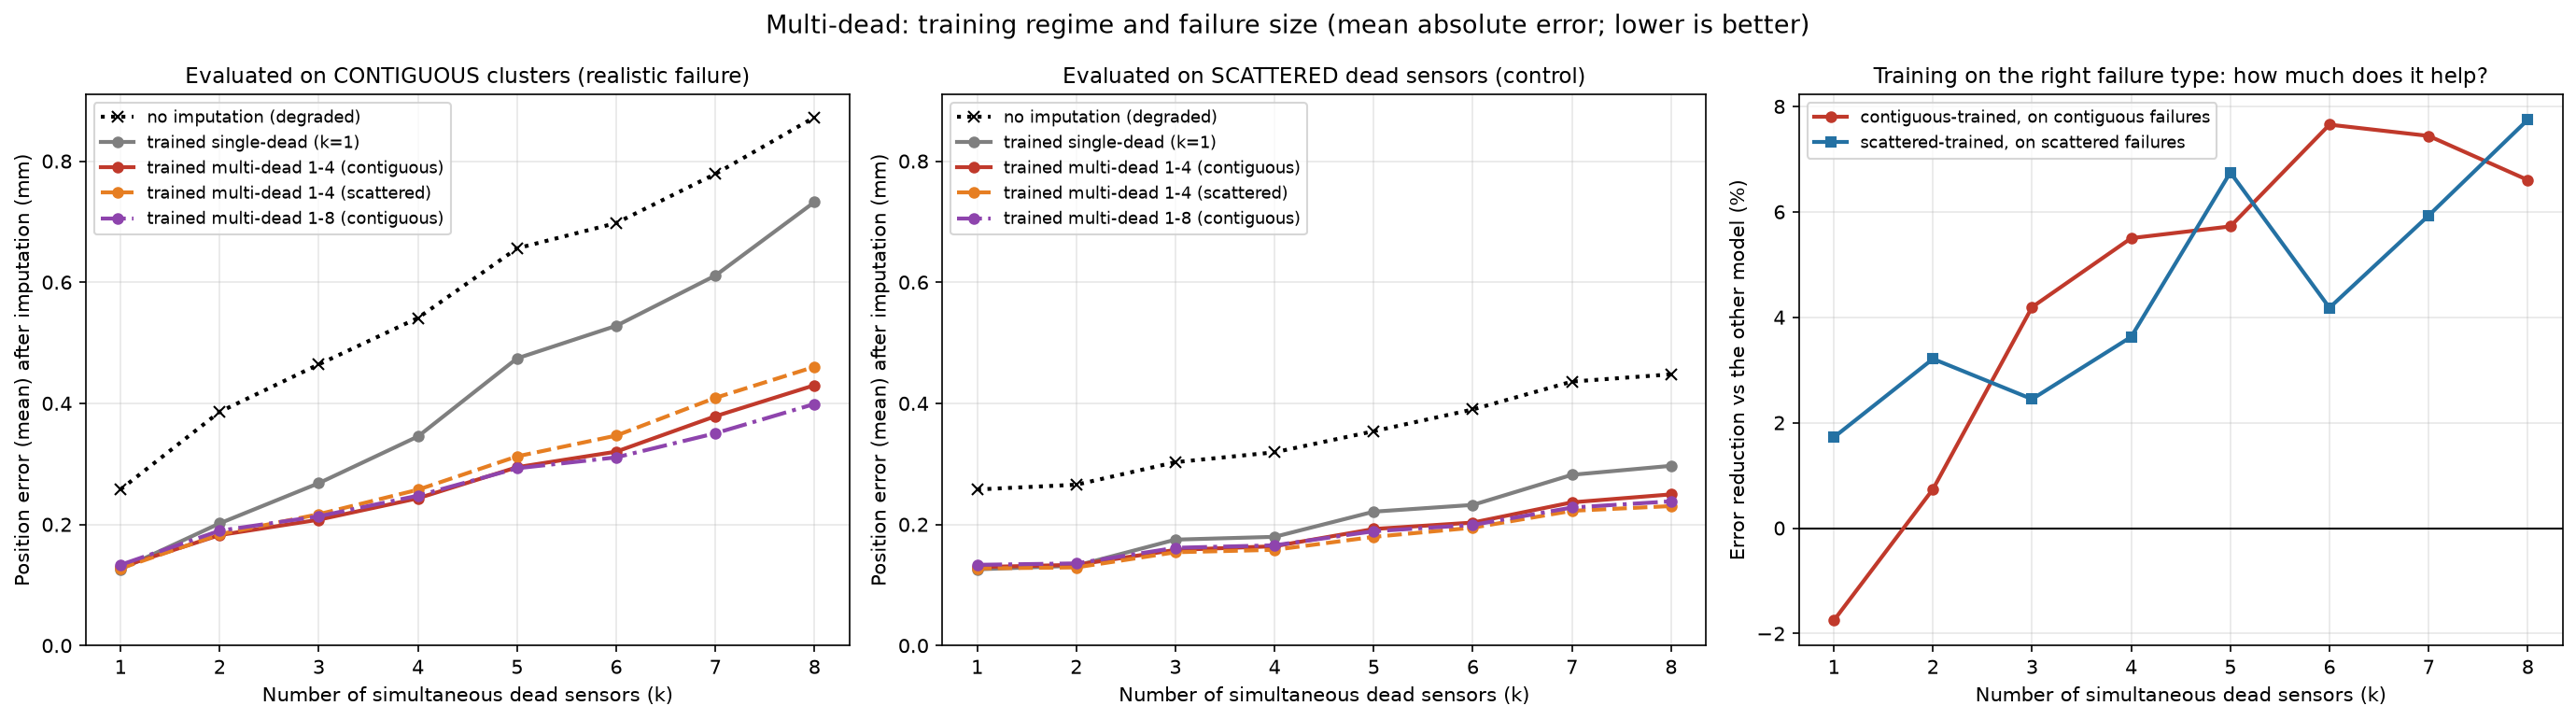
\includegraphics[width=\textwidth]{fig-multidead.png}
\caption{Error absoluto de posición tras la imputación en función del número de sensores averiados
simultáneamente, para los distintos regímenes de entrenamiento. El panel izquierdo corresponde a
fallos contiguos (caso realista) y el central a fallos dispersos (control); el panel derecho
cuantifica la ventaja de entrenar en el régimen que posteriormente se evalúa.}
\label{fig:multidead}
\end{figure}

Como referencia interpretativa, tras la imputación un fallo de ocho sensores contiguos ---el 13\,\%
del detector concentrado en una única región--- deja el módulo en una situación equivalente a la de
un fallo de dos sensores sin imputar, con un error muy inferior al paso entre sensores
(\SI{3.75}{\milli\metre}).

\subsection{Conservación del espectro de energía}
\label{subsec:res-espectro}

La Tabla~\ref{tab:res-espectro} presenta la recuperación espectral estratificada por zonas.

\begin{table}[htbp]
\centering
\caption{Recuperación espectral (\%) por zona del metahexágono y por sensor averiado,
modelo de referencia.}
\label{tab:res-espectro}
\begin{tabular}{lrrr}
\toprule
\textbf{Sensor averiado} & \textbf{Núcleo} & \textbf{Intermedia} & \textbf{Borde} \\
\midrule
$\mathrm{Ich}\,13$ (central) & 96.0 & 85.0 & 52.8 \\
$\mathrm{Ich}\,30$ (intermedio) & 78.6 & 88.7 & 91.7 \\
$\mathrm{Ich}\,32$ (mitad de lado) & 70.0 & 85.5 & 90.5 \\
$\mathrm{Ich}\,27$ (vértice) & 87.2 & 92.0 & 94.4 \\
$\mathrm{Ich}\,31$ (anómalo) & 84.3 & 70.4 & 76.5 \\
\midrule
\textbf{Media} & \textbf{83.2} & \textbf{84.3} & \textbf{81.2} \\
\bottomrule
\end{tabular}
\end{table}

La recuperación espectral se sitúa entre el 77\,\% y el 83\,\% según el sensor averiado, con un
residuo inferior al 0,5\,\% de la posición del fotopico. El resultado es \textbf{uniforme entre
zonas} (83,2 / 84,3 / 81,2), en contraste con la recuperación de posición, donde el borde sufre
apreciablemente más.

Esta disociación admite una interpretación física directa: la conservación de la energía requiere
únicamente acertar la \emph{magnitud} de la carga ausente, mientras que la reconstrucción de la
posición exige además que el \emph{reparto espacial} sea correcto. La estructura por sensor matiza
esta lectura: al enmascarar el sensor central y evaluar los eventos del borde, la recuperación cae
al 52,8\,\%, resultado esperable dado que dichos eventos apenas iluminan el centro del detector.

\subsection{Resolución espacial}
\label{subsec:res-resolucion}

La descomposición del error de posición en sesgo y dispersión arroja los resultados de la
Tabla~\ref{tab:res-resolucion}.

\begin{table}[htbp]
\centering
\caption{Descomposición del error de posición. Agregación macro sobre 61 canales.}
\label{tab:res-resolucion}
\begin{tabular}{lrrr}
\toprule
\textbf{Componente} & \textbf{Degradado} & \textbf{Imputado} & \textbf{Recuperación} \\
\midrule
Sesgo (mm) & 0.126 & 0.022 & 82.7\,\% \\
FWHM / dispersión (mm) & 0.166 & 0.085 & 48.8\,\% \\
\bottomrule
\end{tabular}
\end{table}

El contraste entre ambas componentes es informativo. El \textbf{sesgo se elimina casi por completo}
(82,7\,\%), lo que resulta esperable: el desplazamiento inducido por un canal ausente es sistemático
y por tanto predecible. La \textbf{dispersión se reduce únicamente a la mitad} (48,8\,\%), lo que
refleja el carácter irreducible de la incertidumbre evento a evento: el modelo puede estimar el
valor esperado de la carga ausente, pero no su realización concreta en un evento particular.

El análisis por canal revela que la recuperación mediana de la dispersión es del 51\,\%, con una cola
desfavorable: en dos o tres canales periféricos la mejora es marginal o incluso ligeramente negativa.

\subsection{Ensembles y descomposición sesgo-varianza}
\label{subsec:res-ensemble}

Ambos ensembles superan a la totalidad de sus miembros individuales
(Tabla~\ref{tab:res-ensemble}).

\begin{table}[htbp]
\centering
\caption{Rendimiento de los ensembles frente a la distribución de sus miembros.}
\label{tab:res-ensemble}
\begin{tabular}{lrrrr}
\toprule
\textbf{Configuración} & $\mathcal{R}_{\text{media}}$ & $\mathcal{R}_{p90}$ & \textbf{MAE} & $z$ ($\mathcal{R}_{\text{media}}$) \\
\midrule
Miembros (media $\pm$ desv.) & $52.32 \pm 0.35$ & $58.06 \pm 0.09$ & $0.6220 \pm 0.0026$ & --- \\
Ensemble homogéneo & 52.93 & 58.69 & \textbf{0.6110} & $+1.7$ \\
Ensemble heterogéneo & \textbf{53.21} & \textbf{58.73} & 0.6146 & $+2.5$ \\
\bottomrule
\end{tabular}
\end{table}

El ensemble heterogéneo supera al homogéneo en las métricas de posición, lo que establece que
\textbf{la diversidad arquitectónica aporta más que la diversidad de inicialización}. En el error de
carga, sin embargo, el homogéneo obtiene mejor resultado, lo que se atribuye a que el heterogéneo
incorpora miembros con peor rendimiento en dicha magnitud.

La lectura de mayor calado es la que corresponde a la descomposición sesgo-varianza. Si el error
estuviera dominado por la varianza entre entrenamientos, el promediado de tres modelos lo reduciría
en torno a un 40\,\%; si estuviera dominado por el límite de información, no lo alteraría. La
reducción observada es del \textbf{1,8\,\% en MAE}, de lo que se concluye que aproximadamente el
98\,\% del error es \textbf{irreducible} en el marco planteado.

\subsection{Estimación de incertidumbre}
\label{subsec:res-hetero}

El entrenamiento con la pérdida heterocedástica~\eqref{eq:nll} produjo una degradación severa:
$\mathcal{R}_{\text{media}} = 10.57$, MAE $= 1.31$ y error relativo del 63,2\,\%. La recuperación
mediana resultó \textbf{negativa} ($-18.16$), lo que indica que la imputación deja la posición en
peor situación que la ausencia de imputación.

La causa es un fallo conocido de la formulación: la pérdida~\eqref{eq:nll} permite al modelo reducir
el término cuadrático incrementando $\sigma$, pagando únicamente un coste logarítmico ---y por tanto
lineal en $\log\sigma$--- de modo que le resulta ventajoso sacrificar la precisión de $\mu$ a cambio
de declarar mayor incertidumbre. La corrección estándar consiste en un entrenamiento en dos fases,
con calentamiento bajo error cuadrático puro, o en el empleo de la formulación $\beta$-NLL. Se
documenta como línea de trabajo futuro.

\subsection{Cobertura del conjunto de entrenamiento}
\label{subsec:res-cobertura}

El experimento descrito en la Sección~\ref{subsec:exp-cobertura} arroja un resultado nítido y con
dos caras.

\begin{table}[htbp]
\centering
\caption{Efecto de entrenar con la totalidad de los módulos disponibles, a coste computacional
constante. Agregación macro sobre los 61 canales, \num{600000} eventos por fichero de test en ambos
casos.}
\label{tab:res-cobertura}
\small
\begin{tabular}{lrrr}
\toprule
\textbf{Magnitud} & \textbf{40 módulos} & \textbf{149 módulos} & \textbf{Diferencia} \\
\midrule
$\mathcal{R}_{p90}$ macro (\%) & 58.02 & 57.89 & $-0.13$ \\
$\mathcal{R}_{\text{media}}$ macro (\%) & 52.66 & 52.63 & $-0.02$ \\
$\mathcal{R}_{\text{mediana}}$ macro (\%) & 51.55 & 52.78 & $+1.23$ \\
MAE (ADC) & 0.620 & 0.616 & $-0.004$ \\
\midrule
Desviación entre canales (pts) & 4.49 & \textbf{3.77} & $-16\,\%$ \\
Recorrido entre canales (pts) & 25.2 & \textbf{15.4} & $-39\,\%$ \\
Peor canal (\%) & 38.6 & \textbf{47.9} & $\mathbf{+9.3}$ \\
Canal $\mathrm{Ich}\,31$ (\%) & 38.6 & \textbf{49.5} & $\mathbf{+11.0}$ \\
\bottomrule
\end{tabular}
\end{table}

\paragraph{En el rendimiento medio, ningún efecto.} La comparación pareada canal a canal arroja una
diferencia media de $-0.13$ puntos, con un estadístico $t = -0.49$ que no permite rechazar la
hipótesis nula, y solo 26 de los 61 canales mejoran, proporción indistinguible del azar. La
recuperación media queda en $52.63\,\%$, dentro de la banda de las réplicas
($52.32 \pm 0.35$). \textbf{El límite de rendimiento no procede de la cobertura del entrenamiento},
sino de la información físicamente disponible en los canales supervivientes. Este resultado
convierte en comprobación experimental directa lo que hasta ahora era una inferencia a partir de la
saturación de las distintas variantes arquitectónicas.

\paragraph{En la homogeneidad del detector, un efecto claro.} La dispersión entre canales se reduce
un $16\,\%$ y el recorrido entre el mejor y el peor sensor casi un $40\,\%$. El peor canal pasa de
$38.6\,\%$ a $47.9\,\%$, una mejora de $9.3$ puntos que, contrastada con la banda de las réplicas
para esa misma magnitud ($41.4 \pm 2.52$), corresponde a $z = +2.6$ y resulta por tanto
estadísticamente significativa.

\paragraph{Resolución del comportamiento anómalo de \texorpdfstring{$\mathrm{Ich}\,31$}{Ich 31}.}
Este canal, identificado sucesivamente como sensor defectuoso y como manifestación de la
variabilidad de ganancia entre módulos, mejora $11.0$ puntos al ampliar la cobertura. La
interpretación definitiva es que \textbf{los módulos de test en los que fallaba se encontraban fuera
del régimen estadístico representado en el entrenamiento}: no se trataba de un canal
intrínsecamente problemático, sino de una configuración de detector que el modelo nunca había
observado. Deja de constituir una anomalía del sensor para pasar a ser una manifestación medible de
la cobertura del conjunto de entrenamiento.

\paragraph{Conservación del espectro.} El efecto sobre la métrica energética apunta en la misma
dirección. La recuperación espectral media asciende de $82.9\,\%$ a $86.3\,\%$, y ---de nuevo lo más
relevante--- el peor caso mejora sustancialmente: la combinación más desfavorable, el canal central
evaluado sobre eventos de borde, pasa de $52.8\,\%$ a $65.8\,\%$. Nueve de las quince combinaciones
de canal y zona mejoran.

\paragraph{Resolución espacial y comparación con métodos clásicos.} Las dos magnitudes restantes se
mantienen sin cambios apreciables, lo que resulta coherente con la ausencia de efecto sobre el
rendimiento medio. La recuperación del emborronamiento mejora de forma marginal, de $48.8\,\%$ a
$49.5\,\%$, con una anchura a media altura residual prácticamente idéntica ($0.084$ frente a
$0.085$~mm) y una recuperación del sesgo equivalente ($82.6\,\%$ frente a $82.7\,\%$). La ventaja
sobre la regresión lineal, que sustenta la necesidad del aprendizaje profundo, se conserva en
$11.3$ puntos frente a los $11.5$ del modelo de referencia; la diferencia queda holgadamente dentro
de la variabilidad entre entrenamientos. Ninguno de los dos observables se ve por tanto perjudicado
por la ampliación de la cobertura.

\paragraph{Contrapartida: pérdida de robustez ante fallos múltiples.} La evaluación multi-dead
revela, sin embargo, un efecto de signo contrario que obliga a matizar la valoración. Ambos modelos
se entrenaron exclusivamente con un canal enmascarado, de modo que un fallo de dos o más sensores
constituye para ellos una situación no observada durante el entrenamiento. Con un único canal
averiado, el modelo de cobertura completa es superior, y de forma marcada en el peor caso
($45.9\,\%$ frente a $34.7\,\%$). Pero al aumentar el tamaño del fallo su rendimiento
\textbf{se desploma}: en agrupaciones contiguas de dos sensores la recuperación media cae a valores
negativos ---esto es, la imputación empeora la posición respecto a no imputar--- mientras que el
modelo de referencia se degrada de forma suave y conserva un $49.3\,\%$.

\begin{table}[htbp]
\centering
\caption{Recuperación media (\%) frente al tamaño del fallo, para dos modelos entrenados ambos con
un solo canal enmascarado. Valores negativos indican que la imputación desplaza la posición más de
lo que lo hace el propio fallo.}
\label{tab:res-cobertura-multidead}
\small
\begin{tabular}{lrrrr}
\toprule
\textbf{Modelo} & $k=1$ & $k=2$ & $k=3$ & $k=4$ \\
\midrule
\multicolumn{5}{l}{\emph{Agrupación contigua}} \\
\quad 40 módulos (referencia) & 51.39 & \textbf{49.28} & \textbf{44.21} & \textbf{37.59} \\
\quad 149 módulos & \textbf{51.64} & $-27.35$ & $-123.65$ & $-161.83$ \\
\midrule
\multicolumn{5}{l}{\emph{Fallo disperso}} \\
\quad 40 módulos (referencia) & 51.39 & \textbf{50.71} & \textbf{43.19} & \textbf{43.37} \\
\quad 149 módulos & \textbf{51.64} & 45.13 & 13.62 & $-3.96$ \\
\bottomrule
\end{tabular}
\end{table}

La interpretación más plausible es que el entrenamiento prolongado sobre un régimen de fallo único
---149 épocas frente a 40, con el punto de control seleccionado en la época 133--- produce una
función más ajustada a esa condición concreta y, por ello, más frágil fuera de la distribución de
entrenamiento. La cobertura completa mejora el caso para el que el modelo fue entrenado a costa de
su capacidad de extrapolación.

\paragraph{Implicación práctica.} Ampliar la cobertura no mejora el rendimiento promedio, pero
\textbf{homogeneiza la respuesta del detector sin coste computacional adicional}: eleva el peor
sensor nueve puntos y mejora la conservación del espectro. En un dispositivo real, donde la garantía
relevante es que ningún sensor se degrade de forma catastrófica, ese comportamiento resulta
preferible a una mejora marginal de la media. Ahora bien, la pérdida de robustez ante fallos
múltiples impide recomendar su adopción sin más: un modelo de producción con cobertura completa
debería entrenarse necesariamente en régimen multi-dead
(Sección~\ref{subsec:exp-multidead}), combinando ambas mejoras en lugar de intercambiarlas.

\subsection{Detección de canales defectuosos}
\label{subsec:res-bad}

La Tabla~\ref{tab:res-bad-roc} recoge la validación del estadístico de detección mediante inyección
de fallos con verdad conocida.

\begin{table}[htbp]
\centering
\caption{Validación del detector de canales defectuosos. Área bajo la curva ROC y tasas de
detección en el punto de operación.}
\label{tab:res-bad-roc}
\begin{tabular}{lrrr}
\toprule
\textbf{Severidad del fallo} & \textbf{AUC} & \textbf{TPR} ($Z=2.5$) & \textbf{FPR} \\
\midrule
100\,\% (canal muerto) & 1.000 & 1.000 & 0.009 \\
70\,\% & 0.998 & 0.952 & 0.009 \\
50\,\% & 0.973 & 0.422 & 0.009 \\
30\,\% & 0.868 & 0.091 & 0.009 \\
\bottomrule
\end{tabular}
\end{table}

El estadístico identifica los canales completamente inactivos con separación perfecta
($\mathrm{AUC} = 1.000$) y mantiene un rendimiento elevado para degradaciones severas. La tasa de
falsos positivos en los canales de borde resulta equivalente a la de los canales centrales, lo que
confirma que la normalización por canal resuelve efectivamente el problema del gradiente
estructural.

Las degradaciones moderadas, en cambio, no resultan separables en el punto de operación: si bien el
área bajo la curva indica que la información está presente, explotarla exigiría reducir el umbral y
asumir una tasa de falsos positivos considerablemente mayor.

\begin{figure}[htbp]
\centering
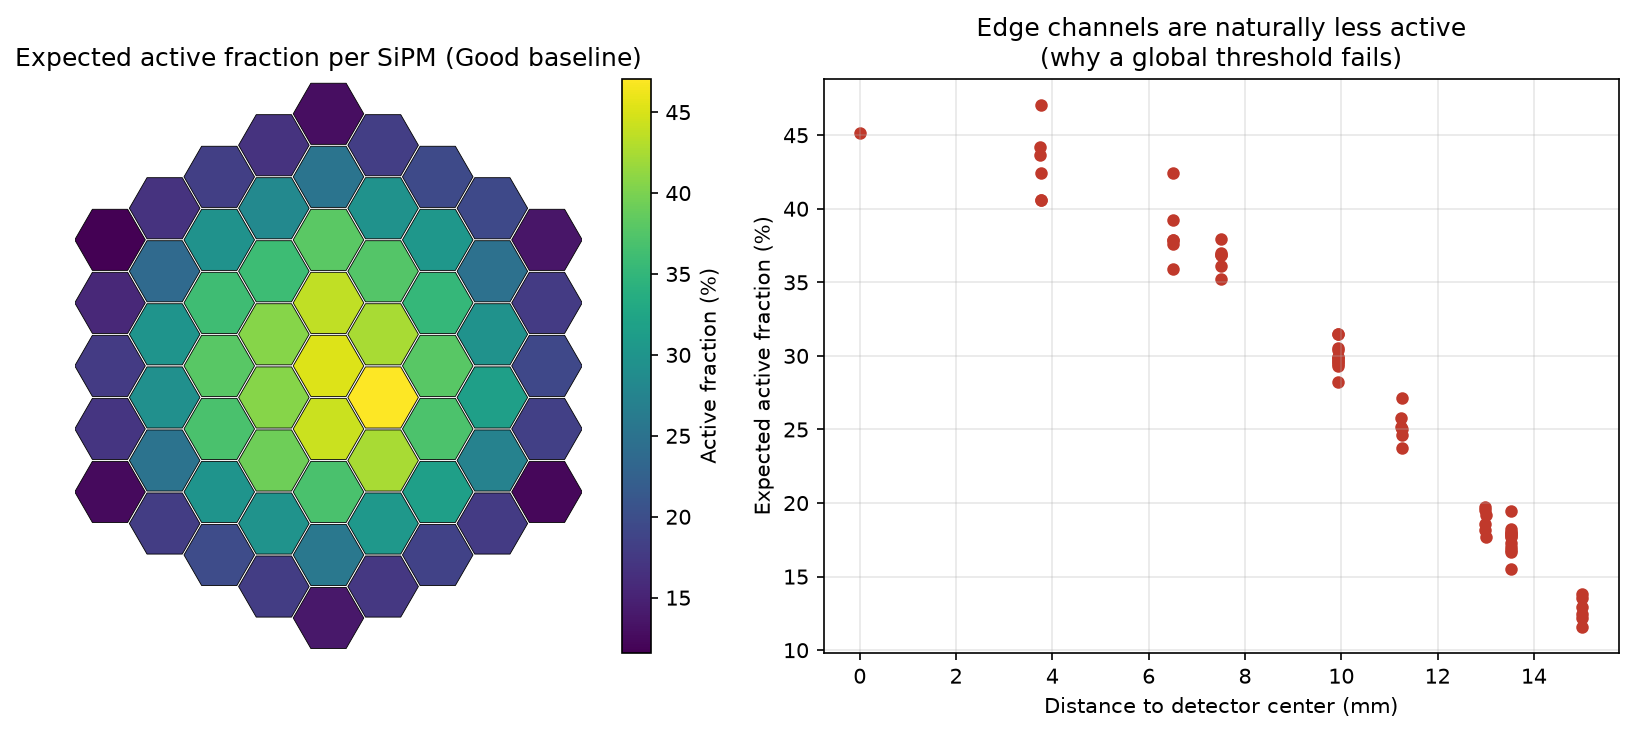
\includegraphics[width=0.95\textwidth]{fig-baseline-bad.png}
\caption{Actividad esperada por sensor en módulos sanos. Izquierda: mapa hexagonal del detector.
Derecha: dependencia con la distancia al centro, con una correlación de $-0.97$. Este gradiente
estructural es la razón por la que un umbral de detección global resulta inadecuado.}
\label{fig:baseline-bad}
\end{figure}

\begin{figure}[htbp]
\centering
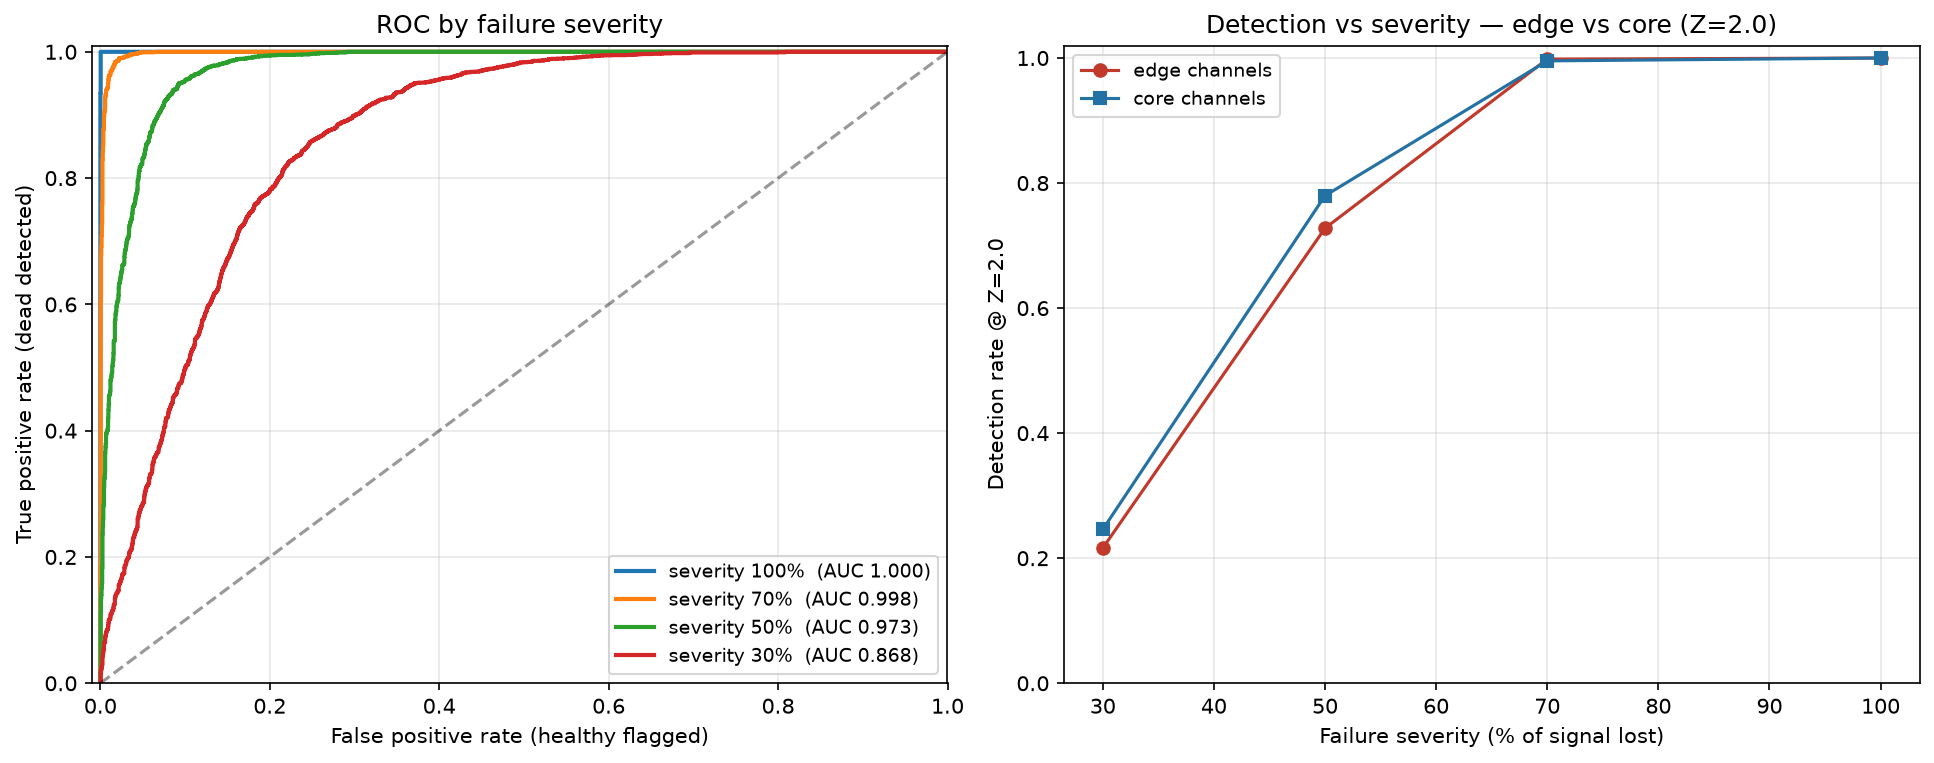
\includegraphics[width=0.95\textwidth]{fig-roc-bad.png}
\caption{Validación del estadístico de detección mediante inyección de fallos con verdad conocida.
Izquierda: curvas ROC para distintas severidades. Derecha: tasa de detección en el punto de
operación, desglosada entre canales de borde y centrales.}
\label{fig:roc-bad}
\end{figure}

Aplicado a los 62 módulos \textsc{Bad} con normalización por módulo y umbral $Z = 2.0$, el
procedimiento identifica canales defectuosos en \textbf{48} de los 62 módulos, marcando
\textbf{278} canales en total, y señala \textbf{12} módulos como globalmente desplazados.



\begin{figure}[htbp]
\centering
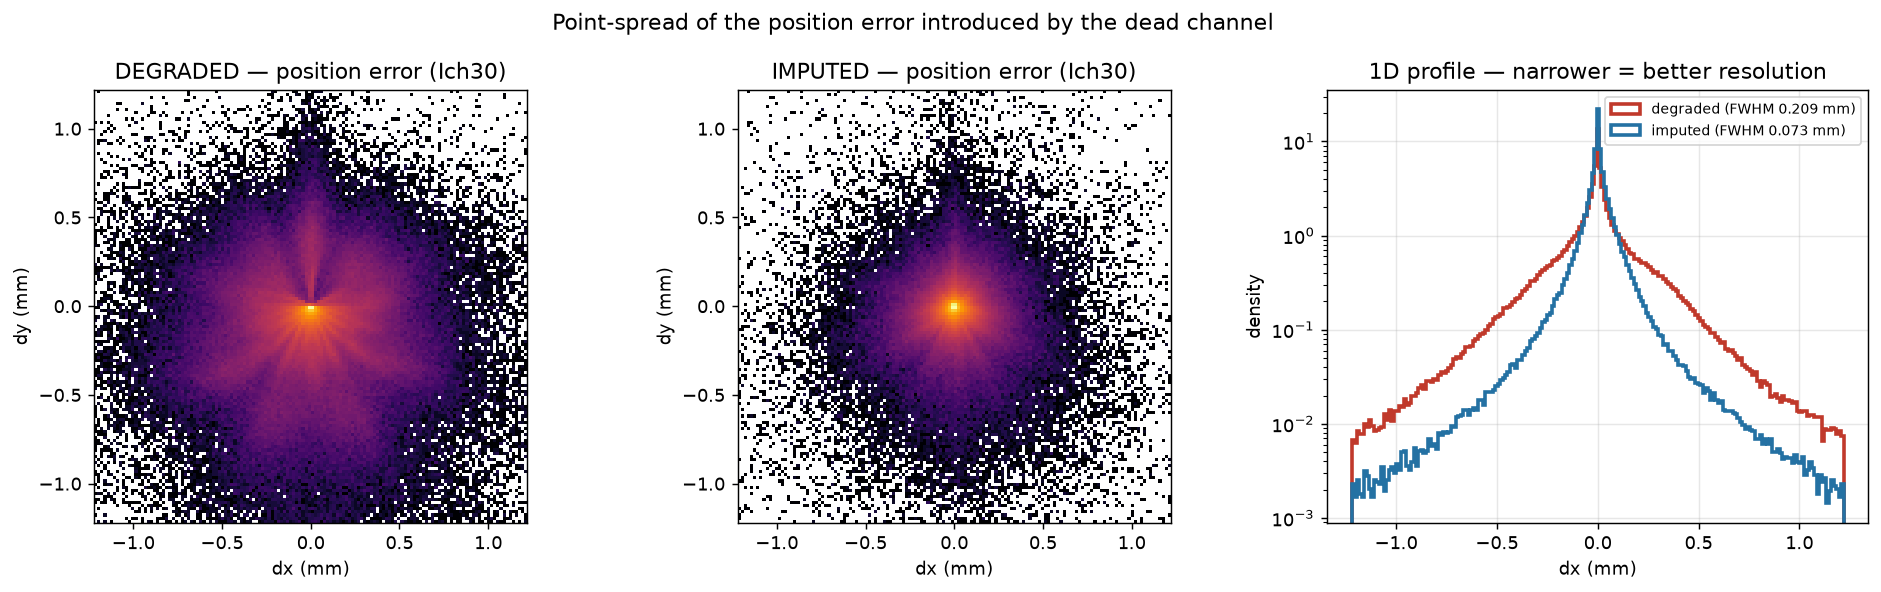
\includegraphics[width=0.95\textwidth]{fig-pointspread.png}
\caption{Distribución bidimensional del error de posición (\emph{point spread}) para el canal
$\mathrm{Ich}\,30$, antes y después de la imputación. La nube de la derecha es simultáneamente más
estrecha (menor dispersión) y está mejor centrada (menor sesgo) que la de la izquierda.}
\label{fig:pointspread}
\end{figure}

\begin{figure}[htbp]
\centering
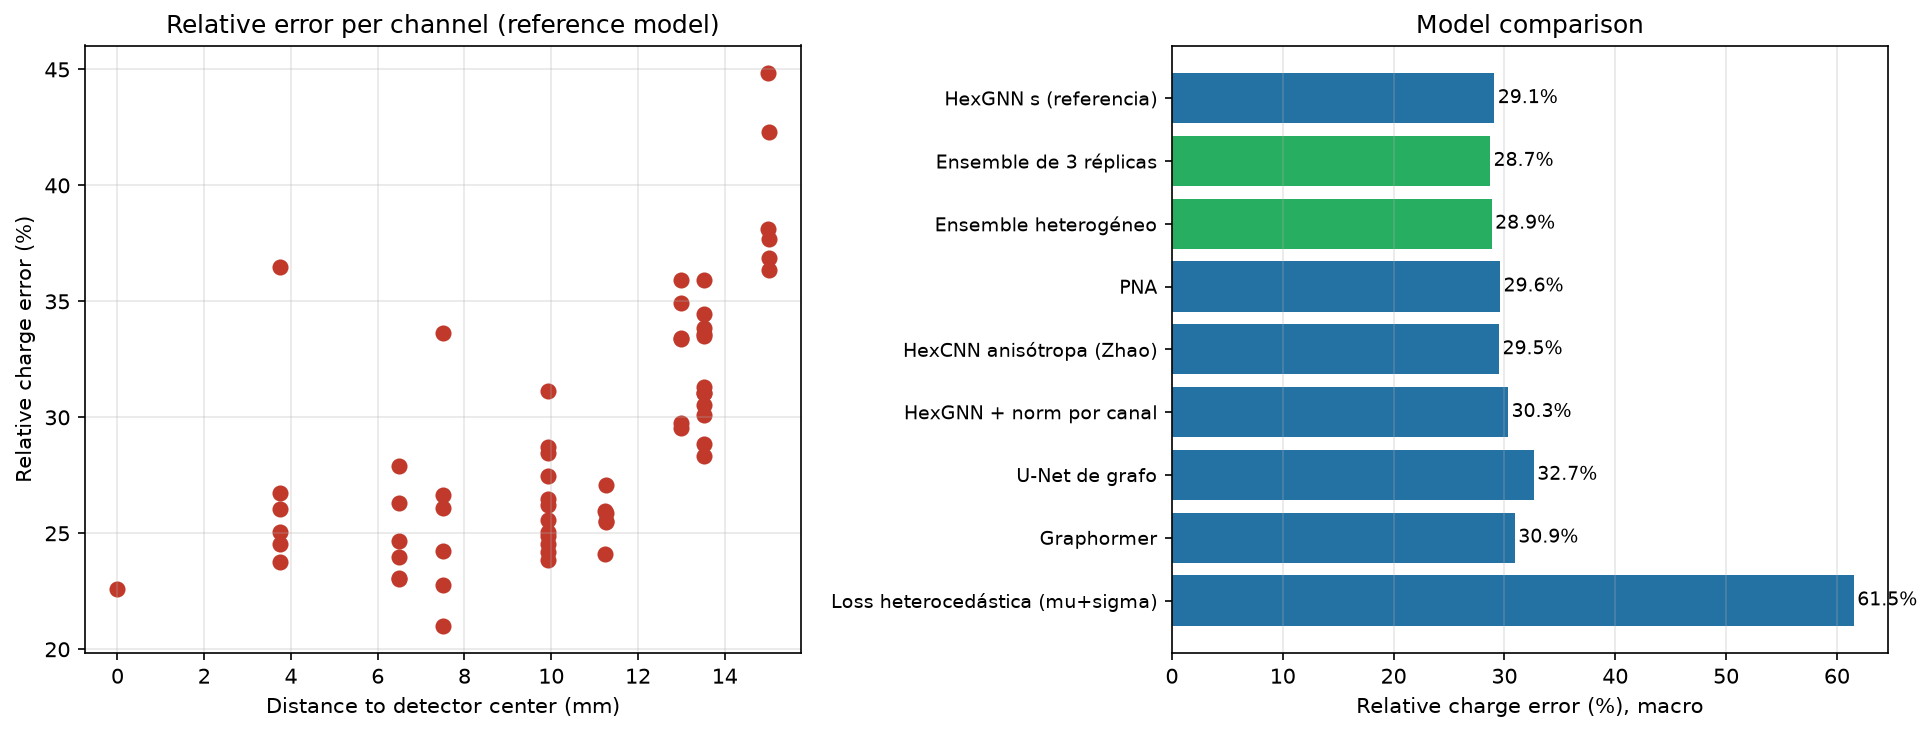
\includegraphics[width=0.95\textwidth]{fig-error-relativo.png}
\caption{Error relativo de carga. Izquierda: valor por canal frente a la distancia al centro del
detector, que evidencia el gradiente centro--borde. Derecha: comparación agregada entre las
configuraciones evaluadas.}
\label{fig:error-relativo}
\end{figure}

\section{Discusión}
\label{sec:discusion}

\subsection{Sobre la naturaleza del límite de rendimiento}

El conjunto de resultados converge de forma consistente hacia una conclusión: el rendimiento
alcanzado no está limitado por la arquitectura ni por la capacidad del modelo, sino por la
\textbf{información físicamente disponible} en los sensores operativos.

Esta conclusión se sustenta en cuatro evidencias independientes. En primer lugar, el incremento de
capacidad no mejora el rendimiento, e incluso lo degrada. En segundo lugar, diez variantes
arquitectónicas ---incluyendo transformadores, arquitecturas multiescala, agregadores múltiples y la
convolución hexagonal canónica--- no superan a la configuración de referencia. En tercer lugar, el
análisis por anillos demuestra que la información explotable se agota en el segundo anillo de
vecindad. Y en cuarto lugar, el ensemble ---que cancela la varianza entre entrenamientos--- recupera
únicamente un 1,8\,\% del error, lo que sitúa en torno al 98\,\% la fracción irreducible.

La descomposición del error de posición en sesgo y dispersión ofrece la interpretación física de
este límite. El sesgo, sistemático y por tanto predecible, se elimina casi por completo. La
dispersión, que corresponde a la incertidumbre sobre la realización concreta de la carga en cada
evento individual, solo se reduce a la mitad. Ninguna arquitectura puede eliminar esta segunda
componente, pues la información necesaria simplemente no está presente en los datos observados.

\subsection{Sobre la adecuación del diseño arquitectónico}

Los resultados permiten justificar el diseño adoptado desde tres perspectivas independientes.

La comparación con métodos clásicos establece que el aprendizaje profundo es \textbf{necesario}: la
red supera en 11,5 puntos a la regresión lineal. El análisis por anillos establece que la
información es \textbf{local}. Y la ablación del grafo establece que el prior geométrico es
\textbf{determinante}. En conjunto, estas tres evidencias caracterizan el modelo adecuado como uno
que sea simultáneamente local, no lineal e informado por la geometría del detector, que es
precisamente la descripción de la arquitectura propuesta.

El análisis de equivarianza añade una cuarta propiedad: la isotropía. La arquitectura respeta por
construcción la simetría $D_6$ del detector, propiedad que las variantes anisótropas rompen sin
obtener contrapartida, dado que el transporte de luz en el cristal es radialmente simétrico.

\subsection{Fortalezas del trabajo}

Cabe destacar como fortalezas metodológicas la definición de un marco de evaluación con significado
físico, que trasciende el error de reconstrucción y cuantifica el impacto sobre posición, energía y
resolución; el diseño diferencial emparejado para la evaluación espectral, que elimina la necesidad
de calibración previa; la estratificación mediante el metahexágono, físicamente motivada por la
geometría del absorbente; la inclusión sistemática de controles ---ablación del grafo, régimen
disperso, control de ruido en $k=1$, réplicas independientes--- que permiten atribuir causalmente los
efectos observados; y la cuantificación explícita de la variabilidad entre entrenamientos, que
proporciona el criterio para juzgar la significación de las comparaciones.

En el plano de los resultados, el hallazgo de que entrenar con fallos múltiples confiere robustez
sin coste alguno en el caso de un único canal tiene aplicabilidad práctica directa.

\subsection{Limitaciones}

\paragraph{Estadística de módulos reducida.} Conviene distinguir esta limitación de la cobertura del
entrenamiento tratada más abajo, con la que resulta fácil confundirla: aquella se refiere a
\emph{cuántos detectores ve el modelo} y afecta a lo que aprende; ésta se refiere a \emph{cuántos
detectores se emplean para medirlo} y afecta a la precisión de la métrica. Son independientes, y el
experimento de cobertura no resuelve la segunda.

La partición reserva únicamente cinco módulos para test. Aunque la estadística de eventos es holgada
---del orden de tres millones---, la de \emph{detectores} es pobre, de modo que las conclusiones
referidas a canales individuales pueden reflejar particularidades de esos cinco módulos concretos.
El caso del canal $\mathrm{Ich}\,31$ ilustra el problema: identificado inicialmente como canal
sistemáticamente anómalo, el análisis posterior reveló que su comportamiento en los módulos de
entrenamiento es normal y que la anomalía se concentra en dos módulos asignados a test; el
experimento de cobertura confirmó después que dichos módulos quedaban fuera del régimen estadístico
representado durante el entrenamiento.

La consecuencia metodológica es que las métricas agregadas carecen de una barra de error asociada al
\emph{efecto de módulo}: se dispone de la variabilidad entre entrenamientos
(Sección~\ref{subsec:res-replicas}), pero no de la variabilidad entre detectores. El procedimiento
descrito en el párrafo anterior ---evaluar sobre los 119 módulos no observados--- permite estimarla
sin reentrenar y se identifica como la comprobación pendiente de mayor valor.

\paragraph{Ausencia de validación cruzada.} No se ha realizado validación cruzada por módulos. La
razón no es el coste ---repetir el entrenamiento cinco veces es perfectamente asumible--- sino que
el número de hiperparámetros a ajustar es reducido y la selección del punto de control ya descansa
en un conjunto de validación independiente. Conviene, no obstante, precisar qué quedaría por
resolver: la validación cruzada no se necesitaría aquí para \emph{ajustar} nada, sino para
\textbf{acotar la sensibilidad de las métricas a qué cinco módulos concretos quedaron reservados
para test}, que es una cuestión distinta y sí pertinente.

Existe, además, una alternativa más económica y estadísticamente más potente que la validación
cruzada para esa pregunta concreta, derivada de la propia mecánica de rotación de ficheros. Puesto
que un modelo de 40 épocas solo llega a ver 40 de los 149 módulos de entrenamiento, los 109
restantes ---junto a los 5 de validación y los 5 de test--- constituyen \textbf{119 módulos que el
modelo no ha observado nunca}. Evaluar sobre ellos proporciona la dispersión entre detectores con
una estadística veinticuatro veces mayor que la del conjunto de test, y sin reentrenar. Es el
procedimiento recomendado para cerrar la limitación descrita en el párrafo siguiente.

\paragraph{Cobertura parcial del conjunto de entrenamiento.} El presupuesto de 40 épocas, combinado
con una rotación cíclica sobre la lista ordenada de ficheros, hace que el modelo utilice 40 de los
149 módulos disponibles, y que sean siempre los mismos. Como se detalla en la
Sección~\ref{subsec:carga-entrenamiento}, ese subconjunto resulta además más homogéneo que la
población completa. El experimento de la Sección~\ref{subsec:res-cobertura} demuestra que esta
limitación \textbf{no afecta al rendimiento medio} ---y por tanto no compromete ninguna de las
comparaciones entre modelos---, pero sí a la \emph{homogeneidad} entre canales: el protocolo de
producción subestima el peor caso en unos nueve puntos. Para trabajo posterior se recomienda adoptar
la cobertura completa, que no conlleva coste adicional.

\paragraph{Ausencia de calibración y filtrado en energía.} El conjunto incluye eventos Compton y de
fondo sin calibración de ganancia. Aunque el diseño diferencial cancela estos efectos en la
evaluación espectral, no puede descartarse que un conjunto calibrado y filtrado permitiera un
rendimiento superior.

\paragraph{Criterio de selección de modelo.} La métrica empleada para seleccionar el punto de
control no rastrea perfectamente el rendimiento en test, como se comprobó en el banco de pruebas.

\paragraph{Alcance del detector de canales defectuosos.} El estadístico desarrollado identifica de
forma fiable los canales inactivos, pero no separa las degradaciones moderadas de la variabilidad
normal, ni detecta canales con ganancia anómalamente elevada, dado que el estadístico es de una sola
cola. La distribución de puntuaciones en los módulos reales no presenta bimodalidad clara, lo que
indica que ``canal defectuoso'' no constituye una categoría con una firma estadística única sino un
conjunto heterogéneo de modos de fallo.

\paragraph{Ausencia de verdad de referencia en los módulos averiados.} La validación del detector se
apoya en fallos inyectados sobre módulos sanos, lo que garantiza una verdad conocida a costa de
evaluar un modo de fallo idealizado. En los módulos defectuosos reales no se dispone de anotación,
de modo que las detecciones no pueden contrastarse y el rendimiento medido no es directamente
extrapolable. La herramienta de etiquetado manual descrita en la Sección~\ref{subsec:exp-bad} se ha
desarrollado precisamente para levantar esta limitación; la anotación de los módulos y la medida del
acuerdo con el estadístico automático constituyen trabajo en curso.

\paragraph{Coste de inferencia del ensemble.} La mejor configuración identificada triplica el coste
de inferencia. Constituye por tanto una mejora en recursos y no en método, extremo que debe
explicitarse al reportar el resultado.

\subsection{Comparación entre aproximaciones}

La comparación entre familias arquitectónicas resulta ilustrativa. Los métodos sin estructura (MLP)
alcanzan recuperaciones del 48--51\,\%. Las arquitecturas basadas en paso de mensajes local se sitúan
en el rango 55--58\,\%. Las basadas en atención global obtienen 54--55\,\%, es decir, peor que las
locales pese a disponer de hasta cien veces más parámetros. La ordenación es coherente con la
naturaleza del problema: la estructura de grafo aporta, mientras que el contexto global no
únicamente no aporta sino que diluye la señal local relevante.

En cuanto a las estrategias de mejora ajenas a la arquitectura, se observa una asimetría notable:
mientras que ninguna modificación arquitectónica superó la referencia, el promediado de modelos sí
produjo una mejora estadísticamente significativa, aunque de magnitud modesta. Esto refuerza la
interpretación de que el margen de mejora disponible no reside en el diseño del modelo.


\section{Conclusiones preliminares}
\label{sec:conclusiones}

\subsection{Respuesta a los objetivos planteados}

\textbf{Sobre el diseño del modelo y el prior geométrico.} Se ha desarrollado una red neuronal de
grafos que explota la adyacencia física de los sensores, alcanzando una recuperación del error de
posición del 52--58\,\% con únicamente \num{38305} parámetros. La ablación del grafo establece de
forma concluyente que dicho prior es el elemento determinante del rendimiento: su eliminación reduce
la recuperación a la mitad.

\textbf{Sobre el marco de evaluación física.} Se ha desarrollado un conjunto de métricas que
cuantifican el impacto de la imputación sobre las tres magnitudes de interés. Los resultados indican
que el método recupera el 52--58\,\% del error de posición, el 77--83\,\% de la conservación del
espectro y el 48,8\,\% de la dispersión espacial, eliminando además el 82,7\,\% del sesgo
sistemático.

\textbf{Sobre la justificación del aprendizaje profundo.} La comparación con métodos clásicos
establece una ventaja de 11,5 puntos frente a la regresión lineal. El análisis por anillos precisa
el origen de dicha ventaja: no procede del acceso a información global ---que resulta irrelevante
más allá del segundo anillo--- sino de la capacidad de modelar relaciones no lineales.

\textbf{Sobre el límite del rendimiento.} El conjunto de evidencias establece que el rendimiento
está limitado por la información disponible y no por el modelo. La formulación de este resultado es
en sí misma una aportación: no se trata de que no se hayan encontrado arquitecturas mejores, sino de
que se ha caracterizado por qué la arquitectura adoptada es la adecuada.

\textbf{Sobre los fallos múltiples.} Entrenar con fallos múltiples contiguos reduce a la mitad el
error con ocho canales averiados, sin penalización alguna en el caso de un único canal, y
generalizando por encima del rango de entrenamiento. El régimen espacial del entrenamiento resulta
relevante, con una ventaja del 6--8\,\% frente a un nivel de ruido del 1,8\,\%.

\textbf{Sobre la detección de canales defectuosos.} Se ha desarrollado un estadístico que identifica
con separación perfecta los canales inactivos, resolviendo el problema del gradiente estructural
centro-borde. Su alcance queda limitado a los fallos severos.

\subsection{Contraste de las hipótesis planteadas}

De las hipótesis formuladas, se confirmaron la relativa al prior geométrico, la relativa a la
localidad de la información, la relativa al mayor daño de los fallos contiguos y la relativa al papel
del ensemble como estimador de la componente reducible del error.

Se refutaron, en cambio, las hipótesis relativas a la utilidad de las pérdidas physics-informed, al
beneficio de incorporar información direccional, a la ventaja de las arquitecturas de mayor
capacidad y a la conveniencia de la normalización por canal. Esta última merece comentario: la
hipótesis predecía una mejora en los canales periféricos, y el resultado fue una degradación
concentrada en los canales centrales. La explicación es que el estimador de posición pondera las
cargas cuadráticamente, de modo que los canales más brillantes dominan la magnitud de interés; la
pérdida cuadrática sin equalizar estaba, de forma no premeditada, alineada con esa ponderación, y
equalizar los canales rompe dicha alineación.

\subsection{Líneas de trabajo futuro}

Se identifican las siguientes líneas de continuación:

\begin{enumerate}
    \item \textbf{Estimación de incertidumbre con formulación corregida}, empleando entrenamiento en
    dos fases o la formulación $\beta$-NLL, con la finalidad de identificar y descartar los eventos
    cuya imputación resulte poco fiable.

    \item \textbf{Ampliación del estadístico de detección} mediante observables sensibles a la forma
    de la distribución de carga y con formulación de dos colas, que permitiría abordar los modos de
    fallo actualmente no cubiertos.

    \item \textbf{Combinación de cobertura completa y entrenamiento multi-canal.} Los resultados de
    la Sección~\ref{subsec:res-cobertura} muestran que ampliar la cobertura de módulos mejora la
    homogeneidad entre sensores y la conservación del espectro, pero degrada la extrapolación a
    fallos múltiples, mientras que el entrenamiento en régimen multi-canal
    (Sección~\ref{subsec:res-multidead}) proporciona precisamente esa robustez sin coste apreciable
    en el caso de fallo único. Al actuar sobre aspectos independientes del procedimiento, ambas
    intervenciones son en principio acumulables, y su combinación constituye la vía más directa
    hacia un modelo de producción que reúna las dos propiedades.

    \item \textbf{Anotación manual completa de los módulos averiados} con la herramienta descrita en
    la Sección~\ref{subsec:exp-bad}, que proporcionaría la verdad de referencia necesaria para medir
    el acuerdo entre el criterio experto y el estadístico automático sobre datos reales, y no
    únicamente sobre fallos inyectados.

    \item \textbf{Validación cruzada por módulos}, que permitiría acotar la sensibilidad de los
    resultados a la partición concreta y robustecer las conclusiones referidas a canales
    individuales.

    \item \textbf{Incorporación de la calibración en energía} y del filtrado correspondiente, con el
    fin de determinar si un conjunto de datos calibrado permite superar el límite observado.

    \item \textbf{Extensión a la corrección de canales anómalos}, generalizando el planteamiento
    desde la imputación de canales ausentes a la corrección de canales con respuesta alterada.

    \item \textbf{Evaluación del impacto sobre la imagen reconstruida}, cerrando la cadena desde la
    recuperación del módulo individual hasta la calidad de la imagen tomográfica final.
\end{enumerate}

% =====================================================================
%  MARCADORES PENDIENTES DE COMPLETAR
% =====================================================================
% TODO(1): Especificar el modelo concreto de SiPM, sus dimensiones activas y el
%          espesor del cristal LYSO. Esta información debe obtenerse de la
%          documentación del sistema experimental o del equipo del laboratorio.
% TODO(2): Detallar la actividad de la fuente de 22Na, la geometría de irradiación
%          y la duración de las adquisiciones.
% TODO(3): Especificar el modelo de ASIC empleado y el valor del umbral de
%          discriminación aplicado.
% TODO(5): Incluir las referencias bibliográficas correspondientes a: GraphSAGE
%          (Hamilton et al., 2017), PNA (Corso et al., 2020), Graphormer (Ying
%          et al., 2021), Graph U-Net (Gao y Ji, 2019), convolución hexagonal
%          (Zhao et al., 2021), beta-NLL (Seitzer et al., 2022), AdamW (Loshchilov
%          y Hutter, 2019) y modified z-score (Iglewicz y Hoaglin, 1993).
% TODO(6): Generar y enlazar las figuras marcadas como [FIGURA SUGERIDA].

\end{document}
.
% =====================================================================

\documentclass[11pt,a4paper]{report}

% ── Codificación e idioma ────────────────────────────────────────────
\usepackage[utf8]{inputenc}
\usepackage[T1]{fontenc}
\usepackage[spanish,es-tabla]{babel}
\usepackage{lmodern}
\usepackage{microtype}

% ── Matemáticas ──────────────────────────────────────────────────────
\usepackage{amsmath}
\usepackage{amssymb}

% ── Tablas y figuras ─────────────────────────────────────────────────
\usepackage{booktabs}
\usepackage{graphicx}
\usepackage{multirow}
\usepackage{siunitx}
\usepackage[font=small,labelfont=bf]{caption}
\usepackage{float}

% ── Formato de página ────────────────────────────────────────────────
\usepackage[a4paper,margin=2.7cm]{geometry}
\usepackage{setspace}
\onehalfspacing
\usepackage{fancyhdr}
\pagestyle{fancy}
\fancyhf{}
\fancyhead[L]{\small\nouppercase{\leftmark}}
\fancyhead[R]{\small\thepage}
\renewcommand{\headrulewidth}{0.4pt}

% ── Enlaces y referencias cruzadas ───────────────────────────────────
\usepackage[colorlinks=true,linkcolor=black,citecolor=black,urlcolor=blue]{hyperref}

% ── Configuración de siunitx (separador decimal español) ─────────────
\sisetup{
  output-decimal-marker = {.},
  group-separator = {\,},
  group-minimum-digits = 4,
  detect-weight = true,
  detect-family = true
}

% ── Ruta de las figuras ──────────────────────────────────────────────
\graphicspath{{figuras/}}

% =====================================================================

\title{%
    \vspace*{2cm}
    {\Huge\bfseries Materiales y métodos}\\[1.2cm]
    {\Large Imputación auto-supervisada de canales SiPM defectuosos\\
     en un detector PET de cristal monolítico hexagonal}\\[0.8cm]
    {\large Trabajo Fin de Máster}
}
\author{Miguel Escudero}
\date{\today}

\begin{document}

\maketitle
\tableofcontents
\listoftables
\listoffigures
\cleardoublepage

\chapter{Materiales y métodos}
\label{cap:materiales-metodos}

\section{Descripción del problema}
\label{sec:descripcion-problema}

\subsection{Contexto: detectores PET de cristal monolítico}
\label{subsec:contexto-pet}

La tomografía por emisión de positrones (PET) reconstruye la distribución espacial de un
radiotrazador emisor de positrones a partir de la detección en coincidencia de los dos fotones
de aniquilación de \SI{511}{\kilo\electronvolt} emitidos en direcciones opuestas. La calidad de
la imagen reconstruida depende de forma crítica de la precisión con que cada módulo detector
determina el punto de interacción del fotón incidente dentro del cristal centelleador.

Históricamente, los detectores PET han empleado matrices de cristales segmentados (\emph{pixelated
arrays}), en los que la posición de interacción se identifica con el cristal individual que
centellea. Esta aproximación desacopla la resolución espacial del proceso de reconstrucción, pero
impone un límite duro: la resolución no puede ser mejor que el tamaño del píxel, y la fracción de
material inactivo entre cristales (el \emph{dead space} de los separadores reflectantes) reduce la
sensibilidad efectiva del sistema.

Los detectores de \textbf{cristal monolítico} constituyen la alternativa que motiva este trabajo.
En ellos, un único bloque continuo de material centelleador ---en el sistema estudiado, un cristal
de ortosilicato de lutecio e itrio dopado con cerio (LYSO)--- se acopla ópticamente a una matriz
de fotomultiplicadores de silicio (SiPM). Cuando un fotón gamma interacciona en el interior del
cristal, la luz de centelleo se propaga isótropamente desde el punto de interacción y genera una
distribución de intensidad continua sobre el plano de sensores. La posición de interacción no se
lee directamente, sino que se \emph{estima} a partir del patrón de reparto de luz entre los
sensores. Esta estrategia elimina el material inactivo entre cristales, mejora la sensibilidad,
y permite en principio una resolución espacial superior al paso entre sensores, además de habilitar
la estimación de la profundidad de interacción (DOI). El precio a pagar es que la reconstrucción
de la posición deja de ser trivial y pasa a depender de un algoritmo de estimación.

El estimador clásico, y el empleado como referencia en este trabajo, es el
\textbf{centro de gravedad ponderado} (\emph{Anger logic}). Dadas las cargas $\{R_c\}_{c=1}^{N}$
registradas por los $N$ sensores situados en posiciones $\{(x_c, y_c)\}$, la posición estimada del
evento se calcula como

\begin{equation}
    \hat{x} = \frac{\sum_{c=1}^{N} R_c^{2}\, x_c}{\sum_{c=1}^{N} R_c^{2}},
    \qquad
    \hat{y} = \frac{\sum_{c=1}^{N} R_c^{2}\, y_c}{\sum_{c=1}^{N} R_c^{2}}.
    \label{eq:centroide}
\end{equation}

El exponente cuadrático sobre las cargas ---en lugar del centro de masas lineal--- concentra el
peso del estimador en los sensores más iluminados, lo que reduce la contribución de las colas de la
distribución de luz y mejora empíricamente la resolución en el interior del cristal. Nótese que la
expresión~\eqref{eq:centroide} es invariante frente a un reescalado global de las cargas
($R_c \rightarrow \alpha R_c$), propiedad que se explotará más adelante al normalizar los eventos.

La representación estándar de la respuesta de un detector monolítico es el \textbf{flood map}: el
histograma bidimensional de las posiciones $(\hat{x}, \hat{y})$ reconstruidas para un gran número de
eventos bajo irradiación uniforme. En un detector sano, el flood map presenta una estructura
característica que refleja tanto la geometría del cristal como la respuesta óptica del conjunto.

\subsection{El problema: canales SiPM defectuosos}
\label{subsec:problema-canales}

La expresión~\eqref{eq:centroide} pone de manifiesto la vulnerabilidad fundamental de los
detectores monolíticos: \textbf{la posición reconstruida depende simultáneamente de todos los
sensores}. Si un canal SiPM deja de funcionar ---y su carga registrada pasa a ser idénticamente
nula--- el numerador y el denominador del estimador se ven alterados de forma sistemática, y la
posición reconstruida se desplaza en dirección opuesta al sensor averiado. El efecto no es un ruido
aleatorio que se promedie a lo largo de la adquisición, sino un \textbf{sesgo estructural} que
distorsiona el flood map completo del módulo.

En un detector segmentado, la avería de un canal implica simplemente la pérdida del cristal
correspondiente: se degrada la sensibilidad, pero la posición de los eventos restantes no se ve
afectada. En un detector monolítico, en cambio, un único canal defectuoso contamina la
reconstrucción de \emph{todos} los eventos cuya distribución de luz alcanzaba a ese sensor. La
consecuencia práctica es que el módulo completo debe descartarse, sustituirse o recalibrarse, con el
coste asociado en tiempo de máquina y en disponibilidad del escáner.

Los modos de fallo observados en el sistema estudiado son heterogéneos. Se han identificado módulos
con un único canal completamente inactivo, módulos con bloques enteros del perímetro apagados
---compatibles con fallos de conexión en serie, sombras mecánicas o efectos térmicos localizados---
y canales que, sin estar muertos, presentan una ganancia anómala. Esta variedad condiciona el diseño
experimental descrito en la Sección~\ref{sec:experimentos}.

\subsection{Planteamiento como problema de imputación auto-supervisada}
\label{subsec:planteamiento}

La propuesta de este trabajo consiste en abordar la avería de un canal como un
\textbf{problema de imputación de datos faltantes}: dado el vector de cargas de los sensores
operativos, estimar la carga que \emph{habría} registrado el sensor averiado, de modo que la
expresión~\eqref{eq:centroide} pueda evaluarse sobre un vector completo y la posición reconstruida
recupere su valor correcto.

Formalmente, sea $\mathbf{R} = (R_1, \dots, R_N) \in \mathbb{R}_{\geq 0}^{N}$ el vector de cargas de
un evento y sea $\mathcal{D} \subset \{1,\dots,N\}$ el conjunto de canales averiados. Se busca una
función $f_\theta$ parametrizada por $\theta$ tal que

\begin{equation}
    \hat{R}_c = f_\theta\!\left(\mathbf{R}_{\setminus \mathcal{D}}, \mathcal{D}\right)_c
    \approx R_c
    \qquad \forall\, c \in \mathcal{D},
    \label{eq:problema-imputacion}
\end{equation}

donde $\mathbf{R}_{\setminus \mathcal{D}}$ denota el vector de cargas con los canales averiados
puestos a cero. La aproximación se juzga no por el error en la carga en sí, sino por su efecto sobre
la magnitud físicamente relevante: la posición reconstruida mediante~\eqref{eq:centroide}.

El aspecto metodológicamente central del planteamiento es su carácter
\textbf{auto-supervisado}. No se dispone de pares (entrada degradada, salida correcta) en los
módulos averiados reales, puesto que la carga verdadera del canal muerto es por definición
inobservable. Sin embargo, sí se dispone de un gran número de módulos \emph{sanos}, en los que es
posible \textbf{simular} la avería: se selecciona un canal, se fuerza su carga a cero, y se emplea
su valor original como etiqueta de supervisión. La supervisión, por tanto, se genera a partir de los
propios datos sin necesidad de anotación externa, lo que sitúa el enfoque en el paradigma del
aprendizaje auto-supervisado por enmascaramiento, análogo conceptualmente a los modelos de lenguaje
enmascarado o a los \emph{masked autoencoders} en visión por computador.

\paragraph{Fundamento físico de la imputabilidad.} Que el problema admita solución no resulta
evidente a priori y conviene justificarlo antes de describir el método. La luz de centelleo
generada por una interacción no se deposita sobre un único fotosensor: el cristal monolítico
reparte el destello sobre una vecindad de SiPM, de modo que la carga de cada canal constituye una
muestra local de una distribución de luz continua y extensa. La información asociada a un sensor
concreto se encuentra, por tanto, \textbf{parcialmente contenida en los sensores que lo rodean}, y
es precisamente esa redundancia la que hace posible reconstruir su valor. El tratamiento
superficial del cristal acota lateralmente la propagación de la luz y confina el destello a una
región de tamaño finito, lo que explica que la redundancia tenga carácter \emph{local}: los vecinos
inmediatos concentran la mayor parte de la información recuperable, mientras que los sensores
alejados apenas aportan. Esta observación anticipa un resultado experimental que se presenta más
adelante (Sección~\ref{subsec:res-anillos}) y motiva el diseño de una arquitectura basada en
vecindades.

Conviene precisar además en qué consiste realmente la tarea que aprende el modelo, pues la
formulación ingenua induce a error. La red no aprende una regla del tipo «si un sensor está apagado,
sustitúyase su valor»: aprende a evaluar si la carga observada en un canal resulta
\textbf{coherente con la distribución de luz que describen los canales restantes}. Para el cálculo
del centroide, por otra parte, no es el valor absoluto de carga de un SiPM lo determinante, sino el
modo en que la luz se reparte entre varios de ellos, lo que refuerza la decisión de normalizar por
evento discutida en la Sección~\ref{subsec:normalizacion}. Esta formulación tiene una consecuencia
práctica inmediata sobre el diseño del muestreo: el modelo debe aprender tanto a corregir cuando la
degradación altera la distribución de luz como a \textbf{abstenerse de corregir} cuando no la
altera, lo que fundamenta físicamente el esquema de balanceo descrito en la
Sección~\ref{subsec:generacion-muestras}.

\subsection{Objetivos}
\label{subsec:objetivos}

El objetivo general del trabajo es \emph{desarrollar y validar un método de imputación de canales
SiPM defectuosos en un detector PET de cristal monolítico que permita recuperar la calidad de
reconstrucción del módulo sin necesidad de sustituir el hardware}. Este objetivo se concreta en los
siguientes objetivos específicos:

\begin{enumerate}
    \item \textbf{Diseñar un modelo de imputación} que explote la estructura geométrica del
    detector, y caracterizar en qué medida dicho prior geométrico contribuye al rendimiento.

    \item \textbf{Establecer el marco de evaluación física} adecuado, que no se limite al error de
    reconstrucción de la carga sino que cuantifique el impacto sobre las magnitudes de interés en
    PET: la posición reconstruida, el espectro de energía y la resolución espacial.

    \item \textbf{Determinar si el aprendizaje profundo está justificado} frente a alternativas
    clásicas de menor complejidad, mediante una comparación rigurosa con métodos de interpolación
    y regresión lineal.

    \item \textbf{Explorar el espacio de arquitecturas} para establecer si el rendimiento obtenido
    está limitado por la capacidad del modelo o por la información físicamente disponible.

    \item \textbf{Extender el método al caso de múltiples canales averiados simultáneamente},
    con especial atención a la configuración físicamente realista de fallos contiguos.

    \item \textbf{Desarrollar un procedimiento de detección} de canales defectuosos que permita
    aplicar el método sobre módulos reales no etiquetados.
\end{enumerate}


\section{Materiales}
\label{sec:materiales}

\subsection{Sistema detector}
\label{subsec:sistema-detector}

El sistema experimental del que proceden los datos consiste en módulos detectores basados en un
cristal centelleador monolítico de LYSO de geometría hexagonal, acoplado a una matriz de SiPM
dispuestos en una retícula hexagonal. La lectura se realiza mediante un circuito integrado de
aplicación específica (ASIC) que digitaliza la carga integrada por cada canal y aplica un umbral de
discriminación para suprimir el ruido electrónico.

La matriz de fotosensores consta de \textbf{64 canales} de lectura, de los cuales \textbf{61 se
encuentran físicamente instrumentados}; los canales con identificadores $\mathrm{Ich} \in
\{1, 16, 18\}$ no disponen de SiPM asociado y se excluyen sistemáticamente del análisis. En lo
sucesivo se emplea una indexación densa $i \in \{0, \dots, 60\}$ sobre los canales activos, junto
con las tablas de conversión correspondientes al identificador físico $\mathrm{Ich}$.

Las posiciones físicas de los 61 sensores se obtienen del fichero de configuración
\texttt{psipm.tsv}. La caracterización geométrica derivada de dichas posiciones se resume en la
Tabla~\ref{tab:geometria-detector}. Cabe destacar que el paso entre sensores vecinos
(\emph{pitch}) es de \SI{3.75}{\milli\metre}, valor que constituye la escala natural de referencia
para interpretar los errores de posición reportados en la Sección~\ref{sec:resultados}.

\begin{table}[htbp]
\centering
\caption{Caracterización geométrica del módulo detector, obtenida de las posiciones físicas
de los sensores.}
\label{tab:geometria-detector}
\begin{tabular}{lc}
\toprule
\textbf{Magnitud} & \textbf{Valor} \\
\midrule
Canales de lectura totales & 64 \\
Canales instrumentados (activos) & 61 \\
Canales inactivos ($\mathrm{Ich}$) & 1, 16, 18 \\
Paso entre sensores vecinos (\emph{pitch}) & \SI{3.75}{\milli\metre} \\
Extensión en $x$ & $[-13.0,\ 13.0]$~mm \\
Extensión en $y$ & $[-15.0,\ 15.0]$~mm \\
Radio máximo desde el centro & \SI{15.01}{\milli\metre} \\
Geometría de la retícula & Hexagonal (hexágono de lado 5) \\
\bottomrule
\end{tabular}
\end{table}

Un aspecto físico determinante para la interpretación de los resultados es la presencia de un
\textbf{adhesivo absorbente (negro) en las caras laterales del cristal}. Su función es suprimir las
reflexiones en los bordes, que de otro modo degradarían la estimación de posición, pero tiene como
efecto colateral que los eventos que interaccionan cerca del perímetro pierden una fracción
significativa de la luz de centelleo. Este hecho, confirmado por el análisis de los datos, se
traduce en dos observaciones recurrentes a lo largo del trabajo: los sensores del borde registran
sistemáticamente menos carga que los centrales, y el fotopico de energía se desplaza hacia energías
menores en las regiones periféricas del cristal.

\begin{figure}[htbp]
\centering
% \includegraphics[width=0.6\textwidth]{figuras/geometria_detector.pdf}
\caption{\textbf{[FIGURA SUGERIDA]} Disposición de los 61 SiPM activos sobre el plano del detector,
con la retícula hexagonal y la numeración $\mathrm{Ich}$ de cada canal. Se recomienda superponer el
contorno del cristal y señalar la posición del adhesivo absorbente en las caras laterales.}
\label{fig:geometria-detector}
\end{figure}

\subsection{Entorno software}
\label{subsec:entorno-software}

La totalidad del desarrollo se ha realizado en Python sobre un entorno gestionado con
\texttt{conda}. La Tabla~\ref{tab:entorno-software} recoge las versiones exactas de los componentes
empleados, información necesaria para garantizar la reproducibilidad de los experimentos.

\begin{table}[htbp]
\centering
\caption{Entorno software y hardware empleado en el desarrollo y la experimentación.}
\label{tab:entorno-software}
\begin{tabular}{lll}
\toprule
\textbf{Componente} & \textbf{Versión} & \textbf{Función en el trabajo} \\
\midrule
Python & 3.11.15 & Lenguaje de implementación \\
PyTorch & 2.5.1+cu121 & Definición y entrenamiento de los modelos \\
CUDA & 12.1 & Aceleración por GPU \\
NumPy & 2.4.4 & Álgebra y manipulación de arrays \\
SciPy & 1.17.1 & \texttt{cKDTree}, \texttt{ConvexHull}, distancia de Wasserstein \\
Matplotlib & 3.11.0 & Generación de figuras \\
openpyxl & 3.1.5 & Exportación de tablas de métricas \\
Weights \& Biases & 0.28.0 & Registro y trazabilidad de experimentos \\
\midrule
GPU & NVIDIA GTX 1660 SUPER & Entrenamiento e inferencia \\
Sistema operativo & Windows 11 & Entorno de ejecución \\
\bottomrule
\end{tabular}
\end{table}

La elección de PyTorch como \emph{framework} responde a la necesidad de implementar operadores de
paso de mensajes sobre un grafo con topología fija y no estándar. Aunque existen bibliotecas
especializadas en redes de grafos (\texttt{PyTorch Geometric}, \texttt{DGL}), se optó
deliberadamente por una implementación directa con tensores densos. Esta decisión se justifica por
tres motivos: el grafo del detector es pequeño ($N = 61$ nodos) y \emph{fijo}, lo que hace que la
indexación densa sea más eficiente que las estructuras dispersas generales; se elimina una
dependencia externa cuyo ciclo de versiones es sensible a la de PyTorch; y, sobre todo, se mantiene
control explícito sobre la operación de agregación, aspecto que resulta central en los experimentos
de la Sección~\ref{sec:experimentos}.

\subsection{Herramientas de desarrollo y trazabilidad}
\label{subsec:herramientas}

El control de versiones del código se ha realizado con Git, sobre un repositorio alojado en GitHub.
El seguimiento de los experimentos de entrenamiento y evaluación se ha llevado a cabo con
Weights~\&~Biases, registrando de forma sistemática los hiperparámetros, las curvas de entrenamiento
y las figuras resultantes de cada evaluación. Los procesos de entrenamiento y evaluación se
registran como ejecuciones diferenciadas mediante el campo \texttt{job\_type}, lo que permite
trazar qué evaluación corresponde a qué modelo.

Adicionalmente, se ha mantenido un cuaderno de laboratorio en formato Markdown en el que se han
documentado de forma cronológica las decisiones metodológicas, los resultados obtenidos y ---de
manera explícita--- las hipótesis descartadas y los errores de interpretación detectados y
corregidos. Esta práctica ha resultado determinante para la coherencia del trabajo, dado el elevado
número de experimentos realizados.

\subsection{Organización del código}
\label{subsec:organizacion-codigo}

La implementación se estructura en módulos con responsabilidades bien delimitadas, cuya
descripción funcional se recoge en la Tabla~\ref{tab:modulos-codigo}. El diseño responde al
principio de \emph{fuente única de verdad}: elementos críticos como la partición de los datos o la
construcción del grafo de vecindad se definen en un único lugar y son importados por el resto de
módulos, de modo que resulta imposible que el entrenamiento y la evaluación operen sobre
configuraciones discrepantes.

\begin{table}[htbp]
\centering
\caption{Módulos principales de la implementación y su responsabilidad.}
\label{tab:modulos-codigo}
\small
\begin{tabular}{p{0.26\textwidth}p{0.66\textwidth}}
\toprule
\textbf{Módulo} & \textbf{Responsabilidad} \\
\midrule
\texttt{dataset.py} & Lectura del formato binario, densificación, generación de muestras
    auto-supervisadas \emph{on-the-fly} y partición reproducible de los ficheros. \\
\texttt{hex\_geometry.py} & Construcción del grafo de vecindad, vectores de arista, matriz de
    vecindad direccional y escala característica por canal. \\
\texttt{model.py} & Definición de las arquitecturas de producción y del ensemble. \\
\texttt{train.py} & Bucle de entrenamiento, funciones de pérdida y selección de modelo. \\
\texttt{imputation\_eval.py} & Carga de modelos, rutina de imputación y evaluación monocanal. \\
\texttt{eval\_total.py} & Evaluación multicanal sobre los 61 sensores y análisis por líneas. \\
\texttt{eval\_espectro.py} & Conservación del espectro de energía estratificada por zonas. \\
\texttt{eval\_multidead.py} & Barrido de tamaño de fallo y régimen espacial. \\
\texttt{eval\_resolution.py} & Descomposición del error de posición en sesgo y dispersión. \\
\texttt{eval\_baselines.py} & Comparación con métodos clásicos. \\
\texttt{eval\_linear\_rings.py} & Análisis de localidad de la información mediante regresión por anillos. \\
\texttt{sandbox\_arch*.py} & Banco de pruebas de arquitecturas alternativas. \\
\texttt{bad\_detect.py} & Estadístico de detección de canales defectuosos. \\
\texttt{bad\_validate.py} & Validación del detector con verdad conocida por inyección. \\
\texttt{bad\_label.py} & Interfaz de etiquetado manual asistido de los módulos averiados. \\
\bottomrule
\end{tabular}
\end{table}


\section{Conjunto de datos}
\label{sec:datos}

\subsection{Origen y naturaleza de los datos}
\label{subsec:origen-datos}

Los datos proceden de adquisiciones experimentales realizadas sobre módulos detectores irradiados
con una fuente de $^{22}$Na. Este isótopo es un emisor de positrones cuyo espectro de energía
presenta dos líneas características: el fotopico de aniquilación a \SI{511}{\kilo\electronvolt} y
una segunda línea a \SI{1275}{\kilo\electronvolt} procedente de la desexcitación del núcleo hijo.
La presencia de estas líneas en el espectro de energía reconstruido se ha empleado como control de
calidad de los datos.

Es importante señalar que las adquisiciones se registran en modo \emph{singles}, es decir, cada
evento se almacena sin aplicar filtro de coincidencia. Esto implica que el conjunto contiene tanto
eventos de fotopico como eventos de dispersión Compton y sucesos de fondo, lo que amplía el rango
dinámico de las cargas registradas y constituye un factor a considerar en la interpretación de los
espectros.

El conjunto de datos se organiza en dos poblaciones diferenciadas:

\begin{itemize}
    \item \textbf{Módulos \textsc{Good}}: \textbf{159 ficheros}, correspondientes a módulos cuyos
    61 canales se consideran operativos. Constituyen la base para el entrenamiento y para toda la
    evaluación con verdad de referencia conocida.

    \item \textbf{Módulos \textsc{Bad}}: \textbf{62 ficheros}, correspondientes a módulos con uno o
    más canales defectuosos. No disponen de etiquetado: se desconoce a priori qué canales fallan y
    en qué grado. Se emplean exclusivamente en la fase de aplicación y validación cualitativa
    (Sección~\ref{subsec:exp-bad}).
\end{itemize}

Cada fichero corresponde a un módulo físico distinto del escáner, con un volumen medio de
\SI{161}{\mega\byte} y del orden de $10^6$ eventos. El volumen total del conjunto \textsc{Good}
asciende aproximadamente a \SI{25.5}{\giga\byte}, magnitud que ha condicionado de forma directa la
estrategia de carga de datos descrita en la Sección~\ref{subsec:generacion-muestras}.

\subsection{Formato binario y lectura}
\label{subsec:formato-binario}

Los ficheros \texttt{.dat} emplean un formato binario compacto de longitud variable por evento,
diseñado para almacenar únicamente los canales que superan el umbral del ASIC. La estructura de
cada evento es la siguiente:

\begin{enumerate}
    \item Un byte sin signo, $N_{\text{int}}$, que indica el número de canales que han registrado
    señal en el evento.
    \item A continuación, $N_{\text{int}}$ registros consecutivos de 8 bytes, cada uno compuesto por
    un valor de carga en coma flotante de precisión simple (\texttt{float32}, \emph{little-endian})
    seguido del identificador de canal como entero de 32 bits (\texttt{int32}).
\end{enumerate}

La lectura se implementa cargando el fichero completo en memoria y recorriéndolo mediante una vista
sin copia (\texttt{memoryview}), interpretando cada bloque de registros con
\texttt{numpy.frombuffer} sobre un \texttt{dtype} estructurado. Esta estrategia evita el
procesamiento byte a byte en Python, que resultaría prohibitivo para conjuntos de millones de
eventos.

El resultado de la lectura es la \textbf{densificación} del evento: el formato disperso
$(R_c, \mathrm{Ich}_c)$ se convierte en un vector denso de dimensión 61, en el que los canales que no
superaron el umbral toman valor cero. Esta representación densa y de dimensión fija es la que
consume el modelo.

Conviene subrayar que la \emph{sparsity} observada ---en promedio, únicamente \textbf{17 de los 61
canales} registran señal en un evento dado--- no constituye un defecto de los datos ni una pérdida
de información recuperable, sino el comportamiento nominal del sistema: el ASIC aplica un umbral de
discriminación para suprimir el ruido electrónico térmico, de modo que un canal a cero indica que el
sistema de adquisición ya determinó que no había señal significativa. Esta interpretación es
relevante porque justifica la definición de la etiqueta interna descrita en la
Sección~\ref{subsec:generacion-muestras}.

\subsection{Caracterización estadística}
\label{subsec:caracterizacion-datos}

La Tabla~\ref{tab:caracterizacion-datos} resume las propiedades estadísticas del conjunto,
obtenidas sobre los ficheros de la partición de test.

\begin{table}[htbp]
\centering
\caption{Caracterización estadística del conjunto de datos.}
\label{tab:caracterizacion-datos}
\begin{tabular}{lc}
\toprule
\textbf{Magnitud} & \textbf{Valor} \\
\midrule
Ficheros \textsc{Good} & 159 \\
Ficheros \textsc{Bad} & 62 \\
Tamaño medio por fichero & \SI{161}{\mega\byte} \\
Volumen total (\textsc{Good}) & \SI{25.5}{\giga\byte} \\
Eventos por fichero (orden de magnitud) & $\sim 10^6$ \\
Eventos totales en la partición de test & \num{5476642} \\
Canales activos por evento (media) & 17.0 \\
Canales activos por evento (rango) & 1--54 \\
Carga total por evento, $R_T$ (media) & 31.9 (ADC) \\
Carga total por evento, $R_T$ (mediana) & 26.8 (ADC) \\
\bottomrule
\end{tabular}
\end{table}

La diferencia entre la media y la mediana de la carga total por evento ($31.9$ frente a $26.8$)
evidencia la asimetría de la distribución de energía, consistente con la presencia de una cola de
eventos de alta energía sobre un fondo Compton dominante.

\subsection{Limpieza y preprocesado}
\label{subsec:preprocesado}

El preprocesado aplicado ha sido deliberadamente mínimo, con el fin de evitar la introducción de
sesgos no controlados. Las operaciones realizadas, y su justificación, son las siguientes.

\paragraph{Tratamiento de cargas negativas.} Una fracción de los valores de carga registrados es
negativa. Estos valores no corresponden a señal física, sino a artefactos de la cadena de lectura:
parámetros de calibración que no ajustan correctamente el rango dinámico del ADC, o errores de
conexión. Se aplica un recorte a cero,
\begin{equation}
    R_c \leftarrow \max(R_c, 0),
\end{equation}
en lugar del valor absoluto. Esta elección, validada con el equipo experimental, es la
metodológicamente correcta: tomar el valor absoluto \emph{inventaría} señal donde no la hay,
mientras que el recorte se limita a reconocer la ausencia de señal significativa.

\paragraph{Descarte de eventos vacíos.} Se eliminan los eventos cuya carga total resulta nula tras
el recorte. Estos sucesos no aportan información y, además, provocarían una división por cero en la
normalización descrita más adelante.

\paragraph{Ausencia de filtrado en energía.} Se ha decidido \textbf{no} aplicar ningún filtro de
selección en energía (por ejemplo, una ventana en torno al fotopico de \SI{511}{\kilo\electronvolt}).
La justificación es doble. En primer lugar, un filtrado riguroso requeriría una calibración en
energía previa ---la alineación de los fotopicos canal a canal--- que no está disponible y cuya
obtención excede el alcance del trabajo. En segundo lugar, el filtrado reduciría sustancialmente el
tamaño del conjunto de entrenamiento sin una ventaja clara: el objetivo del modelo es reconstruir la
carga de un canal a partir de los restantes, tarea que no depende de que el evento pertenezca al
fotopico. Se documenta, no obstante, como limitación en la Sección~\ref{sec:discusion}.

\paragraph{Ausencia de calibración en energía.} Por el mismo motivo, no se ha aplicado corrección de
ganancia canal a canal. Esta decisión tiene una implicación metodológica importante que se ha
explotado deliberadamente en el diseño de la evaluación del espectro
(Sección~\ref{subsec:met-espectro}): al emplear un diseño \emph{diferencial emparejado} sobre los
mismos eventos, los efectos de la falta de calibración se cancelan y no contaminan la métrica.

\subsection{Normalización por evento}
\label{subsec:normalizacion}

Cada muestra se normaliza dividiendo el vector de cargas por un factor de escala calculado
\textbf{a nivel de evento} y, de forma crítica, \textbf{después} de aplicar el enmascaramiento:

\begin{equation}
    \eta = \max_{c \notin \mathcal{D}} R_c,
    \qquad
    \mathbf{x}^{\text{in}} = \frac{\mathbf{R}_{\setminus \mathcal{D}}}{\eta},
    \qquad
    \mathbf{y}^{\text{target}} = \frac{\mathbf{R}}{\eta}.
    \label{eq:normalizacion}
\end{equation}

La normalización por evento fue recomendada por el equipo experimental con el fin de evitar
oscilaciones en el entrenamiento derivadas de las variaciones de calibración entre módulos. Su
fundamento físico es que la información relevante para localizar el punto de interacción reside en
la \emph{distribución relativa} de la luz entre sensores, no en su magnitud absoluta; obsérvese que
el estimador~\eqref{eq:centroide} es efectivamente invariante a esta escala.

Dos consecuencias del esquema~\eqref{eq:normalizacion} merecen comentario explícito:

\begin{itemize}
    \item \textbf{Entrada y objetivo comparten el mismo factor $\eta$.} Esto es necesario para que
    la predicción sea reescalable a unidades físicas, pero implica que si el canal enmascarado era el
    más brillante del evento, entonces $y^{\text{target}}_c > 1$. Por este motivo la salida de todas
    las redes es \textbf{estrictamente lineal}, sin función de activación acotante (sigmoide o
    recorte) en la última capa: acotar la salida haría imposible predecir correctamente esos casos.

    \item \textbf{El factor depende de un único canal.} Al emplear el máximo, la escala del evento
    queda determinada por el sensor más iluminado. Esta dependencia se identificó como una posible
    fuente de fragilidad y motivó el experimento descrito en la Sección~\ref{subsec:exp-norm}, en el
    que se evaluó una normalización alternativa basada en la suma.
\end{itemize}

\subsection{Generación de muestras auto-supervisadas}
\label{subsec:generacion-muestras}

La generación de las muestras de entrenamiento se realiza \textbf{al vuelo} (\emph{on-the-fly}),
sin materializar en disco el conjunto de pares (entrada, objetivo). La razón es dimensional: con
$\sim 10^6$ eventos por fichero, 159 ficheros y 61 posibles canales a enmascarar por evento, el
conjunto completo de muestras posibles sería del orden de $10^{10}$, inviable de almacenar. La
generación dinámica permite además que el enmascaramiento cambie en cada época, lo que actúa como
una forma natural de aumento de datos.

El procedimiento para cada muestra es el siguiente:

\begin{enumerate}
    \item Se toma un evento sano $\mathbf{R}$ del fichero cargado en la época actual.
    \item Se selecciona el canal (o conjunto de canales) a enmascarar según la política de balanceo
    descrita a continuación.
    \item Se anula la carga de dichos canales y se normaliza según~\eqref{eq:normalizacion}.
    \item Se construye la entrada como una matriz de dos filas y 61 columnas: la primera contiene
    las cargas normalizadas con los canales enmascarados a cero, y la segunda una máscara binaria
    que indica explícitamente qué canales han sido enmascarados.
    \item El objetivo es el vector original completo, normalizado con el mismo factor.
\end{enumerate}

La inclusión explícita de la máscara como segunda fila de la entrada es una decisión de diseño
relevante: sin ella, el modelo no podría distinguir entre un canal enmascarado y un canal que
legítimamente no superó el umbral, dado que ambos aparecen como ceros.

\paragraph{Balanceo \emph{modified} / \emph{non-modified}.} Se define una etiqueta interna ---no
visible para el modelo--- que clasifica cada muestra según si el canal enmascarado tenía o no señal:

\begin{itemize}
    \item Muestra \textbf{\emph{modified}}: el canal enmascarado tenía carga no nula. El vector de
    entrada difiere realmente del original y el modelo debe imputar un valor.
    \item Muestra \textbf{\emph{non-modified}}: el canal enmascarado ya valía cero. El modelo debe
    aprender a \emph{no} corregir cuando no procede.
\end{itemize}

El muestreo fuerza una proporción \textbf{50/50} entre ambas clases mediante la paridad del índice
de la muestra, de modo que con un \texttt{DataLoader} configurado con \texttt{shuffle=True} cada
lote contiene aproximadamente la misma cantidad de ambas. La justificación es que, dada la
\emph{sparsity} del sistema (17 de 61 canales activos en promedio), un muestreo uniforme produciría
en torno a un 72\,\% de muestras \emph{non-modified}, sesgando el modelo hacia la inacción. Se optó
por conservar las muestras \emph{non-modified} en lugar de descartarlas porque enseñan una capacidad
necesaria: reconocer cuándo la respuesta correcta es cero.

La definición operativa de ``cero'' es la que resulta del recorte, sin introducir umbrales
adicionales. Como se argumentó en la Sección~\ref{subsec:formato-binario}, el umbral ya lo aplicó el
hardware; un canal a cero es un canal que el sistema de adquisición consideró sin señal.

\subsection{Partición de los datos}
\label{subsec:particion}

La partición del conjunto \textsc{Good} se realiza \textbf{a nivel de fichero}, no de evento, en la
proporción \textbf{149 / 5 / 5} (entrenamiento / validación / test). El barajado previo emplea una
semilla fija ($\texttt{seed} = 42$), lo que garantiza la reproducibilidad exacta de la partición.
La composición resultante se detalla en la Tabla~\ref{tab:particion}.

\begin{table}[htbp]
\centering
\caption{Partición del conjunto \textsc{Good} (semilla 42). Cada fichero corresponde a un módulo
detector físico distinto.}
\label{tab:particion}
\begin{tabular}{lcl}
\toprule
\textbf{Partición} & \textbf{N.º ficheros} & \textbf{Identificadores} \\
\midrule
Entrenamiento & 149 & (los restantes) \\
Validación & 5 & datas013, datas015, datas080, datas142, datas182 \\
Test & 5 & datas057, datas116, datas126, datas202, datas214 \\
\bottomrule
\end{tabular}
\end{table}

La decisión de particionar por fichero, y no por evento, es metodológicamente central. Dado que cada
fichero corresponde a un módulo físico distinto, con sus propias particularidades de calibración y
ganancia, esta partición mide la capacidad de \textbf{generalización a detectores no vistos}, que es
la condición de uso real del método. Una partición por evento habría permitido que eventos del mismo
módulo aparecieran simultáneamente en entrenamiento y test, produciendo una estimación
optimista del rendimiento por memorización de las idiosincrasias de cada módulo.

La partición se define en una única función (\texttt{dataset.get\_file\_split}) importada tanto por
el bucle de entrenamiento como por todos los evaluadores, lo que hace estructuralmente imposible que
un fichero de test se emplee inadvertidamente durante el entrenamiento.

\paragraph{Limitación reconocida.} La partición proporciona una estadística de \emph{eventos}
holgada (más de 5.4 millones en test) pero una estadística de \emph{módulos} reducida (5 módulos).
En consecuencia, las métricas agregadas son robustas, mientras que las conclusiones referidas a
canales individuales pueden reflejar idiosincrasias de los módulos concretos que integran la
partición de test. Esta limitación se manifestó de forma concreta en el análisis del canal
$\mathrm{Ich}\,31$ y se discute en la Sección~\ref{sec:discusion}.

\subsection{Estrategia de carga durante el entrenamiento}
\label{subsec:carga-entrenamiento}

Dado que el conjunto completo no cabe en memoria, se emplea una \textbf{rotación de ficheros}: en
cada época se carga un único fichero de entrenamiento, seleccionado cíclicamente, del que se toman
hasta \num{400000} eventos. Con un presupuesto de 40 épocas, el modelo ve por tanto 40 módulos
distintos, cada uno una sola vez.

Esta estrategia tiene una consecuencia favorable: al no repetirse nunca exactamente la misma muestra
(el enmascaramiento se re-sortea con una semilla dependiente de la época), el modelo opera en un
régimen efectivo de datos prácticamente infinitos, lo que reduce drásticamente el riesgo de
sobreajuste y justifica la decisión de entrenar el presupuesto completo de épocas sin parada
temprana.

El conjunto de validación, por el contrario, se carga \textbf{una única vez} y con una semilla de
enmascaramiento \textbf{fija}, de modo que la métrica de validación es exactamente comparable entre
épocas y entre modelos.

\paragraph{Cobertura efectiva del conjunto de entrenamiento.} La rotación cíclica sobre una lista
ordenada implica que los 40 módulos empleados no son una muestra aleatoria de los 149 disponibles,
sino los 40 primeros en orden de numeración. Una inspección posterior de las estadísticas por módulo
revela que ese subconjunto es \textbf{sensiblemente más homogéneo} que el conjunto completo: la
desviación típica del número medio de canales activos por evento es de $0.37$ entre los módulos
vistos, frente a $2.28$ entre los no vistos. El modelo se entrena, por tanto, en un régimen más
estrecho que el que representa la población real de detectores, y alguno de los módulos reservados
para test queda apreciablemente fuera de ese régimen. Esta observación resulta relevante al
interpretar tanto el comportamiento del canal $\mathrm{Ich}\,31$ como el techo de rendimiento
descrito en los resultados, y motivó el experimento controlado que se presenta en la
Sección~\ref{subsec:exp-cobertura}, cuyo desenlace permite descartar la cobertura como causa del
límite observado.


\section{Arquitecturas y modelos}
\label{sec:arquitecturas}

Esta sección describe las arquitecturas implementadas. Se presentan en orden de complejidad
estructural creciente, comenzando por los baselines sin estructura y culminando en el modelo de
referencia adoptado. Todas comparten la misma interfaz: reciben un tensor de entrada de dimensión
$(B, 2, 61)$ y producen una salida de dimensión $(B, 61)$ con las cargas reconstruidas.

\subsection{Baselines clásicos sin aprendizaje profundo}
\label{subsec:baselines-clasicos}

Antes de justificar el uso de redes neuronales resulta imprescindible establecer el rendimiento de
métodos elementales. Se han implementado dos:

\paragraph{Interpolación por media de vecinos.} La estimación más simple posible: la carga del canal
averiado se aproxima por la media aritmética de las cargas de sus vecinos físicos inmediatos,
\begin{equation}
    \hat{R}_c = \frac{1}{|\mathcal{N}(c)|} \sum_{j \in \mathcal{N}(c)} R_j,
\end{equation}
donde $\mathcal{N}(c)$ denota el conjunto de vecinos del sensor $c$ en el grafo del detector. Este
método no requiere entrenamiento alguno.

\paragraph{Regresión lineal por canal.} Para cada canal $c$ se ajusta por mínimos cuadrados un
modelo lineal que predice su carga a partir de los 60 canales restantes,
\begin{equation}
    \hat{R}_c = \mathbf{w}_c^{\top} \mathbf{R}_{\setminus c} + b_c,
\end{equation}
donde los parámetros $(\mathbf{w}_c, b_c)$ se estiman sobre ficheros de la partición de
entrenamiento. Este baseline es más exigente que el anterior: dispone de acceso a la información
completa del evento y de capacidad de ponderación aprendida, careciendo únicamente de
no-linealidad.

La comparación con estos dos métodos permite responder de forma directa a la pregunta de si el
aprendizaje profundo está justificado, y ---al contrastarlos entre sí--- discriminar si la eventual
ventaja de la red procede del acceso a información global o de la capacidad de modelar relaciones
no lineales.

\subsection{Baselines neuronales sin prior geométrico}
\label{subsec:baselines-neuronales}

\paragraph{Perceptrón multicapa profundo (\textsc{DeepMLP}).} Constituye el baseline neuronal
básico. La entrada $(2, 61)$ se aplana a un vector de 122 componentes que atraviesa cuatro capas
ocultas de dimensiones $512$, $512$, $256$ y $128$, cada una compuesta por una transformación afín
seguida de normalización por lotes, activación GELU y \emph{dropout}. Una capa lineal final
proyecta a las 61 salidas. Totaliza \num{500541} parámetros.

Esta arquitectura no incorpora ninguna información sobre la disposición espacial de los sensores: la
permutación de los canales de entrada produciría un modelo equivalente tras reentrenar. Su papel es
precisamente el de cuantificar cuánto se pierde al ignorar la geometría.

\paragraph{MLP residual con puerta de atención (\textsc{ResidualMLP}).} Variante que introduce dos
mecanismos habituales en arquitecturas modernas. En primer lugar, la profundidad se organiza en
cuatro bloques residuales, en los que la salida de cada bloque se suma a su entrada
($\mathbf{h} \mapsto \mathbf{h} + f(\mathbf{h})$), lo que facilita la propagación del gradiente. En
segundo lugar, incorpora una puerta de tipo \emph{squeeze-and-excitation} que reescala
multiplicativamente cada dimensión del vector latente en función del propio contexto:
\begin{equation}
    \mathbf{h} \leftarrow \mathbf{h} \odot \sigma\!\left(\mathbf{W}_2\,
    \mathrm{GELU}(\mathbf{W}_1 \mathbf{h})\right).
\end{equation}
Totaliza \num{345981} parámetros. Tampoco incorpora información geométrica.

\subsection{Red de grafos geométrica (\textsc{HexGNN})}
\label{subsec:hexgnn}

\subsubsection{Fundamento y construcción del grafo}

El modelo de referencia del trabajo explota explícitamente la estructura espacial del detector
representándolo como un \textbf{grafo} $G = (V, E)$, donde cada nodo $v \in V$ corresponde a un
sensor y cada arista conecta sensores físicamente adyacentes.

El grafo se construye a partir de las posiciones reales de los sensores. Se calcula la distancia
mediana al vecino más próximo (que resulta ser el paso de la retícula, \SI{3.75}{\milli\metre}) y se
consideran vecinos aquellos sensores situados a una distancia inferior a $1.3$ veces dicho valor.
El factor $1.3$ está fundamentado en la geometría de la retícula hexagonal: el primer anillo de
vecinos se encuentra a distancia $d$ y el segundo a $\sqrt{3}\,d \approx 1.73\,d$, de modo que el
umbral captura exactamente los seis vecinos inmediatos sin incluir el segundo anillo.

La topología resultante se caracteriza en la Tabla~\ref{tab:grafo}. Los sensores interiores poseen
seis vecinos, mientras que los del perímetro tienen cuatro o tres, según se sitúen en un lado o en
un vértice del hexágono.

\begin{table}[htbp]
\centering
\caption{Caracterización del grafo de vecindad del detector.}
\label{tab:grafo}
\begin{tabular}{lc}
\toprule
\textbf{Propiedad} & \textbf{Valor} \\
\midrule
Nodos & 61 \\
Aristas dirigidas & 312 \\
Nodos con 6 vecinos (interiores) & 37 \\
Nodos con 4 vecinos (lados) & 18 \\
Nodos con 3 vecinos (vértices) & 6 \\
Criterio de vecindad & $d < 1.3 \times$ distancia mediana al vecino más próximo \\
\bottomrule
\end{tabular}
\end{table}

\subsubsection{Operador de convolución sobre el grafo}

La operación fundamental de la arquitectura es una capa de paso de mensajes que, para cada nodo,
combina sus propias características con un resumen de las de sus vecinos:

\begin{equation}
    \mathbf{h}_i^{(\ell+1)} = \mathrm{GELU}\!\left(
        \mathrm{BN}\!\left(
            \mathbf{W}_{\text{self}}\, \mathbf{h}_i^{(\ell)}
            + \mathbf{W}_{\text{neigh}} \cdot
            \underbrace{\frac{1}{|\mathcal{N}(i)|} \sum_{j \in \mathcal{N}(i)} \mathbf{h}_j^{(\ell)}}_{\text{agregación por media}}
        \right)
    \right).
    \label{eq:hexconv}
\end{equation}

Las matrices $\mathbf{W}_{\text{self}}$ y $\mathbf{W}_{\text{neigh}}$ son \textbf{compartidas por
los 61 nodos}, propiedad que confiere a la operación su carácter convolucional: el mismo núcleo se
aplica en todas las posiciones del detector. La normalización por lotes se aplica sobre la dimensión
de características, aplanando conjuntamente el lote y los nodos.

\paragraph{Consideración sobre la nomenclatura.} Aunque en el desarrollo del proyecto esta
arquitectura se denominó inicialmente \emph{HexCNN}, un análisis riguroso de la
operación~\eqref{eq:hexconv} muestra que se trata propiamente de una \textbf{red neuronal de
grafos}, equivalente a la variante de \textsc{GraphSAGE} con agregador media. La distinción no es
terminológica sino sustantiva: una convolución hexagonal en sentido estricto dispondría de
\emph{seis} conjuntos de pesos independientes, uno por cada dirección de la retícula, mientras que la
operación~\eqref{eq:hexconv} emplea un único conjunto aplicado a la media de los vecinos. En
consecuencia, el operador es \textbf{isótropo}: invariante frente a permutaciones de los vecinos, es
decir, ciego a la dirección en que se encuentra cada uno. Esta propiedad, lejos de ser una
limitación accidental, resulta ser adecuada para el problema, como se argumenta en la
Sección~\ref{subsec:exp-aniso}. Se adopta en lo sucesivo la denominación \textbf{HexGNN}.

\paragraph{Tratamiento del borde.} Los nodos con menos de seis vecinos plantean un problema de
implementación, resuelto mediante un nodo de relleno ficticio: la matriz de vecindad emplea el valor
$-1$ para las posiciones vacías, que se redirigen a un nodo adicional de características nulas. La
media se calcula dividiendo únicamente por el número de vecinos reales, de modo que el relleno no
diluye la agregación.

\subsubsection{Arquitectura completa y flujo de información}

El modelo completo se organiza en tres etapas:

\begin{enumerate}
    \item \textbf{Proyección de entrada} (\emph{stem}): una transformación afín aplicada
    independientemente a cada nodo eleva sus dos características de entrada (carga normalizada y
    máscara) a la dimensión latente $H$, seguida de normalización por lotes y activación GELU.

    \item \textbf{Pila de bloques residuales}: $B$ bloques, cada uno compuesto por dos capas de
    convolución de grafo con \emph{dropout} intermedio y conexión residual,
    \begin{equation}
        \mathbf{H} \leftarrow \mathbf{H} + \mathrm{HexConv}_2(\mathrm{Drop}(\mathrm{HexConv}_1(\mathbf{H}))).
    \end{equation}

    \item \textbf{Cabeza de salida}: una transformación afín por nodo proyecta de la dimensión
    latente a un escalar, produciendo la carga reconstruida de cada sensor.
\end{enumerate}

Cada capa de convolución propaga información un salto en el grafo, de modo que la configuración de
referencia ($B = 4$, es decir, ocho capas) proporciona un campo receptivo de ocho anillos. Dado que
el radio del detector es de cinco anillos, esto implica que \emph{cada nodo tiene acceso potencial a
la información de todo el detector}. Este punto es relevante para interpretar los resultados de la
Sección~\ref{subsec:exp-anillos}: la limitación del modelo no procede de un campo receptivo
insuficiente.

Se definieron tres configuraciones de capacidad, recogidas en la Tabla~\ref{tab:hexgnn-tamanos}.

\begin{table}[htbp]
\centering
\caption{Configuraciones de capacidad de la arquitectura HexGNN.}
\label{tab:hexgnn-tamanos}
\begin{tabular}{lccc}
\toprule
\textbf{Configuración} & \textbf{Dimensión latente $H$} & \textbf{Bloques $B$} & \textbf{Parámetros} \\
\midrule
\texttt{s} & 48 & 4 & \num{38305} \\
\texttt{m} & 96 & 6 & \num{225217} \\
\texttt{l} & 128 & 6 & \num{398593} \\
\bottomrule
\end{tabular}
\end{table}

\begin{figure}[htbp]
\centering
% \includegraphics[width=\textwidth]{figuras/arquitectura_hexgnn.pdf}
\caption{\textbf{[FIGURA SUGERIDA]} Diagrama de la arquitectura HexGNN: proyección de entrada, pila
de bloques residuales de convolución sobre el grafo y cabeza de salida. Se recomienda representar
explícitamente la operación de agregación de vecinos sobre la retícula hexagonal, indicando el
carácter compartido de los pesos.}
\label{fig:arquitectura-hexgnn}
\end{figure}

\subsection{Variantes arquitectónicas exploradas}
\label{subsec:variantes}

Con el fin de determinar si el rendimiento estaba limitado por la arquitectura, se implementaron
diversas variantes. Se describen aquí sus fundamentos; los resultados se presentan en la
Sección~\ref{sec:resultados}.

\paragraph{Geometría métrica en las aristas.} La operación~\eqref{eq:hexconv} emplea únicamente la
\emph{topología} del grafo (qué sensores son vecinos), descartando la información \emph{métrica}
(a qué distancia y en qué dirección). La variante implementada sustituye la media plana por una
agregación ponderada, en la que el peso de cada vecino se genera mediante un perceptrón a partir del
vector de arista $\mathbf{e}_{ij} = (x_j - x_i,\, y_j - y_i)$ normalizado:
\begin{equation}
    \mathbf{m}_i = \frac{\sum_{j \in \mathcal{N}(i)} \phi(\mathbf{e}_{ij}) \odot \mathbf{W}\mathbf{h}_j}
                        {|\mathcal{N}(i)|}.
\end{equation}
Se consideraron dos modalidades: empleando el vector completo (permitiendo anisotropía) o
únicamente su módulo (manteniendo la isotropía). Corresponde conceptualmente a la familia de
arquitecturas con \emph{edge features} tipo SchNet o EdgeConv.

\paragraph{Convolución hexagonal anisótropa.} Implementa la convolución hexagonal en sentido
estricto, siguiendo el planteamiento de Zhao \emph{et al.} Requiere reordenar la matriz de vecindad
de modo que la posición $d$ corresponda unívocamente a la dirección $d$ de la retícula. Dicha
reordenación se obtiene calculando los ángulos de todas las aristas y determinando la fase de
referencia módulo $60^\circ$ mediante una media circular; la verificación numérica confirma seis
direcciones canónicas a $\pm 30^\circ$, $\pm 90^\circ$ y $\pm 150^\circ$ con una desviación típica
de $0.07^\circ$. La agregación pasa entonces a ser
\begin{equation}
    \mathbf{m}_i = \sum_{d=0}^{5} \mathbf{W}_d\, \mathbf{h}_{\mathcal{N}_d(i)},
\end{equation}
con seis matrices de pesos independientes y relleno de ceros en las direcciones sin sensor, de forma
análoga al \emph{zero-padding} de una convolución sobre imagen. Totaliza \num{130465} parámetros.

\paragraph{Atención global.} Se añaden bloques de auto-atención sobre los 61 nodos tras la pila de
convoluciones locales, con normalización previa, atención multi-cabeza y red \emph{feed-forward}
residual, junto con un \emph{embedding} posicional aprendido. Permite que cada sensor acceda a la
información de cualquier otro en un único paso, en lugar de requerir múltiples saltos.

\paragraph{Agregación PNA.} Basada en \emph{Principal Neighbourhood Aggregation}. Parte de la
observación de que un único agregador pierde información: dos vecindarios distintos pueden compartir
la misma media. La variante concatena cuatro estadísticos ---media, máximo, mínimo y desviación
típica--- antes de la proyección:
\begin{equation}
    \mathbf{m}_i = \mathbf{W} \left[\,\mu_i \,\|\, \max_i \,\|\, \min_i \,\|\, \sigma_i \,\right].
\end{equation}
Se implementó adicionalmente la componente de \emph{degree scalers} del método original, que escala
la agregación en función del grado del nodo mediante $S(d,\alpha) = (\log(d+1)/\delta)^{\alpha}$ con
$\alpha \in \{+1, 0, -1\}$.

\paragraph{Arquitecturas alternativas (banco de pruebas).} Se implementaron asimismo, en un módulo
separado del código de producción, un \textbf{transformador de grafo} con sesgo espacial por
distancia (siguiendo el planteamiento de Graphormer) y una \textbf{U-Net de grafo} con codificador
local, cuello de botella global y conexiones de salto. La primera representa la aproximación
opuesta a la convolución local; la segunda introduce procesamiento multiescala.

\subsection{Ensemble por promediado}
\label{subsec:ensemble}

Finalmente, se implementó un mecanismo de \emph{ensemble} que envuelve $M$ modelos previamente
entrenados y promedia sus predicciones:
\begin{equation}
    \hat{\mathbf{R}}^{\text{ens}} = \frac{1}{M} \sum_{m=1}^{M} f_{\theta_m}(\mathbf{x}).
\end{equation}
La implementación conserva la interfaz de un modelo individual, lo que permite emplear la totalidad
de la infraestructura de evaluación sin modificación alguna. Se consideraron dos configuraciones:
un ensemble \emph{homogéneo} de tres réplicas de la misma arquitectura (diferenciadas únicamente por
la semilla de inicialización) y uno \emph{heterogéneo} de tres arquitecturas distintas.


\section{Metodología experimental}
\label{sec:metodologia}

\subsection{Configuración de entrenamiento}
\label{subsec:config-entrenamiento}

La Tabla~\ref{tab:hiperparametros} recoge la configuración de entrenamiento, mantenida constante en
todos los experimentos salvo indicación expresa, con el fin de que las comparaciones entre
arquitecturas sean atribuibles a la arquitectura y no al procedimiento de optimización.

\begin{table}[htbp]
\centering
\caption{Hiperparámetros de entrenamiento (configuración de referencia).}
\label{tab:hiperparametros}
\begin{tabular}{ll}
\toprule
\textbf{Hiperparámetro} & \textbf{Valor} \\
\midrule
Optimizador & AdamW \\
Tasa de aprendizaje inicial & $10^{-3}$ \\
Decaimiento de pesos & $10^{-4}$ \\
Planificador & Coseno, $\eta_{\min} = 10^{-5}$ \\
Épocas & 40 \\
Tamaño de lote & 512 \\
Eventos por época & \num{400000} \\
Recorte de gradiente (norma) & 1.0 \\
\emph{Dropout} & 0.1 \\
Parada temprana & No (presupuesto completo) \\
\bottomrule
\end{tabular}
\end{table}

La elección de AdamW frente a Adam responde al tratamiento correcto del decaimiento de pesos como
regularización desacoplada del gradiente adaptativo. El planificador de coseno reduce
progresivamente la tasa de aprendizaje, favoreciendo la convergencia fina en las épocas finales. El
recorte de gradiente se incorporó tras observar inestabilidades numéricas en uno de los experimentos
con pérdida physics-informed (Sección~\ref{subsec:exp-loss}).

La ausencia de parada temprana se justifica por el régimen de datos descrito en la
Sección~\ref{subsec:carga-entrenamiento}: al no repetirse las muestras, el sobreajuste por
memorización no constituye un riesgo apreciable, y entrenar el presupuesto completo garantiza que
todos los modelos reciben idéntica oportunidad de convergencia.

\subsection{Funciones de pérdida}
\label{subsec:funciones-perdida}

La pérdida base se calcula sobre los \textbf{61 canales}, no únicamente sobre el enmascarado. Esta
decisión merece justificación: aunque la magnitud de interés es la carga del canal imputado, exigir
al modelo que reproduzca también los canales visibles actúa como tarea auxiliar que estabiliza el
entrenamiento y fuerza al modelo a aprender la estructura completa del patrón de luz.

Se evaluaron tres pérdidas base:
\begin{equation}
    \mathcal{L}_{\text{MSE}} = \frac{1}{N}\sum_c (\hat{R}_c - R_c)^2,
    \quad
    \mathcal{L}_{\text{MAE}} = \frac{1}{N}\sum_c |\hat{R}_c - R_c|,
    \quad
    \mathcal{L}_{\text{Huber}}^{\delta=0.1},
\end{equation}
donde la pérdida de Huber combina el comportamiento cuadrático cerca del origen con el lineal en las
colas, controlado por el parámetro $\delta$.

\paragraph{Pérdidas \emph{physics-informed}.} Se implementaron dos términos adicionales que
incorporan magnitudes físicas directamente en el objetivo de optimización:

\begin{itemize}
    \item \textbf{Error de posición} ($\Delta R$): se recalcula el centroide con el canal imputado y
    se penaliza su desplazamiento respecto al original,
    \begin{equation}
        \mathcal{L} = \mathcal{L}_{\text{base}} + \lambda_R \cdot \mathbb{E}\!\left[\Delta R^2\right],
        \qquad \lambda_R = 0.01,
    \end{equation}
    donde el centroide se implementa de forma diferenciable para permitir la retropropagación.

    \item \textbf{Conservación de energía}: se penaliza el sesgo sistemático del espectro,
    \begin{equation}
        \mathcal{L} = \mathcal{L}_{\text{base}} + \lambda_E \cdot
        \left| \mathbb{E}_{\text{lote}}\!\left[\hat{R}_c - R_c\right] \right|,
        \qquad \lambda_E = 0.7.
    \end{equation}
\end{itemize}

Ambos coeficientes se calibraron empíricamente mediante una medición previa de la magnitud relativa
de cada término al inicio del entrenamiento, de modo que ambas contribuciones fueran comparables.
Este punto es relevante porque el valor $\lambda_R = 0.01$ podría parecer despreciable: en realidad,
el término $\Delta R^2$ presenta una magnitud entre 50 y 70 veces superior a la del MSE, de modo que
el coeficiente produce un equilibrio aproximado 50/50.

\paragraph{Pérdida heterocedástica.} Se implementó adicionalmente una variante en la que el modelo
predice, además de la estimación $\mu_c$, una estimación de su propia incertidumbre mediante el
logaritmo de la varianza, entrenándose con la log-verosimilitud gaussiana negativa:
\begin{equation}
    \mathcal{L}_{\text{NLL}} = \frac{(R_c - \mu_c)^2}{2\sigma_c^2} + \log \sigma_c.
    \label{eq:nll}
\end{equation}

\subsection{Métricas de evaluación}
\label{subsec:metricas}

El marco de evaluación desarrollado constituye una de las aportaciones metodológicas del trabajo.
Se argumenta que evaluar la imputación únicamente por el error en la carga reconstruida es
insuficiente: lo relevante es el efecto sobre las magnitudes físicas que determinan la calidad del
detector.

\subsubsection{Recuperación de posición}
\label{subsec:met-posicion}

Es la métrica principal. Para cada evento se calculan tres posiciones mediante~\eqref{eq:centroide}:
la \emph{verdadera} (con los 61 canales), la \emph{degradada} (con el canal a cero) y la
\emph{imputada} (con la predicción del modelo). Se definen los errores
\begin{equation}
    \Delta R^{\text{deg}} = \left\| \hat{\mathbf{p}}^{\text{deg}} - \hat{\mathbf{p}}^{\text{true}} \right\|,
    \qquad
    \Delta R^{\text{imp}} = \left\| \hat{\mathbf{p}}^{\text{imp}} - \hat{\mathbf{p}}^{\text{true}} \right\|,
\end{equation}
y la \textbf{recuperación} como la fracción del daño eliminada,
\begin{equation}
    \mathcal{R}_q = \frac{Q_q(\Delta R^{\text{deg}}) - Q_q(\Delta R^{\text{imp}})}
                         {Q_q(\Delta R^{\text{deg}})} \times 100,
    \label{eq:recuperacion}
\end{equation}
donde $Q_q$ denota un estadístico de la distribución (mediana, percentil 90 o media).

La evaluación se realiza \textbf{canal a canal sobre los 61 sensores}, promediando después
(agregación \emph{macro}), de modo que cada sensor contribuye por igual con independencia de su tasa
de eventos.

\paragraph{Advertencia metodológica sobre la interpretación de~\eqref{eq:recuperacion}.} La
recuperación es una magnitud \emph{relativa} a un denominador que varía entre configuraciones.
Cuando se comparan escenarios con distinto daño de partida ---por ejemplo, fallos contiguos frente a
dispersos--- los porcentajes no son directamente comparables: un escenario con mayor daño puede
exhibir mayor porcentaje de recuperación y sin embargo un error final peor. Por este motivo, los
resultados se reportan sistemáticamente acompañados del \textbf{error absoluto en milímetros}, que
es la magnitud interpretable sin ambigüedad. Asimismo, se adopta la \textbf{media} como estadístico
principal, tras verificar que el percentil 90 comprime diferencias reales entre configuraciones.

\subsubsection{Conservación del espectro de energía}
\label{subsec:met-espectro}

La energía depositada se estima mediante la carga total del evento, $R_T = \sum_c R_c$. La
evaluación emplea un \textbf{diseño diferencial emparejado}: para los mismos eventos se calcula
$R_T$ en las tres versiones (original, degradada e imputada). Al tratarse exactamente de los mismos
sucesos, todos los factores no asociados al canal averiado ---falta de calibración, contaminación
Compton, adquisición en modo \emph{singles}--- se cancelan, lo que permite prescindir de la
calibración en energía.

La comparación entre distribuciones se cuantifica mediante la \textbf{distancia de Wasserstein} de
primer orden (\emph{Earth Mover's Distance}), que admite la interpretación del coste mínimo de
transformar una distribución en otra. Se eligió frente a alternativas ($\chi^2$, divergencia de
Kullback-Leibler, estadístico de Kolmogorov-Smirnov) por tres motivos: conserva las unidades físicas
del observable (ADC), es exacta para desplazamientos puros, y es sensible tanto a corrimientos como
a deformaciones de la forma. La recuperación espectral se define de forma análoga
a~\eqref{eq:recuperacion}.

\paragraph{Estratificación por zonas: el metahexágono.} La evaluación se estratifica según la región
del cristal en que interaccionó el evento. La definición de las zonas es físicamente motivada: dado
que el adhesivo absorbente se encuentra en las \emph{caras laterales} del cristal hexagonal, las
curvas de nivel de ``distancia al absorbente'' son \textbf{hexágonos concéntricos}, no
circunferencias. Se define en consecuencia la distancia hexagonal
\begin{equation}
    d_{\text{hex}}(p_x, p_y) = \max_{\alpha \in \{0,\, \pi/3,\, 2\pi/3\}}
    \left| p_x \cos\alpha + p_y \sin\alpha \right|,
    \label{eq:distancia-hexagonal}
\end{equation}
que corresponde a la proyección máxima sobre las tres normales a los pares de lados. Normalizando
por el percentil 99.5 de su distribución, se definen tres bandas: núcleo ($<0.45$), intermedia
($0.45$--$0.75$) y borde ($>0.75$).

Emplear bandas circulares habría mezclado eventos próximos a un vértice con eventos próximos al
centro de un lado, que se encuentran a distancias muy distintas del material absorbente.

\begin{figure}[htbp]
\centering
% \includegraphics[width=0.5\textwidth]{figuras/metahexagono.pdf}
\caption{\textbf{[FIGURA SUGERIDA]} Definición de las zonas de estratificación mediante bandas
hexagonales concéntricas (metahexágono), superpuestas sobre el flood map de un módulo sano. Se
recomienda contrastar visualmente con la alternativa de bandas circulares para justificar la
elección.}
\label{fig:metahexagono}
\end{figure}

\subsubsection{Resolución espacial}
\label{subsec:met-resolucion}

Métrica complementaria que descompone el error de posición en sus dos componentes. Dada la
distribución bidimensional del error $\boldsymbol{\varepsilon} = \hat{\mathbf{p}} - \mathbf{p}^{\text{true}}$
sobre el conjunto de eventos:
\begin{itemize}
    \item El \textbf{sesgo} es el módulo de su media, $\|\mathbb{E}[\boldsymbol{\varepsilon}]\|$, y
    cuantifica el desplazamiento sistemático del mapa.
    \item La \textbf{dispersión} (\emph{blur}) es la anchura de la distribución en torno a su media,
    expresada como anchura a media altura equivalente gaussiana,
    $\mathrm{FWHM} = 2.3548\,\sigma$, con $\sigma$ estimada de forma robusta mediante la desviación
    absoluta mediana. Corresponde al concepto de resolución espacial en la terminología habitual de
    instrumentación PET.
\end{itemize}

La distinción es sustantiva: un canal averiado puede desplazar el mapa sin emborronarlo, o
emborronarlo sin desplazarlo, y ambos efectos degradan la imagen de forma distinta.

\subsubsection{Error relativo de carga}
\label{subsec:met-relativo}

Con el fin de disponer de una magnitud directamente interpretable sobre el observable primario, se
define el error relativo de carga como el cociente entre el error absoluto medio del canal imputado
y la carga media de dicho canal:
\begin{equation}
    \varepsilon_{\text{rel}}(c) = \frac{\mathrm{MAE}(c)}{\bar{R}_c} \times 100.
\end{equation}
Se define sobre magnitudes agregadas y no evento a evento, dado que el cociente individual diverge
cuando la carga real tiende a cero.

\paragraph{Sensibilidad de la métrica al tamaño de muestra.} Conviene advertir de una particularidad
detectada al auditar el cálculo. El denominador $\bar{R}_c$ no es estrictamente estable: la carga
media por canal medida sobre los ficheros de test disminuye de forma monótona al aumentar el número
de eventos considerados (un $2.7\,\%$ de media, hasta un $5.4\,\%$ en el canal más afectado, al pasar
de \num{150000} a \num{600000} eventos por fichero), lo que revela una deriva de la respuesta a lo
largo de cada adquisición. En consecuencia, el error relativo debe calcularse con numerador y
denominador estimados sobre la \textbf{misma} población de eventos; en caso contrario el valor
absoluto se desplaza en torno a un punto porcentual. Los valores reportados en este trabajo emplean
\num{600000} eventos por fichero en ambos términos. La \emph{comparación entre modelos} no se ve
afectada, puesto que el denominador es común a todos ellos y las diferencias relativas se conservan
exactamente.

\subsection{Estrategia de validación y selección de modelo}
\label{subsec:validacion}

Durante el entrenamiento se monitoriza en el conjunto de validación el error absoluto medio
restringido al canal enmascarado y estratificado por la etiqueta \emph{modified}. El criterio de
selección del mejor punto de control es el \textbf{mínimo de dicha métrica}, y no la pérdida global
de validación.

Esta decisión corrige un problema detectado en fases tempranas del trabajo: la pérdida global se
calcula sobre los 61 canales, de los cuales 60 son visibles y triviales de reproducir, por lo que
resulta dominada por la componente trivial y satura. La selección basada en ella conducía a elegir
puntos de control infra-entrenados, determinados esencialmente por ruido.

\paragraph{Limitación identificada.} En experimentos posteriores se comprobó que la métrica de
validación empleada no rastrea perfectamente el rendimiento en test: en el banco de pruebas de
arquitecturas se observaron modelos que mejoraban la métrica de validación sin mejorar la
recuperación de posición en test. Por este motivo, en el banco de pruebas se adoptó como criterio el
percentil 90 del error de posición en validación, métrica alineada con el objetivo final. Se
documenta como limitación del pipeline de producción.

\subsection{Reproducibilidad}
\label{subsec:reproducibilidad}

Se han adoptado las siguientes medidas para garantizar la reproducibilidad:

\begin{itemize}
    \item \textbf{Partición determinista} mediante semilla fija, definida en un único punto del
    código e importada por todos los módulos.
    \item \textbf{Enmascaramiento de validación determinista}, con semilla fija independiente de la
    época.
    \item \textbf{Persistencia de metadatos} en cada punto de control: arquitectura, hiperparámetros
    de construcción, época seleccionada, métricas de validación y modo de preprocesado. Los
    evaluadores reconstruyen el modelo a partir de estos metadatos, garantizando que el preprocesado
    en evaluación coincide exactamente con el de entrenamiento.
    \item \textbf{Sistema de campañas de evaluación}: los resultados se escriben en subdirectorios
    identificados, con protección explícita contra sobrescritura.
    \item \textbf{Registro externo} de todas las ejecuciones en Weights~\&~Biases.
    \item \textbf{Persistencia en formato JSON} de las métricas de cada evaluación, incluyendo
    valores por canal, lo que permite reanalizar resultados sin repetir el cómputo.
\end{itemize}

\paragraph{Fuente de variabilidad no controlada.} No se fija la semilla global de PyTorch, de modo
que la inicialización de pesos y el orden de los lotes varían entre ejecuciones. Lejos de ser una
omisión, esta decisión permitió \textbf{cuantificar la variabilidad entre entrenamientos} mediante
réplicas independientes (Sección~\ref{subsec:exp-replicas}), obteniendo la barra de error necesaria
para juzgar la significación de las comparaciones.

\paragraph{Alcance de la barra de error.} Conviene precisar qué variabilidad captura exactamente ese
procedimiento. La semilla que gobierna el enmascaramiento aleatorio depende únicamente del índice de
época, por lo que \textbf{todas las réplicas recorren la misma secuencia de canales enmascarados}:
difieren en la inicialización de los pesos y en el orden de los lotes, pero no en los datos que ven.
La dispersión medida es, en consecuencia, la de la \emph{optimización}, y constituye una cota
inferior de la incertidumbre total, que incluiría además la variabilidad debida al muestreo del
enmascaramiento. Los contrastes de significación basados en ella son por tanto conservadores en el
sentido de que podrían declarar significativa una diferencia que una barra de error completa
absorbería. Esta observación ofrece además una explicación plausible de que el ensemble de réplicas
homogéneas aporte una mejora menor que el de arquitecturas distintas
(Sección~\ref{subsec:res-ensemble}): sus miembros comparten no solo la arquitectura, sino también la
realización concreta del enmascaramiento.


\section{Experimentos realizados}
\label{sec:experimentos}

Se describen a continuación los experimentos, agrupados por bloque temático. Para cada uno se
indica el objetivo, la hipótesis de partida y la configuración empleada.

\subsection{Comparación de arquitecturas base y barrido de capacidad}
\label{subsec:exp-arquitecturas}

\textbf{Objetivo.} Establecer si el prior geométrico aporta rendimiento frente a arquitecturas sin
estructura, y determinar la capacidad adecuada.

\textbf{Configuración.} Entrenamiento de \textsc{DeepMLP}, \textsc{ResidualMLP} y \textsc{HexGNN} en
sus tres tamaños, con las tres pérdidas base, bajo configuración idéntica.

\textbf{Hipótesis.} Se esperaba que la arquitectura de grafo superase a los MLP, y que el
rendimiento creciese con la capacidad hasta saturar.

\subsection{Comparación con métodos clásicos}
\label{subsec:exp-baselines}

\textbf{Objetivo.} Determinar si el aprendizaje profundo está justificado.

\textbf{Configuración.} Evaluación de la media de vecinos y de la regresión lineal por canal bajo el
mismo protocolo que la red: mismos ficheros de test, misma métrica, agregación macro sobre los 61
canales.

\textbf{Hipótesis.} Si la red no superase claramente a la regresión lineal, el empleo de
aprendizaje profundo no estaría justificado para este problema.

\subsection{Ablación del prior geométrico}
\label{subsec:exp-ablacion}

\textbf{Objetivo.} Determinar si el rendimiento de la HexGNN procede efectivamente del prior
geométrico o simplemente de su capacidad paramétrica.

\textbf{Configuración.} Se reentrena la arquitectura sustituyendo el grafo de vecindad real por un
grafo \textbf{isomorfo con etiquetas permutadas}: se preserva exactamente la topología (mismo número
de nodos, mismos grados, misma estructura de conexiones) y el número de parámetros es idéntico, pero
la relación ``ser vecino'' deja de corresponder a la adyacencia física. Se emplearon tres
permutaciones independientes.

\textbf{Hipótesis.} Si el rendimiento se mantuviera, la adyacencia física sería irrelevante y el
modelo estaría explotando únicamente su capacidad. Si se degradara, quedaría establecido que el
prior geométrico es el elemento determinante.

Este experimento constituye el control científico central del bloque de arquitectura, pues aísla la
contribución del prior geométrico manteniendo constantes todas las demás variables.

\subsection{Localidad de la información: regresión por anillos}
\label{subsec:exp-anillos}

\textbf{Objetivo.} Determinar a qué distancia se agota la información útil para la imputación.

\textbf{Configuración.} Se ajustan regresiones lineales por canal restringiendo el conjunto de
predictores a los canales situados a distancia de grafo $\leq r$ saltos, con $r \in \{1, 2, 3\}$ y el
caso completo. La distancia de grafo se calcula mediante recorrido en anchura.

\textbf{Hipótesis.} Si el rendimiento saturase con $r$ pequeño, quedaría demostrado que la
información relevante es local, lo que justificaría el diseño basado en vecindades.

\subsection{Pérdidas physics-informed}
\label{subsec:exp-loss}

\textbf{Objetivo.} Evaluar si incorporar magnitudes físicas al objetivo de optimización mejora el
rendimiento en dichas magnitudes.

\textbf{Configuración.} Entrenamiento con los términos de posición y energía descritos en la
Sección~\ref{subsec:funciones-perdida}, con coeficientes calibrados.

\textbf{Hipótesis.} Se esperaba que penalizar directamente el error de posición mejorase la
recuperación de posición, y que penalizar el sesgo de energía mejorase la conservación del espectro.

\subsection{Geometría métrica y convolución anisótropa}
\label{subsec:exp-aniso}

\textbf{Objetivo.} Determinar si incorporar la información métrica y direccional de las aristas
mejora el rendimiento sobre la agregación isótropa.

\textbf{Configuración.} Entrenamiento de las variantes con \emph{edge features} (modalidades
vectorial y de distancia) y de la convolución hexagonal anisótropa con seis núcleos direccionales.

\textbf{Hipótesis.} Si el transporte de luz presentase alguna asimetría direccional aprovechable,
las variantes anisótropas deberían superar a la isótropa.

\paragraph{Análisis de equivarianza.} Como complemento a este experimento se verificó
computacionalmente que el detector posee simetría $D_6$ completa (seis rotaciones y seis
reflexiones) y se comprobó el carácter equivariante de las arquitecturas. La HexGNN isótropa resultó
ser \textbf{equivariante} bajo dichas transformaciones (discrepancia numérica $\sim 10^{-7}$),
mientras que la variante anisótropa \textbf{no} lo es ($\sim 2 \times 10^{-1}$). Este resultado
teórico es relevante para interpretar el experimento, y descarta además la utilidad del aumento de
datos por simetría para la arquitectura isótropa.

\subsection{Arquitecturas alternativas (banco de pruebas)}
\label{subsec:exp-sandbox}

\textbf{Objetivo.} Descartar que el rendimiento esté limitado por la familia arquitectónica.

\textbf{Configuración.} Se realizaron dos rondas. La primera, con modelos de dimensionado reducido,
se consideró insuficiente para extraer conclusiones. La segunda empleó configuraciones de
dimensionado sustancial: transformador de grafo de 8 capas y dimensión 256 ($\sim 4.2$ M
parámetros), U-Net de grafo profunda ($\sim 332$ K) y PNA ($\sim 166$ K), con calentamiento lineal
del ritmo de aprendizaje, planificador de coseno y selección por métrica alineada con el objetivo.

\subsection{Normalización alternativa}
\label{subsec:exp-norm}

\textbf{Objetivo.} Evaluar si el esquema de normalización adoptado limita el rendimiento.

\textbf{Configuración.} Dos variantes: normalización por evento empleando la suma en lugar del
máximo, y \textbf{normalización por canal}, en la que cada canal se divide por su escala
característica estimada de los módulos sanos. Esta segunda variante está motivada por la
observación de que el canal central registra en promedio $4.3$ veces más carga que el del borde,
con una correlación de $-0.88$ con la distancia al centro.

\textbf{Hipótesis.} La normalización por canal debería liberar capacidad del modelo, al no tener que
aprender un gradiente estructural conocido, y equilibrar la contribución de cada canal al gradiente
de la pérdida.

\subsection{Múltiples canales averiados}
\label{subsec:exp-multidead}

\textbf{Objetivo.} Caracterizar la degradación del método al aumentar el número de canales
averiados simultáneamente, y determinar si conviene entrenar específicamente para ello.

\textbf{Configuración.} Se generalizó el generador de muestras para enmascarar $k$ canales, con dos
regímenes espaciales:
\begin{itemize}
    \item \textbf{Contiguo}: los $k$ canales forman una mancha conexa, construida por crecimiento
    sobre el grafo (se parte de un sensor semilla y se añaden iterativamente vecinos de la frontera).
    Corresponde al caso físicamente realista.
    \item \textbf{Disperso}: los $k$ canales se seleccionan aleatoriamente. Actúa como control.
\end{itemize}

Se entrenaron tres modelos (rango $k \in [1,4]$ contiguo, $k \in [1,4]$ disperso y $k \in [1,8]$
contiguo) y se evaluaron, junto con el modelo original de un solo canal, en \textbf{ambos regímenes}
y para $k \in \{1, \dots, 8\}$, empleando 20 sensores semilla. El diseño resulta en 320 escenarios
por modelo.

\textbf{Hipótesis.} Dado que la ablación estableció la dependencia local del modelo, se esperaba que
el fallo contiguo resultase considerablemente más dañino que el disperso, al privar al sensor
precisamente de la vecindad de la que depende.

\paragraph{Control de significación.} El diseño incorpora un control de ruido implícito: para $k=1$
ambos regímenes constituyen exactamente el mismo problema, de modo que cualquier diferencia
observada en ese punto cuantifica la variabilidad entre entrenamientos.

\subsection{Réplicas y cuantificación de la variabilidad}
\label{subsec:exp-replicas}

\textbf{Objetivo.} Obtener la barra de error del modelo de referencia, imprescindible para juzgar la
significación de todas las comparaciones anteriores.

\textbf{Configuración.} Tres entrenamientos idénticos del modelo de referencia, diferenciados
únicamente por la semilla de inicialización y el orden de los lotes.

\subsection{Ensembles}
\label{subsec:exp-ensemble}

\textbf{Objetivo.} Determinar qué fracción del error es varianza reducible frente a límite
irreducible, y evaluar si la diversidad arquitectónica aporta más que la diversidad de
inicialización.

\textbf{Configuración.} Dos ensembles de tres miembros: homogéneo (las tres réplicas) y heterogéneo
(HexGNN isótropa, PNA y convolución anisótropa).

\textbf{Hipótesis.} Si el error estuviera dominado por la varianza de entrenamiento, el promediado
lo reduciría sustancialmente; si estuviera dominado por el límite de información, apenas lo
alteraría. El ensemble actúa por tanto como \emph{instrumento de medida} de la descomposición
sesgo-varianza.

\subsection{Cobertura del conjunto de entrenamiento}
\label{subsec:exp-cobertura}

\textbf{Objetivo.} Determinar si el techo de rendimiento observado procede del límite de información
físicamente disponible o, por el contrario, de que el modelo se entrena con una fracción reducida y
poco diversa de los módulos disponibles (Sección~\ref{subsec:carga-entrenamiento}).

\textbf{Hipótesis.} Si la cobertura fuese la causa, entrenar sobre los 149 módulos debería mejorar
la recuperación de posición de forma apreciable.

\textbf{Configuración.} El experimento se diseñó a \textbf{coste computacional constante}, de modo
que la única variable que cambia sea la diversidad de módulos y no la cantidad de datos. Se
mantiene el número total de muestras reduciendo proporcionalmente los eventos por época: 149 épocas
de \num{107000} eventos equivalen a \num{16} millones de muestras, igual que las 40 épocas de
\num{400000} del protocolo original, y el número de lotes procesados coincide (unos \num{31000}) en
ambos casos. Se baraja además el orden de rotación, dado que la tasa de aprendizaje decae con la
época y, en orden alfabético, los módulos finales apenas contribuirían a la optimización.

\subsection{Detección de canales defectuosos y aplicación a módulos reales}
\label{subsec:exp-bad}

\textbf{Objetivo.} Desarrollar un procedimiento capaz de identificar los canales averiados en
módulos no etiquetados.

\textbf{Configuración.} Se desarrolló un estadístico consciente de la posición basado en dos
observables por canal: la fracción de eventos en que el canal registra señal y el cociente entre su
carga media y la de sus vecinos. Para cada canal se estima, a partir de los módulos sanos, su
comportamiento esperado mediante la mediana y la desviación absoluta mediana, y se calcula la
puntuación tipificada robusta (\emph{modified z-score}):
\begin{equation}
    z_c = \frac{f_c - \mathrm{med}_c}{1.4826 \cdot \mathrm{MAD}_c},
    \qquad
    \text{score}_c = \min\left(z_c^{(f)},\, z_c^{(\rho)}\right).
    \label{eq:zscore}
\end{equation}

La motivación es que un umbral global resulta necesariamente inadecuado: en un detector sano, el
canal del borde registra señal cuatro veces menos frecuentemente que el central, con una correlación
de $-0.97$ con la distancia al centro. Se incorporó adicionalmente una normalización por módulo
que sustrae el desplazamiento global, corrigiendo la dependencia del nivel general de cada detector.

\textbf{Validación.} Se validó mediante \textbf{inyección de fallos con verdad conocida}: se degradan
canales en módulos sanos ---no empleados en la estimación de la referencia--- con severidades del
100\,\%, 70\,\%, 50\,\% y 30\,\%, y se construye la curva ROC.

\textbf{Construcción de una verdad de referencia en los módulos reales.} La validación por inyección
acota el rendimiento del estadístico frente a fallos \emph{sintéticos}, pero no resuelve la cuestión
de fondo: en los módulos averiados reales no existe anotación con la que contrastar las detecciones,
y el estadístico separa con nitidez los canales completamente inactivos pero no las degradaciones
parciales (Sección~\ref{subsec:res-bad}). Para cubrir esa carencia se desarrolló una herramienta de
\textbf{etiquetado manual asistido} (\texttt{bad\_label.py}) que permite revisar los módulos
defectuosos uno a uno y anotar los canales averiados por inspección visual. La interfaz presenta
simultáneamente cuatro vistas del mismo módulo: el mapa hexagonal de los 61 sensores, seleccionable
con el ratón y coloreable por puntuación tipificada, fracción activa o carga media; el \emph{flood
map} del tramo de eventos considerado; el \emph{flood map} resultante de imputar con el modelo los
canales marcados, que permite comprobar si la retícula se recompone; y el perfil de puntuación por
canal frente a la referencia de los módulos sanos. Dos controles deslizantes recorren el fichero de
eventos ---posición inicial y anchura de la ventana---, lo que hace visibles los fallos
\emph{intermitentes} que el promedio sobre la adquisición completa enmascara.

El diseño incorpora dos precauciones metodológicas. En primer lugar, el mapa imputado se invalida al
cambiar de tramo o de selección de canales, y el mapa crudo se recorta al mismo tramo, puesto que
dos distribuciones construidas con estadística distinta no son comparables visualmente. En segundo
lugar, las anotaciones se anclan al identificador del módulo efectivamente cargado y no a su
posición en la lista, de modo que no puedan asignarse al módulo equivocado. El resultado se persiste
en formato \textsc{json} y registra, junto a los canales marcados manualmente, los que el
estadístico había propuesto, lo que permite cuantificar a posteriori el grado de acuerdo entre
ambos procedimientos. Esta anotación constituye la base sobre la que se apoyará la evaluación
cuantitativa del detector en datos reales, hasta ahora limitada a la validación por inyección.


\section{Resultados}
\label{sec:resultados}

\subsection{Comparación de arquitecturas}
\label{subsec:res-arquitecturas}

La Tabla~\ref{tab:res-arquitecturas} recoge el rendimiento de las arquitecturas evaluadas. Todos los
valores corresponden a la evaluación multicanal sobre los 61 sensores con \num{600000} eventos por
fichero de test.

\begin{table}[htbp]
\centering
\caption{Comparación de arquitecturas. Recuperación de posición (media y percentil 90),
error absoluto medio de la carga imputada y error relativo. Agregación macro sobre los 61 canales.
Salvo indicación en contra, la evaluación emplea \num{600000} eventos por fichero de test; los dos
ensembles y el modelo heterocedástico se evaluaron con \num{700000}. El efecto de esa diferencia,
estimado reevaluando el modelo de referencia con distintos tamaños de muestra, es de unas dos
décimas en $\mathcal{R}_{\text{media}}$ y de $0.003$ ADC en el MAE, y actúa en contra de los
ensembles, de modo que su ventaja no está sobreestimada por este motivo.}
\label{tab:res-arquitecturas}
\small
\begin{tabular}{lrrrrr}
\toprule
\textbf{Modelo} & \textbf{Params} & $\mathcal{R}_{\text{media}}$ (\%) & $\mathcal{R}_{p90}$ (\%) &
\textbf{MAE} (ADC) & $\varepsilon_{\text{rel}}$ (\%) \\
\midrule
\multicolumn{6}{l}{\emph{Sin prior geométrico}} \\
\quad DeepMLP & \num{500541} & 45.90 & 51.39 & 0.7219 & 34.9 \\
\quad ResidualMLP & \num{345981} & 44.81 & 48.92 & 0.7299 & 35.3 \\
\midrule
\multicolumn{6}{l}{\emph{Red de grafos geométrica}} \\
\quad HexGNN \texttt{s} (referencia) & \num{38305} & 52.66 & 58.02 & 0.6195 & 29.9 \\
\quad HexGNN \texttt{m} & \num{225217} & 52.64 & 58.27 & 0.6185 & 29.9 \\
\quad HexGNN \texttt{l} & \num{398593} & 51.96 & 57.47 & 0.6385 & 30.8 \\
\midrule
\multicolumn{6}{l}{\emph{Variantes arquitectónicas}} \\
\quad PNA & \num{165761} & 52.48 & 58.45 & 0.6309 & 30.4 \\
\quad Convolución anisótropa & \num{130465} & 52.26 & 57.26 & 0.6293 & 30.4 \\
\quad U-Net de grafo & \num{331649} & 47.95 & 55.22 & 0.6918 & 33.6 \\
\quad Graphormer & \num{4234113} & 49.65 & 55.17 & 0.6600 & 31.8 \\
\quad Normalización por canal & \num{38305} & 50.40 & 55.87 & 0.6442 & 31.2 \\
\midrule
\multicolumn{6}{l}{\emph{Ensembles}} \\
\quad Ensemble homogéneo ($3\times$) & $3\times$\num{38305} & 52.93 & 58.69 & \textbf{0.6110} & \textbf{29.5} \\
\quad Ensemble heterogéneo ($3\times$) & --- & \textbf{53.21} & \textbf{58.73} & 0.6146 & 29.7 \\
\bottomrule
\end{tabular}
\end{table}


Los resultados admiten tres lecturas. En primer lugar, la arquitectura de grafo supera claramente a
los baselines neuronales sin prior geométrico. En segundo lugar, y de forma contraintuitiva,
\textbf{el incremento de capacidad no mejora el rendimiento}: las configuraciones \texttt{m} y
\texttt{l}, con 6 y 10 veces más parámetros, no superan a \texttt{s}. En tercer lugar, ninguna de las
variantes arquitectónicas exploradas supera de forma consistente al modelo de referencia.

\paragraph{La media oculta una diferencia relevante en robustez.} Los agregados de la
Tabla~\ref{tab:res-arquitecturas} no reflejan el comportamiento del \emph{peor} sensor, que en un
detector real es la garantía que importa. Atendiendo a esa magnitud, el panorama cambia:

\begin{table}[htbp]
\centering
\caption{Homogeneidad de la respuesta entre canales. El peor canal es el valor mínimo de
$\mathcal{R}_{p90}$ sobre los 61 sensores, y la dispersión su desviación típica. Un valor negativo
indica que la imputación degrada la posición más que el propio fallo.}
\label{tab:res-robustez}
\small
\begin{tabular}{lrrrr}
\toprule
\textbf{Modelo} & \textbf{Params} & $\mathcal{R}_{\text{media}}$ (\%) & \textbf{Peor canal} (\%) &
\textbf{Dispersión} \\
\midrule
DeepMLP & \num{500541} & 45.90 & 12.2 & 9.28 \\
ResidualMLP & \num{345981} & 44.81 & $\mathbf{-27.3}$ & 11.97 \\
\midrule
HexGNN \texttt{s} (referencia) & \num{38305} & 52.66 & 38.6 & 4.49 \\
HexGNN \texttt{m} & \num{225217} & 52.64 & \textbf{47.6} & 3.91 \\
HexGNN \texttt{l} & \num{398593} & 51.96 & 46.4 & 3.97 \\
HexGNN \texttt{s}, cobertura completa & \num{38305} & 52.63 & \textbf{47.9} & \textbf{3.77} \\
\bottomrule
\end{tabular}
\end{table}

De aquí se desprenden dos observaciones. La primera afecta a los baselines: el ResidualMLP no
solo rinde peor en promedio, sino que en su canal más desfavorable \textbf{la imputación empeora la
posición respecto a no imputar en absoluto}, con una dispersión entre canales tres veces superior a
la de cualquier modelo de grafo. La superioridad del prior geométrico es, por tanto, aún más marcada
en robustez que en rendimiento medio.

La segunda matiza la conclusión sobre el escalado. Aunque el aumento de capacidad no mejora la
media, \textbf{sí mejora sustancialmente el peor caso}: la configuración \texttt{m} eleva el canal
más desfavorable de $38.6\,\%$ a $47.6\,\%$. Resulta llamativo que la ampliación de la cobertura de
entrenamiento (Sección~\ref{subsec:res-cobertura}) alcance prácticamente el mismo valor
($47.9\,\%$) manteniendo los \num{38305} parámetros originales. Dos intervenciones independientes
---más capacidad y más diversidad de módulos--- convergen al mismo nivel de homogeneidad, lo que
sugiere la existencia de un límite de robustez alcanzable análogo al techo observado en el
rendimiento medio.

\subsection{Variabilidad entre entrenamientos}
\label{subsec:res-replicas}

La Tabla~\ref{tab:res-replicas} presenta la dispersión entre tres entrenamientos idénticos del
modelo de referencia. Esta caracterización es imprescindible para interpretar el resto de
comparaciones.

\begin{table}[htbp]
\centering
\caption{Variabilidad entre tres entrenamientos idénticos del modelo de referencia (distinta
semilla de inicialización).}
\label{tab:res-replicas}
\begin{tabular}{lrrrr}
\toprule
\textbf{Métrica} & \textbf{Media} & \textbf{Desv. típica} & \textbf{Mínimo} & \textbf{Máximo} \\
\midrule
MAE (ADC) & 0.6220 & 0.0026 & 0.620 & 0.625 \\
$\mathcal{R}_{p90}$ (\%) & 58.06 & 0.09 & 57.99 & 58.16 \\
$\mathcal{R}_{\text{media}}$ (\%) & 52.32 & 0.35 & 51.95 & 52.66 \\
$\mathcal{R}_{\text{mediana}}$ (\%) & 50.13 & 1.56 & 48.46 & 51.55 \\
Sesgo (ADC) & $-0.026$ & 0.044 & $-0.078$ & $+0.003$ \\
Peor canal (\%) & 41.4 & 2.52 & 38.6 & 43.4 \\
\bottomrule
\end{tabular}
\end{table}

Se observa una marcada heterogeneidad en la estabilidad de las métricas. El MAE y la recuperación en
percentil 90 son muy estables, mientras que la recuperación mediana y, sobre todo, el rendimiento
del peor canal presentan una variabilidad considerable. Esta observación tiene consecuencias
retroactivas sobre la interpretación de resultados: cualquier afirmación basada en el
comportamiento del peor canal debe acompañarse de su incertidumbre. Se adopta como criterio operativo
que \textbf{una diferencia inferior a dos desviaciones típicas no es concluyente}.

\subsection{Justificación del aprendizaje profundo}
\label{subsec:res-baselines}

La Tabla~\ref{tab:res-baselines} compara la red con los métodos clásicos.

\begin{table}[htbp]
\centering
\caption{Comparación con métodos clásicos. Evaluación macro sobre los 61 canales,
\num{700000} eventos por fichero de test.}
\label{tab:res-baselines}
\begin{tabular}{lrr}
\toprule
\textbf{Método} & $\mathcal{R}_{p90}$ (\%) & \textbf{MAE} (ADC) \\
\midrule
Media de vecinos & 45.4 & 0.891 \\
Regresión lineal (60 canales) & 46.6 & 0.831 \\
\textbf{HexGNN} & \textbf{58.0} & \textbf{0.619} \\
\midrule
Ventaja sobre regresión lineal & $+11.5$ & $-25\,\%$ \\
\bottomrule
\end{tabular}
\end{table}

La red supera a la regresión lineal en 11,5 puntos de recuperación, lo que establece que el
aprendizaje profundo está justificado. Resulta especialmente informativo que \textbf{la regresión
lineal, con acceso a los 60 canales, no supere de forma apreciable a la media de seis vecinos}. Esta
observación sugiere que la información relevante es local y que la ventaja de la red procede de su
capacidad para modelar relaciones no lineales.

\subsection{Localidad de la información}
\label{subsec:res-anillos}

El experimento de regresión por anillos confirma cuantitativamente la interpretación anterior
(Tabla~\ref{tab:res-anillos}).

\begin{table}[htbp]
\centering
\caption{Regresión lineal restringida por distancia de grafo. Agregación macro sobre los 61
canales, \num{600000} eventos por fichero.}
\label{tab:res-anillos}
\begin{tabular}{lrrr}
\toprule
\textbf{Predictores} & \textbf{N.º canales (media)} & $\mathcal{R}_{\text{media}}$ (\%) & $\mathcal{R}_{p90}$ (\%) \\
\midrule
$\leq 1$ salto & 5.1 & 35.19 & 44.04 \\
$\leq 2$ saltos & 13.7 & 38.84 & 46.42 \\
$\leq 3$ saltos & 24.1 & 38.89 & 46.51 \\
Todos (60) & 60.0 & 38.88 & 46.55 \\
\bottomrule
\end{tabular}
\end{table}

La información explotable linealmente \textbf{se agota en el segundo anillo}: incorporar los 47
canales restantes no produce mejora alguna. Combinado con el resultado anterior, se concluye que el
problema es intrínsecamente local y que la ganancia del modelo neuronal procede de la no-linealidad,
lo que valida el diseño de la arquitectura.

\subsection{Ablación del prior geométrico}
\label{subsec:res-ablacion}

La Tabla~\ref{tab:res-ablacion} presenta el resultado del control central del bloque de
arquitectura.

\begin{table}[htbp]
\centering
\caption{Ablación del prior geométrico: rendimiento con el grafo de vecindad permutado
(topología y número de parámetros idénticos).}
\label{tab:res-ablacion}
\begin{tabular}{lrrrr}
\toprule
\textbf{Configuración} & \textbf{MAE} & $\mathcal{R}_{\text{mediana}}$ & $\mathcal{R}_{p90}$ & $\mathcal{R}_{\text{media}}$ \\
\midrule
Grafo real & 0.616 & 50.44 & 58.20 & 52.40 \\
Permutación 1 & 1.071 & 23.70 & 28.08 & 23.84 \\
Permutación 2 & 1.064 & 23.23 & 27.66 & 23.93 \\
Permutación 3 & 0.997 & 27.68 & 31.28 & 27.50 \\
\bottomrule
\end{tabular}
\end{table}

La degradación es drástica y consistente entre las tres permutaciones: la recuperación cae de
58\,\% a $29 \pm 2$\,\%, aproximadamente a la mitad, y el error de carga se incrementa en un 70\,\%.
Dado que el número de parámetros y la topología son idénticos, y que la única variable modificada es
la correspondencia entre adyacencia del grafo y adyacencia física, queda establecido que
\textbf{el prior geométrico es el elemento que sostiene el rendimiento}, y no la capacidad
paramétrica del modelo.

Un resultado adicional de este experimento es que el canal con peor rendimiento deja de ser el mismo
al permutar el grafo, lo que indica que la debilidad de determinados canales tiene origen geométrico.

\subsection{Pérdidas physics-informed}
\label{subsec:res-loss}

Ninguno de los dos términos físicos incorporados mejoró el rendimiento
(Tabla~\ref{tab:res-loss}).

\begin{table}[htbp]
\centering
\caption{Resultados de las pérdidas physics-informed.}
\label{tab:res-loss}
\begin{tabular}{lrrr}
\toprule
\textbf{Configuración} & $\mathcal{R}_{p90}$ (\%) & \textbf{MAE} & \textbf{Sesgo} \\
\midrule
MSE (referencia) & 58.20 & 0.616 & $-0.074$ \\
MSE $+\ \lambda_R \Delta R^2$ & 58.23 & 0.621 & $-0.066$ \\
MSE $+\ \lambda_E |\Delta E|$ & 46.04 & 0.799 & $+0.189$ \\
\bottomrule
\end{tabular}
\end{table}

El término de posición resultó \textbf{redundante}: para un único canal enmascarado, la carga y la
posición están relacionadas monótonamente, de modo que el error cuadrático sobre la carga ya
controla implícitamente el error de posición.

El término de energía produjo una degradación severa. El análisis de la causa resulta instructivo:
al penalizar la \emph{media con signo} del error sobre el lote, el modelo puede minimizar el término
compensando errores positivos y negativos entre eventos distintos, sin mejorar ---y de hecho
degradando--- la precisión evento a evento. Se extrae la conclusión metodológica de que las
funciones de pérdida definidas sobre agregados de lote resultan inadecuadas para este problema; la
señal de supervisión debe definirse por evento.

\subsection{Anisotropía y simetría}
\label{subsec:res-aniso}

La convolución hexagonal anisótropa, con 3,4 veces más parámetros que la referencia, obtuvo
$\mathcal{R}_{\text{media}} = 52.26$ frente a $52.32 \pm 0.35$ de las réplicas
($z = -0.2$), es decir, un empate exacto en la métrica principal. Las variantes con geometría
métrica en las aristas produjeron igualmente resultados dentro del margen de ruido.

La interpretación física es que \textbf{el transporte de luz en el cristal monolítico es
radialmente simétrico}, de modo que no existe señal anisótropa que explotar. El análisis de
equivarianza refuerza esta conclusión desde una perspectiva teórica: la arquitectura isótropa es
equivariante bajo el grupo de simetría $D_6$ del detector ---es decir, respeta por construcción una
simetría que el sistema físico posee--- mientras que la anisótropa rompe dicha simetría y debe
aprender de los datos lo que la primera conoce por diseño.

\subsection{Múltiples canales averiados}
\label{subsec:res-multidead}

La Tabla~\ref{tab:res-multidead} presenta el resultado principal de este bloque, expresado en error
absoluto medio de posición.

\begin{table}[htbp]
\centering
\caption{Error medio de posición (mm) tras la imputación, evaluando sobre fallos contiguos de
tamaño creciente. Menor es mejor.}
\label{tab:res-multidead}
\begin{tabular}{lrrrrr}
\toprule
\textbf{Modelo (entrenamiento)} & $k=1$ & $k=2$ & $k=4$ & $k=6$ & $k=8$ \\
\midrule
Un solo canal & 0.126 & 0.202 & 0.345 & 0.528 & 0.732 \\
Multi-dead $[1,4]$ contiguo & 0.129 & 0.182 & 0.243 & 0.320 & \textbf{0.430} \\
Multi-dead $[1,8]$ contiguo & 0.133 & 0.190 & 0.247 & 0.311 & \textbf{0.399} \\
\midrule
Sin imputar (degradado) & 0.258 & 0.386 & 0.541 & 0.698 & 0.872 \\
\bottomrule
\end{tabular}
\end{table}

Los resultados establecen tres conclusiones. Primera, \textbf{entrenar con múltiples canales
averiados es necesario}: el modelo entrenado con un solo canal se degrada rápidamente, alcanzando un
error un 41\,\% superior con ocho canales averiados. Segunda, \textbf{la robustez se obtiene sin
coste}: con un único canal averiado ambos modelos son equivalentes (0.126 frente a 0.129~mm).
Tercera, el modelo \textbf{generaliza por encima de su rango de entrenamiento}: el modelo entrenado
con hasta cuatro canales mantiene el rendimiento con ocho.

En cuanto al régimen espacial, el fallo contiguo resulta aproximadamente el doble de dañino que el
disperso ($0.430$ frente a $0.250$~mm con $k=8$), lo que confirma la hipótesis derivada de la
ablación. Respecto al régimen de entrenamiento, cada modelo obtiene mejor rendimiento en el régimen
con el que fue entrenado, con una ventaja del 6--8\,\% frente a un nivel de ruido del 1,8\,\%
medido en el punto $k=1$.

\begin{figure}[htbp]
\centering
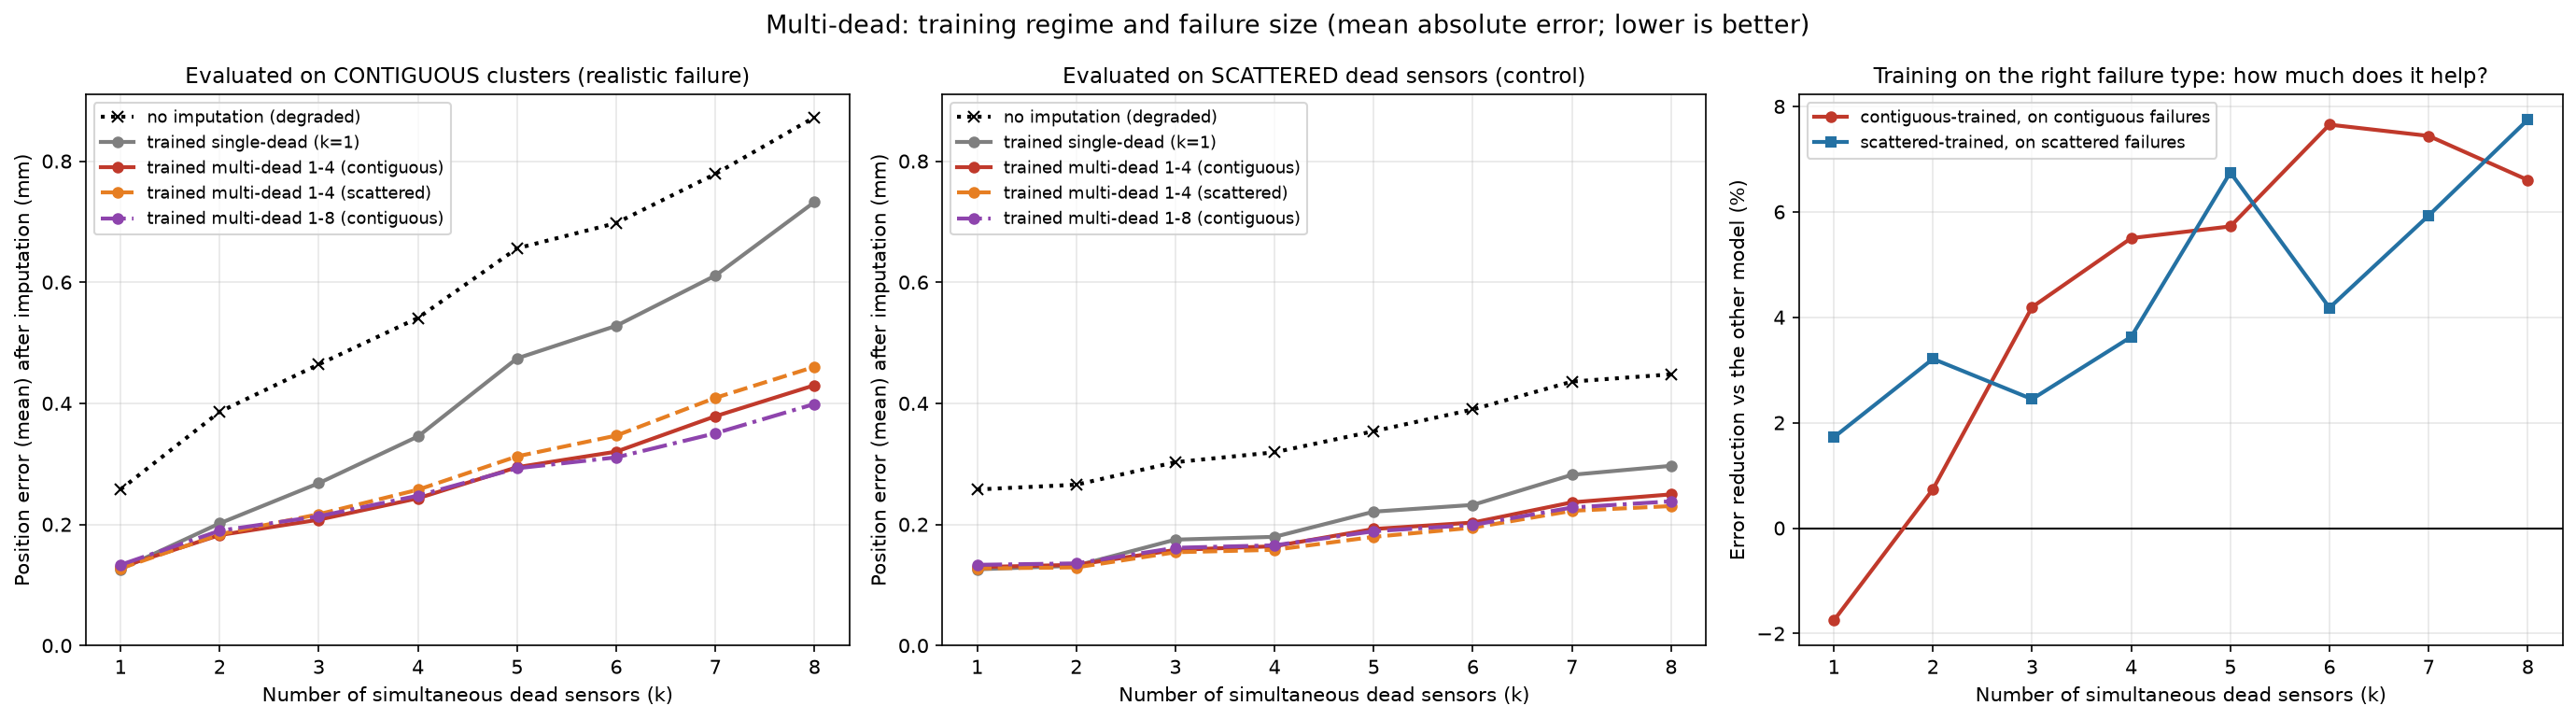
\includegraphics[width=\textwidth]{fig-multidead.png}
\caption{Error absoluto de posición tras la imputación en función del número de sensores averiados
simultáneamente, para los distintos regímenes de entrenamiento. El panel izquierdo corresponde a
fallos contiguos (caso realista) y el central a fallos dispersos (control); el panel derecho
cuantifica la ventaja de entrenar en el régimen que posteriormente se evalúa.}
\label{fig:multidead}
\end{figure}

Como referencia interpretativa, tras la imputación un fallo de ocho sensores contiguos ---el 13\,\%
del detector concentrado en una única región--- deja el módulo en una situación equivalente a la de
un fallo de dos sensores sin imputar, con un error muy inferior al paso entre sensores
(\SI{3.75}{\milli\metre}).

\subsection{Conservación del espectro de energía}
\label{subsec:res-espectro}

La Tabla~\ref{tab:res-espectro} presenta la recuperación espectral estratificada por zonas.

\begin{table}[htbp]
\centering
\caption{Recuperación espectral (\%) por zona del metahexágono y por sensor averiado,
modelo de referencia.}
\label{tab:res-espectro}
\begin{tabular}{lrrr}
\toprule
\textbf{Sensor averiado} & \textbf{Núcleo} & \textbf{Intermedia} & \textbf{Borde} \\
\midrule
$\mathrm{Ich}\,13$ (central) & 96.0 & 85.0 & 52.8 \\
$\mathrm{Ich}\,30$ (intermedio) & 78.6 & 88.7 & 91.7 \\
$\mathrm{Ich}\,32$ (mitad de lado) & 70.0 & 85.5 & 90.5 \\
$\mathrm{Ich}\,27$ (vértice) & 87.2 & 92.0 & 94.4 \\
$\mathrm{Ich}\,31$ (anómalo) & 84.3 & 70.4 & 76.5 \\
\midrule
\textbf{Media} & \textbf{83.2} & \textbf{84.3} & \textbf{81.2} \\
\bottomrule
\end{tabular}
\end{table}

La recuperación espectral se sitúa entre el 77\,\% y el 83\,\% según el sensor averiado, con un
residuo inferior al 0,5\,\% de la posición del fotopico. El resultado es \textbf{uniforme entre
zonas} (83,2 / 84,3 / 81,2), en contraste con la recuperación de posición, donde el borde sufre
apreciablemente más.

Esta disociación admite una interpretación física directa: la conservación de la energía requiere
únicamente acertar la \emph{magnitud} de la carga ausente, mientras que la reconstrucción de la
posición exige además que el \emph{reparto espacial} sea correcto. La estructura por sensor matiza
esta lectura: al enmascarar el sensor central y evaluar los eventos del borde, la recuperación cae
al 52,8\,\%, resultado esperable dado que dichos eventos apenas iluminan el centro del detector.

\subsection{Resolución espacial}
\label{subsec:res-resolucion}

La descomposición del error de posición en sesgo y dispersión arroja los resultados de la
Tabla~\ref{tab:res-resolucion}.

\begin{table}[htbp]
\centering
\caption{Descomposición del error de posición. Agregación macro sobre 61 canales.}
\label{tab:res-resolucion}
\begin{tabular}{lrrr}
\toprule
\textbf{Componente} & \textbf{Degradado} & \textbf{Imputado} & \textbf{Recuperación} \\
\midrule
Sesgo (mm) & 0.126 & 0.022 & 82.7\,\% \\
FWHM / dispersión (mm) & 0.166 & 0.085 & 48.8\,\% \\
\bottomrule
\end{tabular}
\end{table}

El contraste entre ambas componentes es informativo. El \textbf{sesgo se elimina casi por completo}
(82,7\,\%), lo que resulta esperable: el desplazamiento inducido por un canal ausente es sistemático
y por tanto predecible. La \textbf{dispersión se reduce únicamente a la mitad} (48,8\,\%), lo que
refleja el carácter irreducible de la incertidumbre evento a evento: el modelo puede estimar el
valor esperado de la carga ausente, pero no su realización concreta en un evento particular.

El análisis por canal revela que la recuperación mediana de la dispersión es del 51\,\%, con una cola
desfavorable: en dos o tres canales periféricos la mejora es marginal o incluso ligeramente negativa.

\subsection{Ensembles y descomposición sesgo-varianza}
\label{subsec:res-ensemble}

Ambos ensembles superan a la totalidad de sus miembros individuales
(Tabla~\ref{tab:res-ensemble}).

\begin{table}[htbp]
\centering
\caption{Rendimiento de los ensembles frente a la distribución de sus miembros.}
\label{tab:res-ensemble}
\begin{tabular}{lrrrr}
\toprule
\textbf{Configuración} & $\mathcal{R}_{\text{media}}$ & $\mathcal{R}_{p90}$ & \textbf{MAE} & $z$ ($\mathcal{R}_{\text{media}}$) \\
\midrule
Miembros (media $\pm$ desv.) & $52.32 \pm 0.35$ & $58.06 \pm 0.09$ & $0.6220 \pm 0.0026$ & --- \\
Ensemble homogéneo & 52.93 & 58.69 & \textbf{0.6110} & $+1.7$ \\
Ensemble heterogéneo & \textbf{53.21} & \textbf{58.73} & 0.6146 & $+2.5$ \\
\bottomrule
\end{tabular}
\end{table}

El ensemble heterogéneo supera al homogéneo en las métricas de posición, lo que establece que
\textbf{la diversidad arquitectónica aporta más que la diversidad de inicialización}. En el error de
carga, sin embargo, el homogéneo obtiene mejor resultado, lo que se atribuye a que el heterogéneo
incorpora miembros con peor rendimiento en dicha magnitud.

La lectura de mayor calado es la que corresponde a la descomposición sesgo-varianza. Si el error
estuviera dominado por la varianza entre entrenamientos, el promediado de tres modelos lo reduciría
en torno a un 40\,\%; si estuviera dominado por el límite de información, no lo alteraría. La
reducción observada es del \textbf{1,8\,\% en MAE}, de lo que se concluye que aproximadamente el
98\,\% del error es \textbf{irreducible} en el marco planteado.

\subsection{Estimación de incertidumbre}
\label{subsec:res-hetero}

El entrenamiento con la pérdida heterocedástica~\eqref{eq:nll} produjo una degradación severa:
$\mathcal{R}_{\text{media}} = 10.57$, MAE $= 1.31$ y error relativo del 63,2\,\%. La recuperación
mediana resultó \textbf{negativa} ($-18.16$), lo que indica que la imputación deja la posición en
peor situación que la ausencia de imputación.

La causa es un fallo conocido de la formulación: la pérdida~\eqref{eq:nll} permite al modelo reducir
el término cuadrático incrementando $\sigma$, pagando únicamente un coste logarítmico ---y por tanto
lineal en $\log\sigma$--- de modo que le resulta ventajoso sacrificar la precisión de $\mu$ a cambio
de declarar mayor incertidumbre. La corrección estándar consiste en un entrenamiento en dos fases,
con calentamiento bajo error cuadrático puro, o en el empleo de la formulación $\beta$-NLL. Se
documenta como línea de trabajo futuro.

\subsection{Cobertura del conjunto de entrenamiento}
\label{subsec:res-cobertura}

El experimento descrito en la Sección~\ref{subsec:exp-cobertura} arroja un resultado nítido y con
dos caras.

\begin{table}[htbp]
\centering
\caption{Efecto de entrenar con la totalidad de los módulos disponibles, a coste computacional
constante. Agregación macro sobre los 61 canales, \num{600000} eventos por fichero de test en ambos
casos.}
\label{tab:res-cobertura}
\small
\begin{tabular}{lrrr}
\toprule
\textbf{Magnitud} & \textbf{40 módulos} & \textbf{149 módulos} & \textbf{Diferencia} \\
\midrule
$\mathcal{R}_{p90}$ macro (\%) & 58.02 & 57.89 & $-0.13$ \\
$\mathcal{R}_{\text{media}}$ macro (\%) & 52.66 & 52.63 & $-0.02$ \\
$\mathcal{R}_{\text{mediana}}$ macro (\%) & 51.55 & 52.78 & $+1.23$ \\
MAE (ADC) & 0.620 & 0.616 & $-0.004$ \\
\midrule
Desviación entre canales (pts) & 4.49 & \textbf{3.77} & $-16\,\%$ \\
Recorrido entre canales (pts) & 25.2 & \textbf{15.4} & $-39\,\%$ \\
Peor canal (\%) & 38.6 & \textbf{47.9} & $\mathbf{+9.3}$ \\
Canal $\mathrm{Ich}\,31$ (\%) & 38.6 & \textbf{49.5} & $\mathbf{+11.0}$ \\
\bottomrule
\end{tabular}
\end{table}

\paragraph{En el rendimiento medio, ningún efecto.} La comparación pareada canal a canal arroja una
diferencia media de $-0.13$ puntos, con un estadístico $t = -0.49$ que no permite rechazar la
hipótesis nula, y solo 26 de los 61 canales mejoran, proporción indistinguible del azar. La
recuperación media queda en $52.63\,\%$, dentro de la banda de las réplicas
($52.32 \pm 0.35$). \textbf{El límite de rendimiento no procede de la cobertura del entrenamiento},
sino de la información físicamente disponible en los canales supervivientes. Este resultado
convierte en comprobación experimental directa lo que hasta ahora era una inferencia a partir de la
saturación de las distintas variantes arquitectónicas.

\paragraph{En la homogeneidad del detector, un efecto claro.} La dispersión entre canales se reduce
un $16\,\%$ y el recorrido entre el mejor y el peor sensor casi un $40\,\%$. El peor canal pasa de
$38.6\,\%$ a $47.9\,\%$, una mejora de $9.3$ puntos que, contrastada con la banda de las réplicas
para esa misma magnitud ($41.4 \pm 2.52$), corresponde a $z = +2.6$ y resulta por tanto
estadísticamente significativa.

\paragraph{Resolución del comportamiento anómalo de \texorpdfstring{$\mathrm{Ich}\,31$}{Ich 31}.}
Este canal, identificado sucesivamente como sensor defectuoso y como manifestación de la
variabilidad de ganancia entre módulos, mejora $11.0$ puntos al ampliar la cobertura. La
interpretación definitiva es que \textbf{los módulos de test en los que fallaba se encontraban fuera
del régimen estadístico representado en el entrenamiento}: no se trataba de un canal
intrínsecamente problemático, sino de una configuración de detector que el modelo nunca había
observado. Deja de constituir una anomalía del sensor para pasar a ser una manifestación medible de
la cobertura del conjunto de entrenamiento.

\paragraph{Conservación del espectro.} El efecto sobre la métrica energética apunta en la misma
dirección. La recuperación espectral media asciende de $82.9\,\%$ a $86.3\,\%$, y ---de nuevo lo más
relevante--- el peor caso mejora sustancialmente: la combinación más desfavorable, el canal central
evaluado sobre eventos de borde, pasa de $52.8\,\%$ a $65.8\,\%$. Nueve de las quince combinaciones
de canal y zona mejoran.

\paragraph{Resolución espacial y comparación con métodos clásicos.} Las dos magnitudes restantes se
mantienen sin cambios apreciables, lo que resulta coherente con la ausencia de efecto sobre el
rendimiento medio. La recuperación del emborronamiento mejora de forma marginal, de $48.8\,\%$ a
$49.5\,\%$, con una anchura a media altura residual prácticamente idéntica ($0.084$ frente a
$0.085$~mm) y una recuperación del sesgo equivalente ($82.6\,\%$ frente a $82.7\,\%$). La ventaja
sobre la regresión lineal, que sustenta la necesidad del aprendizaje profundo, se conserva en
$11.3$ puntos frente a los $11.5$ del modelo de referencia; la diferencia queda holgadamente dentro
de la variabilidad entre entrenamientos. Ninguno de los dos observables se ve por tanto perjudicado
por la ampliación de la cobertura.

\paragraph{Contrapartida: pérdida de robustez ante fallos múltiples.} La evaluación multi-dead
revela, sin embargo, un efecto de signo contrario que obliga a matizar la valoración. Ambos modelos
se entrenaron exclusivamente con un canal enmascarado, de modo que un fallo de dos o más sensores
constituye para ellos una situación no observada durante el entrenamiento. Con un único canal
averiado, el modelo de cobertura completa es superior, y de forma marcada en el peor caso
($45.9\,\%$ frente a $34.7\,\%$). Pero al aumentar el tamaño del fallo su rendimiento
\textbf{se desploma}: en agrupaciones contiguas de dos sensores la recuperación media cae a valores
negativos ---esto es, la imputación empeora la posición respecto a no imputar--- mientras que el
modelo de referencia se degrada de forma suave y conserva un $49.3\,\%$.

\begin{table}[htbp]
\centering
\caption{Recuperación media (\%) frente al tamaño del fallo, para dos modelos entrenados ambos con
un solo canal enmascarado. Valores negativos indican que la imputación desplaza la posición más de
lo que lo hace el propio fallo.}
\label{tab:res-cobertura-multidead}
\small
\begin{tabular}{lrrrr}
\toprule
\textbf{Modelo} & $k=1$ & $k=2$ & $k=3$ & $k=4$ \\
\midrule
\multicolumn{5}{l}{\emph{Agrupación contigua}} \\
\quad 40 módulos (referencia) & 51.39 & \textbf{49.28} & \textbf{44.21} & \textbf{37.59} \\
\quad 149 módulos & \textbf{51.64} & $-27.35$ & $-123.65$ & $-161.83$ \\
\midrule
\multicolumn{5}{l}{\emph{Fallo disperso}} \\
\quad 40 módulos (referencia) & 51.39 & \textbf{50.71} & \textbf{43.19} & \textbf{43.37} \\
\quad 149 módulos & \textbf{51.64} & 45.13 & 13.62 & $-3.96$ \\
\bottomrule
\end{tabular}
\end{table}

La interpretación más plausible es que el entrenamiento prolongado sobre un régimen de fallo único
---149 épocas frente a 40, con el punto de control seleccionado en la época 133--- produce una
función más ajustada a esa condición concreta y, por ello, más frágil fuera de la distribución de
entrenamiento. La cobertura completa mejora el caso para el que el modelo fue entrenado a costa de
su capacidad de extrapolación.

\paragraph{Implicación práctica.} Ampliar la cobertura no mejora el rendimiento promedio, pero
\textbf{homogeneiza la respuesta del detector sin coste computacional adicional}: eleva el peor
sensor nueve puntos y mejora la conservación del espectro. En un dispositivo real, donde la garantía
relevante es que ningún sensor se degrade de forma catastrófica, ese comportamiento resulta
preferible a una mejora marginal de la media. Ahora bien, la pérdida de robustez ante fallos
múltiples impide recomendar su adopción sin más: un modelo de producción con cobertura completa
debería entrenarse necesariamente en régimen multi-dead
(Sección~\ref{subsec:exp-multidead}), combinando ambas mejoras en lugar de intercambiarlas.

\subsection{Detección de canales defectuosos}
\label{subsec:res-bad}

La Tabla~\ref{tab:res-bad-roc} recoge la validación del estadístico de detección mediante inyección
de fallos con verdad conocida.

\begin{table}[htbp]
\centering
\caption{Validación del detector de canales defectuosos. Área bajo la curva ROC y tasas de
detección en el punto de operación.}
\label{tab:res-bad-roc}
\begin{tabular}{lrrr}
\toprule
\textbf{Severidad del fallo} & \textbf{AUC} & \textbf{TPR} ($Z=2.5$) & \textbf{FPR} \\
\midrule
100\,\% (canal muerto) & 1.000 & 1.000 & 0.009 \\
70\,\% & 0.998 & 0.952 & 0.009 \\
50\,\% & 0.973 & 0.422 & 0.009 \\
30\,\% & 0.868 & 0.091 & 0.009 \\
\bottomrule
\end{tabular}
\end{table}

El estadístico identifica los canales completamente inactivos con separación perfecta
($\mathrm{AUC} = 1.000$) y mantiene un rendimiento elevado para degradaciones severas. La tasa de
falsos positivos en los canales de borde resulta equivalente a la de los canales centrales, lo que
confirma que la normalización por canal resuelve efectivamente el problema del gradiente
estructural.

Las degradaciones moderadas, en cambio, no resultan separables en el punto de operación: si bien el
área bajo la curva indica que la información está presente, explotarla exigiría reducir el umbral y
asumir una tasa de falsos positivos considerablemente mayor.

\begin{figure}[htbp]
\centering
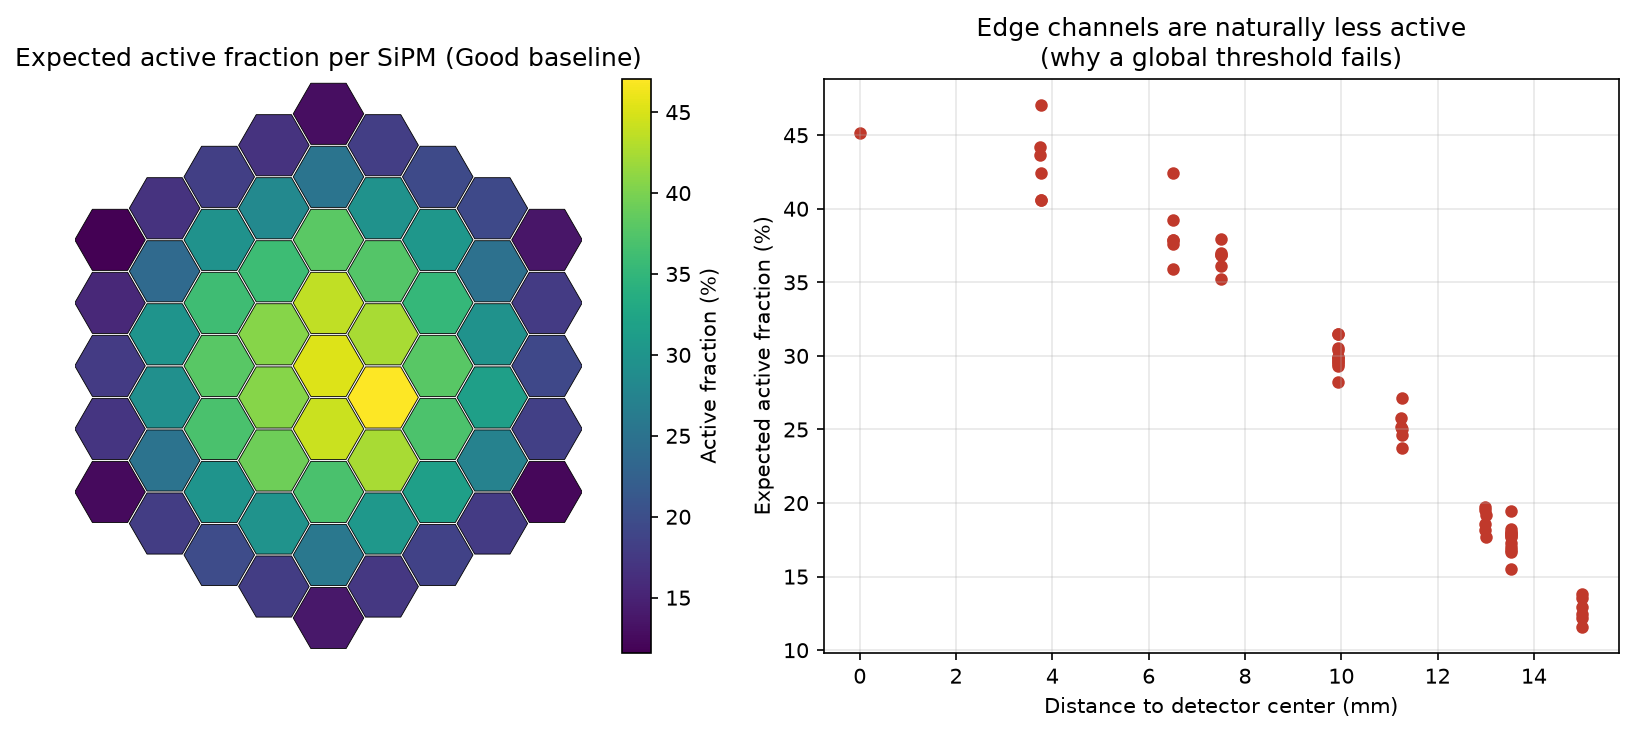
\includegraphics[width=0.95\textwidth]{fig-baseline-bad.png}
\caption{Actividad esperada por sensor en módulos sanos. Izquierda: mapa hexagonal del detector.
Derecha: dependencia con la distancia al centro, con una correlación de $-0.97$. Este gradiente
estructural es la razón por la que un umbral de detección global resulta inadecuado.}
\label{fig:baseline-bad}
\end{figure}

\begin{figure}[htbp]
\centering
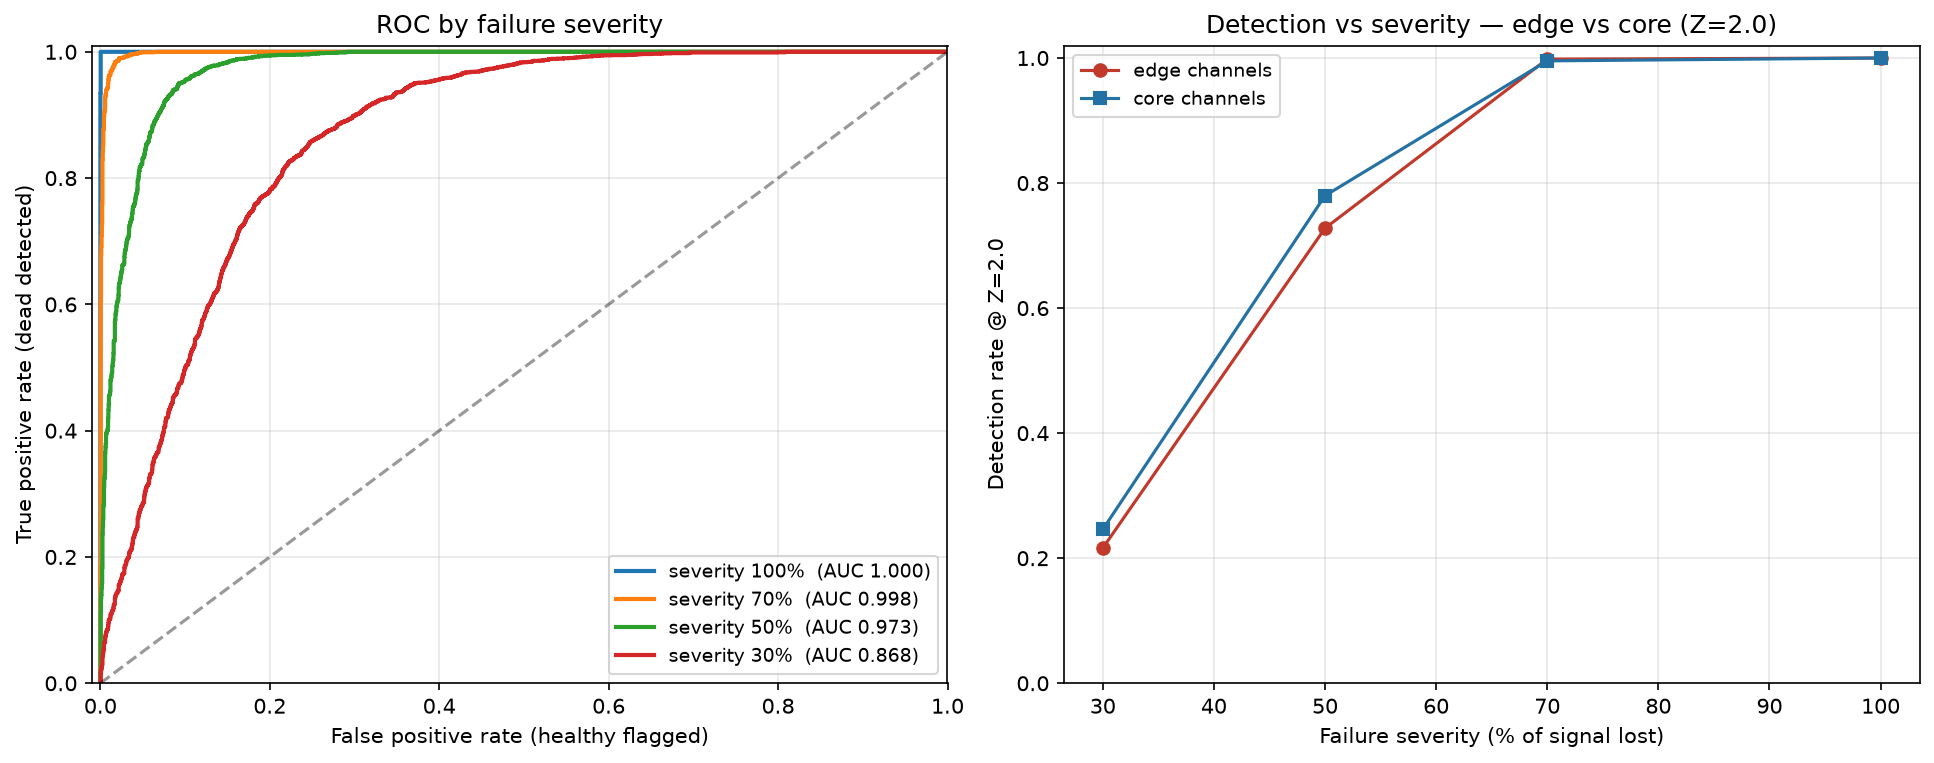
\includegraphics[width=0.95\textwidth]{fig-roc-bad.png}
\caption{Validación del estadístico de detección mediante inyección de fallos con verdad conocida.
Izquierda: curvas ROC para distintas severidades. Derecha: tasa de detección en el punto de
operación, desglosada entre canales de borde y centrales.}
\label{fig:roc-bad}
\end{figure}

Aplicado a los 62 módulos \textsc{Bad} con normalización por módulo y umbral $Z = 2.0$, el
procedimiento identifica canales defectuosos en \textbf{48} de los 62 módulos, marcando
\textbf{278} canales en total, y señala \textbf{12} módulos como globalmente desplazados.



\begin{figure}[htbp]
\centering
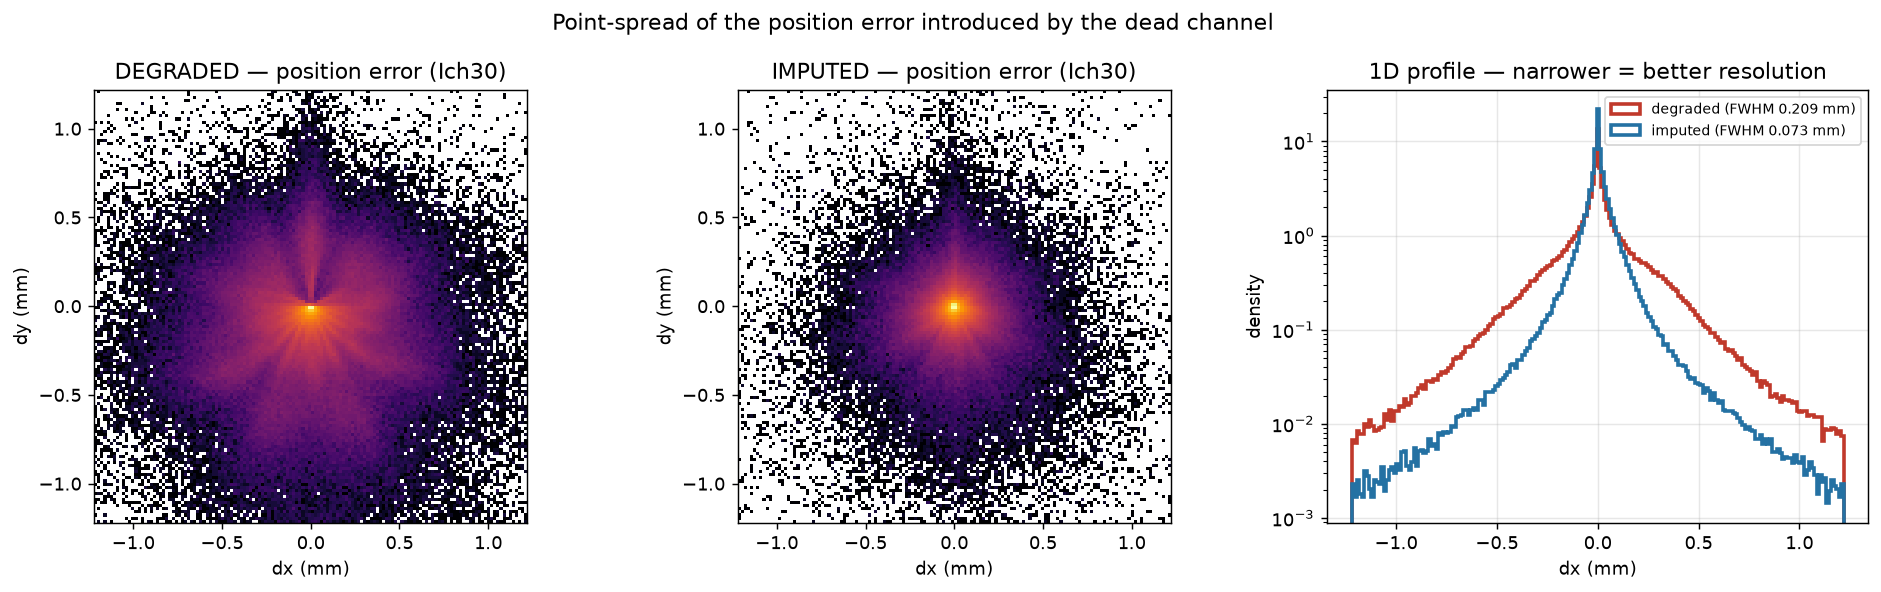
\includegraphics[width=0.95\textwidth]{fig-pointspread.png}
\caption{Distribución bidimensional del error de posición (\emph{point spread}) para el canal
$\mathrm{Ich}\,30$, antes y después de la imputación. La nube de la derecha es simultáneamente más
estrecha (menor dispersión) y está mejor centrada (menor sesgo) que la de la izquierda.}
\label{fig:pointspread}
\end{figure}

\begin{figure}[htbp]
\centering
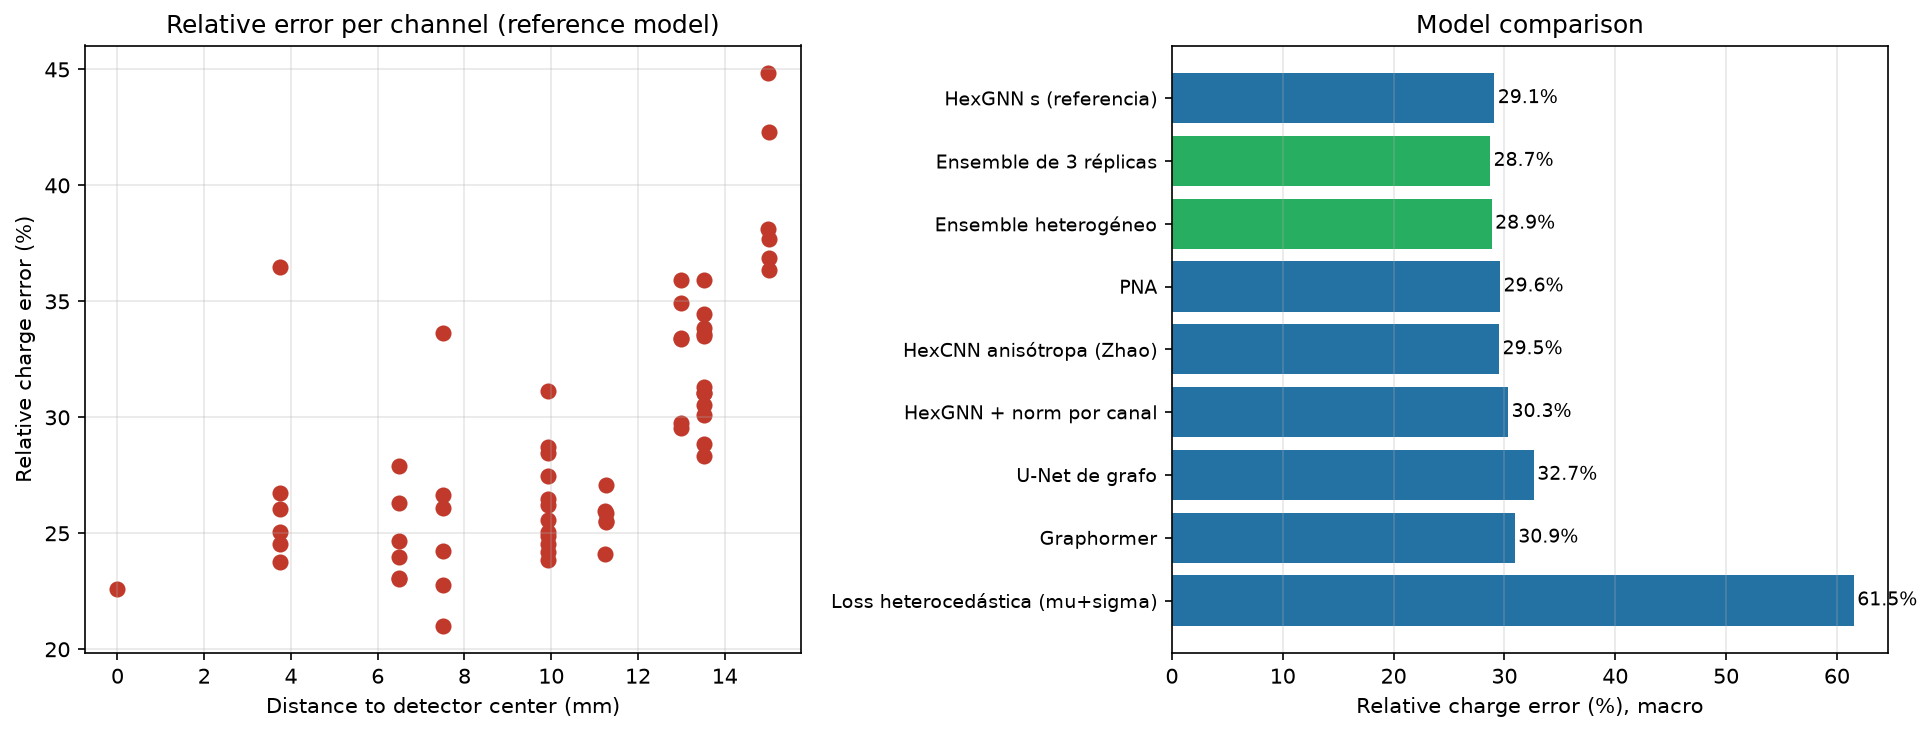
\includegraphics[width=0.95\textwidth]{fig-error-relativo.png}
\caption{Error relativo de carga. Izquierda: valor por canal frente a la distancia al centro del
detector, que evidencia el gradiente centro--borde. Derecha: comparación agregada entre las
configuraciones evaluadas.}
\label{fig:error-relativo}
\end{figure}

\section{Discusión}
\label{sec:discusion}

\subsection{Sobre la naturaleza del límite de rendimiento}

El conjunto de resultados converge de forma consistente hacia una conclusión: el rendimiento
alcanzado no está limitado por la arquitectura ni por la capacidad del modelo, sino por la
\textbf{información físicamente disponible} en los sensores operativos.

Esta conclusión se sustenta en cuatro evidencias independientes. En primer lugar, el incremento de
capacidad no mejora el rendimiento, e incluso lo degrada. En segundo lugar, diez variantes
arquitectónicas ---incluyendo transformadores, arquitecturas multiescala, agregadores múltiples y la
convolución hexagonal canónica--- no superan a la configuración de referencia. En tercer lugar, el
análisis por anillos demuestra que la información explotable se agota en el segundo anillo de
vecindad. Y en cuarto lugar, el ensemble ---que cancela la varianza entre entrenamientos--- recupera
únicamente un 1,8\,\% del error, lo que sitúa en torno al 98\,\% la fracción irreducible.

La descomposición del error de posición en sesgo y dispersión ofrece la interpretación física de
este límite. El sesgo, sistemático y por tanto predecible, se elimina casi por completo. La
dispersión, que corresponde a la incertidumbre sobre la realización concreta de la carga en cada
evento individual, solo se reduce a la mitad. Ninguna arquitectura puede eliminar esta segunda
componente, pues la información necesaria simplemente no está presente en los datos observados.

\subsection{Sobre la adecuación del diseño arquitectónico}

Los resultados permiten justificar el diseño adoptado desde tres perspectivas independientes.

La comparación con métodos clásicos establece que el aprendizaje profundo es \textbf{necesario}: la
red supera en 11,5 puntos a la regresión lineal. El análisis por anillos establece que la
información es \textbf{local}. Y la ablación del grafo establece que el prior geométrico es
\textbf{determinante}. En conjunto, estas tres evidencias caracterizan el modelo adecuado como uno
que sea simultáneamente local, no lineal e informado por la geometría del detector, que es
precisamente la descripción de la arquitectura propuesta.

El análisis de equivarianza añade una cuarta propiedad: la isotropía. La arquitectura respeta por
construcción la simetría $D_6$ del detector, propiedad que las variantes anisótropas rompen sin
obtener contrapartida, dado que el transporte de luz en el cristal es radialmente simétrico.

\subsection{Fortalezas del trabajo}

Cabe destacar como fortalezas metodológicas la definición de un marco de evaluación con significado
físico, que trasciende el error de reconstrucción y cuantifica el impacto sobre posición, energía y
resolución; el diseño diferencial emparejado para la evaluación espectral, que elimina la necesidad
de calibración previa; la estratificación mediante el metahexágono, físicamente motivada por la
geometría del absorbente; la inclusión sistemática de controles ---ablación del grafo, régimen
disperso, control de ruido en $k=1$, réplicas independientes--- que permiten atribuir causalmente los
efectos observados; y la cuantificación explícita de la variabilidad entre entrenamientos, que
proporciona el criterio para juzgar la significación de las comparaciones.

En el plano de los resultados, el hallazgo de que entrenar con fallos múltiples confiere robustez
sin coste alguno en el caso de un único canal tiene aplicabilidad práctica directa.

\subsection{Limitaciones}

\paragraph{Estadística de módulos reducida.} Conviene distinguir esta limitación de la cobertura del
entrenamiento tratada más abajo, con la que resulta fácil confundirla: aquella se refiere a
\emph{cuántos detectores ve el modelo} y afecta a lo que aprende; ésta se refiere a \emph{cuántos
detectores se emplean para medirlo} y afecta a la precisión de la métrica. Son independientes, y el
experimento de cobertura no resuelve la segunda.

La partición reserva únicamente cinco módulos para test. Aunque la estadística de eventos es holgada
---del orden de tres millones---, la de \emph{detectores} es pobre, de modo que las conclusiones
referidas a canales individuales pueden reflejar particularidades de esos cinco módulos concretos.
El caso del canal $\mathrm{Ich}\,31$ ilustra el problema: identificado inicialmente como canal
sistemáticamente anómalo, el análisis posterior reveló que su comportamiento en los módulos de
entrenamiento es normal y que la anomalía se concentra en dos módulos asignados a test; el
experimento de cobertura confirmó después que dichos módulos quedaban fuera del régimen estadístico
representado durante el entrenamiento.

La consecuencia metodológica es que las métricas agregadas carecen de una barra de error asociada al
\emph{efecto de módulo}: se dispone de la variabilidad entre entrenamientos
(Sección~\ref{subsec:res-replicas}), pero no de la variabilidad entre detectores. El procedimiento
descrito en el párrafo anterior ---evaluar sobre los 119 módulos no observados--- permite estimarla
sin reentrenar y se identifica como la comprobación pendiente de mayor valor.

\paragraph{Ausencia de validación cruzada.} No se ha realizado validación cruzada por módulos. La
razón no es el coste ---repetir el entrenamiento cinco veces es perfectamente asumible--- sino que
el número de hiperparámetros a ajustar es reducido y la selección del punto de control ya descansa
en un conjunto de validación independiente. Conviene, no obstante, precisar qué quedaría por
resolver: la validación cruzada no se necesitaría aquí para \emph{ajustar} nada, sino para
\textbf{acotar la sensibilidad de las métricas a qué cinco módulos concretos quedaron reservados
para test}, que es una cuestión distinta y sí pertinente.

Existe, además, una alternativa más económica y estadísticamente más potente que la validación
cruzada para esa pregunta concreta, derivada de la propia mecánica de rotación de ficheros. Puesto
que un modelo de 40 épocas solo llega a ver 40 de los 149 módulos de entrenamiento, los 109
restantes ---junto a los 5 de validación y los 5 de test--- constituyen \textbf{119 módulos que el
modelo no ha observado nunca}. Evaluar sobre ellos proporciona la dispersión entre detectores con
una estadística veinticuatro veces mayor que la del conjunto de test, y sin reentrenar. Es el
procedimiento recomendado para cerrar la limitación descrita en el párrafo siguiente.

\paragraph{Cobertura parcial del conjunto de entrenamiento.} El presupuesto de 40 épocas, combinado
con una rotación cíclica sobre la lista ordenada de ficheros, hace que el modelo utilice 40 de los
149 módulos disponibles, y que sean siempre los mismos. Como se detalla en la
Sección~\ref{subsec:carga-entrenamiento}, ese subconjunto resulta además más homogéneo que la
población completa. El experimento de la Sección~\ref{subsec:res-cobertura} demuestra que esta
limitación \textbf{no afecta al rendimiento medio} ---y por tanto no compromete ninguna de las
comparaciones entre modelos---, pero sí a la \emph{homogeneidad} entre canales: el protocolo de
producción subestima el peor caso en unos nueve puntos. Para trabajo posterior se recomienda adoptar
la cobertura completa, que no conlleva coste adicional.

\paragraph{Ausencia de calibración y filtrado en energía.} El conjunto incluye eventos Compton y de
fondo sin calibración de ganancia. Aunque el diseño diferencial cancela estos efectos en la
evaluación espectral, no puede descartarse que un conjunto calibrado y filtrado permitiera un
rendimiento superior.

\paragraph{Criterio de selección de modelo.} La métrica empleada para seleccionar el punto de
control no rastrea perfectamente el rendimiento en test, como se comprobó en el banco de pruebas.

\paragraph{Alcance del detector de canales defectuosos.} El estadístico desarrollado identifica de
forma fiable los canales inactivos, pero no separa las degradaciones moderadas de la variabilidad
normal, ni detecta canales con ganancia anómalamente elevada, dado que el estadístico es de una sola
cola. La distribución de puntuaciones en los módulos reales no presenta bimodalidad clara, lo que
indica que ``canal defectuoso'' no constituye una categoría con una firma estadística única sino un
conjunto heterogéneo de modos de fallo.

\paragraph{Ausencia de verdad de referencia en los módulos averiados.} La validación del detector se
apoya en fallos inyectados sobre módulos sanos, lo que garantiza una verdad conocida a costa de
evaluar un modo de fallo idealizado. En los módulos defectuosos reales no se dispone de anotación,
de modo que las detecciones no pueden contrastarse y el rendimiento medido no es directamente
extrapolable. La herramienta de etiquetado manual descrita en la Sección~\ref{subsec:exp-bad} se ha
desarrollado precisamente para levantar esta limitación; la anotación de los módulos y la medida del
acuerdo con el estadístico automático constituyen trabajo en curso.

\paragraph{Coste de inferencia del ensemble.} La mejor configuración identificada triplica el coste
de inferencia. Constituye por tanto una mejora en recursos y no en método, extremo que debe
explicitarse al reportar el resultado.

\subsection{Comparación entre aproximaciones}

La comparación entre familias arquitectónicas resulta ilustrativa. Los métodos sin estructura (MLP)
alcanzan recuperaciones del 48--51\,\%. Las arquitecturas basadas en paso de mensajes local se sitúan
en el rango 55--58\,\%. Las basadas en atención global obtienen 54--55\,\%, es decir, peor que las
locales pese a disponer de hasta cien veces más parámetros. La ordenación es coherente con la
naturaleza del problema: la estructura de grafo aporta, mientras que el contexto global no
únicamente no aporta sino que diluye la señal local relevante.

En cuanto a las estrategias de mejora ajenas a la arquitectura, se observa una asimetría notable:
mientras que ninguna modificación arquitectónica superó la referencia, el promediado de modelos sí
produjo una mejora estadísticamente significativa, aunque de magnitud modesta. Esto refuerza la
interpretación de que el margen de mejora disponible no reside en el diseño del modelo.


\section{Conclusiones preliminares}
\label{sec:conclusiones}

\subsection{Respuesta a los objetivos planteados}

\textbf{Sobre el diseño del modelo y el prior geométrico.} Se ha desarrollado una red neuronal de
grafos que explota la adyacencia física de los sensores, alcanzando una recuperación del error de
posición del 52--58\,\% con únicamente \num{38305} parámetros. La ablación del grafo establece de
forma concluyente que dicho prior es el elemento determinante del rendimiento: su eliminación reduce
la recuperación a la mitad.

\textbf{Sobre el marco de evaluación física.} Se ha desarrollado un conjunto de métricas que
cuantifican el impacto de la imputación sobre las tres magnitudes de interés. Los resultados indican
que el método recupera el 52--58\,\% del error de posición, el 77--83\,\% de la conservación del
espectro y el 48,8\,\% de la dispersión espacial, eliminando además el 82,7\,\% del sesgo
sistemático.

\textbf{Sobre la justificación del aprendizaje profundo.} La comparación con métodos clásicos
establece una ventaja de 11,5 puntos frente a la regresión lineal. El análisis por anillos precisa
el origen de dicha ventaja: no procede del acceso a información global ---que resulta irrelevante
más allá del segundo anillo--- sino de la capacidad de modelar relaciones no lineales.

\textbf{Sobre el límite del rendimiento.} El conjunto de evidencias establece que el rendimiento
está limitado por la información disponible y no por el modelo. La formulación de este resultado es
en sí misma una aportación: no se trata de que no se hayan encontrado arquitecturas mejores, sino de
que se ha caracterizado por qué la arquitectura adoptada es la adecuada.

\textbf{Sobre los fallos múltiples.} Entrenar con fallos múltiples contiguos reduce a la mitad el
error con ocho canales averiados, sin penalización alguna en el caso de un único canal, y
generalizando por encima del rango de entrenamiento. El régimen espacial del entrenamiento resulta
relevante, con una ventaja del 6--8\,\% frente a un nivel de ruido del 1,8\,\%.

\textbf{Sobre la detección de canales defectuosos.} Se ha desarrollado un estadístico que identifica
con separación perfecta los canales inactivos, resolviendo el problema del gradiente estructural
centro-borde. Su alcance queda limitado a los fallos severos.

\subsection{Contraste de las hipótesis planteadas}

De las hipótesis formuladas, se confirmaron la relativa al prior geométrico, la relativa a la
localidad de la información, la relativa al mayor daño de los fallos contiguos y la relativa al papel
del ensemble como estimador de la componente reducible del error.

Se refutaron, en cambio, las hipótesis relativas a la utilidad de las pérdidas physics-informed, al
beneficio de incorporar información direccional, a la ventaja de las arquitecturas de mayor
capacidad y a la conveniencia de la normalización por canal. Esta última merece comentario: la
hipótesis predecía una mejora en los canales periféricos, y el resultado fue una degradación
concentrada en los canales centrales. La explicación es que el estimador de posición pondera las
cargas cuadráticamente, de modo que los canales más brillantes dominan la magnitud de interés; la
pérdida cuadrática sin equalizar estaba, de forma no premeditada, alineada con esa ponderación, y
equalizar los canales rompe dicha alineación.

\subsection{Líneas de trabajo futuro}

Se identifican las siguientes líneas de continuación:

\begin{enumerate}
    \item \textbf{Estimación de incertidumbre con formulación corregida}, empleando entrenamiento en
    dos fases o la formulación $\beta$-NLL, con la finalidad de identificar y descartar los eventos
    cuya imputación resulte poco fiable.

    \item \textbf{Ampliación del estadístico de detección} mediante observables sensibles a la forma
    de la distribución de carga y con formulación de dos colas, que permitiría abordar los modos de
    fallo actualmente no cubiertos.

    \item \textbf{Combinación de cobertura completa y entrenamiento multi-canal.} Los resultados de
    la Sección~\ref{subsec:res-cobertura} muestran que ampliar la cobertura de módulos mejora la
    homogeneidad entre sensores y la conservación del espectro, pero degrada la extrapolación a
    fallos múltiples, mientras que el entrenamiento en régimen multi-canal
    (Sección~\ref{subsec:res-multidead}) proporciona precisamente esa robustez sin coste apreciable
    en el caso de fallo único. Al actuar sobre aspectos independientes del procedimiento, ambas
    intervenciones son en principio acumulables, y su combinación constituye la vía más directa
    hacia un modelo de producción que reúna las dos propiedades.

    \item \textbf{Anotación manual completa de los módulos averiados} con la herramienta descrita en
    la Sección~\ref{subsec:exp-bad}, que proporcionaría la verdad de referencia necesaria para medir
    el acuerdo entre el criterio experto y el estadístico automático sobre datos reales, y no
    únicamente sobre fallos inyectados.

    \item \textbf{Validación cruzada por módulos}, que permitiría acotar la sensibilidad de los
    resultados a la partición concreta y robustecer las conclusiones referidas a canales
    individuales.

    \item \textbf{Incorporación de la calibración en energía} y del filtrado correspondiente, con el
    fin de determinar si un conjunto de datos calibrado permite superar el límite observado.

    \item \textbf{Extensión a la corrección de canales anómalos}, generalizando el planteamiento
    desde la imputación de canales ausentes a la corrección de canales con respuesta alterada.

    \item \textbf{Evaluación del impacto sobre la imagen reconstruida}, cerrando la cadena desde la
    recuperación del módulo individual hasta la calidad de la imagen tomográfica final.
\end{enumerate}

% =====================================================================
%  MARCADORES PENDIENTES DE COMPLETAR
% =====================================================================
% TODO(1): Especificar el modelo concreto de SiPM, sus dimensiones activas y el
%          espesor del cristal LYSO. Esta información debe obtenerse de la
%          documentación del sistema experimental o del equipo del laboratorio.
% TODO(2): Detallar la actividad de la fuente de 22Na, la geometría de irradiación
%          y la duración de las adquisiciones.
% TODO(3): Especificar el modelo de ASIC empleado y el valor del umbral de
%          discriminación aplicado.
% TODO(5): Incluir las referencias bibliográficas correspondientes a: GraphSAGE
%          (Hamilton et al., 2017), PNA (Corso et al., 2020), Graphormer (Ying
%          et al., 2021), Graph U-Net (Gao y Ji, 2019), convolución hexagonal
%          (Zhao et al., 2021), beta-NLL (Seitzer et al., 2022), AdamW (Loshchilov
%          y Hutter, 2019) y modified z-score (Iglewicz y Hoaglin, 1993).
% TODO(6): Generar y enlazar las figuras marcadas como [FIGURA SUGERIDA].

\end{document}
.
% =====================================================================

\documentclass[11pt,a4paper]{report}

% ── Codificación e idioma ────────────────────────────────────────────
\usepackage[utf8]{inputenc}
\usepackage[T1]{fontenc}
\usepackage[spanish,es-tabla]{babel}
\usepackage{lmodern}
\usepackage{microtype}

% ── Matemáticas ──────────────────────────────────────────────────────
\usepackage{amsmath}
\usepackage{amssymb}

% ── Tablas y figuras ─────────────────────────────────────────────────
\usepackage{booktabs}
\usepackage{graphicx}
\usepackage{multirow}
\usepackage{siunitx}
\usepackage[font=small,labelfont=bf]{caption}
\usepackage{float}

% ── Formato de página ────────────────────────────────────────────────
\usepackage[a4paper,margin=2.7cm]{geometry}
\usepackage{setspace}
\onehalfspacing
\usepackage{fancyhdr}
\pagestyle{fancy}
\fancyhf{}
\fancyhead[L]{\small\nouppercase{\leftmark}}
\fancyhead[R]{\small\thepage}
\renewcommand{\headrulewidth}{0.4pt}

% ── Enlaces y referencias cruzadas ───────────────────────────────────
\usepackage[colorlinks=true,linkcolor=black,citecolor=black,urlcolor=blue]{hyperref}

% ── Configuración de siunitx (separador decimal español) ─────────────
\sisetup{
  output-decimal-marker = {.},
  group-separator = {\,},
  group-minimum-digits = 4,
  detect-weight = true,
  detect-family = true
}

% ── Ruta de las figuras ──────────────────────────────────────────────
\graphicspath{{figuras/}}

% =====================================================================

\title{%
    \vspace*{2cm}
    {\Huge\bfseries Materiales y métodos}\\[1.2cm]
    {\Large Imputación auto-supervisada de canales SiPM defectuosos\\
     en un detector PET de cristal monolítico hexagonal}\\[0.8cm]
    {\large Trabajo Fin de Máster}
}
\author{Miguel Escudero}
\date{\today}

\begin{document}

\maketitle
\tableofcontents
\listoftables
\listoffigures
\cleardoublepage

\chapter{Materiales y métodos}
\label{cap:materiales-metodos}

\section{Descripción del problema}
\label{sec:descripcion-problema}

\subsection{Contexto: detectores PET de cristal monolítico}
\label{subsec:contexto-pet}

La tomografía por emisión de positrones (PET) reconstruye la distribución espacial de un
radiotrazador emisor de positrones a partir de la detección en coincidencia de los dos fotones
de aniquilación de \SI{511}{\kilo\electronvolt} emitidos en direcciones opuestas. La calidad de
la imagen reconstruida depende de forma crítica de la precisión con que cada módulo detector
determina el punto de interacción del fotón incidente dentro del cristal centelleador.

Históricamente, los detectores PET han empleado matrices de cristales segmentados (\emph{pixelated
arrays}), en los que la posición de interacción se identifica con el cristal individual que
centellea. Esta aproximación desacopla la resolución espacial del proceso de reconstrucción, pero
impone un límite duro: la resolución no puede ser mejor que el tamaño del píxel, y la fracción de
material inactivo entre cristales (el \emph{dead space} de los separadores reflectantes) reduce la
sensibilidad efectiva del sistema.

Los detectores de \textbf{cristal monolítico} constituyen la alternativa que motiva este trabajo.
En ellos, un único bloque continuo de material centelleador ---en el sistema estudiado, un cristal
de ortosilicato de lutecio e itrio dopado con cerio (LYSO)--- se acopla ópticamente a una matriz
de fotomultiplicadores de silicio (SiPM). Cuando un fotón gamma interacciona en el interior del
cristal, la luz de centelleo se propaga isótropamente desde el punto de interacción y genera una
distribución de intensidad continua sobre el plano de sensores. La posición de interacción no se
lee directamente, sino que se \emph{estima} a partir del patrón de reparto de luz entre los
sensores. Esta estrategia elimina el material inactivo entre cristales, mejora la sensibilidad,
y permite en principio una resolución espacial superior al paso entre sensores, además de habilitar
la estimación de la profundidad de interacción (DOI). El precio a pagar es que la reconstrucción
de la posición deja de ser trivial y pasa a depender de un algoritmo de estimación.

El estimador clásico, y el empleado como referencia en este trabajo, es el
\textbf{centro de gravedad ponderado} (\emph{Anger logic}). Dadas las cargas $\{R_c\}_{c=1}^{N}$
registradas por los $N$ sensores situados en posiciones $\{(x_c, y_c)\}$, la posición estimada del
evento se calcula como

\begin{equation}
    \hat{x} = \frac{\sum_{c=1}^{N} R_c^{2}\, x_c}{\sum_{c=1}^{N} R_c^{2}},
    \qquad
    \hat{y} = \frac{\sum_{c=1}^{N} R_c^{2}\, y_c}{\sum_{c=1}^{N} R_c^{2}}.
    \label{eq:centroide}
\end{equation}

El exponente cuadrático sobre las cargas ---en lugar del centro de masas lineal--- concentra el
peso del estimador en los sensores más iluminados, lo que reduce la contribución de las colas de la
distribución de luz y mejora empíricamente la resolución en el interior del cristal. Nótese que la
expresión~\eqref{eq:centroide} es invariante frente a un reescalado global de las cargas
($R_c \rightarrow \alpha R_c$), propiedad que se explotará más adelante al normalizar los eventos.

La representación estándar de la respuesta de un detector monolítico es el \textbf{flood map}: el
histograma bidimensional de las posiciones $(\hat{x}, \hat{y})$ reconstruidas para un gran número de
eventos bajo irradiación uniforme. En un detector sano, el flood map presenta una estructura
característica que refleja tanto la geometría del cristal como la respuesta óptica del conjunto.

\subsection{El problema: canales SiPM defectuosos}
\label{subsec:problema-canales}

La expresión~\eqref{eq:centroide} pone de manifiesto la vulnerabilidad fundamental de los
detectores monolíticos: \textbf{la posición reconstruida depende simultáneamente de todos los
sensores}. Si un canal SiPM deja de funcionar ---y su carga registrada pasa a ser idénticamente
nula--- el numerador y el denominador del estimador se ven alterados de forma sistemática, y la
posición reconstruida se desplaza en dirección opuesta al sensor averiado. El efecto no es un ruido
aleatorio que se promedie a lo largo de la adquisición, sino un \textbf{sesgo estructural} que
distorsiona el flood map completo del módulo.

En un detector segmentado, la avería de un canal implica simplemente la pérdida del cristal
correspondiente: se degrada la sensibilidad, pero la posición de los eventos restantes no se ve
afectada. En un detector monolítico, en cambio, un único canal defectuoso contamina la
reconstrucción de \emph{todos} los eventos cuya distribución de luz alcanzaba a ese sensor. La
consecuencia práctica es que el módulo completo debe descartarse, sustituirse o recalibrarse, con el
coste asociado en tiempo de máquina y en disponibilidad del escáner.

Los modos de fallo observados en el sistema estudiado son heterogéneos. Se han identificado módulos
con un único canal completamente inactivo, módulos con bloques enteros del perímetro apagados
---compatibles con fallos de conexión en serie, sombras mecánicas o efectos térmicos localizados---
y canales que, sin estar muertos, presentan una ganancia anómala. Esta variedad condiciona el diseño
experimental descrito en la Sección~\ref{sec:experimentos}.

\subsection{Planteamiento como problema de imputación auto-supervisada}
\label{subsec:planteamiento}

La propuesta de este trabajo consiste en abordar la avería de un canal como un
\textbf{problema de imputación de datos faltantes}: dado el vector de cargas de los sensores
operativos, estimar la carga que \emph{habría} registrado el sensor averiado, de modo que la
expresión~\eqref{eq:centroide} pueda evaluarse sobre un vector completo y la posición reconstruida
recupere su valor correcto.

Formalmente, sea $\mathbf{R} = (R_1, \dots, R_N) \in \mathbb{R}_{\geq 0}^{N}$ el vector de cargas de
un evento y sea $\mathcal{D} \subset \{1,\dots,N\}$ el conjunto de canales averiados. Se busca una
función $f_\theta$ parametrizada por $\theta$ tal que

\begin{equation}
    \hat{R}_c = f_\theta\!\left(\mathbf{R}_{\setminus \mathcal{D}}, \mathcal{D}\right)_c
    \approx R_c
    \qquad \forall\, c \in \mathcal{D},
    \label{eq:problema-imputacion}
\end{equation}

donde $\mathbf{R}_{\setminus \mathcal{D}}$ denota el vector de cargas con los canales averiados
puestos a cero. La aproximación se juzga no por el error en la carga en sí, sino por su efecto sobre
la magnitud físicamente relevante: la posición reconstruida mediante~\eqref{eq:centroide}.

El aspecto metodológicamente central del planteamiento es su carácter
\textbf{auto-supervisado}. No se dispone de pares (entrada degradada, salida correcta) en los
módulos averiados reales, puesto que la carga verdadera del canal muerto es por definición
inobservable. Sin embargo, sí se dispone de un gran número de módulos \emph{sanos}, en los que es
posible \textbf{simular} la avería: se selecciona un canal, se fuerza su carga a cero, y se emplea
su valor original como etiqueta de supervisión. La supervisión, por tanto, se genera a partir de los
propios datos sin necesidad de anotación externa, lo que sitúa el enfoque en el paradigma del
aprendizaje auto-supervisado por enmascaramiento, análogo conceptualmente a los modelos de lenguaje
enmascarado o a los \emph{masked autoencoders} en visión por computador.

\paragraph{Fundamento físico de la imputabilidad.} Que el problema admita solución no resulta
evidente a priori y conviene justificarlo antes de describir el método. La luz de centelleo
generada por una interacción no se deposita sobre un único fotosensor: el cristal monolítico
reparte el destello sobre una vecindad de SiPM, de modo que la carga de cada canal constituye una
muestra local de una distribución de luz continua y extensa. La información asociada a un sensor
concreto se encuentra, por tanto, \textbf{parcialmente contenida en los sensores que lo rodean}, y
es precisamente esa redundancia la que hace posible reconstruir su valor. El tratamiento
superficial del cristal acota lateralmente la propagación de la luz y confina el destello a una
región de tamaño finito, lo que explica que la redundancia tenga carácter \emph{local}: los vecinos
inmediatos concentran la mayor parte de la información recuperable, mientras que los sensores
alejados apenas aportan. Esta observación anticipa un resultado experimental que se presenta más
adelante (Sección~\ref{subsec:res-anillos}) y motiva el diseño de una arquitectura basada en
vecindades.

Conviene precisar además en qué consiste realmente la tarea que aprende el modelo, pues la
formulación ingenua induce a error. La red no aprende una regla del tipo «si un sensor está apagado,
sustitúyase su valor»: aprende a evaluar si la carga observada en un canal resulta
\textbf{coherente con la distribución de luz que describen los canales restantes}. Para el cálculo
del centroide, por otra parte, no es el valor absoluto de carga de un SiPM lo determinante, sino el
modo en que la luz se reparte entre varios de ellos, lo que refuerza la decisión de normalizar por
evento discutida en la Sección~\ref{subsec:normalizacion}. Esta formulación tiene una consecuencia
práctica inmediata sobre el diseño del muestreo: el modelo debe aprender tanto a corregir cuando la
degradación altera la distribución de luz como a \textbf{abstenerse de corregir} cuando no la
altera, lo que fundamenta físicamente el esquema de balanceo descrito en la
Sección~\ref{subsec:generacion-muestras}.

\subsection{Objetivos}
\label{subsec:objetivos}

El objetivo general del trabajo es \emph{desarrollar y validar un método de imputación de canales
SiPM defectuosos en un detector PET de cristal monolítico que permita recuperar la calidad de
reconstrucción del módulo sin necesidad de sustituir el hardware}. Este objetivo se concreta en los
siguientes objetivos específicos:

\begin{enumerate}
    \item \textbf{Diseñar un modelo de imputación} que explote la estructura geométrica del
    detector, y caracterizar en qué medida dicho prior geométrico contribuye al rendimiento.

    \item \textbf{Establecer el marco de evaluación física} adecuado, que no se limite al error de
    reconstrucción de la carga sino que cuantifique el impacto sobre las magnitudes de interés en
    PET: la posición reconstruida, el espectro de energía y la resolución espacial.

    \item \textbf{Determinar si el aprendizaje profundo está justificado} frente a alternativas
    clásicas de menor complejidad, mediante una comparación rigurosa con métodos de interpolación
    y regresión lineal.

    \item \textbf{Explorar el espacio de arquitecturas} para establecer si el rendimiento obtenido
    está limitado por la capacidad del modelo o por la información físicamente disponible.

    \item \textbf{Extender el método al caso de múltiples canales averiados simultáneamente},
    con especial atención a la configuración físicamente realista de fallos contiguos.

    \item \textbf{Desarrollar un procedimiento de detección} de canales defectuosos que permita
    aplicar el método sobre módulos reales no etiquetados.
\end{enumerate}


\section{Materiales}
\label{sec:materiales}

\subsection{Sistema detector}
\label{subsec:sistema-detector}

El sistema experimental del que proceden los datos consiste en módulos detectores basados en un
cristal centelleador monolítico de LYSO de geometría hexagonal, acoplado a una matriz de SiPM
dispuestos en una retícula hexagonal. La lectura se realiza mediante un circuito integrado de
aplicación específica (ASIC) que digitaliza la carga integrada por cada canal y aplica un umbral de
discriminación para suprimir el ruido electrónico.

La matriz de fotosensores consta de \textbf{64 canales} de lectura, de los cuales \textbf{61 se
encuentran físicamente instrumentados}; los canales con identificadores $\mathrm{Ich} \in
\{1, 16, 18\}$ no disponen de SiPM asociado y se excluyen sistemáticamente del análisis. En lo
sucesivo se emplea una indexación densa $i \in \{0, \dots, 60\}$ sobre los canales activos, junto
con las tablas de conversión correspondientes al identificador físico $\mathrm{Ich}$.

Las posiciones físicas de los 61 sensores se obtienen del fichero de configuración
\texttt{psipm.tsv}. La caracterización geométrica derivada de dichas posiciones se resume en la
Tabla~\ref{tab:geometria-detector}. Cabe destacar que el paso entre sensores vecinos
(\emph{pitch}) es de \SI{3.75}{\milli\metre}, valor que constituye la escala natural de referencia
para interpretar los errores de posición reportados en la Sección~\ref{sec:resultados}.

\begin{table}[htbp]
\centering
\caption{Caracterización geométrica del módulo detector, obtenida de las posiciones físicas
de los sensores.}
\label{tab:geometria-detector}
\begin{tabular}{lc}
\toprule
\textbf{Magnitud} & \textbf{Valor} \\
\midrule
Canales de lectura totales & 64 \\
Canales instrumentados (activos) & 61 \\
Canales inactivos ($\mathrm{Ich}$) & 1, 16, 18 \\
Paso entre sensores vecinos (\emph{pitch}) & \SI{3.75}{\milli\metre} \\
Extensión en $x$ & $[-13.0,\ 13.0]$~mm \\
Extensión en $y$ & $[-15.0,\ 15.0]$~mm \\
Radio máximo desde el centro & \SI{15.01}{\milli\metre} \\
Geometría de la retícula & Hexagonal (hexágono de lado 5) \\
\bottomrule
\end{tabular}
\end{table}

Un aspecto físico determinante para la interpretación de los resultados es la presencia de un
\textbf{adhesivo absorbente (negro) en las caras laterales del cristal}. Su función es suprimir las
reflexiones en los bordes, que de otro modo degradarían la estimación de posición, pero tiene como
efecto colateral que los eventos que interaccionan cerca del perímetro pierden una fracción
significativa de la luz de centelleo. Este hecho, confirmado por el análisis de los datos, se
traduce en dos observaciones recurrentes a lo largo del trabajo: los sensores del borde registran
sistemáticamente menos carga que los centrales, y el fotopico de energía se desplaza hacia energías
menores en las regiones periféricas del cristal.

\begin{figure}[htbp]
\centering
% \includegraphics[width=0.6\textwidth]{figuras/geometria_detector.pdf}
\caption{\textbf{[FIGURA SUGERIDA]} Disposición de los 61 SiPM activos sobre el plano del detector,
con la retícula hexagonal y la numeración $\mathrm{Ich}$ de cada canal. Se recomienda superponer el
contorno del cristal y señalar la posición del adhesivo absorbente en las caras laterales.}
\label{fig:geometria-detector}
\end{figure}

\subsection{Entorno software}
\label{subsec:entorno-software}

La totalidad del desarrollo se ha realizado en Python sobre un entorno gestionado con
\texttt{conda}. La Tabla~\ref{tab:entorno-software} recoge las versiones exactas de los componentes
empleados, información necesaria para garantizar la reproducibilidad de los experimentos.

\begin{table}[htbp]
\centering
\caption{Entorno software y hardware empleado en el desarrollo y la experimentación.}
\label{tab:entorno-software}
\begin{tabular}{lll}
\toprule
\textbf{Componente} & \textbf{Versión} & \textbf{Función en el trabajo} \\
\midrule
Python & 3.11.15 & Lenguaje de implementación \\
PyTorch & 2.5.1+cu121 & Definición y entrenamiento de los modelos \\
CUDA & 12.1 & Aceleración por GPU \\
NumPy & 2.4.4 & Álgebra y manipulación de arrays \\
SciPy & 1.17.1 & \texttt{cKDTree}, \texttt{ConvexHull}, distancia de Wasserstein \\
Matplotlib & 3.11.0 & Generación de figuras \\
openpyxl & 3.1.5 & Exportación de tablas de métricas \\
Weights \& Biases & 0.28.0 & Registro y trazabilidad de experimentos \\
\midrule
GPU & NVIDIA GTX 1660 SUPER & Entrenamiento e inferencia \\
Sistema operativo & Windows 11 & Entorno de ejecución \\
\bottomrule
\end{tabular}
\end{table}

La elección de PyTorch como \emph{framework} responde a la necesidad de implementar operadores de
paso de mensajes sobre un grafo con topología fija y no estándar. Aunque existen bibliotecas
especializadas en redes de grafos (\texttt{PyTorch Geometric}, \texttt{DGL}), se optó
deliberadamente por una implementación directa con tensores densos. Esta decisión se justifica por
tres motivos: el grafo del detector es pequeño ($N = 61$ nodos) y \emph{fijo}, lo que hace que la
indexación densa sea más eficiente que las estructuras dispersas generales; se elimina una
dependencia externa cuyo ciclo de versiones es sensible a la de PyTorch; y, sobre todo, se mantiene
control explícito sobre la operación de agregación, aspecto que resulta central en los experimentos
de la Sección~\ref{sec:experimentos}.

\subsection{Herramientas de desarrollo y trazabilidad}
\label{subsec:herramientas}

El control de versiones del código se ha realizado con Git, sobre un repositorio alojado en GitHub.
El seguimiento de los experimentos de entrenamiento y evaluación se ha llevado a cabo con
Weights~\&~Biases, registrando de forma sistemática los hiperparámetros, las curvas de entrenamiento
y las figuras resultantes de cada evaluación. Los procesos de entrenamiento y evaluación se
registran como ejecuciones diferenciadas mediante el campo \texttt{job\_type}, lo que permite
trazar qué evaluación corresponde a qué modelo.

Adicionalmente, se ha mantenido un cuaderno de laboratorio en formato Markdown en el que se han
documentado de forma cronológica las decisiones metodológicas, los resultados obtenidos y ---de
manera explícita--- las hipótesis descartadas y los errores de interpretación detectados y
corregidos. Esta práctica ha resultado determinante para la coherencia del trabajo, dado el elevado
número de experimentos realizados.

\subsection{Organización del código}
\label{subsec:organizacion-codigo}

La implementación se estructura en módulos con responsabilidades bien delimitadas, cuya
descripción funcional se recoge en la Tabla~\ref{tab:modulos-codigo}. El diseño responde al
principio de \emph{fuente única de verdad}: elementos críticos como la partición de los datos o la
construcción del grafo de vecindad se definen en un único lugar y son importados por el resto de
módulos, de modo que resulta imposible que el entrenamiento y la evaluación operen sobre
configuraciones discrepantes.

\begin{table}[htbp]
\centering
\caption{Módulos principales de la implementación y su responsabilidad.}
\label{tab:modulos-codigo}
\small
\begin{tabular}{p{0.26\textwidth}p{0.66\textwidth}}
\toprule
\textbf{Módulo} & \textbf{Responsabilidad} \\
\midrule
\texttt{dataset.py} & Lectura del formato binario, densificación, generación de muestras
    auto-supervisadas \emph{on-the-fly} y partición reproducible de los ficheros. \\
\texttt{hex\_geometry.py} & Construcción del grafo de vecindad, vectores de arista, matriz de
    vecindad direccional y escala característica por canal. \\
\texttt{model.py} & Definición de las arquitecturas de producción y del ensemble. \\
\texttt{train.py} & Bucle de entrenamiento, funciones de pérdida y selección de modelo. \\
\texttt{imputation\_eval.py} & Carga de modelos, rutina de imputación y evaluación monocanal. \\
\texttt{eval\_total.py} & Evaluación multicanal sobre los 61 sensores y análisis por líneas. \\
\texttt{eval\_espectro.py} & Conservación del espectro de energía estratificada por zonas. \\
\texttt{eval\_multidead.py} & Barrido de tamaño de fallo y régimen espacial. \\
\texttt{eval\_resolution.py} & Descomposición del error de posición en sesgo y dispersión. \\
\texttt{eval\_baselines.py} & Comparación con métodos clásicos. \\
\texttt{eval\_linear\_rings.py} & Análisis de localidad de la información mediante regresión por anillos. \\
\texttt{sandbox\_arch*.py} & Banco de pruebas de arquitecturas alternativas. \\
\texttt{bad\_detect.py} & Estadístico de detección de canales defectuosos. \\
\texttt{bad\_validate.py} & Validación del detector con verdad conocida por inyección. \\
\texttt{bad\_label.py} & Interfaz de etiquetado manual asistido de los módulos averiados. \\
\bottomrule
\end{tabular}
\end{table}


\section{Conjunto de datos}
\label{sec:datos}

\subsection{Origen y naturaleza de los datos}
\label{subsec:origen-datos}

Los datos proceden de adquisiciones experimentales realizadas sobre módulos detectores irradiados
con una fuente de $^{22}$Na. Este isótopo es un emisor de positrones cuyo espectro de energía
presenta dos líneas características: el fotopico de aniquilación a \SI{511}{\kilo\electronvolt} y
una segunda línea a \SI{1275}{\kilo\electronvolt} procedente de la desexcitación del núcleo hijo.
La presencia de estas líneas en el espectro de energía reconstruido se ha empleado como control de
calidad de los datos.

Es importante señalar que las adquisiciones se registran en modo \emph{singles}, es decir, cada
evento se almacena sin aplicar filtro de coincidencia. Esto implica que el conjunto contiene tanto
eventos de fotopico como eventos de dispersión Compton y sucesos de fondo, lo que amplía el rango
dinámico de las cargas registradas y constituye un factor a considerar en la interpretación de los
espectros.

El conjunto de datos se organiza en dos poblaciones diferenciadas:

\begin{itemize}
    \item \textbf{Módulos \textsc{Good}}: \textbf{159 ficheros}, correspondientes a módulos cuyos
    61 canales se consideran operativos. Constituyen la base para el entrenamiento y para toda la
    evaluación con verdad de referencia conocida.

    \item \textbf{Módulos \textsc{Bad}}: \textbf{62 ficheros}, correspondientes a módulos con uno o
    más canales defectuosos. No disponen de etiquetado: se desconoce a priori qué canales fallan y
    en qué grado. Se emplean exclusivamente en la fase de aplicación y validación cualitativa
    (Sección~\ref{subsec:exp-bad}).
\end{itemize}

Cada fichero corresponde a un módulo físico distinto del escáner, con un volumen medio de
\SI{161}{\mega\byte} y del orden de $10^6$ eventos. El volumen total del conjunto \textsc{Good}
asciende aproximadamente a \SI{25.5}{\giga\byte}, magnitud que ha condicionado de forma directa la
estrategia de carga de datos descrita en la Sección~\ref{subsec:generacion-muestras}.

\subsection{Formato binario y lectura}
\label{subsec:formato-binario}

Los ficheros \texttt{.dat} emplean un formato binario compacto de longitud variable por evento,
diseñado para almacenar únicamente los canales que superan el umbral del ASIC. La estructura de
cada evento es la siguiente:

\begin{enumerate}
    \item Un byte sin signo, $N_{\text{int}}$, que indica el número de canales que han registrado
    señal en el evento.
    \item A continuación, $N_{\text{int}}$ registros consecutivos de 8 bytes, cada uno compuesto por
    un valor de carga en coma flotante de precisión simple (\texttt{float32}, \emph{little-endian})
    seguido del identificador de canal como entero de 32 bits (\texttt{int32}).
\end{enumerate}

La lectura se implementa cargando el fichero completo en memoria y recorriéndolo mediante una vista
sin copia (\texttt{memoryview}), interpretando cada bloque de registros con
\texttt{numpy.frombuffer} sobre un \texttt{dtype} estructurado. Esta estrategia evita el
procesamiento byte a byte en Python, que resultaría prohibitivo para conjuntos de millones de
eventos.

El resultado de la lectura es la \textbf{densificación} del evento: el formato disperso
$(R_c, \mathrm{Ich}_c)$ se convierte en un vector denso de dimensión 61, en el que los canales que no
superaron el umbral toman valor cero. Esta representación densa y de dimensión fija es la que
consume el modelo.

Conviene subrayar que la \emph{sparsity} observada ---en promedio, únicamente \textbf{17 de los 61
canales} registran señal en un evento dado--- no constituye un defecto de los datos ni una pérdida
de información recuperable, sino el comportamiento nominal del sistema: el ASIC aplica un umbral de
discriminación para suprimir el ruido electrónico térmico, de modo que un canal a cero indica que el
sistema de adquisición ya determinó que no había señal significativa. Esta interpretación es
relevante porque justifica la definición de la etiqueta interna descrita en la
Sección~\ref{subsec:generacion-muestras}.

\subsection{Caracterización estadística}
\label{subsec:caracterizacion-datos}

La Tabla~\ref{tab:caracterizacion-datos} resume las propiedades estadísticas del conjunto,
obtenidas sobre los ficheros de la partición de test.

\begin{table}[htbp]
\centering
\caption{Caracterización estadística del conjunto de datos.}
\label{tab:caracterizacion-datos}
\begin{tabular}{lc}
\toprule
\textbf{Magnitud} & \textbf{Valor} \\
\midrule
Ficheros \textsc{Good} & 159 \\
Ficheros \textsc{Bad} & 62 \\
Tamaño medio por fichero & \SI{161}{\mega\byte} \\
Volumen total (\textsc{Good}) & \SI{25.5}{\giga\byte} \\
Eventos por fichero (orden de magnitud) & $\sim 10^6$ \\
Eventos totales en la partición de test & \num{5476642} \\
Canales activos por evento (media) & 17.0 \\
Canales activos por evento (rango) & 1--54 \\
Carga total por evento, $R_T$ (media) & 31.9 (ADC) \\
Carga total por evento, $R_T$ (mediana) & 26.8 (ADC) \\
\bottomrule
\end{tabular}
\end{table}

La diferencia entre la media y la mediana de la carga total por evento ($31.9$ frente a $26.8$)
evidencia la asimetría de la distribución de energía, consistente con la presencia de una cola de
eventos de alta energía sobre un fondo Compton dominante.

\subsection{Limpieza y preprocesado}
\label{subsec:preprocesado}

El preprocesado aplicado ha sido deliberadamente mínimo, con el fin de evitar la introducción de
sesgos no controlados. Las operaciones realizadas, y su justificación, son las siguientes.

\paragraph{Tratamiento de cargas negativas.} Una fracción de los valores de carga registrados es
negativa. Estos valores no corresponden a señal física, sino a artefactos de la cadena de lectura:
parámetros de calibración que no ajustan correctamente el rango dinámico del ADC, o errores de
conexión. Se aplica un recorte a cero,
\begin{equation}
    R_c \leftarrow \max(R_c, 0),
\end{equation}
en lugar del valor absoluto. Esta elección, validada con el equipo experimental, es la
metodológicamente correcta: tomar el valor absoluto \emph{inventaría} señal donde no la hay,
mientras que el recorte se limita a reconocer la ausencia de señal significativa.

\paragraph{Descarte de eventos vacíos.} Se eliminan los eventos cuya carga total resulta nula tras
el recorte. Estos sucesos no aportan información y, además, provocarían una división por cero en la
normalización descrita más adelante.

\paragraph{Ausencia de filtrado en energía.} Se ha decidido \textbf{no} aplicar ningún filtro de
selección en energía (por ejemplo, una ventana en torno al fotopico de \SI{511}{\kilo\electronvolt}).
La justificación es doble. En primer lugar, un filtrado riguroso requeriría una calibración en
energía previa ---la alineación de los fotopicos canal a canal--- que no está disponible y cuya
obtención excede el alcance del trabajo. En segundo lugar, el filtrado reduciría sustancialmente el
tamaño del conjunto de entrenamiento sin una ventaja clara: el objetivo del modelo es reconstruir la
carga de un canal a partir de los restantes, tarea que no depende de que el evento pertenezca al
fotopico. Se documenta, no obstante, como limitación en la Sección~\ref{sec:discusion}.

\paragraph{Ausencia de calibración en energía.} Por el mismo motivo, no se ha aplicado corrección de
ganancia canal a canal. Esta decisión tiene una implicación metodológica importante que se ha
explotado deliberadamente en el diseño de la evaluación del espectro
(Sección~\ref{subsec:met-espectro}): al emplear un diseño \emph{diferencial emparejado} sobre los
mismos eventos, los efectos de la falta de calibración se cancelan y no contaminan la métrica.

\subsection{Normalización por evento}
\label{subsec:normalizacion}

Cada muestra se normaliza dividiendo el vector de cargas por un factor de escala calculado
\textbf{a nivel de evento} y, de forma crítica, \textbf{después} de aplicar el enmascaramiento:

\begin{equation}
    \eta = \max_{c \notin \mathcal{D}} R_c,
    \qquad
    \mathbf{x}^{\text{in}} = \frac{\mathbf{R}_{\setminus \mathcal{D}}}{\eta},
    \qquad
    \mathbf{y}^{\text{target}} = \frac{\mathbf{R}}{\eta}.
    \label{eq:normalizacion}
\end{equation}

La normalización por evento fue recomendada por el equipo experimental con el fin de evitar
oscilaciones en el entrenamiento derivadas de las variaciones de calibración entre módulos. Su
fundamento físico es que la información relevante para localizar el punto de interacción reside en
la \emph{distribución relativa} de la luz entre sensores, no en su magnitud absoluta; obsérvese que
el estimador~\eqref{eq:centroide} es efectivamente invariante a esta escala.

Dos consecuencias del esquema~\eqref{eq:normalizacion} merecen comentario explícito:

\begin{itemize}
    \item \textbf{Entrada y objetivo comparten el mismo factor $\eta$.} Esto es necesario para que
    la predicción sea reescalable a unidades físicas, pero implica que si el canal enmascarado era el
    más brillante del evento, entonces $y^{\text{target}}_c > 1$. Por este motivo la salida de todas
    las redes es \textbf{estrictamente lineal}, sin función de activación acotante (sigmoide o
    recorte) en la última capa: acotar la salida haría imposible predecir correctamente esos casos.

    \item \textbf{El factor depende de un único canal.} Al emplear el máximo, la escala del evento
    queda determinada por el sensor más iluminado. Esta dependencia se identificó como una posible
    fuente de fragilidad y motivó el experimento descrito en la Sección~\ref{subsec:exp-norm}, en el
    que se evaluó una normalización alternativa basada en la suma.
\end{itemize}

\subsection{Generación de muestras auto-supervisadas}
\label{subsec:generacion-muestras}

La generación de las muestras de entrenamiento se realiza \textbf{al vuelo} (\emph{on-the-fly}),
sin materializar en disco el conjunto de pares (entrada, objetivo). La razón es dimensional: con
$\sim 10^6$ eventos por fichero, 159 ficheros y 61 posibles canales a enmascarar por evento, el
conjunto completo de muestras posibles sería del orden de $10^{10}$, inviable de almacenar. La
generación dinámica permite además que el enmascaramiento cambie en cada época, lo que actúa como
una forma natural de aumento de datos.

El procedimiento para cada muestra es el siguiente:

\begin{enumerate}
    \item Se toma un evento sano $\mathbf{R}$ del fichero cargado en la época actual.
    \item Se selecciona el canal (o conjunto de canales) a enmascarar según la política de balanceo
    descrita a continuación.
    \item Se anula la carga de dichos canales y se normaliza según~\eqref{eq:normalizacion}.
    \item Se construye la entrada como una matriz de dos filas y 61 columnas: la primera contiene
    las cargas normalizadas con los canales enmascarados a cero, y la segunda una máscara binaria
    que indica explícitamente qué canales han sido enmascarados.
    \item El objetivo es el vector original completo, normalizado con el mismo factor.
\end{enumerate}

La inclusión explícita de la máscara como segunda fila de la entrada es una decisión de diseño
relevante: sin ella, el modelo no podría distinguir entre un canal enmascarado y un canal que
legítimamente no superó el umbral, dado que ambos aparecen como ceros.

\paragraph{Balanceo \emph{modified} / \emph{non-modified}.} Se define una etiqueta interna ---no
visible para el modelo--- que clasifica cada muestra según si el canal enmascarado tenía o no señal:

\begin{itemize}
    \item Muestra \textbf{\emph{modified}}: el canal enmascarado tenía carga no nula. El vector de
    entrada difiere realmente del original y el modelo debe imputar un valor.
    \item Muestra \textbf{\emph{non-modified}}: el canal enmascarado ya valía cero. El modelo debe
    aprender a \emph{no} corregir cuando no procede.
\end{itemize}

El muestreo fuerza una proporción \textbf{50/50} entre ambas clases mediante la paridad del índice
de la muestra, de modo que con un \texttt{DataLoader} configurado con \texttt{shuffle=True} cada
lote contiene aproximadamente la misma cantidad de ambas. La justificación es que, dada la
\emph{sparsity} del sistema (17 de 61 canales activos en promedio), un muestreo uniforme produciría
en torno a un 72\,\% de muestras \emph{non-modified}, sesgando el modelo hacia la inacción. Se optó
por conservar las muestras \emph{non-modified} en lugar de descartarlas porque enseñan una capacidad
necesaria: reconocer cuándo la respuesta correcta es cero.

La definición operativa de ``cero'' es la que resulta del recorte, sin introducir umbrales
adicionales. Como se argumentó en la Sección~\ref{subsec:formato-binario}, el umbral ya lo aplicó el
hardware; un canal a cero es un canal que el sistema de adquisición consideró sin señal.

\subsection{Partición de los datos}
\label{subsec:particion}

La partición del conjunto \textsc{Good} se realiza \textbf{a nivel de fichero}, no de evento, en la
proporción \textbf{149 / 5 / 5} (entrenamiento / validación / test). El barajado previo emplea una
semilla fija ($\texttt{seed} = 42$), lo que garantiza la reproducibilidad exacta de la partición.
La composición resultante se detalla en la Tabla~\ref{tab:particion}.

\begin{table}[htbp]
\centering
\caption{Partición del conjunto \textsc{Good} (semilla 42). Cada fichero corresponde a un módulo
detector físico distinto.}
\label{tab:particion}
\begin{tabular}{lcl}
\toprule
\textbf{Partición} & \textbf{N.º ficheros} & \textbf{Identificadores} \\
\midrule
Entrenamiento & 149 & (los restantes) \\
Validación & 5 & datas013, datas015, datas080, datas142, datas182 \\
Test & 5 & datas057, datas116, datas126, datas202, datas214 \\
\bottomrule
\end{tabular}
\end{table}

La decisión de particionar por fichero, y no por evento, es metodológicamente central. Dado que cada
fichero corresponde a un módulo físico distinto, con sus propias particularidades de calibración y
ganancia, esta partición mide la capacidad de \textbf{generalización a detectores no vistos}, que es
la condición de uso real del método. Una partición por evento habría permitido que eventos del mismo
módulo aparecieran simultáneamente en entrenamiento y test, produciendo una estimación
optimista del rendimiento por memorización de las idiosincrasias de cada módulo.

La partición se define en una única función (\texttt{dataset.get\_file\_split}) importada tanto por
el bucle de entrenamiento como por todos los evaluadores, lo que hace estructuralmente imposible que
un fichero de test se emplee inadvertidamente durante el entrenamiento.

\paragraph{Limitación reconocida.} La partición proporciona una estadística de \emph{eventos}
holgada (más de 5.4 millones en test) pero una estadística de \emph{módulos} reducida (5 módulos).
En consecuencia, las métricas agregadas son robustas, mientras que las conclusiones referidas a
canales individuales pueden reflejar idiosincrasias de los módulos concretos que integran la
partición de test. Esta limitación se manifestó de forma concreta en el análisis del canal
$\mathrm{Ich}\,31$ y se discute en la Sección~\ref{sec:discusion}.

\subsection{Estrategia de carga durante el entrenamiento}
\label{subsec:carga-entrenamiento}

Dado que el conjunto completo no cabe en memoria, se emplea una \textbf{rotación de ficheros}: en
cada época se carga un único fichero de entrenamiento, seleccionado cíclicamente, del que se toman
hasta \num{400000} eventos. Con un presupuesto de 40 épocas, el modelo ve por tanto 40 módulos
distintos, cada uno una sola vez.

Esta estrategia tiene una consecuencia favorable: al no repetirse nunca exactamente la misma muestra
(el enmascaramiento se re-sortea con una semilla dependiente de la época), el modelo opera en un
régimen efectivo de datos prácticamente infinitos, lo que reduce drásticamente el riesgo de
sobreajuste y justifica la decisión de entrenar el presupuesto completo de épocas sin parada
temprana.

El conjunto de validación, por el contrario, se carga \textbf{una única vez} y con una semilla de
enmascaramiento \textbf{fija}, de modo que la métrica de validación es exactamente comparable entre
épocas y entre modelos.

\paragraph{Cobertura efectiva del conjunto de entrenamiento.} La rotación cíclica sobre una lista
ordenada implica que los 40 módulos empleados no son una muestra aleatoria de los 149 disponibles,
sino los 40 primeros en orden de numeración. Una inspección posterior de las estadísticas por módulo
revela que ese subconjunto es \textbf{sensiblemente más homogéneo} que el conjunto completo: la
desviación típica del número medio de canales activos por evento es de $0.37$ entre los módulos
vistos, frente a $2.28$ entre los no vistos. El modelo se entrena, por tanto, en un régimen más
estrecho que el que representa la población real de detectores, y alguno de los módulos reservados
para test queda apreciablemente fuera de ese régimen. Esta observación resulta relevante al
interpretar tanto el comportamiento del canal $\mathrm{Ich}\,31$ como el techo de rendimiento
descrito en los resultados, y motivó el experimento controlado que se presenta en la
Sección~\ref{subsec:exp-cobertura}, cuyo desenlace permite descartar la cobertura como causa del
límite observado.


\section{Arquitecturas y modelos}
\label{sec:arquitecturas}

Esta sección describe las arquitecturas implementadas. Se presentan en orden de complejidad
estructural creciente, comenzando por los baselines sin estructura y culminando en el modelo de
referencia adoptado. Todas comparten la misma interfaz: reciben un tensor de entrada de dimensión
$(B, 2, 61)$ y producen una salida de dimensión $(B, 61)$ con las cargas reconstruidas.

\subsection{Baselines clásicos sin aprendizaje profundo}
\label{subsec:baselines-clasicos}

Antes de justificar el uso de redes neuronales resulta imprescindible establecer el rendimiento de
métodos elementales. Se han implementado dos:

\paragraph{Interpolación por media de vecinos.} La estimación más simple posible: la carga del canal
averiado se aproxima por la media aritmética de las cargas de sus vecinos físicos inmediatos,
\begin{equation}
    \hat{R}_c = \frac{1}{|\mathcal{N}(c)|} \sum_{j \in \mathcal{N}(c)} R_j,
\end{equation}
donde $\mathcal{N}(c)$ denota el conjunto de vecinos del sensor $c$ en el grafo del detector. Este
método no requiere entrenamiento alguno.

\paragraph{Regresión lineal por canal.} Para cada canal $c$ se ajusta por mínimos cuadrados un
modelo lineal que predice su carga a partir de los 60 canales restantes,
\begin{equation}
    \hat{R}_c = \mathbf{w}_c^{\top} \mathbf{R}_{\setminus c} + b_c,
\end{equation}
donde los parámetros $(\mathbf{w}_c, b_c)$ se estiman sobre ficheros de la partición de
entrenamiento. Este baseline es más exigente que el anterior: dispone de acceso a la información
completa del evento y de capacidad de ponderación aprendida, careciendo únicamente de
no-linealidad.

La comparación con estos dos métodos permite responder de forma directa a la pregunta de si el
aprendizaje profundo está justificado, y ---al contrastarlos entre sí--- discriminar si la eventual
ventaja de la red procede del acceso a información global o de la capacidad de modelar relaciones
no lineales.

\subsection{Baselines neuronales sin prior geométrico}
\label{subsec:baselines-neuronales}

\paragraph{Perceptrón multicapa profundo (\textsc{DeepMLP}).} Constituye el baseline neuronal
básico. La entrada $(2, 61)$ se aplana a un vector de 122 componentes que atraviesa cuatro capas
ocultas de dimensiones $512$, $512$, $256$ y $128$, cada una compuesta por una transformación afín
seguida de normalización por lotes, activación GELU y \emph{dropout}. Una capa lineal final
proyecta a las 61 salidas. Totaliza \num{500541} parámetros.

Esta arquitectura no incorpora ninguna información sobre la disposición espacial de los sensores: la
permutación de los canales de entrada produciría un modelo equivalente tras reentrenar. Su papel es
precisamente el de cuantificar cuánto se pierde al ignorar la geometría.

\paragraph{MLP residual con puerta de atención (\textsc{ResidualMLP}).} Variante que introduce dos
mecanismos habituales en arquitecturas modernas. En primer lugar, la profundidad se organiza en
cuatro bloques residuales, en los que la salida de cada bloque se suma a su entrada
($\mathbf{h} \mapsto \mathbf{h} + f(\mathbf{h})$), lo que facilita la propagación del gradiente. En
segundo lugar, incorpora una puerta de tipo \emph{squeeze-and-excitation} que reescala
multiplicativamente cada dimensión del vector latente en función del propio contexto:
\begin{equation}
    \mathbf{h} \leftarrow \mathbf{h} \odot \sigma\!\left(\mathbf{W}_2\,
    \mathrm{GELU}(\mathbf{W}_1 \mathbf{h})\right).
\end{equation}
Totaliza \num{345981} parámetros. Tampoco incorpora información geométrica.

\subsection{Red de grafos geométrica (\textsc{HexGNN})}
\label{subsec:hexgnn}

\subsubsection{Fundamento y construcción del grafo}

El modelo de referencia del trabajo explota explícitamente la estructura espacial del detector
representándolo como un \textbf{grafo} $G = (V, E)$, donde cada nodo $v \in V$ corresponde a un
sensor y cada arista conecta sensores físicamente adyacentes.

El grafo se construye a partir de las posiciones reales de los sensores. Se calcula la distancia
mediana al vecino más próximo (que resulta ser el paso de la retícula, \SI{3.75}{\milli\metre}) y se
consideran vecinos aquellos sensores situados a una distancia inferior a $1.3$ veces dicho valor.
El factor $1.3$ está fundamentado en la geometría de la retícula hexagonal: el primer anillo de
vecinos se encuentra a distancia $d$ y el segundo a $\sqrt{3}\,d \approx 1.73\,d$, de modo que el
umbral captura exactamente los seis vecinos inmediatos sin incluir el segundo anillo.

La topología resultante se caracteriza en la Tabla~\ref{tab:grafo}. Los sensores interiores poseen
seis vecinos, mientras que los del perímetro tienen cuatro o tres, según se sitúen en un lado o en
un vértice del hexágono.

\begin{table}[htbp]
\centering
\caption{Caracterización del grafo de vecindad del detector.}
\label{tab:grafo}
\begin{tabular}{lc}
\toprule
\textbf{Propiedad} & \textbf{Valor} \\
\midrule
Nodos & 61 \\
Aristas dirigidas & 312 \\
Nodos con 6 vecinos (interiores) & 37 \\
Nodos con 4 vecinos (lados) & 18 \\
Nodos con 3 vecinos (vértices) & 6 \\
Criterio de vecindad & $d < 1.3 \times$ distancia mediana al vecino más próximo \\
\bottomrule
\end{tabular}
\end{table}

\subsubsection{Operador de convolución sobre el grafo}

La operación fundamental de la arquitectura es una capa de paso de mensajes que, para cada nodo,
combina sus propias características con un resumen de las de sus vecinos:

\begin{equation}
    \mathbf{h}_i^{(\ell+1)} = \mathrm{GELU}\!\left(
        \mathrm{BN}\!\left(
            \mathbf{W}_{\text{self}}\, \mathbf{h}_i^{(\ell)}
            + \mathbf{W}_{\text{neigh}} \cdot
            \underbrace{\frac{1}{|\mathcal{N}(i)|} \sum_{j \in \mathcal{N}(i)} \mathbf{h}_j^{(\ell)}}_{\text{agregación por media}}
        \right)
    \right).
    \label{eq:hexconv}
\end{equation}

Las matrices $\mathbf{W}_{\text{self}}$ y $\mathbf{W}_{\text{neigh}}$ son \textbf{compartidas por
los 61 nodos}, propiedad que confiere a la operación su carácter convolucional: el mismo núcleo se
aplica en todas las posiciones del detector. La normalización por lotes se aplica sobre la dimensión
de características, aplanando conjuntamente el lote y los nodos.

\paragraph{Consideración sobre la nomenclatura.} Aunque en el desarrollo del proyecto esta
arquitectura se denominó inicialmente \emph{HexCNN}, un análisis riguroso de la
operación~\eqref{eq:hexconv} muestra que se trata propiamente de una \textbf{red neuronal de
grafos}, equivalente a la variante de \textsc{GraphSAGE} con agregador media. La distinción no es
terminológica sino sustantiva: una convolución hexagonal en sentido estricto dispondría de
\emph{seis} conjuntos de pesos independientes, uno por cada dirección de la retícula, mientras que la
operación~\eqref{eq:hexconv} emplea un único conjunto aplicado a la media de los vecinos. En
consecuencia, el operador es \textbf{isótropo}: invariante frente a permutaciones de los vecinos, es
decir, ciego a la dirección en que se encuentra cada uno. Esta propiedad, lejos de ser una
limitación accidental, resulta ser adecuada para el problema, como se argumenta en la
Sección~\ref{subsec:exp-aniso}. Se adopta en lo sucesivo la denominación \textbf{HexGNN}.

\paragraph{Tratamiento del borde.} Los nodos con menos de seis vecinos plantean un problema de
implementación, resuelto mediante un nodo de relleno ficticio: la matriz de vecindad emplea el valor
$-1$ para las posiciones vacías, que se redirigen a un nodo adicional de características nulas. La
media se calcula dividiendo únicamente por el número de vecinos reales, de modo que el relleno no
diluye la agregación.

\subsubsection{Arquitectura completa y flujo de información}

El modelo completo se organiza en tres etapas:

\begin{enumerate}
    \item \textbf{Proyección de entrada} (\emph{stem}): una transformación afín aplicada
    independientemente a cada nodo eleva sus dos características de entrada (carga normalizada y
    máscara) a la dimensión latente $H$, seguida de normalización por lotes y activación GELU.

    \item \textbf{Pila de bloques residuales}: $B$ bloques, cada uno compuesto por dos capas de
    convolución de grafo con \emph{dropout} intermedio y conexión residual,
    \begin{equation}
        \mathbf{H} \leftarrow \mathbf{H} + \mathrm{HexConv}_2(\mathrm{Drop}(\mathrm{HexConv}_1(\mathbf{H}))).
    \end{equation}

    \item \textbf{Cabeza de salida}: una transformación afín por nodo proyecta de la dimensión
    latente a un escalar, produciendo la carga reconstruida de cada sensor.
\end{enumerate}

Cada capa de convolución propaga información un salto en el grafo, de modo que la configuración de
referencia ($B = 4$, es decir, ocho capas) proporciona un campo receptivo de ocho anillos. Dado que
el radio del detector es de cinco anillos, esto implica que \emph{cada nodo tiene acceso potencial a
la información de todo el detector}. Este punto es relevante para interpretar los resultados de la
Sección~\ref{subsec:exp-anillos}: la limitación del modelo no procede de un campo receptivo
insuficiente.

Se definieron tres configuraciones de capacidad, recogidas en la Tabla~\ref{tab:hexgnn-tamanos}.

\begin{table}[htbp]
\centering
\caption{Configuraciones de capacidad de la arquitectura HexGNN.}
\label{tab:hexgnn-tamanos}
\begin{tabular}{lccc}
\toprule
\textbf{Configuración} & \textbf{Dimensión latente $H$} & \textbf{Bloques $B$} & \textbf{Parámetros} \\
\midrule
\texttt{s} & 48 & 4 & \num{38305} \\
\texttt{m} & 96 & 6 & \num{225217} \\
\texttt{l} & 128 & 6 & \num{398593} \\
\bottomrule
\end{tabular}
\end{table}

\begin{figure}[htbp]
\centering
% \includegraphics[width=\textwidth]{figuras/arquitectura_hexgnn.pdf}
\caption{\textbf{[FIGURA SUGERIDA]} Diagrama de la arquitectura HexGNN: proyección de entrada, pila
de bloques residuales de convolución sobre el grafo y cabeza de salida. Se recomienda representar
explícitamente la operación de agregación de vecinos sobre la retícula hexagonal, indicando el
carácter compartido de los pesos.}
\label{fig:arquitectura-hexgnn}
\end{figure}

\subsection{Variantes arquitectónicas exploradas}
\label{subsec:variantes}

Con el fin de determinar si el rendimiento estaba limitado por la arquitectura, se implementaron
diversas variantes. Se describen aquí sus fundamentos; los resultados se presentan en la
Sección~\ref{sec:resultados}.

\paragraph{Geometría métrica en las aristas.} La operación~\eqref{eq:hexconv} emplea únicamente la
\emph{topología} del grafo (qué sensores son vecinos), descartando la información \emph{métrica}
(a qué distancia y en qué dirección). La variante implementada sustituye la media plana por una
agregación ponderada, en la que el peso de cada vecino se genera mediante un perceptrón a partir del
vector de arista $\mathbf{e}_{ij} = (x_j - x_i,\, y_j - y_i)$ normalizado:
\begin{equation}
    \mathbf{m}_i = \frac{\sum_{j \in \mathcal{N}(i)} \phi(\mathbf{e}_{ij}) \odot \mathbf{W}\mathbf{h}_j}
                        {|\mathcal{N}(i)|}.
\end{equation}
Se consideraron dos modalidades: empleando el vector completo (permitiendo anisotropía) o
únicamente su módulo (manteniendo la isotropía). Corresponde conceptualmente a la familia de
arquitecturas con \emph{edge features} tipo SchNet o EdgeConv.

\paragraph{Convolución hexagonal anisótropa.} Implementa la convolución hexagonal en sentido
estricto, siguiendo el planteamiento de Zhao \emph{et al.} Requiere reordenar la matriz de vecindad
de modo que la posición $d$ corresponda unívocamente a la dirección $d$ de la retícula. Dicha
reordenación se obtiene calculando los ángulos de todas las aristas y determinando la fase de
referencia módulo $60^\circ$ mediante una media circular; la verificación numérica confirma seis
direcciones canónicas a $\pm 30^\circ$, $\pm 90^\circ$ y $\pm 150^\circ$ con una desviación típica
de $0.07^\circ$. La agregación pasa entonces a ser
\begin{equation}
    \mathbf{m}_i = \sum_{d=0}^{5} \mathbf{W}_d\, \mathbf{h}_{\mathcal{N}_d(i)},
\end{equation}
con seis matrices de pesos independientes y relleno de ceros en las direcciones sin sensor, de forma
análoga al \emph{zero-padding} de una convolución sobre imagen. Totaliza \num{130465} parámetros.

\paragraph{Atención global.} Se añaden bloques de auto-atención sobre los 61 nodos tras la pila de
convoluciones locales, con normalización previa, atención multi-cabeza y red \emph{feed-forward}
residual, junto con un \emph{embedding} posicional aprendido. Permite que cada sensor acceda a la
información de cualquier otro en un único paso, en lugar de requerir múltiples saltos.

\paragraph{Agregación PNA.} Basada en \emph{Principal Neighbourhood Aggregation}. Parte de la
observación de que un único agregador pierde información: dos vecindarios distintos pueden compartir
la misma media. La variante concatena cuatro estadísticos ---media, máximo, mínimo y desviación
típica--- antes de la proyección:
\begin{equation}
    \mathbf{m}_i = \mathbf{W} \left[\,\mu_i \,\|\, \max_i \,\|\, \min_i \,\|\, \sigma_i \,\right].
\end{equation}
Se implementó adicionalmente la componente de \emph{degree scalers} del método original, que escala
la agregación en función del grado del nodo mediante $S(d,\alpha) = (\log(d+1)/\delta)^{\alpha}$ con
$\alpha \in \{+1, 0, -1\}$.

\paragraph{Arquitecturas alternativas (banco de pruebas).} Se implementaron asimismo, en un módulo
separado del código de producción, un \textbf{transformador de grafo} con sesgo espacial por
distancia (siguiendo el planteamiento de Graphormer) y una \textbf{U-Net de grafo} con codificador
local, cuello de botella global y conexiones de salto. La primera representa la aproximación
opuesta a la convolución local; la segunda introduce procesamiento multiescala.

\subsection{Ensemble por promediado}
\label{subsec:ensemble}

Finalmente, se implementó un mecanismo de \emph{ensemble} que envuelve $M$ modelos previamente
entrenados y promedia sus predicciones:
\begin{equation}
    \hat{\mathbf{R}}^{\text{ens}} = \frac{1}{M} \sum_{m=1}^{M} f_{\theta_m}(\mathbf{x}).
\end{equation}
La implementación conserva la interfaz de un modelo individual, lo que permite emplear la totalidad
de la infraestructura de evaluación sin modificación alguna. Se consideraron dos configuraciones:
un ensemble \emph{homogéneo} de tres réplicas de la misma arquitectura (diferenciadas únicamente por
la semilla de inicialización) y uno \emph{heterogéneo} de tres arquitecturas distintas.


\section{Metodología experimental}
\label{sec:metodologia}

\subsection{Configuración de entrenamiento}
\label{subsec:config-entrenamiento}

La Tabla~\ref{tab:hiperparametros} recoge la configuración de entrenamiento, mantenida constante en
todos los experimentos salvo indicación expresa, con el fin de que las comparaciones entre
arquitecturas sean atribuibles a la arquitectura y no al procedimiento de optimización.

\begin{table}[htbp]
\centering
\caption{Hiperparámetros de entrenamiento (configuración de referencia).}
\label{tab:hiperparametros}
\begin{tabular}{ll}
\toprule
\textbf{Hiperparámetro} & \textbf{Valor} \\
\midrule
Optimizador & AdamW \\
Tasa de aprendizaje inicial & $10^{-3}$ \\
Decaimiento de pesos & $10^{-4}$ \\
Planificador & Coseno, $\eta_{\min} = 10^{-5}$ \\
Épocas & 40 \\
Tamaño de lote & 512 \\
Eventos por época & \num{400000} \\
Recorte de gradiente (norma) & 1.0 \\
\emph{Dropout} & 0.1 \\
Parada temprana & No (presupuesto completo) \\
\bottomrule
\end{tabular}
\end{table}

La elección de AdamW frente a Adam responde al tratamiento correcto del decaimiento de pesos como
regularización desacoplada del gradiente adaptativo. El planificador de coseno reduce
progresivamente la tasa de aprendizaje, favoreciendo la convergencia fina en las épocas finales. El
recorte de gradiente se incorporó tras observar inestabilidades numéricas en uno de los experimentos
con pérdida physics-informed (Sección~\ref{subsec:exp-loss}).

La ausencia de parada temprana se justifica por el régimen de datos descrito en la
Sección~\ref{subsec:carga-entrenamiento}: al no repetirse las muestras, el sobreajuste por
memorización no constituye un riesgo apreciable, y entrenar el presupuesto completo garantiza que
todos los modelos reciben idéntica oportunidad de convergencia.

\subsection{Funciones de pérdida}
\label{subsec:funciones-perdida}

La pérdida base se calcula sobre los \textbf{61 canales}, no únicamente sobre el enmascarado. Esta
decisión merece justificación: aunque la magnitud de interés es la carga del canal imputado, exigir
al modelo que reproduzca también los canales visibles actúa como tarea auxiliar que estabiliza el
entrenamiento y fuerza al modelo a aprender la estructura completa del patrón de luz.

Se evaluaron tres pérdidas base:
\begin{equation}
    \mathcal{L}_{\text{MSE}} = \frac{1}{N}\sum_c (\hat{R}_c - R_c)^2,
    \quad
    \mathcal{L}_{\text{MAE}} = \frac{1}{N}\sum_c |\hat{R}_c - R_c|,
    \quad
    \mathcal{L}_{\text{Huber}}^{\delta=0.1},
\end{equation}
donde la pérdida de Huber combina el comportamiento cuadrático cerca del origen con el lineal en las
colas, controlado por el parámetro $\delta$.

\paragraph{Pérdidas \emph{physics-informed}.} Se implementaron dos términos adicionales que
incorporan magnitudes físicas directamente en el objetivo de optimización:

\begin{itemize}
    \item \textbf{Error de posición} ($\Delta R$): se recalcula el centroide con el canal imputado y
    se penaliza su desplazamiento respecto al original,
    \begin{equation}
        \mathcal{L} = \mathcal{L}_{\text{base}} + \lambda_R \cdot \mathbb{E}\!\left[\Delta R^2\right],
        \qquad \lambda_R = 0.01,
    \end{equation}
    donde el centroide se implementa de forma diferenciable para permitir la retropropagación.

    \item \textbf{Conservación de energía}: se penaliza el sesgo sistemático del espectro,
    \begin{equation}
        \mathcal{L} = \mathcal{L}_{\text{base}} + \lambda_E \cdot
        \left| \mathbb{E}_{\text{lote}}\!\left[\hat{R}_c - R_c\right] \right|,
        \qquad \lambda_E = 0.7.
    \end{equation}
\end{itemize}

Ambos coeficientes se calibraron empíricamente mediante una medición previa de la magnitud relativa
de cada término al inicio del entrenamiento, de modo que ambas contribuciones fueran comparables.
Este punto es relevante porque el valor $\lambda_R = 0.01$ podría parecer despreciable: en realidad,
el término $\Delta R^2$ presenta una magnitud entre 50 y 70 veces superior a la del MSE, de modo que
el coeficiente produce un equilibrio aproximado 50/50.

\paragraph{Pérdida heterocedástica.} Se implementó adicionalmente una variante en la que el modelo
predice, además de la estimación $\mu_c$, una estimación de su propia incertidumbre mediante el
logaritmo de la varianza, entrenándose con la log-verosimilitud gaussiana negativa:
\begin{equation}
    \mathcal{L}_{\text{NLL}} = \frac{(R_c - \mu_c)^2}{2\sigma_c^2} + \log \sigma_c.
    \label{eq:nll}
\end{equation}

\subsection{Métricas de evaluación}
\label{subsec:metricas}

El marco de evaluación desarrollado constituye una de las aportaciones metodológicas del trabajo.
Se argumenta que evaluar la imputación únicamente por el error en la carga reconstruida es
insuficiente: lo relevante es el efecto sobre las magnitudes físicas que determinan la calidad del
detector.

\subsubsection{Recuperación de posición}
\label{subsec:met-posicion}

Es la métrica principal. Para cada evento se calculan tres posiciones mediante~\eqref{eq:centroide}:
la \emph{verdadera} (con los 61 canales), la \emph{degradada} (con el canal a cero) y la
\emph{imputada} (con la predicción del modelo). Se definen los errores
\begin{equation}
    \Delta R^{\text{deg}} = \left\| \hat{\mathbf{p}}^{\text{deg}} - \hat{\mathbf{p}}^{\text{true}} \right\|,
    \qquad
    \Delta R^{\text{imp}} = \left\| \hat{\mathbf{p}}^{\text{imp}} - \hat{\mathbf{p}}^{\text{true}} \right\|,
\end{equation}
y la \textbf{recuperación} como la fracción del daño eliminada,
\begin{equation}
    \mathcal{R}_q = \frac{Q_q(\Delta R^{\text{deg}}) - Q_q(\Delta R^{\text{imp}})}
                         {Q_q(\Delta R^{\text{deg}})} \times 100,
    \label{eq:recuperacion}
\end{equation}
donde $Q_q$ denota un estadístico de la distribución (mediana, percentil 90 o media).

La evaluación se realiza \textbf{canal a canal sobre los 61 sensores}, promediando después
(agregación \emph{macro}), de modo que cada sensor contribuye por igual con independencia de su tasa
de eventos.

\paragraph{Advertencia metodológica sobre la interpretación de~\eqref{eq:recuperacion}.} La
recuperación es una magnitud \emph{relativa} a un denominador que varía entre configuraciones.
Cuando se comparan escenarios con distinto daño de partida ---por ejemplo, fallos contiguos frente a
dispersos--- los porcentajes no son directamente comparables: un escenario con mayor daño puede
exhibir mayor porcentaje de recuperación y sin embargo un error final peor. Por este motivo, los
resultados se reportan sistemáticamente acompañados del \textbf{error absoluto en milímetros}, que
es la magnitud interpretable sin ambigüedad. Asimismo, se adopta la \textbf{media} como estadístico
principal, tras verificar que el percentil 90 comprime diferencias reales entre configuraciones.

\subsubsection{Conservación del espectro de energía}
\label{subsec:met-espectro}

La energía depositada se estima mediante la carga total del evento, $R_T = \sum_c R_c$. La
evaluación emplea un \textbf{diseño diferencial emparejado}: para los mismos eventos se calcula
$R_T$ en las tres versiones (original, degradada e imputada). Al tratarse exactamente de los mismos
sucesos, todos los factores no asociados al canal averiado ---falta de calibración, contaminación
Compton, adquisición en modo \emph{singles}--- se cancelan, lo que permite prescindir de la
calibración en energía.

La comparación entre distribuciones se cuantifica mediante la \textbf{distancia de Wasserstein} de
primer orden (\emph{Earth Mover's Distance}), que admite la interpretación del coste mínimo de
transformar una distribución en otra. Se eligió frente a alternativas ($\chi^2$, divergencia de
Kullback-Leibler, estadístico de Kolmogorov-Smirnov) por tres motivos: conserva las unidades físicas
del observable (ADC), es exacta para desplazamientos puros, y es sensible tanto a corrimientos como
a deformaciones de la forma. La recuperación espectral se define de forma análoga
a~\eqref{eq:recuperacion}.

\paragraph{Estratificación por zonas: el metahexágono.} La evaluación se estratifica según la región
del cristal en que interaccionó el evento. La definición de las zonas es físicamente motivada: dado
que el adhesivo absorbente se encuentra en las \emph{caras laterales} del cristal hexagonal, las
curvas de nivel de ``distancia al absorbente'' son \textbf{hexágonos concéntricos}, no
circunferencias. Se define en consecuencia la distancia hexagonal
\begin{equation}
    d_{\text{hex}}(p_x, p_y) = \max_{\alpha \in \{0,\, \pi/3,\, 2\pi/3\}}
    \left| p_x \cos\alpha + p_y \sin\alpha \right|,
    \label{eq:distancia-hexagonal}
\end{equation}
que corresponde a la proyección máxima sobre las tres normales a los pares de lados. Normalizando
por el percentil 99.5 de su distribución, se definen tres bandas: núcleo ($<0.45$), intermedia
($0.45$--$0.75$) y borde ($>0.75$).

Emplear bandas circulares habría mezclado eventos próximos a un vértice con eventos próximos al
centro de un lado, que se encuentran a distancias muy distintas del material absorbente.

\begin{figure}[htbp]
\centering
% \includegraphics[width=0.5\textwidth]{figuras/metahexagono.pdf}
\caption{\textbf{[FIGURA SUGERIDA]} Definición de las zonas de estratificación mediante bandas
hexagonales concéntricas (metahexágono), superpuestas sobre el flood map de un módulo sano. Se
recomienda contrastar visualmente con la alternativa de bandas circulares para justificar la
elección.}
\label{fig:metahexagono}
\end{figure}

\subsubsection{Resolución espacial}
\label{subsec:met-resolucion}

Métrica complementaria que descompone el error de posición en sus dos componentes. Dada la
distribución bidimensional del error $\boldsymbol{\varepsilon} = \hat{\mathbf{p}} - \mathbf{p}^{\text{true}}$
sobre el conjunto de eventos:
\begin{itemize}
    \item El \textbf{sesgo} es el módulo de su media, $\|\mathbb{E}[\boldsymbol{\varepsilon}]\|$, y
    cuantifica el desplazamiento sistemático del mapa.
    \item La \textbf{dispersión} (\emph{blur}) es la anchura de la distribución en torno a su media,
    expresada como anchura a media altura equivalente gaussiana,
    $\mathrm{FWHM} = 2.3548\,\sigma$, con $\sigma$ estimada de forma robusta mediante la desviación
    absoluta mediana. Corresponde al concepto de resolución espacial en la terminología habitual de
    instrumentación PET.
\end{itemize}

La distinción es sustantiva: un canal averiado puede desplazar el mapa sin emborronarlo, o
emborronarlo sin desplazarlo, y ambos efectos degradan la imagen de forma distinta.

\subsubsection{Error relativo de carga}
\label{subsec:met-relativo}

Con el fin de disponer de una magnitud directamente interpretable sobre el observable primario, se
define el error relativo de carga como el cociente entre el error absoluto medio del canal imputado
y la carga media de dicho canal:
\begin{equation}
    \varepsilon_{\text{rel}}(c) = \frac{\mathrm{MAE}(c)}{\bar{R}_c} \times 100.
\end{equation}
Se define sobre magnitudes agregadas y no evento a evento, dado que el cociente individual diverge
cuando la carga real tiende a cero.

\paragraph{Sensibilidad de la métrica al tamaño de muestra.} Conviene advertir de una particularidad
detectada al auditar el cálculo. El denominador $\bar{R}_c$ no es estrictamente estable: la carga
media por canal medida sobre los ficheros de test disminuye de forma monótona al aumentar el número
de eventos considerados (un $2.7\,\%$ de media, hasta un $5.4\,\%$ en el canal más afectado, al pasar
de \num{150000} a \num{600000} eventos por fichero), lo que revela una deriva de la respuesta a lo
largo de cada adquisición. En consecuencia, el error relativo debe calcularse con numerador y
denominador estimados sobre la \textbf{misma} población de eventos; en caso contrario el valor
absoluto se desplaza en torno a un punto porcentual. Los valores reportados en este trabajo emplean
\num{600000} eventos por fichero en ambos términos. La \emph{comparación entre modelos} no se ve
afectada, puesto que el denominador es común a todos ellos y las diferencias relativas se conservan
exactamente.

\subsection{Estrategia de validación y selección de modelo}
\label{subsec:validacion}

Durante el entrenamiento se monitoriza en el conjunto de validación el error absoluto medio
restringido al canal enmascarado y estratificado por la etiqueta \emph{modified}. El criterio de
selección del mejor punto de control es el \textbf{mínimo de dicha métrica}, y no la pérdida global
de validación.

Esta decisión corrige un problema detectado en fases tempranas del trabajo: la pérdida global se
calcula sobre los 61 canales, de los cuales 60 son visibles y triviales de reproducir, por lo que
resulta dominada por la componente trivial y satura. La selección basada en ella conducía a elegir
puntos de control infra-entrenados, determinados esencialmente por ruido.

\paragraph{Limitación identificada.} En experimentos posteriores se comprobó que la métrica de
validación empleada no rastrea perfectamente el rendimiento en test: en el banco de pruebas de
arquitecturas se observaron modelos que mejoraban la métrica de validación sin mejorar la
recuperación de posición en test. Por este motivo, en el banco de pruebas se adoptó como criterio el
percentil 90 del error de posición en validación, métrica alineada con el objetivo final. Se
documenta como limitación del pipeline de producción.

\subsection{Reproducibilidad}
\label{subsec:reproducibilidad}

Se han adoptado las siguientes medidas para garantizar la reproducibilidad:

\begin{itemize}
    \item \textbf{Partición determinista} mediante semilla fija, definida en un único punto del
    código e importada por todos los módulos.
    \item \textbf{Enmascaramiento de validación determinista}, con semilla fija independiente de la
    época.
    \item \textbf{Persistencia de metadatos} en cada punto de control: arquitectura, hiperparámetros
    de construcción, época seleccionada, métricas de validación y modo de preprocesado. Los
    evaluadores reconstruyen el modelo a partir de estos metadatos, garantizando que el preprocesado
    en evaluación coincide exactamente con el de entrenamiento.
    \item \textbf{Sistema de campañas de evaluación}: los resultados se escriben en subdirectorios
    identificados, con protección explícita contra sobrescritura.
    \item \textbf{Registro externo} de todas las ejecuciones en Weights~\&~Biases.
    \item \textbf{Persistencia en formato JSON} de las métricas de cada evaluación, incluyendo
    valores por canal, lo que permite reanalizar resultados sin repetir el cómputo.
\end{itemize}

\paragraph{Fuente de variabilidad no controlada.} No se fija la semilla global de PyTorch, de modo
que la inicialización de pesos y el orden de los lotes varían entre ejecuciones. Lejos de ser una
omisión, esta decisión permitió \textbf{cuantificar la variabilidad entre entrenamientos} mediante
réplicas independientes (Sección~\ref{subsec:exp-replicas}), obteniendo la barra de error necesaria
para juzgar la significación de las comparaciones.

\paragraph{Alcance de la barra de error.} Conviene precisar qué variabilidad captura exactamente ese
procedimiento. La semilla que gobierna el enmascaramiento aleatorio depende únicamente del índice de
época, por lo que \textbf{todas las réplicas recorren la misma secuencia de canales enmascarados}:
difieren en la inicialización de los pesos y en el orden de los lotes, pero no en los datos que ven.
La dispersión medida es, en consecuencia, la de la \emph{optimización}, y constituye una cota
inferior de la incertidumbre total, que incluiría además la variabilidad debida al muestreo del
enmascaramiento. Los contrastes de significación basados en ella son por tanto conservadores en el
sentido de que podrían declarar significativa una diferencia que una barra de error completa
absorbería. Esta observación ofrece además una explicación plausible de que el ensemble de réplicas
homogéneas aporte una mejora menor que el de arquitecturas distintas
(Sección~\ref{subsec:res-ensemble}): sus miembros comparten no solo la arquitectura, sino también la
realización concreta del enmascaramiento.


\section{Experimentos realizados}
\label{sec:experimentos}

Se describen a continuación los experimentos, agrupados por bloque temático. Para cada uno se
indica el objetivo, la hipótesis de partida y la configuración empleada.

\subsection{Comparación de arquitecturas base y barrido de capacidad}
\label{subsec:exp-arquitecturas}

\textbf{Objetivo.} Establecer si el prior geométrico aporta rendimiento frente a arquitecturas sin
estructura, y determinar la capacidad adecuada.

\textbf{Configuración.} Entrenamiento de \textsc{DeepMLP}, \textsc{ResidualMLP} y \textsc{HexGNN} en
sus tres tamaños, con las tres pérdidas base, bajo configuración idéntica.

\textbf{Hipótesis.} Se esperaba que la arquitectura de grafo superase a los MLP, y que el
rendimiento creciese con la capacidad hasta saturar.

\subsection{Comparación con métodos clásicos}
\label{subsec:exp-baselines}

\textbf{Objetivo.} Determinar si el aprendizaje profundo está justificado.

\textbf{Configuración.} Evaluación de la media de vecinos y de la regresión lineal por canal bajo el
mismo protocolo que la red: mismos ficheros de test, misma métrica, agregación macro sobre los 61
canales.

\textbf{Hipótesis.} Si la red no superase claramente a la regresión lineal, el empleo de
aprendizaje profundo no estaría justificado para este problema.

\subsection{Ablación del prior geométrico}
\label{subsec:exp-ablacion}

\textbf{Objetivo.} Determinar si el rendimiento de la HexGNN procede efectivamente del prior
geométrico o simplemente de su capacidad paramétrica.

\textbf{Configuración.} Se reentrena la arquitectura sustituyendo el grafo de vecindad real por un
grafo \textbf{isomorfo con etiquetas permutadas}: se preserva exactamente la topología (mismo número
de nodos, mismos grados, misma estructura de conexiones) y el número de parámetros es idéntico, pero
la relación ``ser vecino'' deja de corresponder a la adyacencia física. Se emplearon tres
permutaciones independientes.

\textbf{Hipótesis.} Si el rendimiento se mantuviera, la adyacencia física sería irrelevante y el
modelo estaría explotando únicamente su capacidad. Si se degradara, quedaría establecido que el
prior geométrico es el elemento determinante.

Este experimento constituye el control científico central del bloque de arquitectura, pues aísla la
contribución del prior geométrico manteniendo constantes todas las demás variables.

\subsection{Localidad de la información: regresión por anillos}
\label{subsec:exp-anillos}

\textbf{Objetivo.} Determinar a qué distancia se agota la información útil para la imputación.

\textbf{Configuración.} Se ajustan regresiones lineales por canal restringiendo el conjunto de
predictores a los canales situados a distancia de grafo $\leq r$ saltos, con $r \in \{1, 2, 3\}$ y el
caso completo. La distancia de grafo se calcula mediante recorrido en anchura.

\textbf{Hipótesis.} Si el rendimiento saturase con $r$ pequeño, quedaría demostrado que la
información relevante es local, lo que justificaría el diseño basado en vecindades.

\subsection{Pérdidas physics-informed}
\label{subsec:exp-loss}

\textbf{Objetivo.} Evaluar si incorporar magnitudes físicas al objetivo de optimización mejora el
rendimiento en dichas magnitudes.

\textbf{Configuración.} Entrenamiento con los términos de posición y energía descritos en la
Sección~\ref{subsec:funciones-perdida}, con coeficientes calibrados.

\textbf{Hipótesis.} Se esperaba que penalizar directamente el error de posición mejorase la
recuperación de posición, y que penalizar el sesgo de energía mejorase la conservación del espectro.

\subsection{Geometría métrica y convolución anisótropa}
\label{subsec:exp-aniso}

\textbf{Objetivo.} Determinar si incorporar la información métrica y direccional de las aristas
mejora el rendimiento sobre la agregación isótropa.

\textbf{Configuración.} Entrenamiento de las variantes con \emph{edge features} (modalidades
vectorial y de distancia) y de la convolución hexagonal anisótropa con seis núcleos direccionales.

\textbf{Hipótesis.} Si el transporte de luz presentase alguna asimetría direccional aprovechable,
las variantes anisótropas deberían superar a la isótropa.

\paragraph{Análisis de equivarianza.} Como complemento a este experimento se verificó
computacionalmente que el detector posee simetría $D_6$ completa (seis rotaciones y seis
reflexiones) y se comprobó el carácter equivariante de las arquitecturas. La HexGNN isótropa resultó
ser \textbf{equivariante} bajo dichas transformaciones (discrepancia numérica $\sim 10^{-7}$),
mientras que la variante anisótropa \textbf{no} lo es ($\sim 2 \times 10^{-1}$). Este resultado
teórico es relevante para interpretar el experimento, y descarta además la utilidad del aumento de
datos por simetría para la arquitectura isótropa.

\subsection{Arquitecturas alternativas (banco de pruebas)}
\label{subsec:exp-sandbox}

\textbf{Objetivo.} Descartar que el rendimiento esté limitado por la familia arquitectónica.

\textbf{Configuración.} Se realizaron dos rondas. La primera, con modelos de dimensionado reducido,
se consideró insuficiente para extraer conclusiones. La segunda empleó configuraciones de
dimensionado sustancial: transformador de grafo de 8 capas y dimensión 256 ($\sim 4.2$ M
parámetros), U-Net de grafo profunda ($\sim 332$ K) y PNA ($\sim 166$ K), con calentamiento lineal
del ritmo de aprendizaje, planificador de coseno y selección por métrica alineada con el objetivo.

\subsection{Normalización alternativa}
\label{subsec:exp-norm}

\textbf{Objetivo.} Evaluar si el esquema de normalización adoptado limita el rendimiento.

\textbf{Configuración.} Dos variantes: normalización por evento empleando la suma en lugar del
máximo, y \textbf{normalización por canal}, en la que cada canal se divide por su escala
característica estimada de los módulos sanos. Esta segunda variante está motivada por la
observación de que el canal central registra en promedio $4.3$ veces más carga que el del borde,
con una correlación de $-0.88$ con la distancia al centro.

\textbf{Hipótesis.} La normalización por canal debería liberar capacidad del modelo, al no tener que
aprender un gradiente estructural conocido, y equilibrar la contribución de cada canal al gradiente
de la pérdida.

\subsection{Múltiples canales averiados}
\label{subsec:exp-multidead}

\textbf{Objetivo.} Caracterizar la degradación del método al aumentar el número de canales
averiados simultáneamente, y determinar si conviene entrenar específicamente para ello.

\textbf{Configuración.} Se generalizó el generador de muestras para enmascarar $k$ canales, con dos
regímenes espaciales:
\begin{itemize}
    \item \textbf{Contiguo}: los $k$ canales forman una mancha conexa, construida por crecimiento
    sobre el grafo (se parte de un sensor semilla y se añaden iterativamente vecinos de la frontera).
    Corresponde al caso físicamente realista.
    \item \textbf{Disperso}: los $k$ canales se seleccionan aleatoriamente. Actúa como control.
\end{itemize}

Se entrenaron tres modelos (rango $k \in [1,4]$ contiguo, $k \in [1,4]$ disperso y $k \in [1,8]$
contiguo) y se evaluaron, junto con el modelo original de un solo canal, en \textbf{ambos regímenes}
y para $k \in \{1, \dots, 8\}$, empleando 20 sensores semilla. El diseño resulta en 320 escenarios
por modelo.

\textbf{Hipótesis.} Dado que la ablación estableció la dependencia local del modelo, se esperaba que
el fallo contiguo resultase considerablemente más dañino que el disperso, al privar al sensor
precisamente de la vecindad de la que depende.

\paragraph{Control de significación.} El diseño incorpora un control de ruido implícito: para $k=1$
ambos regímenes constituyen exactamente el mismo problema, de modo que cualquier diferencia
observada en ese punto cuantifica la variabilidad entre entrenamientos.

\subsection{Réplicas y cuantificación de la variabilidad}
\label{subsec:exp-replicas}

\textbf{Objetivo.} Obtener la barra de error del modelo de referencia, imprescindible para juzgar la
significación de todas las comparaciones anteriores.

\textbf{Configuración.} Tres entrenamientos idénticos del modelo de referencia, diferenciados
únicamente por la semilla de inicialización y el orden de los lotes.

\subsection{Ensembles}
\label{subsec:exp-ensemble}

\textbf{Objetivo.} Determinar qué fracción del error es varianza reducible frente a límite
irreducible, y evaluar si la diversidad arquitectónica aporta más que la diversidad de
inicialización.

\textbf{Configuración.} Dos ensembles de tres miembros: homogéneo (las tres réplicas) y heterogéneo
(HexGNN isótropa, PNA y convolución anisótropa).

\textbf{Hipótesis.} Si el error estuviera dominado por la varianza de entrenamiento, el promediado
lo reduciría sustancialmente; si estuviera dominado por el límite de información, apenas lo
alteraría. El ensemble actúa por tanto como \emph{instrumento de medida} de la descomposición
sesgo-varianza.

\subsection{Cobertura del conjunto de entrenamiento}
\label{subsec:exp-cobertura}

\textbf{Objetivo.} Determinar si el techo de rendimiento observado procede del límite de información
físicamente disponible o, por el contrario, de que el modelo se entrena con una fracción reducida y
poco diversa de los módulos disponibles (Sección~\ref{subsec:carga-entrenamiento}).

\textbf{Hipótesis.} Si la cobertura fuese la causa, entrenar sobre los 149 módulos debería mejorar
la recuperación de posición de forma apreciable.

\textbf{Configuración.} El experimento se diseñó a \textbf{coste computacional constante}, de modo
que la única variable que cambia sea la diversidad de módulos y no la cantidad de datos. Se
mantiene el número total de muestras reduciendo proporcionalmente los eventos por época: 149 épocas
de \num{107000} eventos equivalen a \num{16} millones de muestras, igual que las 40 épocas de
\num{400000} del protocolo original, y el número de lotes procesados coincide (unos \num{31000}) en
ambos casos. Se baraja además el orden de rotación, dado que la tasa de aprendizaje decae con la
época y, en orden alfabético, los módulos finales apenas contribuirían a la optimización.

\subsection{Detección de canales defectuosos y aplicación a módulos reales}
\label{subsec:exp-bad}

\textbf{Objetivo.} Desarrollar un procedimiento capaz de identificar los canales averiados en
módulos no etiquetados.

\textbf{Configuración.} Se desarrolló un estadístico consciente de la posición basado en dos
observables por canal: la fracción de eventos en que el canal registra señal y el cociente entre su
carga media y la de sus vecinos. Para cada canal se estima, a partir de los módulos sanos, su
comportamiento esperado mediante la mediana y la desviación absoluta mediana, y se calcula la
puntuación tipificada robusta (\emph{modified z-score}):
\begin{equation}
    z_c = \frac{f_c - \mathrm{med}_c}{1.4826 \cdot \mathrm{MAD}_c},
    \qquad
    \text{score}_c = \min\left(z_c^{(f)},\, z_c^{(\rho)}\right).
    \label{eq:zscore}
\end{equation}

La motivación es que un umbral global resulta necesariamente inadecuado: en un detector sano, el
canal del borde registra señal cuatro veces menos frecuentemente que el central, con una correlación
de $-0.97$ con la distancia al centro. Se incorporó adicionalmente una normalización por módulo
que sustrae el desplazamiento global, corrigiendo la dependencia del nivel general de cada detector.

\textbf{Validación.} Se validó mediante \textbf{inyección de fallos con verdad conocida}: se degradan
canales en módulos sanos ---no empleados en la estimación de la referencia--- con severidades del
100\,\%, 70\,\%, 50\,\% y 30\,\%, y se construye la curva ROC.

\textbf{Construcción de una verdad de referencia en los módulos reales.} La validación por inyección
acota el rendimiento del estadístico frente a fallos \emph{sintéticos}, pero no resuelve la cuestión
de fondo: en los módulos averiados reales no existe anotación con la que contrastar las detecciones,
y el estadístico separa con nitidez los canales completamente inactivos pero no las degradaciones
parciales (Sección~\ref{subsec:res-bad}). Para cubrir esa carencia se desarrolló una herramienta de
\textbf{etiquetado manual asistido} (\texttt{bad\_label.py}) que permite revisar los módulos
defectuosos uno a uno y anotar los canales averiados por inspección visual. La interfaz presenta
simultáneamente cuatro vistas del mismo módulo: el mapa hexagonal de los 61 sensores, seleccionable
con el ratón y coloreable por puntuación tipificada, fracción activa o carga media; el \emph{flood
map} del tramo de eventos considerado; el \emph{flood map} resultante de imputar con el modelo los
canales marcados, que permite comprobar si la retícula se recompone; y el perfil de puntuación por
canal frente a la referencia de los módulos sanos. Dos controles deslizantes recorren el fichero de
eventos ---posición inicial y anchura de la ventana---, lo que hace visibles los fallos
\emph{intermitentes} que el promedio sobre la adquisición completa enmascara.

El diseño incorpora dos precauciones metodológicas. En primer lugar, el mapa imputado se invalida al
cambiar de tramo o de selección de canales, y el mapa crudo se recorta al mismo tramo, puesto que
dos distribuciones construidas con estadística distinta no son comparables visualmente. En segundo
lugar, las anotaciones se anclan al identificador del módulo efectivamente cargado y no a su
posición en la lista, de modo que no puedan asignarse al módulo equivocado. El resultado se persiste
en formato \textsc{json} y registra, junto a los canales marcados manualmente, los que el
estadístico había propuesto, lo que permite cuantificar a posteriori el grado de acuerdo entre
ambos procedimientos. Esta anotación constituye la base sobre la que se apoyará la evaluación
cuantitativa del detector en datos reales, hasta ahora limitada a la validación por inyección.


\section{Resultados}
\label{sec:resultados}

\subsection{Comparación de arquitecturas}
\label{subsec:res-arquitecturas}

La Tabla~\ref{tab:res-arquitecturas} recoge el rendimiento de las arquitecturas evaluadas. Todos los
valores corresponden a la evaluación multicanal sobre los 61 sensores con \num{600000} eventos por
fichero de test.

\begin{table}[htbp]
\centering
\caption{Comparación de arquitecturas. Recuperación de posición (media y percentil 90),
error absoluto medio de la carga imputada y error relativo. Agregación macro sobre los 61 canales.
Salvo indicación en contra, la evaluación emplea \num{600000} eventos por fichero de test; los dos
ensembles y el modelo heterocedástico se evaluaron con \num{700000}. El efecto de esa diferencia,
estimado reevaluando el modelo de referencia con distintos tamaños de muestra, es de unas dos
décimas en $\mathcal{R}_{\text{media}}$ y de $0.003$ ADC en el MAE, y actúa en contra de los
ensembles, de modo que su ventaja no está sobreestimada por este motivo.}
\label{tab:res-arquitecturas}
\small
\begin{tabular}{lrrrrr}
\toprule
\textbf{Modelo} & \textbf{Params} & $\mathcal{R}_{\text{media}}$ (\%) & $\mathcal{R}_{p90}$ (\%) &
\textbf{MAE} (ADC) & $\varepsilon_{\text{rel}}$ (\%) \\
\midrule
\multicolumn{6}{l}{\emph{Sin prior geométrico}} \\
\quad DeepMLP & \num{500541} & 45.90 & 51.39 & 0.7219 & 34.9 \\
\quad ResidualMLP & \num{345981} & 44.81 & 48.92 & 0.7299 & 35.3 \\
\midrule
\multicolumn{6}{l}{\emph{Red de grafos geométrica}} \\
\quad HexGNN \texttt{s} (referencia) & \num{38305} & 52.66 & 58.02 & 0.6195 & 29.9 \\
\quad HexGNN \texttt{m} & \num{225217} & 52.64 & 58.27 & 0.6185 & 29.9 \\
\quad HexGNN \texttt{l} & \num{398593} & 51.96 & 57.47 & 0.6385 & 30.8 \\
\midrule
\multicolumn{6}{l}{\emph{Variantes arquitectónicas}} \\
\quad PNA & \num{165761} & 52.48 & 58.45 & 0.6309 & 30.4 \\
\quad Convolución anisótropa & \num{130465} & 52.26 & 57.26 & 0.6293 & 30.4 \\
\quad U-Net de grafo & \num{331649} & 47.95 & 55.22 & 0.6918 & 33.6 \\
\quad Graphormer & \num{4234113} & 49.65 & 55.17 & 0.6600 & 31.8 \\
\quad Normalización por canal & \num{38305} & 50.40 & 55.87 & 0.6442 & 31.2 \\
\midrule
\multicolumn{6}{l}{\emph{Ensembles}} \\
\quad Ensemble homogéneo ($3\times$) & $3\times$\num{38305} & 52.93 & 58.69 & \textbf{0.6110} & \textbf{29.5} \\
\quad Ensemble heterogéneo ($3\times$) & --- & \textbf{53.21} & \textbf{58.73} & 0.6146 & 29.7 \\
\bottomrule
\end{tabular}
\end{table}


Los resultados admiten tres lecturas. En primer lugar, la arquitectura de grafo supera claramente a
los baselines neuronales sin prior geométrico. En segundo lugar, y de forma contraintuitiva,
\textbf{el incremento de capacidad no mejora el rendimiento}: las configuraciones \texttt{m} y
\texttt{l}, con 6 y 10 veces más parámetros, no superan a \texttt{s}. En tercer lugar, ninguna de las
variantes arquitectónicas exploradas supera de forma consistente al modelo de referencia.

\paragraph{La media oculta una diferencia relevante en robustez.} Los agregados de la
Tabla~\ref{tab:res-arquitecturas} no reflejan el comportamiento del \emph{peor} sensor, que en un
detector real es la garantía que importa. Atendiendo a esa magnitud, el panorama cambia:

\begin{table}[htbp]
\centering
\caption{Homogeneidad de la respuesta entre canales. El peor canal es el valor mínimo de
$\mathcal{R}_{p90}$ sobre los 61 sensores, y la dispersión su desviación típica. Un valor negativo
indica que la imputación degrada la posición más que el propio fallo.}
\label{tab:res-robustez}
\small
\begin{tabular}{lrrrr}
\toprule
\textbf{Modelo} & \textbf{Params} & $\mathcal{R}_{\text{media}}$ (\%) & \textbf{Peor canal} (\%) &
\textbf{Dispersión} \\
\midrule
DeepMLP & \num{500541} & 45.90 & 12.2 & 9.28 \\
ResidualMLP & \num{345981} & 44.81 & $\mathbf{-27.3}$ & 11.97 \\
\midrule
HexGNN \texttt{s} (referencia) & \num{38305} & 52.66 & 38.6 & 4.49 \\
HexGNN \texttt{m} & \num{225217} & 52.64 & \textbf{47.6} & 3.91 \\
HexGNN \texttt{l} & \num{398593} & 51.96 & 46.4 & 3.97 \\
HexGNN \texttt{s}, cobertura completa & \num{38305} & 52.63 & \textbf{47.9} & \textbf{3.77} \\
\bottomrule
\end{tabular}
\end{table}

De aquí se desprenden dos observaciones. La primera afecta a los baselines: el ResidualMLP no
solo rinde peor en promedio, sino que en su canal más desfavorable \textbf{la imputación empeora la
posición respecto a no imputar en absoluto}, con una dispersión entre canales tres veces superior a
la de cualquier modelo de grafo. La superioridad del prior geométrico es, por tanto, aún más marcada
en robustez que en rendimiento medio.

La segunda matiza la conclusión sobre el escalado. Aunque el aumento de capacidad no mejora la
media, \textbf{sí mejora sustancialmente el peor caso}: la configuración \texttt{m} eleva el canal
más desfavorable de $38.6\,\%$ a $47.6\,\%$. Resulta llamativo que la ampliación de la cobertura de
entrenamiento (Sección~\ref{subsec:res-cobertura}) alcance prácticamente el mismo valor
($47.9\,\%$) manteniendo los \num{38305} parámetros originales. Dos intervenciones independientes
---más capacidad y más diversidad de módulos--- convergen al mismo nivel de homogeneidad, lo que
sugiere la existencia de un límite de robustez alcanzable análogo al techo observado en el
rendimiento medio.

\subsection{Variabilidad entre entrenamientos}
\label{subsec:res-replicas}

La Tabla~\ref{tab:res-replicas} presenta la dispersión entre tres entrenamientos idénticos del
modelo de referencia. Esta caracterización es imprescindible para interpretar el resto de
comparaciones.

\begin{table}[htbp]
\centering
\caption{Variabilidad entre tres entrenamientos idénticos del modelo de referencia (distinta
semilla de inicialización).}
\label{tab:res-replicas}
\begin{tabular}{lrrrr}
\toprule
\textbf{Métrica} & \textbf{Media} & \textbf{Desv. típica} & \textbf{Mínimo} & \textbf{Máximo} \\
\midrule
MAE (ADC) & 0.6220 & 0.0026 & 0.620 & 0.625 \\
$\mathcal{R}_{p90}$ (\%) & 58.06 & 0.09 & 57.99 & 58.16 \\
$\mathcal{R}_{\text{media}}$ (\%) & 52.32 & 0.35 & 51.95 & 52.66 \\
$\mathcal{R}_{\text{mediana}}$ (\%) & 50.13 & 1.56 & 48.46 & 51.55 \\
Sesgo (ADC) & $-0.026$ & 0.044 & $-0.078$ & $+0.003$ \\
Peor canal (\%) & 41.4 & 2.52 & 38.6 & 43.4 \\
\bottomrule
\end{tabular}
\end{table}

Se observa una marcada heterogeneidad en la estabilidad de las métricas. El MAE y la recuperación en
percentil 90 son muy estables, mientras que la recuperación mediana y, sobre todo, el rendimiento
del peor canal presentan una variabilidad considerable. Esta observación tiene consecuencias
retroactivas sobre la interpretación de resultados: cualquier afirmación basada en el
comportamiento del peor canal debe acompañarse de su incertidumbre. Se adopta como criterio operativo
que \textbf{una diferencia inferior a dos desviaciones típicas no es concluyente}.

\subsection{Justificación del aprendizaje profundo}
\label{subsec:res-baselines}

La Tabla~\ref{tab:res-baselines} compara la red con los métodos clásicos.

\begin{table}[htbp]
\centering
\caption{Comparación con métodos clásicos. Evaluación macro sobre los 61 canales,
\num{700000} eventos por fichero de test.}
\label{tab:res-baselines}
\begin{tabular}{lrr}
\toprule
\textbf{Método} & $\mathcal{R}_{p90}$ (\%) & \textbf{MAE} (ADC) \\
\midrule
Media de vecinos & 45.4 & 0.891 \\
Regresión lineal (60 canales) & 46.6 & 0.831 \\
\textbf{HexGNN} & \textbf{58.0} & \textbf{0.619} \\
\midrule
Ventaja sobre regresión lineal & $+11.5$ & $-25\,\%$ \\
\bottomrule
\end{tabular}
\end{table}

La red supera a la regresión lineal en 11,5 puntos de recuperación, lo que establece que el
aprendizaje profundo está justificado. Resulta especialmente informativo que \textbf{la regresión
lineal, con acceso a los 60 canales, no supere de forma apreciable a la media de seis vecinos}. Esta
observación sugiere que la información relevante es local y que la ventaja de la red procede de su
capacidad para modelar relaciones no lineales.

\subsection{Localidad de la información}
\label{subsec:res-anillos}

El experimento de regresión por anillos confirma cuantitativamente la interpretación anterior
(Tabla~\ref{tab:res-anillos}).

\begin{table}[htbp]
\centering
\caption{Regresión lineal restringida por distancia de grafo. Agregación macro sobre los 61
canales, \num{600000} eventos por fichero.}
\label{tab:res-anillos}
\begin{tabular}{lrrr}
\toprule
\textbf{Predictores} & \textbf{N.º canales (media)} & $\mathcal{R}_{\text{media}}$ (\%) & $\mathcal{R}_{p90}$ (\%) \\
\midrule
$\leq 1$ salto & 5.1 & 35.19 & 44.04 \\
$\leq 2$ saltos & 13.7 & 38.84 & 46.42 \\
$\leq 3$ saltos & 24.1 & 38.89 & 46.51 \\
Todos (60) & 60.0 & 38.88 & 46.55 \\
\bottomrule
\end{tabular}
\end{table}

La información explotable linealmente \textbf{se agota en el segundo anillo}: incorporar los 47
canales restantes no produce mejora alguna. Combinado con el resultado anterior, se concluye que el
problema es intrínsecamente local y que la ganancia del modelo neuronal procede de la no-linealidad,
lo que valida el diseño de la arquitectura.

\subsection{Ablación del prior geométrico}
\label{subsec:res-ablacion}

La Tabla~\ref{tab:res-ablacion} presenta el resultado del control central del bloque de
arquitectura.

\begin{table}[htbp]
\centering
\caption{Ablación del prior geométrico: rendimiento con el grafo de vecindad permutado
(topología y número de parámetros idénticos).}
\label{tab:res-ablacion}
\begin{tabular}{lrrrr}
\toprule
\textbf{Configuración} & \textbf{MAE} & $\mathcal{R}_{\text{mediana}}$ & $\mathcal{R}_{p90}$ & $\mathcal{R}_{\text{media}}$ \\
\midrule
Grafo real & 0.616 & 50.44 & 58.20 & 52.40 \\
Permutación 1 & 1.071 & 23.70 & 28.08 & 23.84 \\
Permutación 2 & 1.064 & 23.23 & 27.66 & 23.93 \\
Permutación 3 & 0.997 & 27.68 & 31.28 & 27.50 \\
\bottomrule
\end{tabular}
\end{table}

La degradación es drástica y consistente entre las tres permutaciones: la recuperación cae de
58\,\% a $29 \pm 2$\,\%, aproximadamente a la mitad, y el error de carga se incrementa en un 70\,\%.
Dado que el número de parámetros y la topología son idénticos, y que la única variable modificada es
la correspondencia entre adyacencia del grafo y adyacencia física, queda establecido que
\textbf{el prior geométrico es el elemento que sostiene el rendimiento}, y no la capacidad
paramétrica del modelo.

Un resultado adicional de este experimento es que el canal con peor rendimiento deja de ser el mismo
al permutar el grafo, lo que indica que la debilidad de determinados canales tiene origen geométrico.

\subsection{Pérdidas physics-informed}
\label{subsec:res-loss}

Ninguno de los dos términos físicos incorporados mejoró el rendimiento
(Tabla~\ref{tab:res-loss}).

\begin{table}[htbp]
\centering
\caption{Resultados de las pérdidas physics-informed.}
\label{tab:res-loss}
\begin{tabular}{lrrr}
\toprule
\textbf{Configuración} & $\mathcal{R}_{p90}$ (\%) & \textbf{MAE} & \textbf{Sesgo} \\
\midrule
MSE (referencia) & 58.20 & 0.616 & $-0.074$ \\
MSE $+\ \lambda_R \Delta R^2$ & 58.23 & 0.621 & $-0.066$ \\
MSE $+\ \lambda_E |\Delta E|$ & 46.04 & 0.799 & $+0.189$ \\
\bottomrule
\end{tabular}
\end{table}

El término de posición resultó \textbf{redundante}: para un único canal enmascarado, la carga y la
posición están relacionadas monótonamente, de modo que el error cuadrático sobre la carga ya
controla implícitamente el error de posición.

El término de energía produjo una degradación severa. El análisis de la causa resulta instructivo:
al penalizar la \emph{media con signo} del error sobre el lote, el modelo puede minimizar el término
compensando errores positivos y negativos entre eventos distintos, sin mejorar ---y de hecho
degradando--- la precisión evento a evento. Se extrae la conclusión metodológica de que las
funciones de pérdida definidas sobre agregados de lote resultan inadecuadas para este problema; la
señal de supervisión debe definirse por evento.

\subsection{Anisotropía y simetría}
\label{subsec:res-aniso}

La convolución hexagonal anisótropa, con 3,4 veces más parámetros que la referencia, obtuvo
$\mathcal{R}_{\text{media}} = 52.26$ frente a $52.32 \pm 0.35$ de las réplicas
($z = -0.2$), es decir, un empate exacto en la métrica principal. Las variantes con geometría
métrica en las aristas produjeron igualmente resultados dentro del margen de ruido.

La interpretación física es que \textbf{el transporte de luz en el cristal monolítico es
radialmente simétrico}, de modo que no existe señal anisótropa que explotar. El análisis de
equivarianza refuerza esta conclusión desde una perspectiva teórica: la arquitectura isótropa es
equivariante bajo el grupo de simetría $D_6$ del detector ---es decir, respeta por construcción una
simetría que el sistema físico posee--- mientras que la anisótropa rompe dicha simetría y debe
aprender de los datos lo que la primera conoce por diseño.

\subsection{Múltiples canales averiados}
\label{subsec:res-multidead}

La Tabla~\ref{tab:res-multidead} presenta el resultado principal de este bloque, expresado en error
absoluto medio de posición.

\begin{table}[htbp]
\centering
\caption{Error medio de posición (mm) tras la imputación, evaluando sobre fallos contiguos de
tamaño creciente. Menor es mejor.}
\label{tab:res-multidead}
\begin{tabular}{lrrrrr}
\toprule
\textbf{Modelo (entrenamiento)} & $k=1$ & $k=2$ & $k=4$ & $k=6$ & $k=8$ \\
\midrule
Un solo canal & 0.126 & 0.202 & 0.345 & 0.528 & 0.732 \\
Multi-dead $[1,4]$ contiguo & 0.129 & 0.182 & 0.243 & 0.320 & \textbf{0.430} \\
Multi-dead $[1,8]$ contiguo & 0.133 & 0.190 & 0.247 & 0.311 & \textbf{0.399} \\
\midrule
Sin imputar (degradado) & 0.258 & 0.386 & 0.541 & 0.698 & 0.872 \\
\bottomrule
\end{tabular}
\end{table}

Los resultados establecen tres conclusiones. Primera, \textbf{entrenar con múltiples canales
averiados es necesario}: el modelo entrenado con un solo canal se degrada rápidamente, alcanzando un
error un 41\,\% superior con ocho canales averiados. Segunda, \textbf{la robustez se obtiene sin
coste}: con un único canal averiado ambos modelos son equivalentes (0.126 frente a 0.129~mm).
Tercera, el modelo \textbf{generaliza por encima de su rango de entrenamiento}: el modelo entrenado
con hasta cuatro canales mantiene el rendimiento con ocho.

En cuanto al régimen espacial, el fallo contiguo resulta aproximadamente el doble de dañino que el
disperso ($0.430$ frente a $0.250$~mm con $k=8$), lo que confirma la hipótesis derivada de la
ablación. Respecto al régimen de entrenamiento, cada modelo obtiene mejor rendimiento en el régimen
con el que fue entrenado, con una ventaja del 6--8\,\% frente a un nivel de ruido del 1,8\,\%
medido en el punto $k=1$.

\begin{figure}[htbp]
\centering
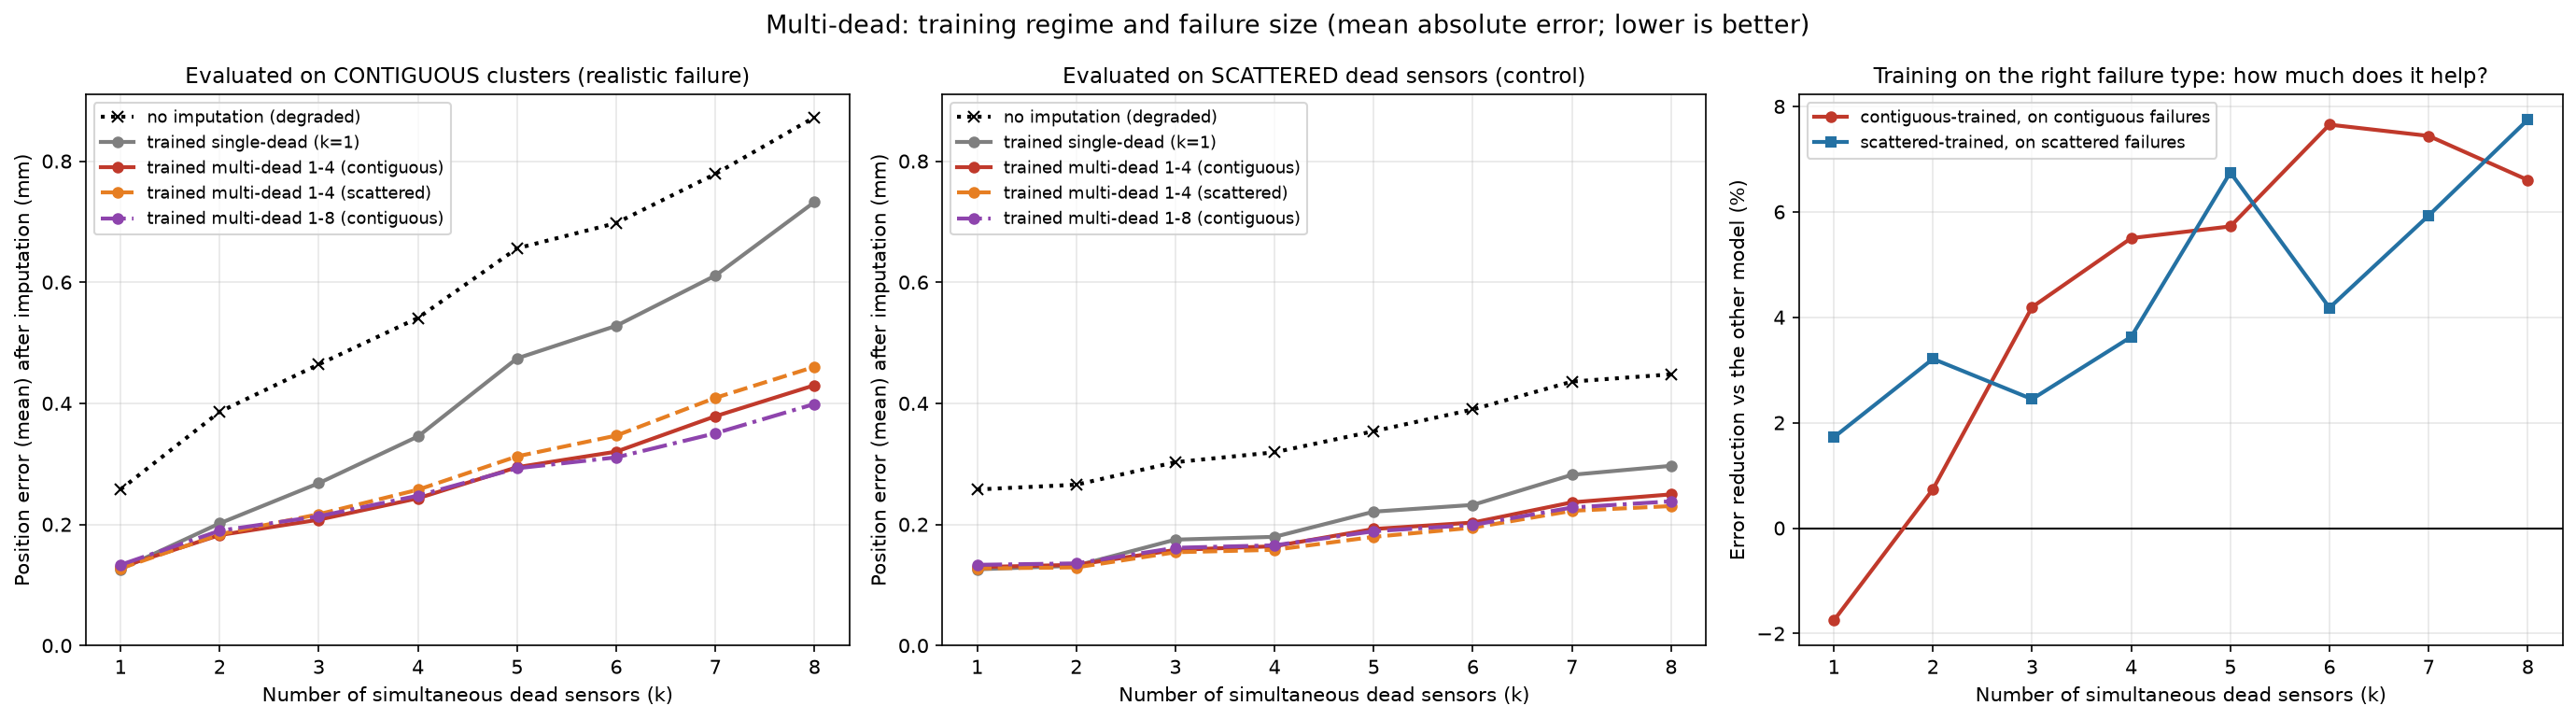
\includegraphics[width=\textwidth]{fig-multidead.png}
\caption{Error absoluto de posición tras la imputación en función del número de sensores averiados
simultáneamente, para los distintos regímenes de entrenamiento. El panel izquierdo corresponde a
fallos contiguos (caso realista) y el central a fallos dispersos (control); el panel derecho
cuantifica la ventaja de entrenar en el régimen que posteriormente se evalúa.}
\label{fig:multidead}
\end{figure}

Como referencia interpretativa, tras la imputación un fallo de ocho sensores contiguos ---el 13\,\%
del detector concentrado en una única región--- deja el módulo en una situación equivalente a la de
un fallo de dos sensores sin imputar, con un error muy inferior al paso entre sensores
(\SI{3.75}{\milli\metre}).

\subsection{Conservación del espectro de energía}
\label{subsec:res-espectro}

La Tabla~\ref{tab:res-espectro} presenta la recuperación espectral estratificada por zonas.

\begin{table}[htbp]
\centering
\caption{Recuperación espectral (\%) por zona del metahexágono y por sensor averiado,
modelo de referencia.}
\label{tab:res-espectro}
\begin{tabular}{lrrr}
\toprule
\textbf{Sensor averiado} & \textbf{Núcleo} & \textbf{Intermedia} & \textbf{Borde} \\
\midrule
$\mathrm{Ich}\,13$ (central) & 96.0 & 85.0 & 52.8 \\
$\mathrm{Ich}\,30$ (intermedio) & 78.6 & 88.7 & 91.7 \\
$\mathrm{Ich}\,32$ (mitad de lado) & 70.0 & 85.5 & 90.5 \\
$\mathrm{Ich}\,27$ (vértice) & 87.2 & 92.0 & 94.4 \\
$\mathrm{Ich}\,31$ (anómalo) & 84.3 & 70.4 & 76.5 \\
\midrule
\textbf{Media} & \textbf{83.2} & \textbf{84.3} & \textbf{81.2} \\
\bottomrule
\end{tabular}
\end{table}

La recuperación espectral se sitúa entre el 77\,\% y el 83\,\% según el sensor averiado, con un
residuo inferior al 0,5\,\% de la posición del fotopico. El resultado es \textbf{uniforme entre
zonas} (83,2 / 84,3 / 81,2), en contraste con la recuperación de posición, donde el borde sufre
apreciablemente más.

Esta disociación admite una interpretación física directa: la conservación de la energía requiere
únicamente acertar la \emph{magnitud} de la carga ausente, mientras que la reconstrucción de la
posición exige además que el \emph{reparto espacial} sea correcto. La estructura por sensor matiza
esta lectura: al enmascarar el sensor central y evaluar los eventos del borde, la recuperación cae
al 52,8\,\%, resultado esperable dado que dichos eventos apenas iluminan el centro del detector.

\subsection{Resolución espacial}
\label{subsec:res-resolucion}

La descomposición del error de posición en sesgo y dispersión arroja los resultados de la
Tabla~\ref{tab:res-resolucion}.

\begin{table}[htbp]
\centering
\caption{Descomposición del error de posición. Agregación macro sobre 61 canales.}
\label{tab:res-resolucion}
\begin{tabular}{lrrr}
\toprule
\textbf{Componente} & \textbf{Degradado} & \textbf{Imputado} & \textbf{Recuperación} \\
\midrule
Sesgo (mm) & 0.126 & 0.022 & 82.7\,\% \\
FWHM / dispersión (mm) & 0.166 & 0.085 & 48.8\,\% \\
\bottomrule
\end{tabular}
\end{table}

El contraste entre ambas componentes es informativo. El \textbf{sesgo se elimina casi por completo}
(82,7\,\%), lo que resulta esperable: el desplazamiento inducido por un canal ausente es sistemático
y por tanto predecible. La \textbf{dispersión se reduce únicamente a la mitad} (48,8\,\%), lo que
refleja el carácter irreducible de la incertidumbre evento a evento: el modelo puede estimar el
valor esperado de la carga ausente, pero no su realización concreta en un evento particular.

El análisis por canal revela que la recuperación mediana de la dispersión es del 51\,\%, con una cola
desfavorable: en dos o tres canales periféricos la mejora es marginal o incluso ligeramente negativa.

\subsection{Ensembles y descomposición sesgo-varianza}
\label{subsec:res-ensemble}

Ambos ensembles superan a la totalidad de sus miembros individuales
(Tabla~\ref{tab:res-ensemble}).

\begin{table}[htbp]
\centering
\caption{Rendimiento de los ensembles frente a la distribución de sus miembros.}
\label{tab:res-ensemble}
\begin{tabular}{lrrrr}
\toprule
\textbf{Configuración} & $\mathcal{R}_{\text{media}}$ & $\mathcal{R}_{p90}$ & \textbf{MAE} & $z$ ($\mathcal{R}_{\text{media}}$) \\
\midrule
Miembros (media $\pm$ desv.) & $52.32 \pm 0.35$ & $58.06 \pm 0.09$ & $0.6220 \pm 0.0026$ & --- \\
Ensemble homogéneo & 52.93 & 58.69 & \textbf{0.6110} & $+1.7$ \\
Ensemble heterogéneo & \textbf{53.21} & \textbf{58.73} & 0.6146 & $+2.5$ \\
\bottomrule
\end{tabular}
\end{table}

El ensemble heterogéneo supera al homogéneo en las métricas de posición, lo que establece que
\textbf{la diversidad arquitectónica aporta más que la diversidad de inicialización}. En el error de
carga, sin embargo, el homogéneo obtiene mejor resultado, lo que se atribuye a que el heterogéneo
incorpora miembros con peor rendimiento en dicha magnitud.

La lectura de mayor calado es la que corresponde a la descomposición sesgo-varianza. Si el error
estuviera dominado por la varianza entre entrenamientos, el promediado de tres modelos lo reduciría
en torno a un 40\,\%; si estuviera dominado por el límite de información, no lo alteraría. La
reducción observada es del \textbf{1,8\,\% en MAE}, de lo que se concluye que aproximadamente el
98\,\% del error es \textbf{irreducible} en el marco planteado.

\subsection{Estimación de incertidumbre}
\label{subsec:res-hetero}

El entrenamiento con la pérdida heterocedástica~\eqref{eq:nll} produjo una degradación severa:
$\mathcal{R}_{\text{media}} = 10.57$, MAE $= 1.31$ y error relativo del 63,2\,\%. La recuperación
mediana resultó \textbf{negativa} ($-18.16$), lo que indica que la imputación deja la posición en
peor situación que la ausencia de imputación.

La causa es un fallo conocido de la formulación: la pérdida~\eqref{eq:nll} permite al modelo reducir
el término cuadrático incrementando $\sigma$, pagando únicamente un coste logarítmico ---y por tanto
lineal en $\log\sigma$--- de modo que le resulta ventajoso sacrificar la precisión de $\mu$ a cambio
de declarar mayor incertidumbre. La corrección estándar consiste en un entrenamiento en dos fases,
con calentamiento bajo error cuadrático puro, o en el empleo de la formulación $\beta$-NLL. Se
documenta como línea de trabajo futuro.

\subsection{Cobertura del conjunto de entrenamiento}
\label{subsec:res-cobertura}

El experimento descrito en la Sección~\ref{subsec:exp-cobertura} arroja un resultado nítido y con
dos caras.

\begin{table}[htbp]
\centering
\caption{Efecto de entrenar con la totalidad de los módulos disponibles, a coste computacional
constante. Agregación macro sobre los 61 canales, \num{600000} eventos por fichero de test en ambos
casos.}
\label{tab:res-cobertura}
\small
\begin{tabular}{lrrr}
\toprule
\textbf{Magnitud} & \textbf{40 módulos} & \textbf{149 módulos} & \textbf{Diferencia} \\
\midrule
$\mathcal{R}_{p90}$ macro (\%) & 58.02 & 57.89 & $-0.13$ \\
$\mathcal{R}_{\text{media}}$ macro (\%) & 52.66 & 52.63 & $-0.02$ \\
$\mathcal{R}_{\text{mediana}}$ macro (\%) & 51.55 & 52.78 & $+1.23$ \\
MAE (ADC) & 0.620 & 0.616 & $-0.004$ \\
\midrule
Desviación entre canales (pts) & 4.49 & \textbf{3.77} & $-16\,\%$ \\
Recorrido entre canales (pts) & 25.2 & \textbf{15.4} & $-39\,\%$ \\
Peor canal (\%) & 38.6 & \textbf{47.9} & $\mathbf{+9.3}$ \\
Canal $\mathrm{Ich}\,31$ (\%) & 38.6 & \textbf{49.5} & $\mathbf{+11.0}$ \\
\bottomrule
\end{tabular}
\end{table}

\paragraph{En el rendimiento medio, ningún efecto.} La comparación pareada canal a canal arroja una
diferencia media de $-0.13$ puntos, con un estadístico $t = -0.49$ que no permite rechazar la
hipótesis nula, y solo 26 de los 61 canales mejoran, proporción indistinguible del azar. La
recuperación media queda en $52.63\,\%$, dentro de la banda de las réplicas
($52.32 \pm 0.35$). \textbf{El límite de rendimiento no procede de la cobertura del entrenamiento},
sino de la información físicamente disponible en los canales supervivientes. Este resultado
convierte en comprobación experimental directa lo que hasta ahora era una inferencia a partir de la
saturación de las distintas variantes arquitectónicas.

\paragraph{En la homogeneidad del detector, un efecto claro.} La dispersión entre canales se reduce
un $16\,\%$ y el recorrido entre el mejor y el peor sensor casi un $40\,\%$. El peor canal pasa de
$38.6\,\%$ a $47.9\,\%$, una mejora de $9.3$ puntos que, contrastada con la banda de las réplicas
para esa misma magnitud ($41.4 \pm 2.52$), corresponde a $z = +2.6$ y resulta por tanto
estadísticamente significativa.

\paragraph{Resolución del comportamiento anómalo de \texorpdfstring{$\mathrm{Ich}\,31$}{Ich 31}.}
Este canal, identificado sucesivamente como sensor defectuoso y como manifestación de la
variabilidad de ganancia entre módulos, mejora $11.0$ puntos al ampliar la cobertura. La
interpretación definitiva es que \textbf{los módulos de test en los que fallaba se encontraban fuera
del régimen estadístico representado en el entrenamiento}: no se trataba de un canal
intrínsecamente problemático, sino de una configuración de detector que el modelo nunca había
observado. Deja de constituir una anomalía del sensor para pasar a ser una manifestación medible de
la cobertura del conjunto de entrenamiento.

\paragraph{Conservación del espectro.} El efecto sobre la métrica energética apunta en la misma
dirección. La recuperación espectral media asciende de $82.9\,\%$ a $86.3\,\%$, y ---de nuevo lo más
relevante--- el peor caso mejora sustancialmente: la combinación más desfavorable, el canal central
evaluado sobre eventos de borde, pasa de $52.8\,\%$ a $65.8\,\%$. Nueve de las quince combinaciones
de canal y zona mejoran.

\paragraph{Resolución espacial y comparación con métodos clásicos.} Las dos magnitudes restantes se
mantienen sin cambios apreciables, lo que resulta coherente con la ausencia de efecto sobre el
rendimiento medio. La recuperación del emborronamiento mejora de forma marginal, de $48.8\,\%$ a
$49.5\,\%$, con una anchura a media altura residual prácticamente idéntica ($0.084$ frente a
$0.085$~mm) y una recuperación del sesgo equivalente ($82.6\,\%$ frente a $82.7\,\%$). La ventaja
sobre la regresión lineal, que sustenta la necesidad del aprendizaje profundo, se conserva en
$11.3$ puntos frente a los $11.5$ del modelo de referencia; la diferencia queda holgadamente dentro
de la variabilidad entre entrenamientos. Ninguno de los dos observables se ve por tanto perjudicado
por la ampliación de la cobertura.

\paragraph{Contrapartida: pérdida de robustez ante fallos múltiples.} La evaluación multi-dead
revela, sin embargo, un efecto de signo contrario que obliga a matizar la valoración. Ambos modelos
se entrenaron exclusivamente con un canal enmascarado, de modo que un fallo de dos o más sensores
constituye para ellos una situación no observada durante el entrenamiento. Con un único canal
averiado, el modelo de cobertura completa es superior, y de forma marcada en el peor caso
($45.9\,\%$ frente a $34.7\,\%$). Pero al aumentar el tamaño del fallo su rendimiento
\textbf{se desploma}: en agrupaciones contiguas de dos sensores la recuperación media cae a valores
negativos ---esto es, la imputación empeora la posición respecto a no imputar--- mientras que el
modelo de referencia se degrada de forma suave y conserva un $49.3\,\%$.

\begin{table}[htbp]
\centering
\caption{Recuperación media (\%) frente al tamaño del fallo, para dos modelos entrenados ambos con
un solo canal enmascarado. Valores negativos indican que la imputación desplaza la posición más de
lo que lo hace el propio fallo.}
\label{tab:res-cobertura-multidead}
\small
\begin{tabular}{lrrrr}
\toprule
\textbf{Modelo} & $k=1$ & $k=2$ & $k=3$ & $k=4$ \\
\midrule
\multicolumn{5}{l}{\emph{Agrupación contigua}} \\
\quad 40 módulos (referencia) & 51.39 & \textbf{49.28} & \textbf{44.21} & \textbf{37.59} \\
\quad 149 módulos & \textbf{51.64} & $-27.35$ & $-123.65$ & $-161.83$ \\
\midrule
\multicolumn{5}{l}{\emph{Fallo disperso}} \\
\quad 40 módulos (referencia) & 51.39 & \textbf{50.71} & \textbf{43.19} & \textbf{43.37} \\
\quad 149 módulos & \textbf{51.64} & 45.13 & 13.62 & $-3.96$ \\
\bottomrule
\end{tabular}
\end{table}

La interpretación más plausible es que el entrenamiento prolongado sobre un régimen de fallo único
---149 épocas frente a 40, con el punto de control seleccionado en la época 133--- produce una
función más ajustada a esa condición concreta y, por ello, más frágil fuera de la distribución de
entrenamiento. La cobertura completa mejora el caso para el que el modelo fue entrenado a costa de
su capacidad de extrapolación.

\paragraph{Implicación práctica.} Ampliar la cobertura no mejora el rendimiento promedio, pero
\textbf{homogeneiza la respuesta del detector sin coste computacional adicional}: eleva el peor
sensor nueve puntos y mejora la conservación del espectro. En un dispositivo real, donde la garantía
relevante es que ningún sensor se degrade de forma catastrófica, ese comportamiento resulta
preferible a una mejora marginal de la media. Ahora bien, la pérdida de robustez ante fallos
múltiples impide recomendar su adopción sin más: un modelo de producción con cobertura completa
debería entrenarse necesariamente en régimen multi-dead
(Sección~\ref{subsec:exp-multidead}), combinando ambas mejoras en lugar de intercambiarlas.

\subsection{Detección de canales defectuosos}
\label{subsec:res-bad}

La Tabla~\ref{tab:res-bad-roc} recoge la validación del estadístico de detección mediante inyección
de fallos con verdad conocida.

\begin{table}[htbp]
\centering
\caption{Validación del detector de canales defectuosos. Área bajo la curva ROC y tasas de
detección en el punto de operación.}
\label{tab:res-bad-roc}
\begin{tabular}{lrrr}
\toprule
\textbf{Severidad del fallo} & \textbf{AUC} & \textbf{TPR} ($Z=2.5$) & \textbf{FPR} \\
\midrule
100\,\% (canal muerto) & 1.000 & 1.000 & 0.009 \\
70\,\% & 0.998 & 0.952 & 0.009 \\
50\,\% & 0.973 & 0.422 & 0.009 \\
30\,\% & 0.868 & 0.091 & 0.009 \\
\bottomrule
\end{tabular}
\end{table}

El estadístico identifica los canales completamente inactivos con separación perfecta
($\mathrm{AUC} = 1.000$) y mantiene un rendimiento elevado para degradaciones severas. La tasa de
falsos positivos en los canales de borde resulta equivalente a la de los canales centrales, lo que
confirma que la normalización por canal resuelve efectivamente el problema del gradiente
estructural.

Las degradaciones moderadas, en cambio, no resultan separables en el punto de operación: si bien el
área bajo la curva indica que la información está presente, explotarla exigiría reducir el umbral y
asumir una tasa de falsos positivos considerablemente mayor.

\begin{figure}[htbp]
\centering
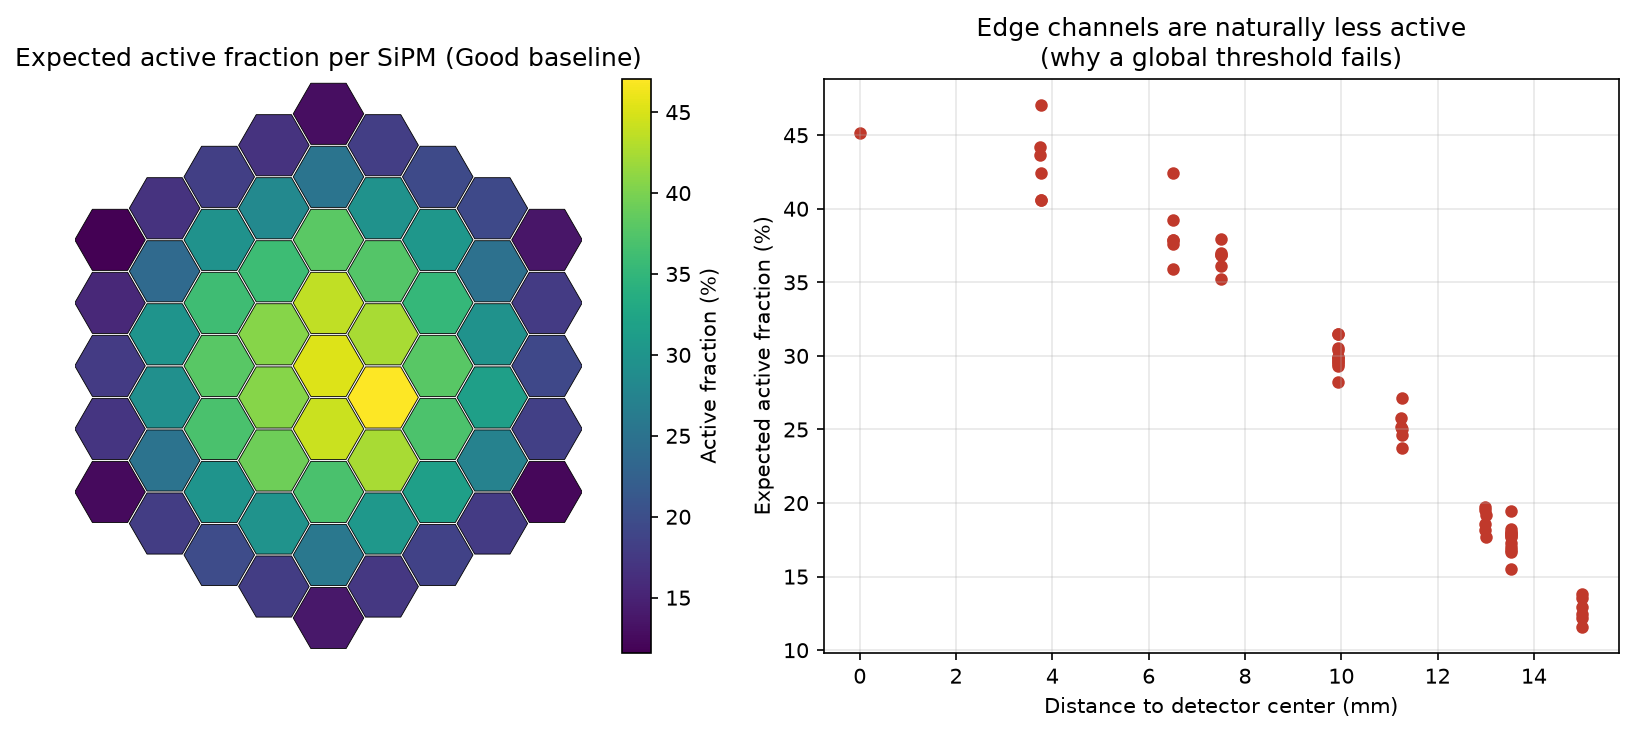
\includegraphics[width=0.95\textwidth]{fig-baseline-bad.png}
\caption{Actividad esperada por sensor en módulos sanos. Izquierda: mapa hexagonal del detector.
Derecha: dependencia con la distancia al centro, con una correlación de $-0.97$. Este gradiente
estructural es la razón por la que un umbral de detección global resulta inadecuado.}
\label{fig:baseline-bad}
\end{figure}

\begin{figure}[htbp]
\centering
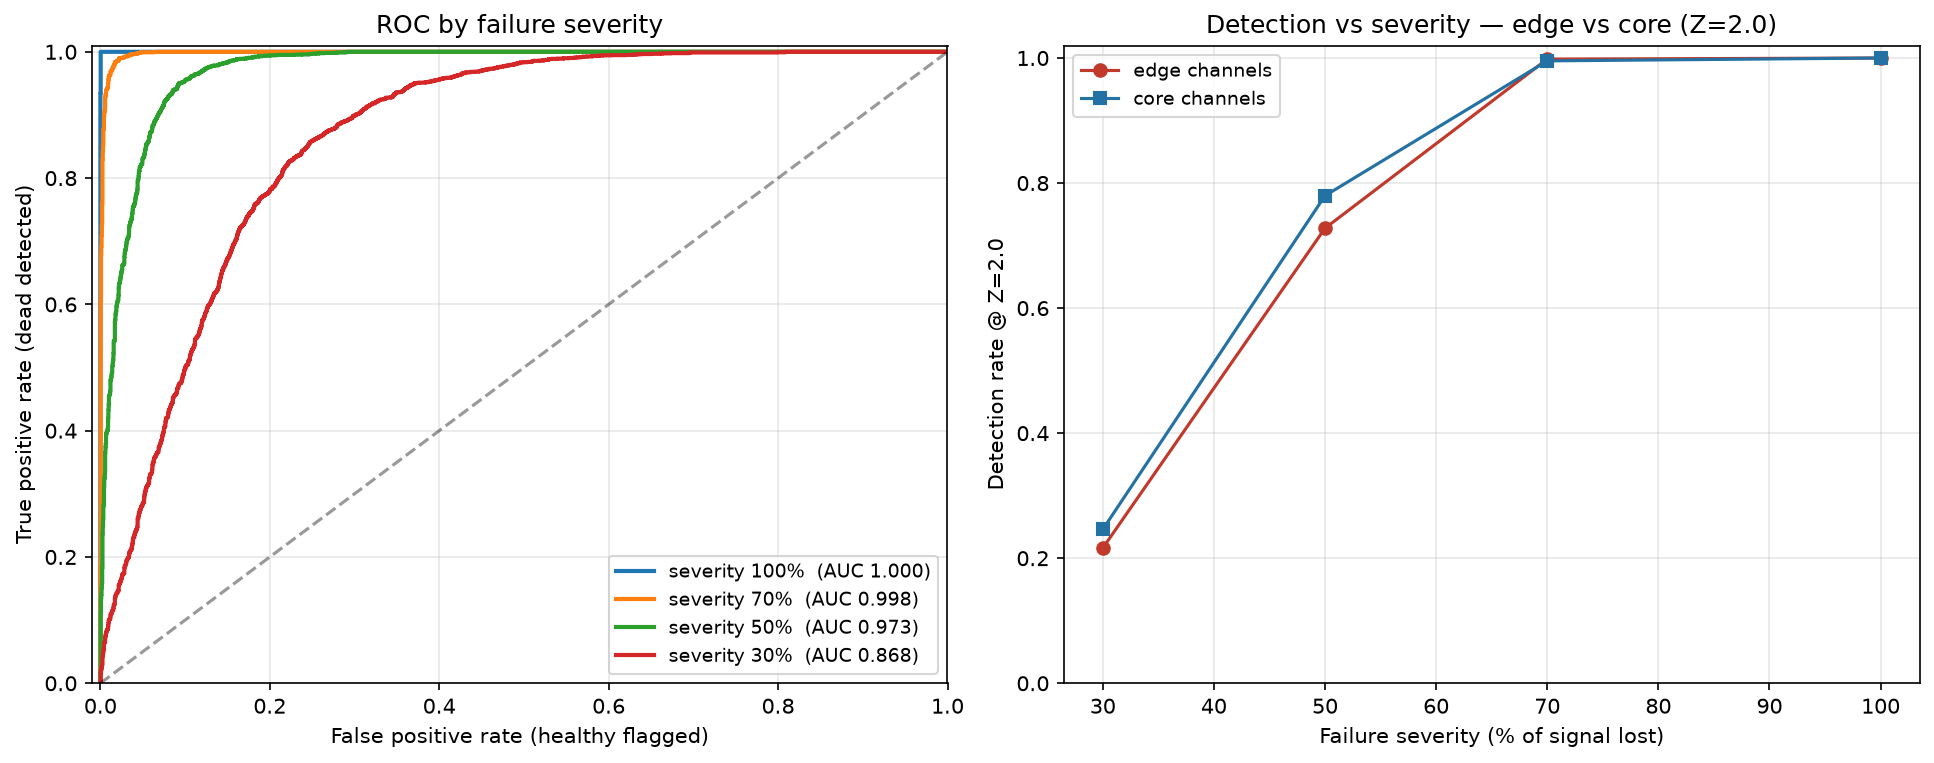
\includegraphics[width=0.95\textwidth]{fig-roc-bad.png}
\caption{Validación del estadístico de detección mediante inyección de fallos con verdad conocida.
Izquierda: curvas ROC para distintas severidades. Derecha: tasa de detección en el punto de
operación, desglosada entre canales de borde y centrales.}
\label{fig:roc-bad}
\end{figure}

Aplicado a los 62 módulos \textsc{Bad} con normalización por módulo y umbral $Z = 2.0$, el
procedimiento identifica canales defectuosos en \textbf{48} de los 62 módulos, marcando
\textbf{278} canales en total, y señala \textbf{12} módulos como globalmente desplazados.



\begin{figure}[htbp]
\centering
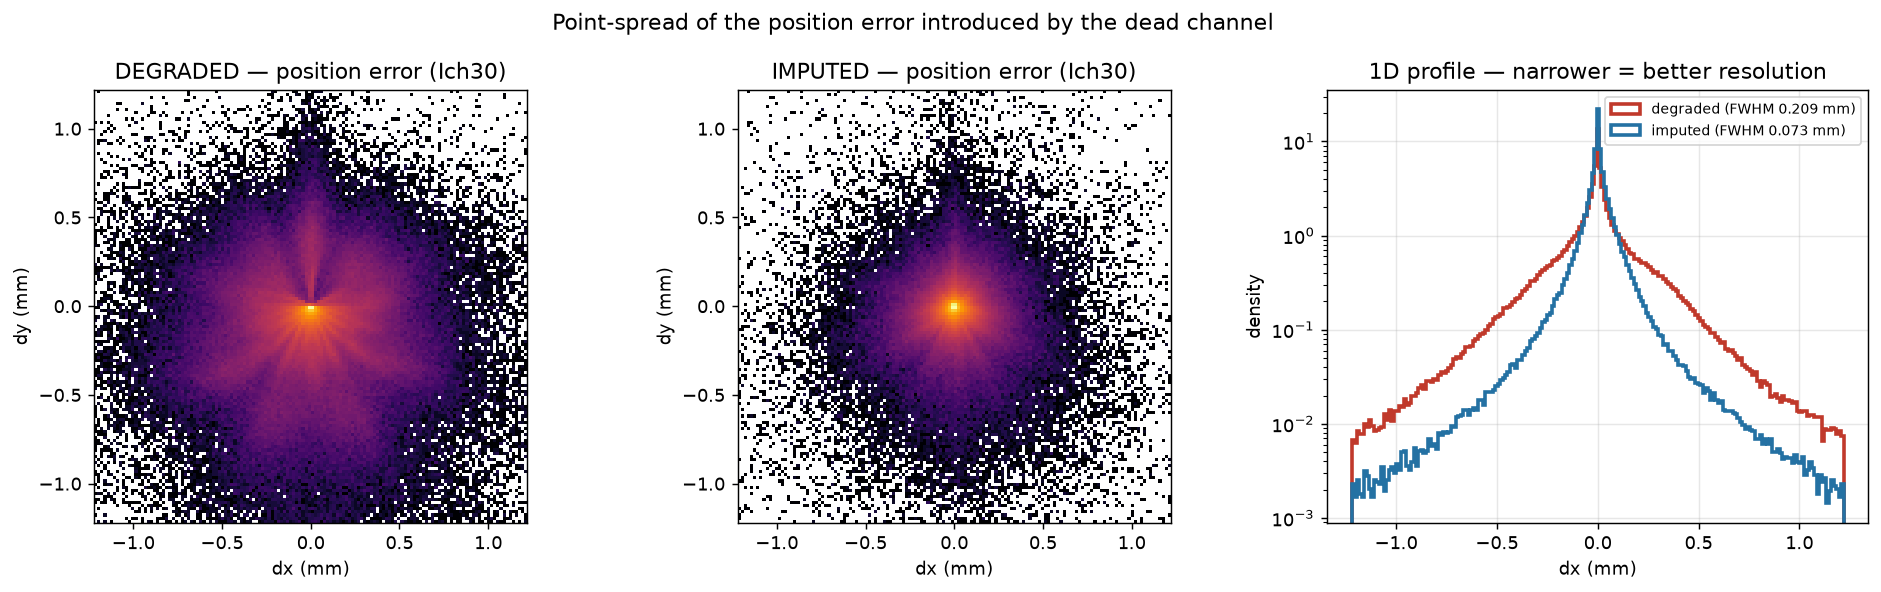
\includegraphics[width=0.95\textwidth]{fig-pointspread.png}
\caption{Distribución bidimensional del error de posición (\emph{point spread}) para el canal
$\mathrm{Ich}\,30$, antes y después de la imputación. La nube de la derecha es simultáneamente más
estrecha (menor dispersión) y está mejor centrada (menor sesgo) que la de la izquierda.}
\label{fig:pointspread}
\end{figure}

\begin{figure}[htbp]
\centering
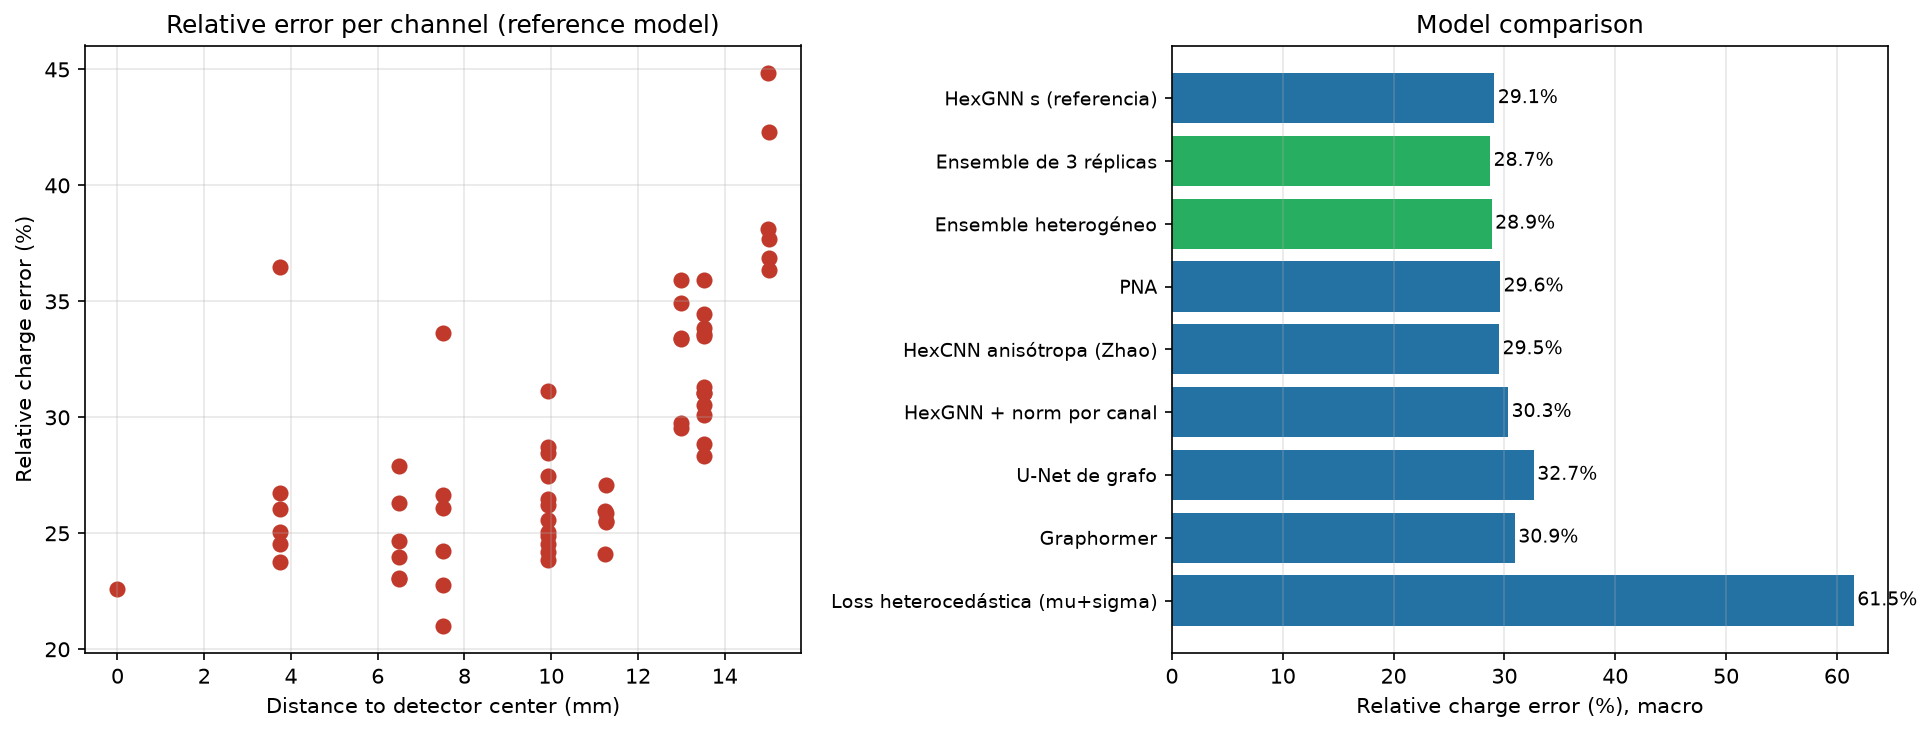
\includegraphics[width=0.95\textwidth]{fig-error-relativo.png}
\caption{Error relativo de carga. Izquierda: valor por canal frente a la distancia al centro del
detector, que evidencia el gradiente centro--borde. Derecha: comparación agregada entre las
configuraciones evaluadas.}
\label{fig:error-relativo}
\end{figure}

\section{Discusión}
\label{sec:discusion}

\subsection{Sobre la naturaleza del límite de rendimiento}

El conjunto de resultados converge de forma consistente hacia una conclusión: el rendimiento
alcanzado no está limitado por la arquitectura ni por la capacidad del modelo, sino por la
\textbf{información físicamente disponible} en los sensores operativos.

Esta conclusión se sustenta en cuatro evidencias independientes. En primer lugar, el incremento de
capacidad no mejora el rendimiento, e incluso lo degrada. En segundo lugar, diez variantes
arquitectónicas ---incluyendo transformadores, arquitecturas multiescala, agregadores múltiples y la
convolución hexagonal canónica--- no superan a la configuración de referencia. En tercer lugar, el
análisis por anillos demuestra que la información explotable se agota en el segundo anillo de
vecindad. Y en cuarto lugar, el ensemble ---que cancela la varianza entre entrenamientos--- recupera
únicamente un 1,8\,\% del error, lo que sitúa en torno al 98\,\% la fracción irreducible.

La descomposición del error de posición en sesgo y dispersión ofrece la interpretación física de
este límite. El sesgo, sistemático y por tanto predecible, se elimina casi por completo. La
dispersión, que corresponde a la incertidumbre sobre la realización concreta de la carga en cada
evento individual, solo se reduce a la mitad. Ninguna arquitectura puede eliminar esta segunda
componente, pues la información necesaria simplemente no está presente en los datos observados.

\subsection{Sobre la adecuación del diseño arquitectónico}

Los resultados permiten justificar el diseño adoptado desde tres perspectivas independientes.

La comparación con métodos clásicos establece que el aprendizaje profundo es \textbf{necesario}: la
red supera en 11,5 puntos a la regresión lineal. El análisis por anillos establece que la
información es \textbf{local}. Y la ablación del grafo establece que el prior geométrico es
\textbf{determinante}. En conjunto, estas tres evidencias caracterizan el modelo adecuado como uno
que sea simultáneamente local, no lineal e informado por la geometría del detector, que es
precisamente la descripción de la arquitectura propuesta.

El análisis de equivarianza añade una cuarta propiedad: la isotropía. La arquitectura respeta por
construcción la simetría $D_6$ del detector, propiedad que las variantes anisótropas rompen sin
obtener contrapartida, dado que el transporte de luz en el cristal es radialmente simétrico.

\subsection{Fortalezas del trabajo}

Cabe destacar como fortalezas metodológicas la definición de un marco de evaluación con significado
físico, que trasciende el error de reconstrucción y cuantifica el impacto sobre posición, energía y
resolución; el diseño diferencial emparejado para la evaluación espectral, que elimina la necesidad
de calibración previa; la estratificación mediante el metahexágono, físicamente motivada por la
geometría del absorbente; la inclusión sistemática de controles ---ablación del grafo, régimen
disperso, control de ruido en $k=1$, réplicas independientes--- que permiten atribuir causalmente los
efectos observados; y la cuantificación explícita de la variabilidad entre entrenamientos, que
proporciona el criterio para juzgar la significación de las comparaciones.

En el plano de los resultados, el hallazgo de que entrenar con fallos múltiples confiere robustez
sin coste alguno en el caso de un único canal tiene aplicabilidad práctica directa.

\subsection{Limitaciones}

\paragraph{Estadística de módulos reducida.} Conviene distinguir esta limitación de la cobertura del
entrenamiento tratada más abajo, con la que resulta fácil confundirla: aquella se refiere a
\emph{cuántos detectores ve el modelo} y afecta a lo que aprende; ésta se refiere a \emph{cuántos
detectores se emplean para medirlo} y afecta a la precisión de la métrica. Son independientes, y el
experimento de cobertura no resuelve la segunda.

La partición reserva únicamente cinco módulos para test. Aunque la estadística de eventos es holgada
---del orden de tres millones---, la de \emph{detectores} es pobre, de modo que las conclusiones
referidas a canales individuales pueden reflejar particularidades de esos cinco módulos concretos.
El caso del canal $\mathrm{Ich}\,31$ ilustra el problema: identificado inicialmente como canal
sistemáticamente anómalo, el análisis posterior reveló que su comportamiento en los módulos de
entrenamiento es normal y que la anomalía se concentra en dos módulos asignados a test; el
experimento de cobertura confirmó después que dichos módulos quedaban fuera del régimen estadístico
representado durante el entrenamiento.

La consecuencia metodológica es que las métricas agregadas carecen de una barra de error asociada al
\emph{efecto de módulo}: se dispone de la variabilidad entre entrenamientos
(Sección~\ref{subsec:res-replicas}), pero no de la variabilidad entre detectores. El procedimiento
descrito en el párrafo anterior ---evaluar sobre los 119 módulos no observados--- permite estimarla
sin reentrenar y se identifica como la comprobación pendiente de mayor valor.

\paragraph{Ausencia de validación cruzada.} No se ha realizado validación cruzada por módulos. La
razón no es el coste ---repetir el entrenamiento cinco veces es perfectamente asumible--- sino que
el número de hiperparámetros a ajustar es reducido y la selección del punto de control ya descansa
en un conjunto de validación independiente. Conviene, no obstante, precisar qué quedaría por
resolver: la validación cruzada no se necesitaría aquí para \emph{ajustar} nada, sino para
\textbf{acotar la sensibilidad de las métricas a qué cinco módulos concretos quedaron reservados
para test}, que es una cuestión distinta y sí pertinente.

Existe, además, una alternativa más económica y estadísticamente más potente que la validación
cruzada para esa pregunta concreta, derivada de la propia mecánica de rotación de ficheros. Puesto
que un modelo de 40 épocas solo llega a ver 40 de los 149 módulos de entrenamiento, los 109
restantes ---junto a los 5 de validación y los 5 de test--- constituyen \textbf{119 módulos que el
modelo no ha observado nunca}. Evaluar sobre ellos proporciona la dispersión entre detectores con
una estadística veinticuatro veces mayor que la del conjunto de test, y sin reentrenar. Es el
procedimiento recomendado para cerrar la limitación descrita en el párrafo siguiente.

\paragraph{Cobertura parcial del conjunto de entrenamiento.} El presupuesto de 40 épocas, combinado
con una rotación cíclica sobre la lista ordenada de ficheros, hace que el modelo utilice 40 de los
149 módulos disponibles, y que sean siempre los mismos. Como se detalla en la
Sección~\ref{subsec:carga-entrenamiento}, ese subconjunto resulta además más homogéneo que la
población completa. El experimento de la Sección~\ref{subsec:res-cobertura} demuestra que esta
limitación \textbf{no afecta al rendimiento medio} ---y por tanto no compromete ninguna de las
comparaciones entre modelos---, pero sí a la \emph{homogeneidad} entre canales: el protocolo de
producción subestima el peor caso en unos nueve puntos. Para trabajo posterior se recomienda adoptar
la cobertura completa, que no conlleva coste adicional.

\paragraph{Ausencia de calibración y filtrado en energía.} El conjunto incluye eventos Compton y de
fondo sin calibración de ganancia. Aunque el diseño diferencial cancela estos efectos en la
evaluación espectral, no puede descartarse que un conjunto calibrado y filtrado permitiera un
rendimiento superior.

\paragraph{Criterio de selección de modelo.} La métrica empleada para seleccionar el punto de
control no rastrea perfectamente el rendimiento en test, como se comprobó en el banco de pruebas.

\paragraph{Alcance del detector de canales defectuosos.} El estadístico desarrollado identifica de
forma fiable los canales inactivos, pero no separa las degradaciones moderadas de la variabilidad
normal, ni detecta canales con ganancia anómalamente elevada, dado que el estadístico es de una sola
cola. La distribución de puntuaciones en los módulos reales no presenta bimodalidad clara, lo que
indica que ``canal defectuoso'' no constituye una categoría con una firma estadística única sino un
conjunto heterogéneo de modos de fallo.

\paragraph{Ausencia de verdad de referencia en los módulos averiados.} La validación del detector se
apoya en fallos inyectados sobre módulos sanos, lo que garantiza una verdad conocida a costa de
evaluar un modo de fallo idealizado. En los módulos defectuosos reales no se dispone de anotación,
de modo que las detecciones no pueden contrastarse y el rendimiento medido no es directamente
extrapolable. La herramienta de etiquetado manual descrita en la Sección~\ref{subsec:exp-bad} se ha
desarrollado precisamente para levantar esta limitación; la anotación de los módulos y la medida del
acuerdo con el estadístico automático constituyen trabajo en curso.

\paragraph{Coste de inferencia del ensemble.} La mejor configuración identificada triplica el coste
de inferencia. Constituye por tanto una mejora en recursos y no en método, extremo que debe
explicitarse al reportar el resultado.

\subsection{Comparación entre aproximaciones}

La comparación entre familias arquitectónicas resulta ilustrativa. Los métodos sin estructura (MLP)
alcanzan recuperaciones del 48--51\,\%. Las arquitecturas basadas en paso de mensajes local se sitúan
en el rango 55--58\,\%. Las basadas en atención global obtienen 54--55\,\%, es decir, peor que las
locales pese a disponer de hasta cien veces más parámetros. La ordenación es coherente con la
naturaleza del problema: la estructura de grafo aporta, mientras que el contexto global no
únicamente no aporta sino que diluye la señal local relevante.

En cuanto a las estrategias de mejora ajenas a la arquitectura, se observa una asimetría notable:
mientras que ninguna modificación arquitectónica superó la referencia, el promediado de modelos sí
produjo una mejora estadísticamente significativa, aunque de magnitud modesta. Esto refuerza la
interpretación de que el margen de mejora disponible no reside en el diseño del modelo.


\section{Conclusiones preliminares}
\label{sec:conclusiones}

\subsection{Respuesta a los objetivos planteados}

\textbf{Sobre el diseño del modelo y el prior geométrico.} Se ha desarrollado una red neuronal de
grafos que explota la adyacencia física de los sensores, alcanzando una recuperación del error de
posición del 52--58\,\% con únicamente \num{38305} parámetros. La ablación del grafo establece de
forma concluyente que dicho prior es el elemento determinante del rendimiento: su eliminación reduce
la recuperación a la mitad.

\textbf{Sobre el marco de evaluación física.} Se ha desarrollado un conjunto de métricas que
cuantifican el impacto de la imputación sobre las tres magnitudes de interés. Los resultados indican
que el método recupera el 52--58\,\% del error de posición, el 77--83\,\% de la conservación del
espectro y el 48,8\,\% de la dispersión espacial, eliminando además el 82,7\,\% del sesgo
sistemático.

\textbf{Sobre la justificación del aprendizaje profundo.} La comparación con métodos clásicos
establece una ventaja de 11,5 puntos frente a la regresión lineal. El análisis por anillos precisa
el origen de dicha ventaja: no procede del acceso a información global ---que resulta irrelevante
más allá del segundo anillo--- sino de la capacidad de modelar relaciones no lineales.

\textbf{Sobre el límite del rendimiento.} El conjunto de evidencias establece que el rendimiento
está limitado por la información disponible y no por el modelo. La formulación de este resultado es
en sí misma una aportación: no se trata de que no se hayan encontrado arquitecturas mejores, sino de
que se ha caracterizado por qué la arquitectura adoptada es la adecuada.

\textbf{Sobre los fallos múltiples.} Entrenar con fallos múltiples contiguos reduce a la mitad el
error con ocho canales averiados, sin penalización alguna en el caso de un único canal, y
generalizando por encima del rango de entrenamiento. El régimen espacial del entrenamiento resulta
relevante, con una ventaja del 6--8\,\% frente a un nivel de ruido del 1,8\,\%.

\textbf{Sobre la detección de canales defectuosos.} Se ha desarrollado un estadístico que identifica
con separación perfecta los canales inactivos, resolviendo el problema del gradiente estructural
centro-borde. Su alcance queda limitado a los fallos severos.

\subsection{Contraste de las hipótesis planteadas}

De las hipótesis formuladas, se confirmaron la relativa al prior geométrico, la relativa a la
localidad de la información, la relativa al mayor daño de los fallos contiguos y la relativa al papel
del ensemble como estimador de la componente reducible del error.

Se refutaron, en cambio, las hipótesis relativas a la utilidad de las pérdidas physics-informed, al
beneficio de incorporar información direccional, a la ventaja de las arquitecturas de mayor
capacidad y a la conveniencia de la normalización por canal. Esta última merece comentario: la
hipótesis predecía una mejora en los canales periféricos, y el resultado fue una degradación
concentrada en los canales centrales. La explicación es que el estimador de posición pondera las
cargas cuadráticamente, de modo que los canales más brillantes dominan la magnitud de interés; la
pérdida cuadrática sin equalizar estaba, de forma no premeditada, alineada con esa ponderación, y
equalizar los canales rompe dicha alineación.

\subsection{Líneas de trabajo futuro}

Se identifican las siguientes líneas de continuación:

\begin{enumerate}
    \item \textbf{Estimación de incertidumbre con formulación corregida}, empleando entrenamiento en
    dos fases o la formulación $\beta$-NLL, con la finalidad de identificar y descartar los eventos
    cuya imputación resulte poco fiable.

    \item \textbf{Ampliación del estadístico de detección} mediante observables sensibles a la forma
    de la distribución de carga y con formulación de dos colas, que permitiría abordar los modos de
    fallo actualmente no cubiertos.

    \item \textbf{Combinación de cobertura completa y entrenamiento multi-canal.} Los resultados de
    la Sección~\ref{subsec:res-cobertura} muestran que ampliar la cobertura de módulos mejora la
    homogeneidad entre sensores y la conservación del espectro, pero degrada la extrapolación a
    fallos múltiples, mientras que el entrenamiento en régimen multi-canal
    (Sección~\ref{subsec:res-multidead}) proporciona precisamente esa robustez sin coste apreciable
    en el caso de fallo único. Al actuar sobre aspectos independientes del procedimiento, ambas
    intervenciones son en principio acumulables, y su combinación constituye la vía más directa
    hacia un modelo de producción que reúna las dos propiedades.

    \item \textbf{Anotación manual completa de los módulos averiados} con la herramienta descrita en
    la Sección~\ref{subsec:exp-bad}, que proporcionaría la verdad de referencia necesaria para medir
    el acuerdo entre el criterio experto y el estadístico automático sobre datos reales, y no
    únicamente sobre fallos inyectados.

    \item \textbf{Validación cruzada por módulos}, que permitiría acotar la sensibilidad de los
    resultados a la partición concreta y robustecer las conclusiones referidas a canales
    individuales.

    \item \textbf{Incorporación de la calibración en energía} y del filtrado correspondiente, con el
    fin de determinar si un conjunto de datos calibrado permite superar el límite observado.

    \item \textbf{Extensión a la corrección de canales anómalos}, generalizando el planteamiento
    desde la imputación de canales ausentes a la corrección de canales con respuesta alterada.

    \item \textbf{Evaluación del impacto sobre la imagen reconstruida}, cerrando la cadena desde la
    recuperación del módulo individual hasta la calidad de la imagen tomográfica final.
\end{enumerate}

% =====================================================================
%  MARCADORES PENDIENTES DE COMPLETAR
% =====================================================================
% TODO(1): Especificar el modelo concreto de SiPM, sus dimensiones activas y el
%          espesor del cristal LYSO. Esta información debe obtenerse de la
%          documentación del sistema experimental o del equipo del laboratorio.
% TODO(2): Detallar la actividad de la fuente de 22Na, la geometría de irradiación
%          y la duración de las adquisiciones.
% TODO(3): Especificar el modelo de ASIC empleado y el valor del umbral de
%          discriminación aplicado.
% TODO(5): Incluir las referencias bibliográficas correspondientes a: GraphSAGE
%          (Hamilton et al., 2017), PNA (Corso et al., 2020), Graphormer (Ying
%          et al., 2021), Graph U-Net (Gao y Ji, 2019), convolución hexagonal
%          (Zhao et al., 2021), beta-NLL (Seitzer et al., 2022), AdamW (Loshchilov
%          y Hutter, 2019) y modified z-score (Iglewicz y Hoaglin, 1993).
% TODO(6): Generar y enlazar las figuras marcadas como [FIGURA SUGERIDA].

\end{document}
.
% =====================================================================

\documentclass[11pt,a4paper]{report}

% ── Codificación e idioma ────────────────────────────────────────────
\usepackage[utf8]{inputenc}
\usepackage[T1]{fontenc}
\usepackage[spanish,es-tabla]{babel}
\usepackage{lmodern}
\usepackage{microtype}

% ── Matemáticas ──────────────────────────────────────────────────────
\usepackage{amsmath}
\usepackage{amssymb}

% ── Tablas y figuras ─────────────────────────────────────────────────
\usepackage{booktabs}
\usepackage{graphicx}
\usepackage{multirow}
\usepackage{siunitx}
\usepackage[font=small,labelfont=bf]{caption}
\usepackage{float}

% ── Formato de página ────────────────────────────────────────────────
\usepackage[a4paper,margin=2.7cm]{geometry}
\usepackage{setspace}
\onehalfspacing
\usepackage{fancyhdr}
\pagestyle{fancy}
\fancyhf{}
\fancyhead[L]{\small\nouppercase{\leftmark}}
\fancyhead[R]{\small\thepage}
\renewcommand{\headrulewidth}{0.4pt}

% ── Enlaces y referencias cruzadas ───────────────────────────────────
\usepackage[colorlinks=true,linkcolor=black,citecolor=black,urlcolor=blue]{hyperref}

% ── Configuración de siunitx (separador decimal español) ─────────────
\sisetup{
  output-decimal-marker = {.},
  group-separator = {\,},
  group-minimum-digits = 4,
  detect-weight = true,
  detect-family = true
}

% ── Ruta de las figuras ──────────────────────────────────────────────
\graphicspath{{figuras/}}

% =====================================================================

\title{%
    \vspace*{2cm}
    {\Huge\bfseries Materiales y métodos}\\[1.2cm]
    {\Large Imputación auto-supervisada de canales SiPM defectuosos\\
     en un detector PET de cristal monolítico hexagonal}\\[0.8cm]
    {\large Trabajo Fin de Máster}
}
\author{Miguel Escudero}
\date{\today}

\begin{document}

\maketitle
\tableofcontents
\listoftables
\listoffigures
\cleardoublepage

\chapter{Materiales y métodos}
\label{cap:materiales-metodos}

\section{Descripción del problema}
\label{sec:descripcion-problema}

\subsection{Contexto: detectores PET de cristal monolítico}
\label{subsec:contexto-pet}

La tomografía por emisión de positrones (PET) reconstruye la distribución espacial de un
radiotrazador emisor de positrones a partir de la detección en coincidencia de los dos fotones
de aniquilación de \SI{511}{\kilo\electronvolt} emitidos en direcciones opuestas. La calidad de
la imagen reconstruida depende de forma crítica de la precisión con que cada módulo detector
determina el punto de interacción del fotón incidente dentro del cristal centelleador.

Históricamente, los detectores PET han empleado matrices de cristales segmentados (\emph{pixelated
arrays}), en los que la posición de interacción se identifica con el cristal individual que
centellea. Esta aproximación desacopla la resolución espacial del proceso de reconstrucción, pero
impone un límite duro: la resolución no puede ser mejor que el tamaño del píxel, y la fracción de
material inactivo entre cristales (el \emph{dead space} de los separadores reflectantes) reduce la
sensibilidad efectiva del sistema.

Los detectores de \textbf{cristal monolítico} constituyen la alternativa que motiva este trabajo.
En ellos, un único bloque continuo de material centelleador ---en el sistema estudiado, un cristal
de ortosilicato de lutecio e itrio dopado con cerio (LYSO)--- se acopla ópticamente a una matriz
de fotomultiplicadores de silicio (SiPM). Cuando un fotón gamma interacciona en el interior del
cristal, la luz de centelleo se propaga isótropamente desde el punto de interacción y genera una
distribución de intensidad continua sobre el plano de sensores. La posición de interacción no se
lee directamente, sino que se \emph{estima} a partir del patrón de reparto de luz entre los
sensores. Esta estrategia elimina el material inactivo entre cristales, mejora la sensibilidad,
y permite en principio una resolución espacial superior al paso entre sensores, además de habilitar
la estimación de la profundidad de interacción (DOI). El precio a pagar es que la reconstrucción
de la posición deja de ser trivial y pasa a depender de un algoritmo de estimación.

El estimador clásico, y el empleado como referencia en este trabajo, es el
\textbf{centro de gravedad ponderado} (\emph{Anger logic}). Dadas las cargas $\{R_c\}_{c=1}^{N}$
registradas por los $N$ sensores situados en posiciones $\{(x_c, y_c)\}$, la posición estimada del
evento se calcula como

\begin{equation}
    \hat{x} = \frac{\sum_{c=1}^{N} R_c^{2}\, x_c}{\sum_{c=1}^{N} R_c^{2}},
    \qquad
    \hat{y} = \frac{\sum_{c=1}^{N} R_c^{2}\, y_c}{\sum_{c=1}^{N} R_c^{2}}.
    \label{eq:centroide}
\end{equation}

El exponente cuadrático sobre las cargas ---en lugar del centro de masas lineal--- concentra el
peso del estimador en los sensores más iluminados, lo que reduce la contribución de las colas de la
distribución de luz y mejora empíricamente la resolución en el interior del cristal. Nótese que la
expresión~\eqref{eq:centroide} es invariante frente a un reescalado global de las cargas
($R_c \rightarrow \alpha R_c$), propiedad que se explotará más adelante al normalizar los eventos.

La representación estándar de la respuesta de un detector monolítico es el \textbf{flood map}: el
histograma bidimensional de las posiciones $(\hat{x}, \hat{y})$ reconstruidas para un gran número de
eventos bajo irradiación uniforme. En un detector sano, el flood map presenta una estructura
característica que refleja tanto la geometría del cristal como la respuesta óptica del conjunto.

\subsection{El problema: canales SiPM defectuosos}
\label{subsec:problema-canales}

La expresión~\eqref{eq:centroide} pone de manifiesto la vulnerabilidad fundamental de los
detectores monolíticos: \textbf{la posición reconstruida depende simultáneamente de todos los
sensores}. Si un canal SiPM deja de funcionar ---y su carga registrada pasa a ser idénticamente
nula--- el numerador y el denominador del estimador se ven alterados de forma sistemática, y la
posición reconstruida se desplaza en dirección opuesta al sensor averiado. El efecto no es un ruido
aleatorio que se promedie a lo largo de la adquisición, sino un \textbf{sesgo estructural} que
distorsiona el flood map completo del módulo.

En un detector segmentado, la avería de un canal implica simplemente la pérdida del cristal
correspondiente: se degrada la sensibilidad, pero la posición de los eventos restantes no se ve
afectada. En un detector monolítico, en cambio, un único canal defectuoso contamina la
reconstrucción de \emph{todos} los eventos cuya distribución de luz alcanzaba a ese sensor. La
consecuencia práctica es que el módulo completo debe descartarse, sustituirse o recalibrarse, con el
coste asociado en tiempo de máquina y en disponibilidad del escáner.

Los modos de fallo observados en el sistema estudiado son heterogéneos. Se han identificado módulos
con un único canal completamente inactivo, módulos con bloques enteros del perímetro apagados
---compatibles con fallos de conexión en serie, sombras mecánicas o efectos térmicos localizados---
y canales que, sin estar muertos, presentan una ganancia anómala. Esta variedad condiciona el diseño
experimental descrito en la Sección~\ref{sec:experimentos}.

\subsection{Planteamiento como problema de imputación auto-supervisada}
\label{subsec:planteamiento}

La propuesta de este trabajo consiste en abordar la avería de un canal como un
\textbf{problema de imputación de datos faltantes}: dado el vector de cargas de los sensores
operativos, estimar la carga que \emph{habría} registrado el sensor averiado, de modo que la
expresión~\eqref{eq:centroide} pueda evaluarse sobre un vector completo y la posición reconstruida
recupere su valor correcto.

Formalmente, sea $\mathbf{R} = (R_1, \dots, R_N) \in \mathbb{R}_{\geq 0}^{N}$ el vector de cargas de
un evento y sea $\mathcal{D} \subset \{1,\dots,N\}$ el conjunto de canales averiados. Se busca una
función $f_\theta$ parametrizada por $\theta$ tal que

\begin{equation}
    \hat{R}_c = f_\theta\!\left(\mathbf{R}_{\setminus \mathcal{D}}, \mathcal{D}\right)_c
    \approx R_c
    \qquad \forall\, c \in \mathcal{D},
    \label{eq:problema-imputacion}
\end{equation}

donde $\mathbf{R}_{\setminus \mathcal{D}}$ denota el vector de cargas con los canales averiados
puestos a cero. La aproximación se juzga no por el error en la carga en sí, sino por su efecto sobre
la magnitud físicamente relevante: la posición reconstruida mediante~\eqref{eq:centroide}.

El aspecto metodológicamente central del planteamiento es su carácter
\textbf{auto-supervisado}. No se dispone de pares (entrada degradada, salida correcta) en los
módulos averiados reales, puesto que la carga verdadera del canal muerto es por definición
inobservable. Sin embargo, sí se dispone de un gran número de módulos \emph{sanos}, en los que es
posible \textbf{simular} la avería: se selecciona un canal, se fuerza su carga a cero, y se emplea
su valor original como etiqueta de supervisión. La supervisión, por tanto, se genera a partir de los
propios datos sin necesidad de anotación externa, lo que sitúa el enfoque en el paradigma del
aprendizaje auto-supervisado por enmascaramiento, análogo conceptualmente a los modelos de lenguaje
enmascarado o a los \emph{masked autoencoders} en visión por computador.

\paragraph{Fundamento físico de la imputabilidad.} Que el problema admita solución no resulta
evidente a priori y conviene justificarlo antes de describir el método. La luz de centelleo
generada por una interacción no se deposita sobre un único fotosensor: el cristal monolítico
reparte el destello sobre una vecindad de SiPM, de modo que la carga de cada canal constituye una
muestra local de una distribución de luz continua y extensa. La información asociada a un sensor
concreto se encuentra, por tanto, \textbf{parcialmente contenida en los sensores que lo rodean}, y
es precisamente esa redundancia la que hace posible reconstruir su valor. El tratamiento
superficial del cristal acota lateralmente la propagación de la luz y confina el destello a una
región de tamaño finito, lo que explica que la redundancia tenga carácter \emph{local}: los vecinos
inmediatos concentran la mayor parte de la información recuperable, mientras que los sensores
alejados apenas aportan. Esta observación anticipa un resultado experimental que se presenta más
adelante (Sección~\ref{subsec:res-anillos}) y motiva el diseño de una arquitectura basada en
vecindades.

Conviene precisar además en qué consiste realmente la tarea que aprende el modelo, pues la
formulación ingenua induce a error. La red no aprende una regla del tipo «si un sensor está apagado,
sustitúyase su valor»: aprende a evaluar si la carga observada en un canal resulta
\textbf{coherente con la distribución de luz que describen los canales restantes}. Para el cálculo
del centroide, por otra parte, no es el valor absoluto de carga de un SiPM lo determinante, sino el
modo en que la luz se reparte entre varios de ellos, lo que refuerza la decisión de normalizar por
evento discutida en la Sección~\ref{subsec:normalizacion}. Esta formulación tiene una consecuencia
práctica inmediata sobre el diseño del muestreo: el modelo debe aprender tanto a corregir cuando la
degradación altera la distribución de luz como a \textbf{abstenerse de corregir} cuando no la
altera, lo que fundamenta físicamente el esquema de balanceo descrito en la
Sección~\ref{subsec:generacion-muestras}.

\subsection{Objetivos}
\label{subsec:objetivos}

El objetivo general del trabajo es \emph{desarrollar y validar un método de imputación de canales
SiPM defectuosos en un detector PET de cristal monolítico que permita recuperar la calidad de
reconstrucción del módulo sin necesidad de sustituir el hardware}. Este objetivo se concreta en los
siguientes objetivos específicos:

\begin{enumerate}
    \item \textbf{Diseñar un modelo de imputación} que explote la estructura geométrica del
    detector, y caracterizar en qué medida dicho prior geométrico contribuye al rendimiento.

    \item \textbf{Establecer el marco de evaluación física} adecuado, que no se limite al error de
    reconstrucción de la carga sino que cuantifique el impacto sobre las magnitudes de interés en
    PET: la posición reconstruida, el espectro de energía y la resolución espacial.

    \item \textbf{Determinar si el aprendizaje profundo está justificado} frente a alternativas
    clásicas de menor complejidad, mediante una comparación rigurosa con métodos de interpolación
    y regresión lineal.

    \item \textbf{Explorar el espacio de arquitecturas} para establecer si el rendimiento obtenido
    está limitado por la capacidad del modelo o por la información físicamente disponible.

    \item \textbf{Extender el método al caso de múltiples canales averiados simultáneamente},
    con especial atención a la configuración físicamente realista de fallos contiguos.

    \item \textbf{Desarrollar un procedimiento de detección} de canales defectuosos que permita
    aplicar el método sobre módulos reales no etiquetados.
\end{enumerate}


\section{Materiales}
\label{sec:materiales}

\subsection{Sistema detector}
\label{subsec:sistema-detector}

El sistema experimental del que proceden los datos consiste en módulos detectores basados en un
cristal centelleador monolítico de LYSO de geometría hexagonal, acoplado a una matriz de SiPM
dispuestos en una retícula hexagonal. La lectura se realiza mediante un circuito integrado de
aplicación específica (ASIC) que digitaliza la carga integrada por cada canal y aplica un umbral de
discriminación para suprimir el ruido electrónico.

La matriz de fotosensores consta de \textbf{64 canales} de lectura, de los cuales \textbf{61 se
encuentran físicamente instrumentados}; los canales con identificadores $\mathrm{Ich} \in
\{1, 16, 18\}$ no disponen de SiPM asociado y se excluyen sistemáticamente del análisis. En lo
sucesivo se emplea una indexación densa $i \in \{0, \dots, 60\}$ sobre los canales activos, junto
con las tablas de conversión correspondientes al identificador físico $\mathrm{Ich}$.

Las posiciones físicas de los 61 sensores se obtienen del fichero de configuración
\texttt{psipm.tsv}. La caracterización geométrica derivada de dichas posiciones se resume en la
Tabla~\ref{tab:geometria-detector}. Cabe destacar que el paso entre sensores vecinos
(\emph{pitch}) es de \SI{3.75}{\milli\metre}, valor que constituye la escala natural de referencia
para interpretar los errores de posición reportados en la Sección~\ref{sec:resultados}.

\begin{table}[htbp]
\centering
\caption{Caracterización geométrica del módulo detector, obtenida de las posiciones físicas
de los sensores.}
\label{tab:geometria-detector}
\begin{tabular}{lc}
\toprule
\textbf{Magnitud} & \textbf{Valor} \\
\midrule
Canales de lectura totales & 64 \\
Canales instrumentados (activos) & 61 \\
Canales inactivos ($\mathrm{Ich}$) & 1, 16, 18 \\
Paso entre sensores vecinos (\emph{pitch}) & \SI{3.75}{\milli\metre} \\
Extensión en $x$ & $[-13.0,\ 13.0]$~mm \\
Extensión en $y$ & $[-15.0,\ 15.0]$~mm \\
Radio máximo desde el centro & \SI{15.01}{\milli\metre} \\
Geometría de la retícula & Hexagonal (hexágono de lado 5) \\
\bottomrule
\end{tabular}
\end{table}

Un aspecto físico determinante para la interpretación de los resultados es la presencia de un
\textbf{adhesivo absorbente (negro) en las caras laterales del cristal}. Su función es suprimir las
reflexiones en los bordes, que de otro modo degradarían la estimación de posición, pero tiene como
efecto colateral que los eventos que interaccionan cerca del perímetro pierden una fracción
significativa de la luz de centelleo. Este hecho, confirmado por el análisis de los datos, se
traduce en dos observaciones recurrentes a lo largo del trabajo: los sensores del borde registran
sistemáticamente menos carga que los centrales, y el fotopico de energía se desplaza hacia energías
menores en las regiones periféricas del cristal.

\begin{figure}[htbp]
\centering
% \includegraphics[width=0.6\textwidth]{figuras/geometria_detector.pdf}
\caption{\textbf{[FIGURA SUGERIDA]} Disposición de los 61 SiPM activos sobre el plano del detector,
con la retícula hexagonal y la numeración $\mathrm{Ich}$ de cada canal. Se recomienda superponer el
contorno del cristal y señalar la posición del adhesivo absorbente en las caras laterales.}
\label{fig:geometria-detector}
\end{figure}

\subsection{Entorno software}
\label{subsec:entorno-software}

La totalidad del desarrollo se ha realizado en Python sobre un entorno gestionado con
\texttt{conda}. La Tabla~\ref{tab:entorno-software} recoge las versiones exactas de los componentes
empleados, información necesaria para garantizar la reproducibilidad de los experimentos.

\begin{table}[htbp]
\centering
\caption{Entorno software y hardware empleado en el desarrollo y la experimentación.}
\label{tab:entorno-software}
\begin{tabular}{lll}
\toprule
\textbf{Componente} & \textbf{Versión} & \textbf{Función en el trabajo} \\
\midrule
Python & 3.11.15 & Lenguaje de implementación \\
PyTorch & 2.5.1+cu121 & Definición y entrenamiento de los modelos \\
CUDA & 12.1 & Aceleración por GPU \\
NumPy & 2.4.4 & Álgebra y manipulación de arrays \\
SciPy & 1.17.1 & \texttt{cKDTree}, \texttt{ConvexHull}, distancia de Wasserstein \\
Matplotlib & 3.11.0 & Generación de figuras \\
openpyxl & 3.1.5 & Exportación de tablas de métricas \\
Weights \& Biases & 0.28.0 & Registro y trazabilidad de experimentos \\
\midrule
GPU & NVIDIA GTX 1660 SUPER & Entrenamiento e inferencia \\
Sistema operativo & Windows 11 & Entorno de ejecución \\
\bottomrule
\end{tabular}
\end{table}

La elección de PyTorch como \emph{framework} responde a la necesidad de implementar operadores de
paso de mensajes sobre un grafo con topología fija y no estándar. Aunque existen bibliotecas
especializadas en redes de grafos (\texttt{PyTorch Geometric}, \texttt{DGL}), se optó
deliberadamente por una implementación directa con tensores densos. Esta decisión se justifica por
tres motivos: el grafo del detector es pequeño ($N = 61$ nodos) y \emph{fijo}, lo que hace que la
indexación densa sea más eficiente que las estructuras dispersas generales; se elimina una
dependencia externa cuyo ciclo de versiones es sensible a la de PyTorch; y, sobre todo, se mantiene
control explícito sobre la operación de agregación, aspecto que resulta central en los experimentos
de la Sección~\ref{sec:experimentos}.

\subsection{Herramientas de desarrollo y trazabilidad}
\label{subsec:herramientas}

El control de versiones del código se ha realizado con Git, sobre un repositorio alojado en GitHub.
El seguimiento de los experimentos de entrenamiento y evaluación se ha llevado a cabo con
Weights~\&~Biases, registrando de forma sistemática los hiperparámetros, las curvas de entrenamiento
y las figuras resultantes de cada evaluación. Los procesos de entrenamiento y evaluación se
registran como ejecuciones diferenciadas mediante el campo \texttt{job\_type}, lo que permite
trazar qué evaluación corresponde a qué modelo.

Adicionalmente, se ha mantenido un cuaderno de laboratorio en formato Markdown en el que se han
documentado de forma cronológica las decisiones metodológicas, los resultados obtenidos y ---de
manera explícita--- las hipótesis descartadas y los errores de interpretación detectados y
corregidos. Esta práctica ha resultado determinante para la coherencia del trabajo, dado el elevado
número de experimentos realizados.

\subsection{Organización del código}
\label{subsec:organizacion-codigo}

La implementación se estructura en módulos con responsabilidades bien delimitadas, cuya
descripción funcional se recoge en la Tabla~\ref{tab:modulos-codigo}. El diseño responde al
principio de \emph{fuente única de verdad}: elementos críticos como la partición de los datos o la
construcción del grafo de vecindad se definen en un único lugar y son importados por el resto de
módulos, de modo que resulta imposible que el entrenamiento y la evaluación operen sobre
configuraciones discrepantes.

\begin{table}[htbp]
\centering
\caption{Módulos principales de la implementación y su responsabilidad.}
\label{tab:modulos-codigo}
\small
\begin{tabular}{p{0.26\textwidth}p{0.66\textwidth}}
\toprule
\textbf{Módulo} & \textbf{Responsabilidad} \\
\midrule
\texttt{dataset.py} & Lectura del formato binario, densificación, generación de muestras
    auto-supervisadas \emph{on-the-fly} y partición reproducible de los ficheros. \\
\texttt{hex\_geometry.py} & Construcción del grafo de vecindad, vectores de arista, matriz de
    vecindad direccional y escala característica por canal. \\
\texttt{model.py} & Definición de las arquitecturas de producción y del ensemble. \\
\texttt{train.py} & Bucle de entrenamiento, funciones de pérdida y selección de modelo. \\
\texttt{imputation\_eval.py} & Carga de modelos, rutina de imputación y evaluación monocanal. \\
\texttt{eval\_total.py} & Evaluación multicanal sobre los 61 sensores y análisis por líneas. \\
\texttt{eval\_espectro.py} & Conservación del espectro de energía estratificada por zonas. \\
\texttt{eval\_multidead.py} & Barrido de tamaño de fallo y régimen espacial. \\
\texttt{eval\_resolution.py} & Descomposición del error de posición en sesgo y dispersión. \\
\texttt{eval\_baselines.py} & Comparación con métodos clásicos. \\
\texttt{eval\_linear\_rings.py} & Análisis de localidad de la información mediante regresión por anillos. \\
\texttt{sandbox\_arch*.py} & Banco de pruebas de arquitecturas alternativas. \\
\texttt{bad\_detect.py} & Estadístico de detección de canales defectuosos. \\
\texttt{bad\_validate.py} & Validación del detector con verdad conocida por inyección. \\
\texttt{bad\_label.py} & Interfaz de etiquetado manual asistido de los módulos averiados. \\
\bottomrule
\end{tabular}
\end{table}


\section{Conjunto de datos}
\label{sec:datos}

\subsection{Origen y naturaleza de los datos}
\label{subsec:origen-datos}

Los datos proceden de adquisiciones experimentales realizadas sobre módulos detectores irradiados
con una fuente de $^{22}$Na. Este isótopo es un emisor de positrones cuyo espectro de energía
presenta dos líneas características: el fotopico de aniquilación a \SI{511}{\kilo\electronvolt} y
una segunda línea a \SI{1275}{\kilo\electronvolt} procedente de la desexcitación del núcleo hijo.
La presencia de estas líneas en el espectro de energía reconstruido se ha empleado como control de
calidad de los datos.

Es importante señalar que las adquisiciones se registran en modo \emph{singles}, es decir, cada
evento se almacena sin aplicar filtro de coincidencia. Esto implica que el conjunto contiene tanto
eventos de fotopico como eventos de dispersión Compton y sucesos de fondo, lo que amplía el rango
dinámico de las cargas registradas y constituye un factor a considerar en la interpretación de los
espectros.

El conjunto de datos se organiza en dos poblaciones diferenciadas:

\begin{itemize}
    \item \textbf{Módulos \textsc{Good}}: \textbf{159 ficheros}, correspondientes a módulos cuyos
    61 canales se consideran operativos. Constituyen la base para el entrenamiento y para toda la
    evaluación con verdad de referencia conocida.

    \item \textbf{Módulos \textsc{Bad}}: \textbf{62 ficheros}, correspondientes a módulos con uno o
    más canales defectuosos. No disponen de etiquetado: se desconoce a priori qué canales fallan y
    en qué grado. Se emplean exclusivamente en la fase de aplicación y validación cualitativa
    (Sección~\ref{subsec:exp-bad}).
\end{itemize}

Cada fichero corresponde a un módulo físico distinto del escáner, con un volumen medio de
\SI{161}{\mega\byte} y del orden de $10^6$ eventos. El volumen total del conjunto \textsc{Good}
asciende aproximadamente a \SI{25.5}{\giga\byte}, magnitud que ha condicionado de forma directa la
estrategia de carga de datos descrita en la Sección~\ref{subsec:generacion-muestras}.

\subsection{Formato binario y lectura}
\label{subsec:formato-binario}

Los ficheros \texttt{.dat} emplean un formato binario compacto de longitud variable por evento,
diseñado para almacenar únicamente los canales que superan el umbral del ASIC. La estructura de
cada evento es la siguiente:

\begin{enumerate}
    \item Un byte sin signo, $N_{\text{int}}$, que indica el número de canales que han registrado
    señal en el evento.
    \item A continuación, $N_{\text{int}}$ registros consecutivos de 8 bytes, cada uno compuesto por
    un valor de carga en coma flotante de precisión simple (\texttt{float32}, \emph{little-endian})
    seguido del identificador de canal como entero de 32 bits (\texttt{int32}).
\end{enumerate}

La lectura se implementa cargando el fichero completo en memoria y recorriéndolo mediante una vista
sin copia (\texttt{memoryview}), interpretando cada bloque de registros con
\texttt{numpy.frombuffer} sobre un \texttt{dtype} estructurado. Esta estrategia evita el
procesamiento byte a byte en Python, que resultaría prohibitivo para conjuntos de millones de
eventos.

El resultado de la lectura es la \textbf{densificación} del evento: el formato disperso
$(R_c, \mathrm{Ich}_c)$ se convierte en un vector denso de dimensión 61, en el que los canales que no
superaron el umbral toman valor cero. Esta representación densa y de dimensión fija es la que
consume el modelo.

Conviene subrayar que la \emph{sparsity} observada ---en promedio, únicamente \textbf{17 de los 61
canales} registran señal en un evento dado--- no constituye un defecto de los datos ni una pérdida
de información recuperable, sino el comportamiento nominal del sistema: el ASIC aplica un umbral de
discriminación para suprimir el ruido electrónico térmico, de modo que un canal a cero indica que el
sistema de adquisición ya determinó que no había señal significativa. Esta interpretación es
relevante porque justifica la definición de la etiqueta interna descrita en la
Sección~\ref{subsec:generacion-muestras}.

\subsection{Caracterización estadística}
\label{subsec:caracterizacion-datos}

La Tabla~\ref{tab:caracterizacion-datos} resume las propiedades estadísticas del conjunto,
obtenidas sobre los ficheros de la partición de test.

\begin{table}[htbp]
\centering
\caption{Caracterización estadística del conjunto de datos.}
\label{tab:caracterizacion-datos}
\begin{tabular}{lc}
\toprule
\textbf{Magnitud} & \textbf{Valor} \\
\midrule
Ficheros \textsc{Good} & 159 \\
Ficheros \textsc{Bad} & 62 \\
Tamaño medio por fichero & \SI{161}{\mega\byte} \\
Volumen total (\textsc{Good}) & \SI{25.5}{\giga\byte} \\
Eventos por fichero (orden de magnitud) & $\sim 10^6$ \\
Eventos totales en la partición de test & \num{5476642} \\
Canales activos por evento (media) & 17.0 \\
Canales activos por evento (rango) & 1--54 \\
Carga total por evento, $R_T$ (media) & 31.9 (ADC) \\
Carga total por evento, $R_T$ (mediana) & 26.8 (ADC) \\
\bottomrule
\end{tabular}
\end{table}

La diferencia entre la media y la mediana de la carga total por evento ($31.9$ frente a $26.8$)
evidencia la asimetría de la distribución de energía, consistente con la presencia de una cola de
eventos de alta energía sobre un fondo Compton dominante.

\subsection{Limpieza y preprocesado}
\label{subsec:preprocesado}

El preprocesado aplicado ha sido deliberadamente mínimo, con el fin de evitar la introducción de
sesgos no controlados. Las operaciones realizadas, y su justificación, son las siguientes.

\paragraph{Tratamiento de cargas negativas.} Una fracción de los valores de carga registrados es
negativa. Estos valores no corresponden a señal física, sino a artefactos de la cadena de lectura:
parámetros de calibración que no ajustan correctamente el rango dinámico del ADC, o errores de
conexión. Se aplica un recorte a cero,
\begin{equation}
    R_c \leftarrow \max(R_c, 0),
\end{equation}
en lugar del valor absoluto. Esta elección, validada con el equipo experimental, es la
metodológicamente correcta: tomar el valor absoluto \emph{inventaría} señal donde no la hay,
mientras que el recorte se limita a reconocer la ausencia de señal significativa.

\paragraph{Descarte de eventos vacíos.} Se eliminan los eventos cuya carga total resulta nula tras
el recorte. Estos sucesos no aportan información y, además, provocarían una división por cero en la
normalización descrita más adelante.

\paragraph{Ausencia de filtrado en energía.} Se ha decidido \textbf{no} aplicar ningún filtro de
selección en energía (por ejemplo, una ventana en torno al fotopico de \SI{511}{\kilo\electronvolt}).
La justificación es doble. En primer lugar, un filtrado riguroso requeriría una calibración en
energía previa ---la alineación de los fotopicos canal a canal--- que no está disponible y cuya
obtención excede el alcance del trabajo. En segundo lugar, el filtrado reduciría sustancialmente el
tamaño del conjunto de entrenamiento sin una ventaja clara: el objetivo del modelo es reconstruir la
carga de un canal a partir de los restantes, tarea que no depende de que el evento pertenezca al
fotopico. Se documenta, no obstante, como limitación en la Sección~\ref{sec:discusion}.

\paragraph{Ausencia de calibración en energía.} Por el mismo motivo, no se ha aplicado corrección de
ganancia canal a canal. Esta decisión tiene una implicación metodológica importante que se ha
explotado deliberadamente en el diseño de la evaluación del espectro
(Sección~\ref{subsec:met-espectro}): al emplear un diseño \emph{diferencial emparejado} sobre los
mismos eventos, los efectos de la falta de calibración se cancelan y no contaminan la métrica.

\subsection{Normalización por evento}
\label{subsec:normalizacion}

Cada muestra se normaliza dividiendo el vector de cargas por un factor de escala calculado
\textbf{a nivel de evento} y, de forma crítica, \textbf{después} de aplicar el enmascaramiento:

\begin{equation}
    \eta = \max_{c \notin \mathcal{D}} R_c,
    \qquad
    \mathbf{x}^{\text{in}} = \frac{\mathbf{R}_{\setminus \mathcal{D}}}{\eta},
    \qquad
    \mathbf{y}^{\text{target}} = \frac{\mathbf{R}}{\eta}.
    \label{eq:normalizacion}
\end{equation}

La normalización por evento fue recomendada por el equipo experimental con el fin de evitar
oscilaciones en el entrenamiento derivadas de las variaciones de calibración entre módulos. Su
fundamento físico es que la información relevante para localizar el punto de interacción reside en
la \emph{distribución relativa} de la luz entre sensores, no en su magnitud absoluta; obsérvese que
el estimador~\eqref{eq:centroide} es efectivamente invariante a esta escala.

Dos consecuencias del esquema~\eqref{eq:normalizacion} merecen comentario explícito:

\begin{itemize}
    \item \textbf{Entrada y objetivo comparten el mismo factor $\eta$.} Esto es necesario para que
    la predicción sea reescalable a unidades físicas, pero implica que si el canal enmascarado era el
    más brillante del evento, entonces $y^{\text{target}}_c > 1$. Por este motivo la salida de todas
    las redes es \textbf{estrictamente lineal}, sin función de activación acotante (sigmoide o
    recorte) en la última capa: acotar la salida haría imposible predecir correctamente esos casos.

    \item \textbf{El factor depende de un único canal.} Al emplear el máximo, la escala del evento
    queda determinada por el sensor más iluminado. Esta dependencia se identificó como una posible
    fuente de fragilidad y motivó el experimento descrito en la Sección~\ref{subsec:exp-norm}, en el
    que se evaluó una normalización alternativa basada en la suma.
\end{itemize}

\subsection{Generación de muestras auto-supervisadas}
\label{subsec:generacion-muestras}

La generación de las muestras de entrenamiento se realiza \textbf{al vuelo} (\emph{on-the-fly}),
sin materializar en disco el conjunto de pares (entrada, objetivo). La razón es dimensional: con
$\sim 10^6$ eventos por fichero, 159 ficheros y 61 posibles canales a enmascarar por evento, el
conjunto completo de muestras posibles sería del orden de $10^{10}$, inviable de almacenar. La
generación dinámica permite además que el enmascaramiento cambie en cada época, lo que actúa como
una forma natural de aumento de datos.

El procedimiento para cada muestra es el siguiente:

\begin{enumerate}
    \item Se toma un evento sano $\mathbf{R}$ del fichero cargado en la época actual.
    \item Se selecciona el canal (o conjunto de canales) a enmascarar según la política de balanceo
    descrita a continuación.
    \item Se anula la carga de dichos canales y se normaliza según~\eqref{eq:normalizacion}.
    \item Se construye la entrada como una matriz de dos filas y 61 columnas: la primera contiene
    las cargas normalizadas con los canales enmascarados a cero, y la segunda una máscara binaria
    que indica explícitamente qué canales han sido enmascarados.
    \item El objetivo es el vector original completo, normalizado con el mismo factor.
\end{enumerate}

La inclusión explícita de la máscara como segunda fila de la entrada es una decisión de diseño
relevante: sin ella, el modelo no podría distinguir entre un canal enmascarado y un canal que
legítimamente no superó el umbral, dado que ambos aparecen como ceros.

\paragraph{Balanceo \emph{modified} / \emph{non-modified}.} Se define una etiqueta interna ---no
visible para el modelo--- que clasifica cada muestra según si el canal enmascarado tenía o no señal:

\begin{itemize}
    \item Muestra \textbf{\emph{modified}}: el canal enmascarado tenía carga no nula. El vector de
    entrada difiere realmente del original y el modelo debe imputar un valor.
    \item Muestra \textbf{\emph{non-modified}}: el canal enmascarado ya valía cero. El modelo debe
    aprender a \emph{no} corregir cuando no procede.
\end{itemize}

El muestreo fuerza una proporción \textbf{50/50} entre ambas clases mediante la paridad del índice
de la muestra, de modo que con un \texttt{DataLoader} configurado con \texttt{shuffle=True} cada
lote contiene aproximadamente la misma cantidad de ambas. La justificación es que, dada la
\emph{sparsity} del sistema (17 de 61 canales activos en promedio), un muestreo uniforme produciría
en torno a un 72\,\% de muestras \emph{non-modified}, sesgando el modelo hacia la inacción. Se optó
por conservar las muestras \emph{non-modified} en lugar de descartarlas porque enseñan una capacidad
necesaria: reconocer cuándo la respuesta correcta es cero.

La definición operativa de ``cero'' es la que resulta del recorte, sin introducir umbrales
adicionales. Como se argumentó en la Sección~\ref{subsec:formato-binario}, el umbral ya lo aplicó el
hardware; un canal a cero es un canal que el sistema de adquisición consideró sin señal.

\subsection{Partición de los datos}
\label{subsec:particion}

La partición del conjunto \textsc{Good} se realiza \textbf{a nivel de fichero}, no de evento, en la
proporción \textbf{149 / 5 / 5} (entrenamiento / validación / test). El barajado previo emplea una
semilla fija ($\texttt{seed} = 42$), lo que garantiza la reproducibilidad exacta de la partición.
La composición resultante se detalla en la Tabla~\ref{tab:particion}.

\begin{table}[htbp]
\centering
\caption{Partición del conjunto \textsc{Good} (semilla 42). Cada fichero corresponde a un módulo
detector físico distinto.}
\label{tab:particion}
\begin{tabular}{lcl}
\toprule
\textbf{Partición} & \textbf{N.º ficheros} & \textbf{Identificadores} \\
\midrule
Entrenamiento & 149 & (los restantes) \\
Validación & 5 & datas013, datas015, datas080, datas142, datas182 \\
Test & 5 & datas057, datas116, datas126, datas202, datas214 \\
\bottomrule
\end{tabular}
\end{table}

La decisión de particionar por fichero, y no por evento, es metodológicamente central. Dado que cada
fichero corresponde a un módulo físico distinto, con sus propias particularidades de calibración y
ganancia, esta partición mide la capacidad de \textbf{generalización a detectores no vistos}, que es
la condición de uso real del método. Una partición por evento habría permitido que eventos del mismo
módulo aparecieran simultáneamente en entrenamiento y test, produciendo una estimación
optimista del rendimiento por memorización de las idiosincrasias de cada módulo.

La partición se define en una única función (\texttt{dataset.get\_file\_split}) importada tanto por
el bucle de entrenamiento como por todos los evaluadores, lo que hace estructuralmente imposible que
un fichero de test se emplee inadvertidamente durante el entrenamiento.

\paragraph{Limitación reconocida.} La partición proporciona una estadística de \emph{eventos}
holgada (más de 5.4 millones en test) pero una estadística de \emph{módulos} reducida (5 módulos).
En consecuencia, las métricas agregadas son robustas, mientras que las conclusiones referidas a
canales individuales pueden reflejar idiosincrasias de los módulos concretos que integran la
partición de test. Esta limitación se manifestó de forma concreta en el análisis del canal
$\mathrm{Ich}\,31$ y se discute en la Sección~\ref{sec:discusion}.

\subsection{Estrategia de carga durante el entrenamiento}
\label{subsec:carga-entrenamiento}

Dado que el conjunto completo no cabe en memoria, se emplea una \textbf{rotación de ficheros}: en
cada época se carga un único fichero de entrenamiento, seleccionado cíclicamente, del que se toman
hasta \num{400000} eventos. Con un presupuesto de 40 épocas, el modelo ve por tanto 40 módulos
distintos, cada uno una sola vez.

Esta estrategia tiene una consecuencia favorable: al no repetirse nunca exactamente la misma muestra
(el enmascaramiento se re-sortea con una semilla dependiente de la época), el modelo opera en un
régimen efectivo de datos prácticamente infinitos, lo que reduce drásticamente el riesgo de
sobreajuste y justifica la decisión de entrenar el presupuesto completo de épocas sin parada
temprana.

El conjunto de validación, por el contrario, se carga \textbf{una única vez} y con una semilla de
enmascaramiento \textbf{fija}, de modo que la métrica de validación es exactamente comparable entre
épocas y entre modelos.

\paragraph{Cobertura efectiva del conjunto de entrenamiento.} La rotación cíclica sobre una lista
ordenada implica que los 40 módulos empleados no son una muestra aleatoria de los 149 disponibles,
sino los 40 primeros en orden de numeración. Una inspección posterior de las estadísticas por módulo
revela que ese subconjunto es \textbf{sensiblemente más homogéneo} que el conjunto completo: la
desviación típica del número medio de canales activos por evento es de $0.37$ entre los módulos
vistos, frente a $2.28$ entre los no vistos. El modelo se entrena, por tanto, en un régimen más
estrecho que el que representa la población real de detectores, y alguno de los módulos reservados
para test queda apreciablemente fuera de ese régimen. Esta observación resulta relevante al
interpretar tanto el comportamiento del canal $\mathrm{Ich}\,31$ como el techo de rendimiento
descrito en los resultados, y motivó el experimento controlado que se presenta en la
Sección~\ref{subsec:exp-cobertura}, cuyo desenlace permite descartar la cobertura como causa del
límite observado.


\section{Arquitecturas y modelos}
\label{sec:arquitecturas}

Esta sección describe las arquitecturas implementadas. Se presentan en orden de complejidad
estructural creciente, comenzando por los baselines sin estructura y culminando en el modelo de
referencia adoptado. Todas comparten la misma interfaz: reciben un tensor de entrada de dimensión
$(B, 2, 61)$ y producen una salida de dimensión $(B, 61)$ con las cargas reconstruidas.

\subsection{Baselines clásicos sin aprendizaje profundo}
\label{subsec:baselines-clasicos}

Antes de justificar el uso de redes neuronales resulta imprescindible establecer el rendimiento de
métodos elementales. Se han implementado dos:

\paragraph{Interpolación por media de vecinos.} La estimación más simple posible: la carga del canal
averiado se aproxima por la media aritmética de las cargas de sus vecinos físicos inmediatos,
\begin{equation}
    \hat{R}_c = \frac{1}{|\mathcal{N}(c)|} \sum_{j \in \mathcal{N}(c)} R_j,
\end{equation}
donde $\mathcal{N}(c)$ denota el conjunto de vecinos del sensor $c$ en el grafo del detector. Este
método no requiere entrenamiento alguno.

\paragraph{Regresión lineal por canal.} Para cada canal $c$ se ajusta por mínimos cuadrados un
modelo lineal que predice su carga a partir de los 60 canales restantes,
\begin{equation}
    \hat{R}_c = \mathbf{w}_c^{\top} \mathbf{R}_{\setminus c} + b_c,
\end{equation}
donde los parámetros $(\mathbf{w}_c, b_c)$ se estiman sobre ficheros de la partición de
entrenamiento. Este baseline es más exigente que el anterior: dispone de acceso a la información
completa del evento y de capacidad de ponderación aprendida, careciendo únicamente de
no-linealidad.

La comparación con estos dos métodos permite responder de forma directa a la pregunta de si el
aprendizaje profundo está justificado, y ---al contrastarlos entre sí--- discriminar si la eventual
ventaja de la red procede del acceso a información global o de la capacidad de modelar relaciones
no lineales.

\subsection{Baselines neuronales sin prior geométrico}
\label{subsec:baselines-neuronales}

\paragraph{Perceptrón multicapa profundo (\textsc{DeepMLP}).} Constituye el baseline neuronal
básico. La entrada $(2, 61)$ se aplana a un vector de 122 componentes que atraviesa cuatro capas
ocultas de dimensiones $512$, $512$, $256$ y $128$, cada una compuesta por una transformación afín
seguida de normalización por lotes, activación GELU y \emph{dropout}. Una capa lineal final
proyecta a las 61 salidas. Totaliza \num{500541} parámetros.

Esta arquitectura no incorpora ninguna información sobre la disposición espacial de los sensores: la
permutación de los canales de entrada produciría un modelo equivalente tras reentrenar. Su papel es
precisamente el de cuantificar cuánto se pierde al ignorar la geometría.

\paragraph{MLP residual con puerta de atención (\textsc{ResidualMLP}).} Variante que introduce dos
mecanismos habituales en arquitecturas modernas. En primer lugar, la profundidad se organiza en
cuatro bloques residuales, en los que la salida de cada bloque se suma a su entrada
($\mathbf{h} \mapsto \mathbf{h} + f(\mathbf{h})$), lo que facilita la propagación del gradiente. En
segundo lugar, incorpora una puerta de tipo \emph{squeeze-and-excitation} que reescala
multiplicativamente cada dimensión del vector latente en función del propio contexto:
\begin{equation}
    \mathbf{h} \leftarrow \mathbf{h} \odot \sigma\!\left(\mathbf{W}_2\,
    \mathrm{GELU}(\mathbf{W}_1 \mathbf{h})\right).
\end{equation}
Totaliza \num{345981} parámetros. Tampoco incorpora información geométrica.

\subsection{Red de grafos geométrica (\textsc{HexGNN})}
\label{subsec:hexgnn}

\subsubsection{Fundamento y construcción del grafo}

El modelo de referencia del trabajo explota explícitamente la estructura espacial del detector
representándolo como un \textbf{grafo} $G = (V, E)$, donde cada nodo $v \in V$ corresponde a un
sensor y cada arista conecta sensores físicamente adyacentes.

El grafo se construye a partir de las posiciones reales de los sensores. Se calcula la distancia
mediana al vecino más próximo (que resulta ser el paso de la retícula, \SI{3.75}{\milli\metre}) y se
consideran vecinos aquellos sensores situados a una distancia inferior a $1.3$ veces dicho valor.
El factor $1.3$ está fundamentado en la geometría de la retícula hexagonal: el primer anillo de
vecinos se encuentra a distancia $d$ y el segundo a $\sqrt{3}\,d \approx 1.73\,d$, de modo que el
umbral captura exactamente los seis vecinos inmediatos sin incluir el segundo anillo.

La topología resultante se caracteriza en la Tabla~\ref{tab:grafo}. Los sensores interiores poseen
seis vecinos, mientras que los del perímetro tienen cuatro o tres, según se sitúen en un lado o en
un vértice del hexágono.

\begin{table}[htbp]
\centering
\caption{Caracterización del grafo de vecindad del detector.}
\label{tab:grafo}
\begin{tabular}{lc}
\toprule
\textbf{Propiedad} & \textbf{Valor} \\
\midrule
Nodos & 61 \\
Aristas dirigidas & 312 \\
Nodos con 6 vecinos (interiores) & 37 \\
Nodos con 4 vecinos (lados) & 18 \\
Nodos con 3 vecinos (vértices) & 6 \\
Criterio de vecindad & $d < 1.3 \times$ distancia mediana al vecino más próximo \\
\bottomrule
\end{tabular}
\end{table}

\subsubsection{Operador de convolución sobre el grafo}

La operación fundamental de la arquitectura es una capa de paso de mensajes que, para cada nodo,
combina sus propias características con un resumen de las de sus vecinos:

\begin{equation}
    \mathbf{h}_i^{(\ell+1)} = \mathrm{GELU}\!\left(
        \mathrm{BN}\!\left(
            \mathbf{W}_{\text{self}}\, \mathbf{h}_i^{(\ell)}
            + \mathbf{W}_{\text{neigh}} \cdot
            \underbrace{\frac{1}{|\mathcal{N}(i)|} \sum_{j \in \mathcal{N}(i)} \mathbf{h}_j^{(\ell)}}_{\text{agregación por media}}
        \right)
    \right).
    \label{eq:hexconv}
\end{equation}

Las matrices $\mathbf{W}_{\text{self}}$ y $\mathbf{W}_{\text{neigh}}$ son \textbf{compartidas por
los 61 nodos}, propiedad que confiere a la operación su carácter convolucional: el mismo núcleo se
aplica en todas las posiciones del detector. La normalización por lotes se aplica sobre la dimensión
de características, aplanando conjuntamente el lote y los nodos.

\paragraph{Consideración sobre la nomenclatura.} Aunque en el desarrollo del proyecto esta
arquitectura se denominó inicialmente \emph{HexCNN}, un análisis riguroso de la
operación~\eqref{eq:hexconv} muestra que se trata propiamente de una \textbf{red neuronal de
grafos}, equivalente a la variante de \textsc{GraphSAGE} con agregador media. La distinción no es
terminológica sino sustantiva: una convolución hexagonal en sentido estricto dispondría de
\emph{seis} conjuntos de pesos independientes, uno por cada dirección de la retícula, mientras que la
operación~\eqref{eq:hexconv} emplea un único conjunto aplicado a la media de los vecinos. En
consecuencia, el operador es \textbf{isótropo}: invariante frente a permutaciones de los vecinos, es
decir, ciego a la dirección en que se encuentra cada uno. Esta propiedad, lejos de ser una
limitación accidental, resulta ser adecuada para el problema, como se argumenta en la
Sección~\ref{subsec:exp-aniso}. Se adopta en lo sucesivo la denominación \textbf{HexGNN}.

\paragraph{Tratamiento del borde.} Los nodos con menos de seis vecinos plantean un problema de
implementación, resuelto mediante un nodo de relleno ficticio: la matriz de vecindad emplea el valor
$-1$ para las posiciones vacías, que se redirigen a un nodo adicional de características nulas. La
media se calcula dividiendo únicamente por el número de vecinos reales, de modo que el relleno no
diluye la agregación.

\subsubsection{Arquitectura completa y flujo de información}

El modelo completo se organiza en tres etapas:

\begin{enumerate}
    \item \textbf{Proyección de entrada} (\emph{stem}): una transformación afín aplicada
    independientemente a cada nodo eleva sus dos características de entrada (carga normalizada y
    máscara) a la dimensión latente $H$, seguida de normalización por lotes y activación GELU.

    \item \textbf{Pila de bloques residuales}: $B$ bloques, cada uno compuesto por dos capas de
    convolución de grafo con \emph{dropout} intermedio y conexión residual,
    \begin{equation}
        \mathbf{H} \leftarrow \mathbf{H} + \mathrm{HexConv}_2(\mathrm{Drop}(\mathrm{HexConv}_1(\mathbf{H}))).
    \end{equation}

    \item \textbf{Cabeza de salida}: una transformación afín por nodo proyecta de la dimensión
    latente a un escalar, produciendo la carga reconstruida de cada sensor.
\end{enumerate}

Cada capa de convolución propaga información un salto en el grafo, de modo que la configuración de
referencia ($B = 4$, es decir, ocho capas) proporciona un campo receptivo de ocho anillos. Dado que
el radio del detector es de cinco anillos, esto implica que \emph{cada nodo tiene acceso potencial a
la información de todo el detector}. Este punto es relevante para interpretar los resultados de la
Sección~\ref{subsec:exp-anillos}: la limitación del modelo no procede de un campo receptivo
insuficiente.

Se definieron tres configuraciones de capacidad, recogidas en la Tabla~\ref{tab:hexgnn-tamanos}.

\begin{table}[htbp]
\centering
\caption{Configuraciones de capacidad de la arquitectura HexGNN.}
\label{tab:hexgnn-tamanos}
\begin{tabular}{lccc}
\toprule
\textbf{Configuración} & \textbf{Dimensión latente $H$} & \textbf{Bloques $B$} & \textbf{Parámetros} \\
\midrule
\texttt{s} & 48 & 4 & \num{38305} \\
\texttt{m} & 96 & 6 & \num{225217} \\
\texttt{l} & 128 & 6 & \num{398593} \\
\bottomrule
\end{tabular}
\end{table}

\begin{figure}[htbp]
\centering
% \includegraphics[width=\textwidth]{figuras/arquitectura_hexgnn.pdf}
\caption{\textbf{[FIGURA SUGERIDA]} Diagrama de la arquitectura HexGNN: proyección de entrada, pila
de bloques residuales de convolución sobre el grafo y cabeza de salida. Se recomienda representar
explícitamente la operación de agregación de vecinos sobre la retícula hexagonal, indicando el
carácter compartido de los pesos.}
\label{fig:arquitectura-hexgnn}
\end{figure}

\subsection{Variantes arquitectónicas exploradas}
\label{subsec:variantes}

Con el fin de determinar si el rendimiento estaba limitado por la arquitectura, se implementaron
diversas variantes. Se describen aquí sus fundamentos; los resultados se presentan en la
Sección~\ref{sec:resultados}.

\paragraph{Geometría métrica en las aristas.} La operación~\eqref{eq:hexconv} emplea únicamente la
\emph{topología} del grafo (qué sensores son vecinos), descartando la información \emph{métrica}
(a qué distancia y en qué dirección). La variante implementada sustituye la media plana por una
agregación ponderada, en la que el peso de cada vecino se genera mediante un perceptrón a partir del
vector de arista $\mathbf{e}_{ij} = (x_j - x_i,\, y_j - y_i)$ normalizado:
\begin{equation}
    \mathbf{m}_i = \frac{\sum_{j \in \mathcal{N}(i)} \phi(\mathbf{e}_{ij}) \odot \mathbf{W}\mathbf{h}_j}
                        {|\mathcal{N}(i)|}.
\end{equation}
Se consideraron dos modalidades: empleando el vector completo (permitiendo anisotropía) o
únicamente su módulo (manteniendo la isotropía). Corresponde conceptualmente a la familia de
arquitecturas con \emph{edge features} tipo SchNet o EdgeConv.

\paragraph{Convolución hexagonal anisótropa.} Implementa la convolución hexagonal en sentido
estricto, siguiendo el planteamiento de Zhao \emph{et al.} Requiere reordenar la matriz de vecindad
de modo que la posición $d$ corresponda unívocamente a la dirección $d$ de la retícula. Dicha
reordenación se obtiene calculando los ángulos de todas las aristas y determinando la fase de
referencia módulo $60^\circ$ mediante una media circular; la verificación numérica confirma seis
direcciones canónicas a $\pm 30^\circ$, $\pm 90^\circ$ y $\pm 150^\circ$ con una desviación típica
de $0.07^\circ$. La agregación pasa entonces a ser
\begin{equation}
    \mathbf{m}_i = \sum_{d=0}^{5} \mathbf{W}_d\, \mathbf{h}_{\mathcal{N}_d(i)},
\end{equation}
con seis matrices de pesos independientes y relleno de ceros en las direcciones sin sensor, de forma
análoga al \emph{zero-padding} de una convolución sobre imagen. Totaliza \num{130465} parámetros.

\paragraph{Atención global.} Se añaden bloques de auto-atención sobre los 61 nodos tras la pila de
convoluciones locales, con normalización previa, atención multi-cabeza y red \emph{feed-forward}
residual, junto con un \emph{embedding} posicional aprendido. Permite que cada sensor acceda a la
información de cualquier otro en un único paso, en lugar de requerir múltiples saltos.

\paragraph{Agregación PNA.} Basada en \emph{Principal Neighbourhood Aggregation}. Parte de la
observación de que un único agregador pierde información: dos vecindarios distintos pueden compartir
la misma media. La variante concatena cuatro estadísticos ---media, máximo, mínimo y desviación
típica--- antes de la proyección:
\begin{equation}
    \mathbf{m}_i = \mathbf{W} \left[\,\mu_i \,\|\, \max_i \,\|\, \min_i \,\|\, \sigma_i \,\right].
\end{equation}
Se implementó adicionalmente la componente de \emph{degree scalers} del método original, que escala
la agregación en función del grado del nodo mediante $S(d,\alpha) = (\log(d+1)/\delta)^{\alpha}$ con
$\alpha \in \{+1, 0, -1\}$.

\paragraph{Arquitecturas alternativas (banco de pruebas).} Se implementaron asimismo, en un módulo
separado del código de producción, un \textbf{transformador de grafo} con sesgo espacial por
distancia (siguiendo el planteamiento de Graphormer) y una \textbf{U-Net de grafo} con codificador
local, cuello de botella global y conexiones de salto. La primera representa la aproximación
opuesta a la convolución local; la segunda introduce procesamiento multiescala.

\subsection{Ensemble por promediado}
\label{subsec:ensemble}

Finalmente, se implementó un mecanismo de \emph{ensemble} que envuelve $M$ modelos previamente
entrenados y promedia sus predicciones:
\begin{equation}
    \hat{\mathbf{R}}^{\text{ens}} = \frac{1}{M} \sum_{m=1}^{M} f_{\theta_m}(\mathbf{x}).
\end{equation}
La implementación conserva la interfaz de un modelo individual, lo que permite emplear la totalidad
de la infraestructura de evaluación sin modificación alguna. Se consideraron dos configuraciones:
un ensemble \emph{homogéneo} de tres réplicas de la misma arquitectura (diferenciadas únicamente por
la semilla de inicialización) y uno \emph{heterogéneo} de tres arquitecturas distintas.


\section{Metodología experimental}
\label{sec:metodologia}

\subsection{Configuración de entrenamiento}
\label{subsec:config-entrenamiento}

La Tabla~\ref{tab:hiperparametros} recoge la configuración de entrenamiento, mantenida constante en
todos los experimentos salvo indicación expresa, con el fin de que las comparaciones entre
arquitecturas sean atribuibles a la arquitectura y no al procedimiento de optimización.

\begin{table}[htbp]
\centering
\caption{Hiperparámetros de entrenamiento (configuración de referencia).}
\label{tab:hiperparametros}
\begin{tabular}{ll}
\toprule
\textbf{Hiperparámetro} & \textbf{Valor} \\
\midrule
Optimizador & AdamW \\
Tasa de aprendizaje inicial & $10^{-3}$ \\
Decaimiento de pesos & $10^{-4}$ \\
Planificador & Coseno, $\eta_{\min} = 10^{-5}$ \\
Épocas & 40 \\
Tamaño de lote & 512 \\
Eventos por época & \num{400000} \\
Recorte de gradiente (norma) & 1.0 \\
\emph{Dropout} & 0.1 \\
Parada temprana & No (presupuesto completo) \\
\bottomrule
\end{tabular}
\end{table}

La elección de AdamW frente a Adam responde al tratamiento correcto del decaimiento de pesos como
regularización desacoplada del gradiente adaptativo. El planificador de coseno reduce
progresivamente la tasa de aprendizaje, favoreciendo la convergencia fina en las épocas finales. El
recorte de gradiente se incorporó tras observar inestabilidades numéricas en uno de los experimentos
con pérdida physics-informed (Sección~\ref{subsec:exp-loss}).

La ausencia de parada temprana se justifica por el régimen de datos descrito en la
Sección~\ref{subsec:carga-entrenamiento}: al no repetirse las muestras, el sobreajuste por
memorización no constituye un riesgo apreciable, y entrenar el presupuesto completo garantiza que
todos los modelos reciben idéntica oportunidad de convergencia.

\subsection{Funciones de pérdida}
\label{subsec:funciones-perdida}

La pérdida base se calcula sobre los \textbf{61 canales}, no únicamente sobre el enmascarado. Esta
decisión merece justificación: aunque la magnitud de interés es la carga del canal imputado, exigir
al modelo que reproduzca también los canales visibles actúa como tarea auxiliar que estabiliza el
entrenamiento y fuerza al modelo a aprender la estructura completa del patrón de luz.

Se evaluaron tres pérdidas base:
\begin{equation}
    \mathcal{L}_{\text{MSE}} = \frac{1}{N}\sum_c (\hat{R}_c - R_c)^2,
    \quad
    \mathcal{L}_{\text{MAE}} = \frac{1}{N}\sum_c |\hat{R}_c - R_c|,
    \quad
    \mathcal{L}_{\text{Huber}}^{\delta=0.1},
\end{equation}
donde la pérdida de Huber combina el comportamiento cuadrático cerca del origen con el lineal en las
colas, controlado por el parámetro $\delta$.

\paragraph{Pérdidas \emph{physics-informed}.} Se implementaron dos términos adicionales que
incorporan magnitudes físicas directamente en el objetivo de optimización:

\begin{itemize}
    \item \textbf{Error de posición} ($\Delta R$): se recalcula el centroide con el canal imputado y
    se penaliza su desplazamiento respecto al original,
    \begin{equation}
        \mathcal{L} = \mathcal{L}_{\text{base}} + \lambda_R \cdot \mathbb{E}\!\left[\Delta R^2\right],
        \qquad \lambda_R = 0.01,
    \end{equation}
    donde el centroide se implementa de forma diferenciable para permitir la retropropagación.

    \item \textbf{Conservación de energía}: se penaliza el sesgo sistemático del espectro,
    \begin{equation}
        \mathcal{L} = \mathcal{L}_{\text{base}} + \lambda_E \cdot
        \left| \mathbb{E}_{\text{lote}}\!\left[\hat{R}_c - R_c\right] \right|,
        \qquad \lambda_E = 0.7.
    \end{equation}
\end{itemize}

Ambos coeficientes se calibraron empíricamente mediante una medición previa de la magnitud relativa
de cada término al inicio del entrenamiento, de modo que ambas contribuciones fueran comparables.
Este punto es relevante porque el valor $\lambda_R = 0.01$ podría parecer despreciable: en realidad,
el término $\Delta R^2$ presenta una magnitud entre 50 y 70 veces superior a la del MSE, de modo que
el coeficiente produce un equilibrio aproximado 50/50.

\paragraph{Pérdida heterocedástica.} Se implementó adicionalmente una variante en la que el modelo
predice, además de la estimación $\mu_c$, una estimación de su propia incertidumbre mediante el
logaritmo de la varianza, entrenándose con la log-verosimilitud gaussiana negativa:
\begin{equation}
    \mathcal{L}_{\text{NLL}} = \frac{(R_c - \mu_c)^2}{2\sigma_c^2} + \log \sigma_c.
    \label{eq:nll}
\end{equation}

\subsection{Métricas de evaluación}
\label{subsec:metricas}

El marco de evaluación desarrollado constituye una de las aportaciones metodológicas del trabajo.
Se argumenta que evaluar la imputación únicamente por el error en la carga reconstruida es
insuficiente: lo relevante es el efecto sobre las magnitudes físicas que determinan la calidad del
detector.

\subsubsection{Recuperación de posición}
\label{subsec:met-posicion}

Es la métrica principal. Para cada evento se calculan tres posiciones mediante~\eqref{eq:centroide}:
la \emph{verdadera} (con los 61 canales), la \emph{degradada} (con el canal a cero) y la
\emph{imputada} (con la predicción del modelo). Se definen los errores
\begin{equation}
    \Delta R^{\text{deg}} = \left\| \hat{\mathbf{p}}^{\text{deg}} - \hat{\mathbf{p}}^{\text{true}} \right\|,
    \qquad
    \Delta R^{\text{imp}} = \left\| \hat{\mathbf{p}}^{\text{imp}} - \hat{\mathbf{p}}^{\text{true}} \right\|,
\end{equation}
y la \textbf{recuperación} como la fracción del daño eliminada,
\begin{equation}
    \mathcal{R}_q = \frac{Q_q(\Delta R^{\text{deg}}) - Q_q(\Delta R^{\text{imp}})}
                         {Q_q(\Delta R^{\text{deg}})} \times 100,
    \label{eq:recuperacion}
\end{equation}
donde $Q_q$ denota un estadístico de la distribución (mediana, percentil 90 o media).

La evaluación se realiza \textbf{canal a canal sobre los 61 sensores}, promediando después
(agregación \emph{macro}), de modo que cada sensor contribuye por igual con independencia de su tasa
de eventos.

\paragraph{Advertencia metodológica sobre la interpretación de~\eqref{eq:recuperacion}.} La
recuperación es una magnitud \emph{relativa} a un denominador que varía entre configuraciones.
Cuando se comparan escenarios con distinto daño de partida ---por ejemplo, fallos contiguos frente a
dispersos--- los porcentajes no son directamente comparables: un escenario con mayor daño puede
exhibir mayor porcentaje de recuperación y sin embargo un error final peor. Por este motivo, los
resultados se reportan sistemáticamente acompañados del \textbf{error absoluto en milímetros}, que
es la magnitud interpretable sin ambigüedad. Asimismo, se adopta la \textbf{media} como estadístico
principal, tras verificar que el percentil 90 comprime diferencias reales entre configuraciones.

\subsubsection{Conservación del espectro de energía}
\label{subsec:met-espectro}

La energía depositada se estima mediante la carga total del evento, $R_T = \sum_c R_c$. La
evaluación emplea un \textbf{diseño diferencial emparejado}: para los mismos eventos se calcula
$R_T$ en las tres versiones (original, degradada e imputada). Al tratarse exactamente de los mismos
sucesos, todos los factores no asociados al canal averiado ---falta de calibración, contaminación
Compton, adquisición en modo \emph{singles}--- se cancelan, lo que permite prescindir de la
calibración en energía.

La comparación entre distribuciones se cuantifica mediante la \textbf{distancia de Wasserstein} de
primer orden (\emph{Earth Mover's Distance}), que admite la interpretación del coste mínimo de
transformar una distribución en otra. Se eligió frente a alternativas ($\chi^2$, divergencia de
Kullback-Leibler, estadístico de Kolmogorov-Smirnov) por tres motivos: conserva las unidades físicas
del observable (ADC), es exacta para desplazamientos puros, y es sensible tanto a corrimientos como
a deformaciones de la forma. La recuperación espectral se define de forma análoga
a~\eqref{eq:recuperacion}.

\paragraph{Estratificación por zonas: el metahexágono.} La evaluación se estratifica según la región
del cristal en que interaccionó el evento. La definición de las zonas es físicamente motivada: dado
que el adhesivo absorbente se encuentra en las \emph{caras laterales} del cristal hexagonal, las
curvas de nivel de ``distancia al absorbente'' son \textbf{hexágonos concéntricos}, no
circunferencias. Se define en consecuencia la distancia hexagonal
\begin{equation}
    d_{\text{hex}}(p_x, p_y) = \max_{\alpha \in \{0,\, \pi/3,\, 2\pi/3\}}
    \left| p_x \cos\alpha + p_y \sin\alpha \right|,
    \label{eq:distancia-hexagonal}
\end{equation}
que corresponde a la proyección máxima sobre las tres normales a los pares de lados. Normalizando
por el percentil 99.5 de su distribución, se definen tres bandas: núcleo ($<0.45$), intermedia
($0.45$--$0.75$) y borde ($>0.75$).

Emplear bandas circulares habría mezclado eventos próximos a un vértice con eventos próximos al
centro de un lado, que se encuentran a distancias muy distintas del material absorbente.

\begin{figure}[htbp]
\centering
% \includegraphics[width=0.5\textwidth]{figuras/metahexagono.pdf}
\caption{\textbf{[FIGURA SUGERIDA]} Definición de las zonas de estratificación mediante bandas
hexagonales concéntricas (metahexágono), superpuestas sobre el flood map de un módulo sano. Se
recomienda contrastar visualmente con la alternativa de bandas circulares para justificar la
elección.}
\label{fig:metahexagono}
\end{figure}

\subsubsection{Resolución espacial}
\label{subsec:met-resolucion}

Métrica complementaria que descompone el error de posición en sus dos componentes. Dada la
distribución bidimensional del error $\boldsymbol{\varepsilon} = \hat{\mathbf{p}} - \mathbf{p}^{\text{true}}$
sobre el conjunto de eventos:
\begin{itemize}
    \item El \textbf{sesgo} es el módulo de su media, $\|\mathbb{E}[\boldsymbol{\varepsilon}]\|$, y
    cuantifica el desplazamiento sistemático del mapa.
    \item La \textbf{dispersión} (\emph{blur}) es la anchura de la distribución en torno a su media,
    expresada como anchura a media altura equivalente gaussiana,
    $\mathrm{FWHM} = 2.3548\,\sigma$, con $\sigma$ estimada de forma robusta mediante la desviación
    absoluta mediana. Corresponde al concepto de resolución espacial en la terminología habitual de
    instrumentación PET.
\end{itemize}

La distinción es sustantiva: un canal averiado puede desplazar el mapa sin emborronarlo, o
emborronarlo sin desplazarlo, y ambos efectos degradan la imagen de forma distinta.

\subsubsection{Error relativo de carga}
\label{subsec:met-relativo}

Con el fin de disponer de una magnitud directamente interpretable sobre el observable primario, se
define el error relativo de carga como el cociente entre el error absoluto medio del canal imputado
y la carga media de dicho canal:
\begin{equation}
    \varepsilon_{\text{rel}}(c) = \frac{\mathrm{MAE}(c)}{\bar{R}_c} \times 100.
\end{equation}
Se define sobre magnitudes agregadas y no evento a evento, dado que el cociente individual diverge
cuando la carga real tiende a cero.

\paragraph{Sensibilidad de la métrica al tamaño de muestra.} Conviene advertir de una particularidad
detectada al auditar el cálculo. El denominador $\bar{R}_c$ no es estrictamente estable: la carga
media por canal medida sobre los ficheros de test disminuye de forma monótona al aumentar el número
de eventos considerados (un $2.7\,\%$ de media, hasta un $5.4\,\%$ en el canal más afectado, al pasar
de \num{150000} a \num{600000} eventos por fichero), lo que revela una deriva de la respuesta a lo
largo de cada adquisición. En consecuencia, el error relativo debe calcularse con numerador y
denominador estimados sobre la \textbf{misma} población de eventos; en caso contrario el valor
absoluto se desplaza en torno a un punto porcentual. Los valores reportados en este trabajo emplean
\num{600000} eventos por fichero en ambos términos. La \emph{comparación entre modelos} no se ve
afectada, puesto que el denominador es común a todos ellos y las diferencias relativas se conservan
exactamente.

\subsection{Estrategia de validación y selección de modelo}
\label{subsec:validacion}

Durante el entrenamiento se monitoriza en el conjunto de validación el error absoluto medio
restringido al canal enmascarado y estratificado por la etiqueta \emph{modified}. El criterio de
selección del mejor punto de control es el \textbf{mínimo de dicha métrica}, y no la pérdida global
de validación.

Esta decisión corrige un problema detectado en fases tempranas del trabajo: la pérdida global se
calcula sobre los 61 canales, de los cuales 60 son visibles y triviales de reproducir, por lo que
resulta dominada por la componente trivial y satura. La selección basada en ella conducía a elegir
puntos de control infra-entrenados, determinados esencialmente por ruido.

\paragraph{Limitación identificada.} En experimentos posteriores se comprobó que la métrica de
validación empleada no rastrea perfectamente el rendimiento en test: en el banco de pruebas de
arquitecturas se observaron modelos que mejoraban la métrica de validación sin mejorar la
recuperación de posición en test. Por este motivo, en el banco de pruebas se adoptó como criterio el
percentil 90 del error de posición en validación, métrica alineada con el objetivo final. Se
documenta como limitación del pipeline de producción.

\subsection{Reproducibilidad}
\label{subsec:reproducibilidad}

Se han adoptado las siguientes medidas para garantizar la reproducibilidad:

\begin{itemize}
    \item \textbf{Partición determinista} mediante semilla fija, definida en un único punto del
    código e importada por todos los módulos.
    \item \textbf{Enmascaramiento de validación determinista}, con semilla fija independiente de la
    época.
    \item \textbf{Persistencia de metadatos} en cada punto de control: arquitectura, hiperparámetros
    de construcción, época seleccionada, métricas de validación y modo de preprocesado. Los
    evaluadores reconstruyen el modelo a partir de estos metadatos, garantizando que el preprocesado
    en evaluación coincide exactamente con el de entrenamiento.
    \item \textbf{Sistema de campañas de evaluación}: los resultados se escriben en subdirectorios
    identificados, con protección explícita contra sobrescritura.
    \item \textbf{Registro externo} de todas las ejecuciones en Weights~\&~Biases.
    \item \textbf{Persistencia en formato JSON} de las métricas de cada evaluación, incluyendo
    valores por canal, lo que permite reanalizar resultados sin repetir el cómputo.
\end{itemize}

\paragraph{Fuente de variabilidad no controlada.} No se fija la semilla global de PyTorch, de modo
que la inicialización de pesos y el orden de los lotes varían entre ejecuciones. Lejos de ser una
omisión, esta decisión permitió \textbf{cuantificar la variabilidad entre entrenamientos} mediante
réplicas independientes (Sección~\ref{subsec:exp-replicas}), obteniendo la barra de error necesaria
para juzgar la significación de las comparaciones.

\paragraph{Alcance de la barra de error.} Conviene precisar qué variabilidad captura exactamente ese
procedimiento. La semilla que gobierna el enmascaramiento aleatorio depende únicamente del índice de
época, por lo que \textbf{todas las réplicas recorren la misma secuencia de canales enmascarados}:
difieren en la inicialización de los pesos y en el orden de los lotes, pero no en los datos que ven.
La dispersión medida es, en consecuencia, la de la \emph{optimización}, y constituye una cota
inferior de la incertidumbre total, que incluiría además la variabilidad debida al muestreo del
enmascaramiento. Los contrastes de significación basados en ella son por tanto conservadores en el
sentido de que podrían declarar significativa una diferencia que una barra de error completa
absorbería. Esta observación ofrece además una explicación plausible de que el ensemble de réplicas
homogéneas aporte una mejora menor que el de arquitecturas distintas
(Sección~\ref{subsec:res-ensemble}): sus miembros comparten no solo la arquitectura, sino también la
realización concreta del enmascaramiento.


\section{Experimentos realizados}
\label{sec:experimentos}

Se describen a continuación los experimentos, agrupados por bloque temático. Para cada uno se
indica el objetivo, la hipótesis de partida y la configuración empleada.

\subsection{Comparación de arquitecturas base y barrido de capacidad}
\label{subsec:exp-arquitecturas}

\textbf{Objetivo.} Establecer si el prior geométrico aporta rendimiento frente a arquitecturas sin
estructura, y determinar la capacidad adecuada.

\textbf{Configuración.} Entrenamiento de \textsc{DeepMLP}, \textsc{ResidualMLP} y \textsc{HexGNN} en
sus tres tamaños, con las tres pérdidas base, bajo configuración idéntica.

\textbf{Hipótesis.} Se esperaba que la arquitectura de grafo superase a los MLP, y que el
rendimiento creciese con la capacidad hasta saturar.

\subsection{Comparación con métodos clásicos}
\label{subsec:exp-baselines}

\textbf{Objetivo.} Determinar si el aprendizaje profundo está justificado.

\textbf{Configuración.} Evaluación de la media de vecinos y de la regresión lineal por canal bajo el
mismo protocolo que la red: mismos ficheros de test, misma métrica, agregación macro sobre los 61
canales.

\textbf{Hipótesis.} Si la red no superase claramente a la regresión lineal, el empleo de
aprendizaje profundo no estaría justificado para este problema.

\subsection{Ablación del prior geométrico}
\label{subsec:exp-ablacion}

\textbf{Objetivo.} Determinar si el rendimiento de la HexGNN procede efectivamente del prior
geométrico o simplemente de su capacidad paramétrica.

\textbf{Configuración.} Se reentrena la arquitectura sustituyendo el grafo de vecindad real por un
grafo \textbf{isomorfo con etiquetas permutadas}: se preserva exactamente la topología (mismo número
de nodos, mismos grados, misma estructura de conexiones) y el número de parámetros es idéntico, pero
la relación ``ser vecino'' deja de corresponder a la adyacencia física. Se emplearon tres
permutaciones independientes.

\textbf{Hipótesis.} Si el rendimiento se mantuviera, la adyacencia física sería irrelevante y el
modelo estaría explotando únicamente su capacidad. Si se degradara, quedaría establecido que el
prior geométrico es el elemento determinante.

Este experimento constituye el control científico central del bloque de arquitectura, pues aísla la
contribución del prior geométrico manteniendo constantes todas las demás variables.

\subsection{Localidad de la información: regresión por anillos}
\label{subsec:exp-anillos}

\textbf{Objetivo.} Determinar a qué distancia se agota la información útil para la imputación.

\textbf{Configuración.} Se ajustan regresiones lineales por canal restringiendo el conjunto de
predictores a los canales situados a distancia de grafo $\leq r$ saltos, con $r \in \{1, 2, 3\}$ y el
caso completo. La distancia de grafo se calcula mediante recorrido en anchura.

\textbf{Hipótesis.} Si el rendimiento saturase con $r$ pequeño, quedaría demostrado que la
información relevante es local, lo que justificaría el diseño basado en vecindades.

\subsection{Pérdidas physics-informed}
\label{subsec:exp-loss}

\textbf{Objetivo.} Evaluar si incorporar magnitudes físicas al objetivo de optimización mejora el
rendimiento en dichas magnitudes.

\textbf{Configuración.} Entrenamiento con los términos de posición y energía descritos en la
Sección~\ref{subsec:funciones-perdida}, con coeficientes calibrados.

\textbf{Hipótesis.} Se esperaba que penalizar directamente el error de posición mejorase la
recuperación de posición, y que penalizar el sesgo de energía mejorase la conservación del espectro.

\subsection{Geometría métrica y convolución anisótropa}
\label{subsec:exp-aniso}

\textbf{Objetivo.} Determinar si incorporar la información métrica y direccional de las aristas
mejora el rendimiento sobre la agregación isótropa.

\textbf{Configuración.} Entrenamiento de las variantes con \emph{edge features} (modalidades
vectorial y de distancia) y de la convolución hexagonal anisótropa con seis núcleos direccionales.

\textbf{Hipótesis.} Si el transporte de luz presentase alguna asimetría direccional aprovechable,
las variantes anisótropas deberían superar a la isótropa.

\paragraph{Análisis de equivarianza.} Como complemento a este experimento se verificó
computacionalmente que el detector posee simetría $D_6$ completa (seis rotaciones y seis
reflexiones) y se comprobó el carácter equivariante de las arquitecturas. La HexGNN isótropa resultó
ser \textbf{equivariante} bajo dichas transformaciones (discrepancia numérica $\sim 10^{-7}$),
mientras que la variante anisótropa \textbf{no} lo es ($\sim 2 \times 10^{-1}$). Este resultado
teórico es relevante para interpretar el experimento, y descarta además la utilidad del aumento de
datos por simetría para la arquitectura isótropa.

\subsection{Arquitecturas alternativas (banco de pruebas)}
\label{subsec:exp-sandbox}

\textbf{Objetivo.} Descartar que el rendimiento esté limitado por la familia arquitectónica.

\textbf{Configuración.} Se realizaron dos rondas. La primera, con modelos de dimensionado reducido,
se consideró insuficiente para extraer conclusiones. La segunda empleó configuraciones de
dimensionado sustancial: transformador de grafo de 8 capas y dimensión 256 ($\sim 4.2$ M
parámetros), U-Net de grafo profunda ($\sim 332$ K) y PNA ($\sim 166$ K), con calentamiento lineal
del ritmo de aprendizaje, planificador de coseno y selección por métrica alineada con el objetivo.

\subsection{Normalización alternativa}
\label{subsec:exp-norm}

\textbf{Objetivo.} Evaluar si el esquema de normalización adoptado limita el rendimiento.

\textbf{Configuración.} Dos variantes: normalización por evento empleando la suma en lugar del
máximo, y \textbf{normalización por canal}, en la que cada canal se divide por su escala
característica estimada de los módulos sanos. Esta segunda variante está motivada por la
observación de que el canal central registra en promedio $4.3$ veces más carga que el del borde,
con una correlación de $-0.88$ con la distancia al centro.

\textbf{Hipótesis.} La normalización por canal debería liberar capacidad del modelo, al no tener que
aprender un gradiente estructural conocido, y equilibrar la contribución de cada canal al gradiente
de la pérdida.

\subsection{Múltiples canales averiados}
\label{subsec:exp-multidead}

\textbf{Objetivo.} Caracterizar la degradación del método al aumentar el número de canales
averiados simultáneamente, y determinar si conviene entrenar específicamente para ello.

\textbf{Configuración.} Se generalizó el generador de muestras para enmascarar $k$ canales, con dos
regímenes espaciales:
\begin{itemize}
    \item \textbf{Contiguo}: los $k$ canales forman una mancha conexa, construida por crecimiento
    sobre el grafo (se parte de un sensor semilla y se añaden iterativamente vecinos de la frontera).
    Corresponde al caso físicamente realista.
    \item \textbf{Disperso}: los $k$ canales se seleccionan aleatoriamente. Actúa como control.
\end{itemize}

Se entrenaron tres modelos (rango $k \in [1,4]$ contiguo, $k \in [1,4]$ disperso y $k \in [1,8]$
contiguo) y se evaluaron, junto con el modelo original de un solo canal, en \textbf{ambos regímenes}
y para $k \in \{1, \dots, 8\}$, empleando 20 sensores semilla. El diseño resulta en 320 escenarios
por modelo.

\textbf{Hipótesis.} Dado que la ablación estableció la dependencia local del modelo, se esperaba que
el fallo contiguo resultase considerablemente más dañino que el disperso, al privar al sensor
precisamente de la vecindad de la que depende.

\paragraph{Control de significación.} El diseño incorpora un control de ruido implícito: para $k=1$
ambos regímenes constituyen exactamente el mismo problema, de modo que cualquier diferencia
observada en ese punto cuantifica la variabilidad entre entrenamientos.

\subsection{Réplicas y cuantificación de la variabilidad}
\label{subsec:exp-replicas}

\textbf{Objetivo.} Obtener la barra de error del modelo de referencia, imprescindible para juzgar la
significación de todas las comparaciones anteriores.

\textbf{Configuración.} Tres entrenamientos idénticos del modelo de referencia, diferenciados
únicamente por la semilla de inicialización y el orden de los lotes.

\subsection{Ensembles}
\label{subsec:exp-ensemble}

\textbf{Objetivo.} Determinar qué fracción del error es varianza reducible frente a límite
irreducible, y evaluar si la diversidad arquitectónica aporta más que la diversidad de
inicialización.

\textbf{Configuración.} Dos ensembles de tres miembros: homogéneo (las tres réplicas) y heterogéneo
(HexGNN isótropa, PNA y convolución anisótropa).

\textbf{Hipótesis.} Si el error estuviera dominado por la varianza de entrenamiento, el promediado
lo reduciría sustancialmente; si estuviera dominado por el límite de información, apenas lo
alteraría. El ensemble actúa por tanto como \emph{instrumento de medida} de la descomposición
sesgo-varianza.

\subsection{Cobertura del conjunto de entrenamiento}
\label{subsec:exp-cobertura}

\textbf{Objetivo.} Determinar si el techo de rendimiento observado procede del límite de información
físicamente disponible o, por el contrario, de que el modelo se entrena con una fracción reducida y
poco diversa de los módulos disponibles (Sección~\ref{subsec:carga-entrenamiento}).

\textbf{Hipótesis.} Si la cobertura fuese la causa, entrenar sobre los 149 módulos debería mejorar
la recuperación de posición de forma apreciable.

\textbf{Configuración.} El experimento se diseñó a \textbf{coste computacional constante}, de modo
que la única variable que cambia sea la diversidad de módulos y no la cantidad de datos. Se
mantiene el número total de muestras reduciendo proporcionalmente los eventos por época: 149 épocas
de \num{107000} eventos equivalen a \num{16} millones de muestras, igual que las 40 épocas de
\num{400000} del protocolo original, y el número de lotes procesados coincide (unos \num{31000}) en
ambos casos. Se baraja además el orden de rotación, dado que la tasa de aprendizaje decae con la
época y, en orden alfabético, los módulos finales apenas contribuirían a la optimización.

\subsection{Detección de canales defectuosos y aplicación a módulos reales}
\label{subsec:exp-bad}

\textbf{Objetivo.} Desarrollar un procedimiento capaz de identificar los canales averiados en
módulos no etiquetados.

\textbf{Configuración.} Se desarrolló un estadístico consciente de la posición basado en dos
observables por canal: la fracción de eventos en que el canal registra señal y el cociente entre su
carga media y la de sus vecinos. Para cada canal se estima, a partir de los módulos sanos, su
comportamiento esperado mediante la mediana y la desviación absoluta mediana, y se calcula la
puntuación tipificada robusta (\emph{modified z-score}):
\begin{equation}
    z_c = \frac{f_c - \mathrm{med}_c}{1.4826 \cdot \mathrm{MAD}_c},
    \qquad
    \text{score}_c = \min\left(z_c^{(f)},\, z_c^{(\rho)}\right).
    \label{eq:zscore}
\end{equation}

La motivación es que un umbral global resulta necesariamente inadecuado: en un detector sano, el
canal del borde registra señal cuatro veces menos frecuentemente que el central, con una correlación
de $-0.97$ con la distancia al centro. Se incorporó adicionalmente una normalización por módulo
que sustrae el desplazamiento global, corrigiendo la dependencia del nivel general de cada detector.

\textbf{Validación.} Se validó mediante \textbf{inyección de fallos con verdad conocida}: se degradan
canales en módulos sanos ---no empleados en la estimación de la referencia--- con severidades del
100\,\%, 70\,\%, 50\,\% y 30\,\%, y se construye la curva ROC.

\textbf{Construcción de una verdad de referencia en los módulos reales.} La validación por inyección
acota el rendimiento del estadístico frente a fallos \emph{sintéticos}, pero no resuelve la cuestión
de fondo: en los módulos averiados reales no existe anotación con la que contrastar las detecciones,
y el estadístico separa con nitidez los canales completamente inactivos pero no las degradaciones
parciales (Sección~\ref{subsec:res-bad}). Para cubrir esa carencia se desarrolló una herramienta de
\textbf{etiquetado manual asistido} (\texttt{bad\_label.py}) que permite revisar los módulos
defectuosos uno a uno y anotar los canales averiados por inspección visual. La interfaz presenta
simultáneamente cuatro vistas del mismo módulo: el mapa hexagonal de los 61 sensores, seleccionable
con el ratón y coloreable por puntuación tipificada, fracción activa o carga media; el \emph{flood
map} del tramo de eventos considerado; el \emph{flood map} resultante de imputar con el modelo los
canales marcados, que permite comprobar si la retícula se recompone; y el perfil de puntuación por
canal frente a la referencia de los módulos sanos. Dos controles deslizantes recorren el fichero de
eventos ---posición inicial y anchura de la ventana---, lo que hace visibles los fallos
\emph{intermitentes} que el promedio sobre la adquisición completa enmascara.

El diseño incorpora dos precauciones metodológicas. En primer lugar, el mapa imputado se invalida al
cambiar de tramo o de selección de canales, y el mapa crudo se recorta al mismo tramo, puesto que
dos distribuciones construidas con estadística distinta no son comparables visualmente. En segundo
lugar, las anotaciones se anclan al identificador del módulo efectivamente cargado y no a su
posición en la lista, de modo que no puedan asignarse al módulo equivocado. El resultado se persiste
en formato \textsc{json} y registra, junto a los canales marcados manualmente, los que el
estadístico había propuesto, lo que permite cuantificar a posteriori el grado de acuerdo entre
ambos procedimientos. Esta anotación constituye la base sobre la que se apoyará la evaluación
cuantitativa del detector en datos reales, hasta ahora limitada a la validación por inyección.


\section{Resultados}
\label{sec:resultados}

\subsection{Comparación de arquitecturas}
\label{subsec:res-arquitecturas}

La Tabla~\ref{tab:res-arquitecturas} recoge el rendimiento de las arquitecturas evaluadas. Todos los
valores corresponden a la evaluación multicanal sobre los 61 sensores con \num{600000} eventos por
fichero de test.

\begin{table}[htbp]
\centering
\caption{Comparación de arquitecturas. Recuperación de posición (media y percentil 90),
error absoluto medio de la carga imputada y error relativo. Agregación macro sobre los 61 canales.
Salvo indicación en contra, la evaluación emplea \num{600000} eventos por fichero de test; los dos
ensembles y el modelo heterocedástico se evaluaron con \num{700000}. El efecto de esa diferencia,
estimado reevaluando el modelo de referencia con distintos tamaños de muestra, es de unas dos
décimas en $\mathcal{R}_{\text{media}}$ y de $0.003$ ADC en el MAE, y actúa en contra de los
ensembles, de modo que su ventaja no está sobreestimada por este motivo.}
\label{tab:res-arquitecturas}
\small
\begin{tabular}{lrrrrr}
\toprule
\textbf{Modelo} & \textbf{Params} & $\mathcal{R}_{\text{media}}$ (\%) & $\mathcal{R}_{p90}$ (\%) &
\textbf{MAE} (ADC) & $\varepsilon_{\text{rel}}$ (\%) \\
\midrule
\multicolumn{6}{l}{\emph{Sin prior geométrico}} \\
\quad DeepMLP & \num{500541} & 45.90 & 51.39 & 0.7219 & 34.9 \\
\quad ResidualMLP & \num{345981} & 44.81 & 48.92 & 0.7299 & 35.3 \\
\midrule
\multicolumn{6}{l}{\emph{Red de grafos geométrica}} \\
\quad HexGNN \texttt{s} (referencia) & \num{38305} & 52.66 & 58.02 & 0.6195 & 29.9 \\
\quad HexGNN \texttt{m} & \num{225217} & 52.64 & 58.27 & 0.6185 & 29.9 \\
\quad HexGNN \texttt{l} & \num{398593} & 51.96 & 57.47 & 0.6385 & 30.8 \\
\midrule
\multicolumn{6}{l}{\emph{Variantes arquitectónicas}} \\
\quad PNA & \num{165761} & 52.48 & 58.45 & 0.6309 & 30.4 \\
\quad Convolución anisótropa & \num{130465} & 52.26 & 57.26 & 0.6293 & 30.4 \\
\quad U-Net de grafo & \num{331649} & 47.95 & 55.22 & 0.6918 & 33.6 \\
\quad Graphormer & \num{4234113} & 49.65 & 55.17 & 0.6600 & 31.8 \\
\quad Normalización por canal & \num{38305} & 50.40 & 55.87 & 0.6442 & 31.2 \\
\midrule
\multicolumn{6}{l}{\emph{Ensembles}} \\
\quad Ensemble homogéneo ($3\times$) & $3\times$\num{38305} & 52.93 & 58.69 & \textbf{0.6110} & \textbf{29.5} \\
\quad Ensemble heterogéneo ($3\times$) & --- & \textbf{53.21} & \textbf{58.73} & 0.6146 & 29.7 \\
\bottomrule
\end{tabular}
\end{table}


Los resultados admiten tres lecturas. En primer lugar, la arquitectura de grafo supera claramente a
los baselines neuronales sin prior geométrico. En segundo lugar, y de forma contraintuitiva,
\textbf{el incremento de capacidad no mejora el rendimiento}: las configuraciones \texttt{m} y
\texttt{l}, con 6 y 10 veces más parámetros, no superan a \texttt{s}. En tercer lugar, ninguna de las
variantes arquitectónicas exploradas supera de forma consistente al modelo de referencia.

\paragraph{La media oculta una diferencia relevante en robustez.} Los agregados de la
Tabla~\ref{tab:res-arquitecturas} no reflejan el comportamiento del \emph{peor} sensor, que en un
detector real es la garantía que importa. Atendiendo a esa magnitud, el panorama cambia:

\begin{table}[htbp]
\centering
\caption{Homogeneidad de la respuesta entre canales. El peor canal es el valor mínimo de
$\mathcal{R}_{p90}$ sobre los 61 sensores, y la dispersión su desviación típica. Un valor negativo
indica que la imputación degrada la posición más que el propio fallo.}
\label{tab:res-robustez}
\small
\begin{tabular}{lrrrr}
\toprule
\textbf{Modelo} & \textbf{Params} & $\mathcal{R}_{\text{media}}$ (\%) & \textbf{Peor canal} (\%) &
\textbf{Dispersión} \\
\midrule
DeepMLP & \num{500541} & 45.90 & 12.2 & 9.28 \\
ResidualMLP & \num{345981} & 44.81 & $\mathbf{-27.3}$ & 11.97 \\
\midrule
HexGNN \texttt{s} (referencia) & \num{38305} & 52.66 & 38.6 & 4.49 \\
HexGNN \texttt{m} & \num{225217} & 52.64 & \textbf{47.6} & 3.91 \\
HexGNN \texttt{l} & \num{398593} & 51.96 & 46.4 & 3.97 \\
HexGNN \texttt{s}, cobertura completa & \num{38305} & 52.63 & \textbf{47.9} & \textbf{3.77} \\
\bottomrule
\end{tabular}
\end{table}

De aquí se desprenden dos observaciones. La primera afecta a los baselines: el ResidualMLP no
solo rinde peor en promedio, sino que en su canal más desfavorable \textbf{la imputación empeora la
posición respecto a no imputar en absoluto}, con una dispersión entre canales tres veces superior a
la de cualquier modelo de grafo. La superioridad del prior geométrico es, por tanto, aún más marcada
en robustez que en rendimiento medio.

La segunda matiza la conclusión sobre el escalado. Aunque el aumento de capacidad no mejora la
media, \textbf{sí mejora sustancialmente el peor caso}: la configuración \texttt{m} eleva el canal
más desfavorable de $38.6\,\%$ a $47.6\,\%$. Resulta llamativo que la ampliación de la cobertura de
entrenamiento (Sección~\ref{subsec:res-cobertura}) alcance prácticamente el mismo valor
($47.9\,\%$) manteniendo los \num{38305} parámetros originales. Dos intervenciones independientes
---más capacidad y más diversidad de módulos--- convergen al mismo nivel de homogeneidad, lo que
sugiere la existencia de un límite de robustez alcanzable análogo al techo observado en el
rendimiento medio.

\subsection{Variabilidad entre entrenamientos}
\label{subsec:res-replicas}

La Tabla~\ref{tab:res-replicas} presenta la dispersión entre tres entrenamientos idénticos del
modelo de referencia. Esta caracterización es imprescindible para interpretar el resto de
comparaciones.

\begin{table}[htbp]
\centering
\caption{Variabilidad entre tres entrenamientos idénticos del modelo de referencia (distinta
semilla de inicialización).}
\label{tab:res-replicas}
\begin{tabular}{lrrrr}
\toprule
\textbf{Métrica} & \textbf{Media} & \textbf{Desv. típica} & \textbf{Mínimo} & \textbf{Máximo} \\
\midrule
MAE (ADC) & 0.6220 & 0.0026 & 0.620 & 0.625 \\
$\mathcal{R}_{p90}$ (\%) & 58.06 & 0.09 & 57.99 & 58.16 \\
$\mathcal{R}_{\text{media}}$ (\%) & 52.32 & 0.35 & 51.95 & 52.66 \\
$\mathcal{R}_{\text{mediana}}$ (\%) & 50.13 & 1.56 & 48.46 & 51.55 \\
Sesgo (ADC) & $-0.026$ & 0.044 & $-0.078$ & $+0.003$ \\
Peor canal (\%) & 41.4 & 2.52 & 38.6 & 43.4 \\
\bottomrule
\end{tabular}
\end{table}

Se observa una marcada heterogeneidad en la estabilidad de las métricas. El MAE y la recuperación en
percentil 90 son muy estables, mientras que la recuperación mediana y, sobre todo, el rendimiento
del peor canal presentan una variabilidad considerable. Esta observación tiene consecuencias
retroactivas sobre la interpretación de resultados: cualquier afirmación basada en el
comportamiento del peor canal debe acompañarse de su incertidumbre. Se adopta como criterio operativo
que \textbf{una diferencia inferior a dos desviaciones típicas no es concluyente}.

\subsection{Justificación del aprendizaje profundo}
\label{subsec:res-baselines}

La Tabla~\ref{tab:res-baselines} compara la red con los métodos clásicos.

\begin{table}[htbp]
\centering
\caption{Comparación con métodos clásicos. Evaluación macro sobre los 61 canales,
\num{700000} eventos por fichero de test.}
\label{tab:res-baselines}
\begin{tabular}{lrr}
\toprule
\textbf{Método} & $\mathcal{R}_{p90}$ (\%) & \textbf{MAE} (ADC) \\
\midrule
Media de vecinos & 45.4 & 0.891 \\
Regresión lineal (60 canales) & 46.6 & 0.831 \\
\textbf{HexGNN} & \textbf{58.0} & \textbf{0.619} \\
\midrule
Ventaja sobre regresión lineal & $+11.5$ & $-25\,\%$ \\
\bottomrule
\end{tabular}
\end{table}

La red supera a la regresión lineal en 11,5 puntos de recuperación, lo que establece que el
aprendizaje profundo está justificado. Resulta especialmente informativo que \textbf{la regresión
lineal, con acceso a los 60 canales, no supere de forma apreciable a la media de seis vecinos}. Esta
observación sugiere que la información relevante es local y que la ventaja de la red procede de su
capacidad para modelar relaciones no lineales.

\subsection{Localidad de la información}
\label{subsec:res-anillos}

El experimento de regresión por anillos confirma cuantitativamente la interpretación anterior
(Tabla~\ref{tab:res-anillos}).

\begin{table}[htbp]
\centering
\caption{Regresión lineal restringida por distancia de grafo. Agregación macro sobre los 61
canales, \num{600000} eventos por fichero.}
\label{tab:res-anillos}
\begin{tabular}{lrrr}
\toprule
\textbf{Predictores} & \textbf{N.º canales (media)} & $\mathcal{R}_{\text{media}}$ (\%) & $\mathcal{R}_{p90}$ (\%) \\
\midrule
$\leq 1$ salto & 5.1 & 35.19 & 44.04 \\
$\leq 2$ saltos & 13.7 & 38.84 & 46.42 \\
$\leq 3$ saltos & 24.1 & 38.89 & 46.51 \\
Todos (60) & 60.0 & 38.88 & 46.55 \\
\bottomrule
\end{tabular}
\end{table}

La información explotable linealmente \textbf{se agota en el segundo anillo}: incorporar los 47
canales restantes no produce mejora alguna. Combinado con el resultado anterior, se concluye que el
problema es intrínsecamente local y que la ganancia del modelo neuronal procede de la no-linealidad,
lo que valida el diseño de la arquitectura.

\subsection{Ablación del prior geométrico}
\label{subsec:res-ablacion}

La Tabla~\ref{tab:res-ablacion} presenta el resultado del control central del bloque de
arquitectura.

\begin{table}[htbp]
\centering
\caption{Ablación del prior geométrico: rendimiento con el grafo de vecindad permutado
(topología y número de parámetros idénticos).}
\label{tab:res-ablacion}
\begin{tabular}{lrrrr}
\toprule
\textbf{Configuración} & \textbf{MAE} & $\mathcal{R}_{\text{mediana}}$ & $\mathcal{R}_{p90}$ & $\mathcal{R}_{\text{media}}$ \\
\midrule
Grafo real & 0.616 & 50.44 & 58.20 & 52.40 \\
Permutación 1 & 1.071 & 23.70 & 28.08 & 23.84 \\
Permutación 2 & 1.064 & 23.23 & 27.66 & 23.93 \\
Permutación 3 & 0.997 & 27.68 & 31.28 & 27.50 \\
\bottomrule
\end{tabular}
\end{table}

La degradación es drástica y consistente entre las tres permutaciones: la recuperación cae de
58\,\% a $29 \pm 2$\,\%, aproximadamente a la mitad, y el error de carga se incrementa en un 70\,\%.
Dado que el número de parámetros y la topología son idénticos, y que la única variable modificada es
la correspondencia entre adyacencia del grafo y adyacencia física, queda establecido que
\textbf{el prior geométrico es el elemento que sostiene el rendimiento}, y no la capacidad
paramétrica del modelo.

Un resultado adicional de este experimento es que el canal con peor rendimiento deja de ser el mismo
al permutar el grafo, lo que indica que la debilidad de determinados canales tiene origen geométrico.

\subsection{Pérdidas physics-informed}
\label{subsec:res-loss}

Ninguno de los dos términos físicos incorporados mejoró el rendimiento
(Tabla~\ref{tab:res-loss}).

\begin{table}[htbp]
\centering
\caption{Resultados de las pérdidas physics-informed.}
\label{tab:res-loss}
\begin{tabular}{lrrr}
\toprule
\textbf{Configuración} & $\mathcal{R}_{p90}$ (\%) & \textbf{MAE} & \textbf{Sesgo} \\
\midrule
MSE (referencia) & 58.20 & 0.616 & $-0.074$ \\
MSE $+\ \lambda_R \Delta R^2$ & 58.23 & 0.621 & $-0.066$ \\
MSE $+\ \lambda_E |\Delta E|$ & 46.04 & 0.799 & $+0.189$ \\
\bottomrule
\end{tabular}
\end{table}

El término de posición resultó \textbf{redundante}: para un único canal enmascarado, la carga y la
posición están relacionadas monótonamente, de modo que el error cuadrático sobre la carga ya
controla implícitamente el error de posición.

El término de energía produjo una degradación severa. El análisis de la causa resulta instructivo:
al penalizar la \emph{media con signo} del error sobre el lote, el modelo puede minimizar el término
compensando errores positivos y negativos entre eventos distintos, sin mejorar ---y de hecho
degradando--- la precisión evento a evento. Se extrae la conclusión metodológica de que las
funciones de pérdida definidas sobre agregados de lote resultan inadecuadas para este problema; la
señal de supervisión debe definirse por evento.

\subsection{Anisotropía y simetría}
\label{subsec:res-aniso}

La convolución hexagonal anisótropa, con 3,4 veces más parámetros que la referencia, obtuvo
$\mathcal{R}_{\text{media}} = 52.26$ frente a $52.32 \pm 0.35$ de las réplicas
($z = -0.2$), es decir, un empate exacto en la métrica principal. Las variantes con geometría
métrica en las aristas produjeron igualmente resultados dentro del margen de ruido.

La interpretación física es que \textbf{el transporte de luz en el cristal monolítico es
radialmente simétrico}, de modo que no existe señal anisótropa que explotar. El análisis de
equivarianza refuerza esta conclusión desde una perspectiva teórica: la arquitectura isótropa es
equivariante bajo el grupo de simetría $D_6$ del detector ---es decir, respeta por construcción una
simetría que el sistema físico posee--- mientras que la anisótropa rompe dicha simetría y debe
aprender de los datos lo que la primera conoce por diseño.

\subsection{Múltiples canales averiados}
\label{subsec:res-multidead}

La Tabla~\ref{tab:res-multidead} presenta el resultado principal de este bloque, expresado en error
absoluto medio de posición.

\begin{table}[htbp]
\centering
\caption{Error medio de posición (mm) tras la imputación, evaluando sobre fallos contiguos de
tamaño creciente. Menor es mejor.}
\label{tab:res-multidead}
\begin{tabular}{lrrrrr}
\toprule
\textbf{Modelo (entrenamiento)} & $k=1$ & $k=2$ & $k=4$ & $k=6$ & $k=8$ \\
\midrule
Un solo canal & 0.126 & 0.202 & 0.345 & 0.528 & 0.732 \\
Multi-dead $[1,4]$ contiguo & 0.129 & 0.182 & 0.243 & 0.320 & \textbf{0.430} \\
Multi-dead $[1,8]$ contiguo & 0.133 & 0.190 & 0.247 & 0.311 & \textbf{0.399} \\
\midrule
Sin imputar (degradado) & 0.258 & 0.386 & 0.541 & 0.698 & 0.872 \\
\bottomrule
\end{tabular}
\end{table}

Los resultados establecen tres conclusiones. Primera, \textbf{entrenar con múltiples canales
averiados es necesario}: el modelo entrenado con un solo canal se degrada rápidamente, alcanzando un
error un 41\,\% superior con ocho canales averiados. Segunda, \textbf{la robustez se obtiene sin
coste}: con un único canal averiado ambos modelos son equivalentes (0.126 frente a 0.129~mm).
Tercera, el modelo \textbf{generaliza por encima de su rango de entrenamiento}: el modelo entrenado
con hasta cuatro canales mantiene el rendimiento con ocho.

En cuanto al régimen espacial, el fallo contiguo resulta aproximadamente el doble de dañino que el
disperso ($0.430$ frente a $0.250$~mm con $k=8$), lo que confirma la hipótesis derivada de la
ablación. Respecto al régimen de entrenamiento, cada modelo obtiene mejor rendimiento en el régimen
con el que fue entrenado, con una ventaja del 6--8\,\% frente a un nivel de ruido del 1,8\,\%
medido en el punto $k=1$.

\begin{figure}[htbp]
\centering
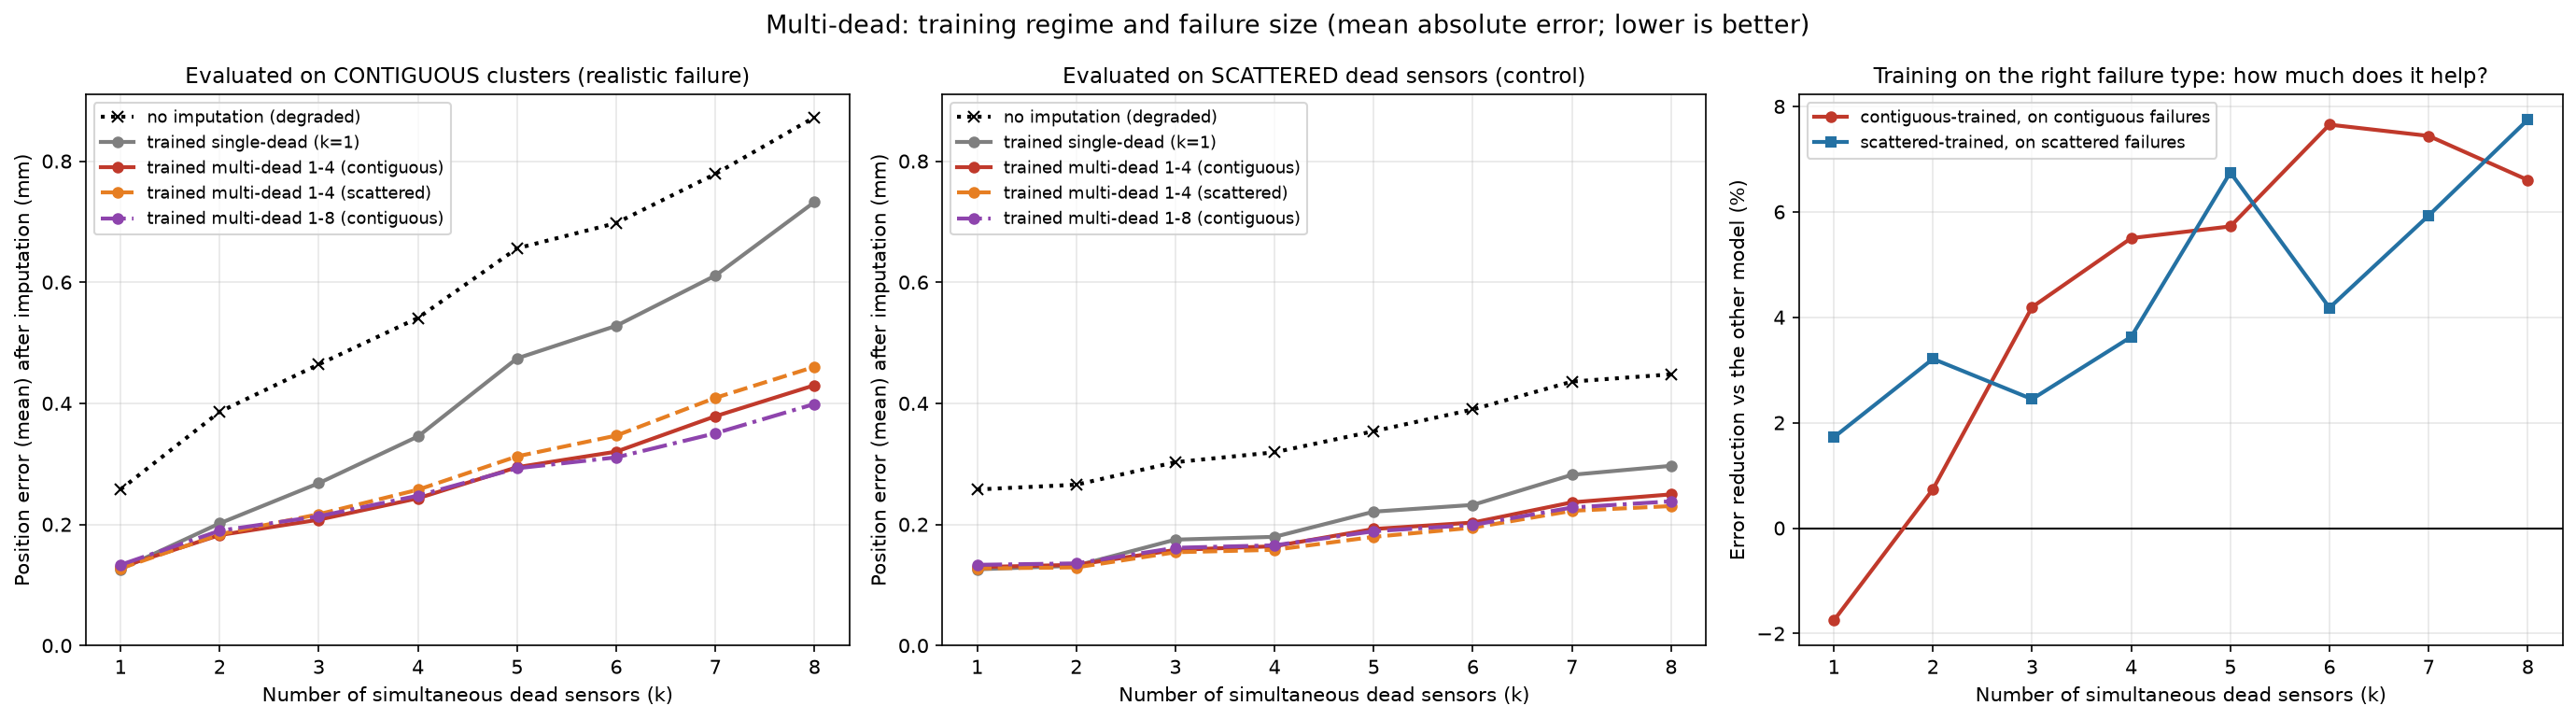
\includegraphics[width=\textwidth]{fig-multidead.png}
\caption{Error absoluto de posición tras la imputación en función del número de sensores averiados
simultáneamente, para los distintos regímenes de entrenamiento. El panel izquierdo corresponde a
fallos contiguos (caso realista) y el central a fallos dispersos (control); el panel derecho
cuantifica la ventaja de entrenar en el régimen que posteriormente se evalúa.}
\label{fig:multidead}
\end{figure}

Como referencia interpretativa, tras la imputación un fallo de ocho sensores contiguos ---el 13\,\%
del detector concentrado en una única región--- deja el módulo en una situación equivalente a la de
un fallo de dos sensores sin imputar, con un error muy inferior al paso entre sensores
(\SI{3.75}{\milli\metre}).

\subsection{Conservación del espectro de energía}
\label{subsec:res-espectro}

La Tabla~\ref{tab:res-espectro} presenta la recuperación espectral estratificada por zonas.

\begin{table}[htbp]
\centering
\caption{Recuperación espectral (\%) por zona del metahexágono y por sensor averiado,
modelo de referencia.}
\label{tab:res-espectro}
\begin{tabular}{lrrr}
\toprule
\textbf{Sensor averiado} & \textbf{Núcleo} & \textbf{Intermedia} & \textbf{Borde} \\
\midrule
$\mathrm{Ich}\,13$ (central) & 96.0 & 85.0 & 52.8 \\
$\mathrm{Ich}\,30$ (intermedio) & 78.6 & 88.7 & 91.7 \\
$\mathrm{Ich}\,32$ (mitad de lado) & 70.0 & 85.5 & 90.5 \\
$\mathrm{Ich}\,27$ (vértice) & 87.2 & 92.0 & 94.4 \\
$\mathrm{Ich}\,31$ (anómalo) & 84.3 & 70.4 & 76.5 \\
\midrule
\textbf{Media} & \textbf{83.2} & \textbf{84.3} & \textbf{81.2} \\
\bottomrule
\end{tabular}
\end{table}

La recuperación espectral se sitúa entre el 77\,\% y el 83\,\% según el sensor averiado, con un
residuo inferior al 0,5\,\% de la posición del fotopico. El resultado es \textbf{uniforme entre
zonas} (83,2 / 84,3 / 81,2), en contraste con la recuperación de posición, donde el borde sufre
apreciablemente más.

Esta disociación admite una interpretación física directa: la conservación de la energía requiere
únicamente acertar la \emph{magnitud} de la carga ausente, mientras que la reconstrucción de la
posición exige además que el \emph{reparto espacial} sea correcto. La estructura por sensor matiza
esta lectura: al enmascarar el sensor central y evaluar los eventos del borde, la recuperación cae
al 52,8\,\%, resultado esperable dado que dichos eventos apenas iluminan el centro del detector.

\subsection{Resolución espacial}
\label{subsec:res-resolucion}

La descomposición del error de posición en sesgo y dispersión arroja los resultados de la
Tabla~\ref{tab:res-resolucion}.

\begin{table}[htbp]
\centering
\caption{Descomposición del error de posición. Agregación macro sobre 61 canales.}
\label{tab:res-resolucion}
\begin{tabular}{lrrr}
\toprule
\textbf{Componente} & \textbf{Degradado} & \textbf{Imputado} & \textbf{Recuperación} \\
\midrule
Sesgo (mm) & 0.126 & 0.022 & 82.7\,\% \\
FWHM / dispersión (mm) & 0.166 & 0.085 & 48.8\,\% \\
\bottomrule
\end{tabular}
\end{table}

El contraste entre ambas componentes es informativo. El \textbf{sesgo se elimina casi por completo}
(82,7\,\%), lo que resulta esperable: el desplazamiento inducido por un canal ausente es sistemático
y por tanto predecible. La \textbf{dispersión se reduce únicamente a la mitad} (48,8\,\%), lo que
refleja el carácter irreducible de la incertidumbre evento a evento: el modelo puede estimar el
valor esperado de la carga ausente, pero no su realización concreta en un evento particular.

El análisis por canal revela que la recuperación mediana de la dispersión es del 51\,\%, con una cola
desfavorable: en dos o tres canales periféricos la mejora es marginal o incluso ligeramente negativa.

\subsection{Ensembles y descomposición sesgo-varianza}
\label{subsec:res-ensemble}

Ambos ensembles superan a la totalidad de sus miembros individuales
(Tabla~\ref{tab:res-ensemble}).

\begin{table}[htbp]
\centering
\caption{Rendimiento de los ensembles frente a la distribución de sus miembros.}
\label{tab:res-ensemble}
\begin{tabular}{lrrrr}
\toprule
\textbf{Configuración} & $\mathcal{R}_{\text{media}}$ & $\mathcal{R}_{p90}$ & \textbf{MAE} & $z$ ($\mathcal{R}_{\text{media}}$) \\
\midrule
Miembros (media $\pm$ desv.) & $52.32 \pm 0.35$ & $58.06 \pm 0.09$ & $0.6220 \pm 0.0026$ & --- \\
Ensemble homogéneo & 52.93 & 58.69 & \textbf{0.6110} & $+1.7$ \\
Ensemble heterogéneo & \textbf{53.21} & \textbf{58.73} & 0.6146 & $+2.5$ \\
\bottomrule
\end{tabular}
\end{table}

El ensemble heterogéneo supera al homogéneo en las métricas de posición, lo que establece que
\textbf{la diversidad arquitectónica aporta más que la diversidad de inicialización}. En el error de
carga, sin embargo, el homogéneo obtiene mejor resultado, lo que se atribuye a que el heterogéneo
incorpora miembros con peor rendimiento en dicha magnitud.

La lectura de mayor calado es la que corresponde a la descomposición sesgo-varianza. Si el error
estuviera dominado por la varianza entre entrenamientos, el promediado de tres modelos lo reduciría
en torno a un 40\,\%; si estuviera dominado por el límite de información, no lo alteraría. La
reducción observada es del \textbf{1,8\,\% en MAE}, de lo que se concluye que aproximadamente el
98\,\% del error es \textbf{irreducible} en el marco planteado.

\subsection{Estimación de incertidumbre}
\label{subsec:res-hetero}

El entrenamiento con la pérdida heterocedástica~\eqref{eq:nll} produjo una degradación severa:
$\mathcal{R}_{\text{media}} = 10.57$, MAE $= 1.31$ y error relativo del 63,2\,\%. La recuperación
mediana resultó \textbf{negativa} ($-18.16$), lo que indica que la imputación deja la posición en
peor situación que la ausencia de imputación.

La causa es un fallo conocido de la formulación: la pérdida~\eqref{eq:nll} permite al modelo reducir
el término cuadrático incrementando $\sigma$, pagando únicamente un coste logarítmico ---y por tanto
lineal en $\log\sigma$--- de modo que le resulta ventajoso sacrificar la precisión de $\mu$ a cambio
de declarar mayor incertidumbre. La corrección estándar consiste en un entrenamiento en dos fases,
con calentamiento bajo error cuadrático puro, o en el empleo de la formulación $\beta$-NLL. Se
documenta como línea de trabajo futuro.

\subsection{Cobertura del conjunto de entrenamiento}
\label{subsec:res-cobertura}

El experimento descrito en la Sección~\ref{subsec:exp-cobertura} arroja un resultado nítido y con
dos caras.

\begin{table}[htbp]
\centering
\caption{Efecto de entrenar con la totalidad de los módulos disponibles, a coste computacional
constante. Agregación macro sobre los 61 canales, \num{600000} eventos por fichero de test en ambos
casos.}
\label{tab:res-cobertura}
\small
\begin{tabular}{lrrr}
\toprule
\textbf{Magnitud} & \textbf{40 módulos} & \textbf{149 módulos} & \textbf{Diferencia} \\
\midrule
$\mathcal{R}_{p90}$ macro (\%) & 58.02 & 57.89 & $-0.13$ \\
$\mathcal{R}_{\text{media}}$ macro (\%) & 52.66 & 52.63 & $-0.02$ \\
$\mathcal{R}_{\text{mediana}}$ macro (\%) & 51.55 & 52.78 & $+1.23$ \\
MAE (ADC) & 0.620 & 0.616 & $-0.004$ \\
\midrule
Desviación entre canales (pts) & 4.49 & \textbf{3.77} & $-16\,\%$ \\
Recorrido entre canales (pts) & 25.2 & \textbf{15.4} & $-39\,\%$ \\
Peor canal (\%) & 38.6 & \textbf{47.9} & $\mathbf{+9.3}$ \\
Canal $\mathrm{Ich}\,31$ (\%) & 38.6 & \textbf{49.5} & $\mathbf{+11.0}$ \\
\bottomrule
\end{tabular}
\end{table}

\paragraph{En el rendimiento medio, ningún efecto.} La comparación pareada canal a canal arroja una
diferencia media de $-0.13$ puntos, con un estadístico $t = -0.49$ que no permite rechazar la
hipótesis nula, y solo 26 de los 61 canales mejoran, proporción indistinguible del azar. La
recuperación media queda en $52.63\,\%$, dentro de la banda de las réplicas
($52.32 \pm 0.35$). \textbf{El límite de rendimiento no procede de la cobertura del entrenamiento},
sino de la información físicamente disponible en los canales supervivientes. Este resultado
convierte en comprobación experimental directa lo que hasta ahora era una inferencia a partir de la
saturación de las distintas variantes arquitectónicas.

\paragraph{En la homogeneidad del detector, un efecto claro.} La dispersión entre canales se reduce
un $16\,\%$ y el recorrido entre el mejor y el peor sensor casi un $40\,\%$. El peor canal pasa de
$38.6\,\%$ a $47.9\,\%$, una mejora de $9.3$ puntos que, contrastada con la banda de las réplicas
para esa misma magnitud ($41.4 \pm 2.52$), corresponde a $z = +2.6$ y resulta por tanto
estadísticamente significativa.

\paragraph{Resolución del comportamiento anómalo de \texorpdfstring{$\mathrm{Ich}\,31$}{Ich 31}.}
Este canal, identificado sucesivamente como sensor defectuoso y como manifestación de la
variabilidad de ganancia entre módulos, mejora $11.0$ puntos al ampliar la cobertura. La
interpretación definitiva es que \textbf{los módulos de test en los que fallaba se encontraban fuera
del régimen estadístico representado en el entrenamiento}: no se trataba de un canal
intrínsecamente problemático, sino de una configuración de detector que el modelo nunca había
observado. Deja de constituir una anomalía del sensor para pasar a ser una manifestación medible de
la cobertura del conjunto de entrenamiento.

\paragraph{Conservación del espectro.} El efecto sobre la métrica energética apunta en la misma
dirección. La recuperación espectral media asciende de $82.9\,\%$ a $86.3\,\%$, y ---de nuevo lo más
relevante--- el peor caso mejora sustancialmente: la combinación más desfavorable, el canal central
evaluado sobre eventos de borde, pasa de $52.8\,\%$ a $65.8\,\%$. Nueve de las quince combinaciones
de canal y zona mejoran.

\paragraph{Resolución espacial y comparación con métodos clásicos.} Las dos magnitudes restantes se
mantienen sin cambios apreciables, lo que resulta coherente con la ausencia de efecto sobre el
rendimiento medio. La recuperación del emborronamiento mejora de forma marginal, de $48.8\,\%$ a
$49.5\,\%$, con una anchura a media altura residual prácticamente idéntica ($0.084$ frente a
$0.085$~mm) y una recuperación del sesgo equivalente ($82.6\,\%$ frente a $82.7\,\%$). La ventaja
sobre la regresión lineal, que sustenta la necesidad del aprendizaje profundo, se conserva en
$11.3$ puntos frente a los $11.5$ del modelo de referencia; la diferencia queda holgadamente dentro
de la variabilidad entre entrenamientos. Ninguno de los dos observables se ve por tanto perjudicado
por la ampliación de la cobertura.

\paragraph{Contrapartida: pérdida de robustez ante fallos múltiples.} La evaluación multi-dead
revela, sin embargo, un efecto de signo contrario que obliga a matizar la valoración. Ambos modelos
se entrenaron exclusivamente con un canal enmascarado, de modo que un fallo de dos o más sensores
constituye para ellos una situación no observada durante el entrenamiento. Con un único canal
averiado, el modelo de cobertura completa es superior, y de forma marcada en el peor caso
($45.9\,\%$ frente a $34.7\,\%$). Pero al aumentar el tamaño del fallo su rendimiento
\textbf{se desploma}: en agrupaciones contiguas de dos sensores la recuperación media cae a valores
negativos ---esto es, la imputación empeora la posición respecto a no imputar--- mientras que el
modelo de referencia se degrada de forma suave y conserva un $49.3\,\%$.

\begin{table}[htbp]
\centering
\caption{Recuperación media (\%) frente al tamaño del fallo, para dos modelos entrenados ambos con
un solo canal enmascarado. Valores negativos indican que la imputación desplaza la posición más de
lo que lo hace el propio fallo.}
\label{tab:res-cobertura-multidead}
\small
\begin{tabular}{lrrrr}
\toprule
\textbf{Modelo} & $k=1$ & $k=2$ & $k=3$ & $k=4$ \\
\midrule
\multicolumn{5}{l}{\emph{Agrupación contigua}} \\
\quad 40 módulos (referencia) & 51.39 & \textbf{49.28} & \textbf{44.21} & \textbf{37.59} \\
\quad 149 módulos & \textbf{51.64} & $-27.35$ & $-123.65$ & $-161.83$ \\
\midrule
\multicolumn{5}{l}{\emph{Fallo disperso}} \\
\quad 40 módulos (referencia) & 51.39 & \textbf{50.71} & \textbf{43.19} & \textbf{43.37} \\
\quad 149 módulos & \textbf{51.64} & 45.13 & 13.62 & $-3.96$ \\
\bottomrule
\end{tabular}
\end{table}

La interpretación más plausible es que el entrenamiento prolongado sobre un régimen de fallo único
---149 épocas frente a 40, con el punto de control seleccionado en la época 133--- produce una
función más ajustada a esa condición concreta y, por ello, más frágil fuera de la distribución de
entrenamiento. La cobertura completa mejora el caso para el que el modelo fue entrenado a costa de
su capacidad de extrapolación.

\paragraph{Implicación práctica.} Ampliar la cobertura no mejora el rendimiento promedio, pero
\textbf{homogeneiza la respuesta del detector sin coste computacional adicional}: eleva el peor
sensor nueve puntos y mejora la conservación del espectro. En un dispositivo real, donde la garantía
relevante es que ningún sensor se degrade de forma catastrófica, ese comportamiento resulta
preferible a una mejora marginal de la media. Ahora bien, la pérdida de robustez ante fallos
múltiples impide recomendar su adopción sin más: un modelo de producción con cobertura completa
debería entrenarse necesariamente en régimen multi-dead
(Sección~\ref{subsec:exp-multidead}), combinando ambas mejoras en lugar de intercambiarlas.

\subsection{Detección de canales defectuosos}
\label{subsec:res-bad}

La Tabla~\ref{tab:res-bad-roc} recoge la validación del estadístico de detección mediante inyección
de fallos con verdad conocida.

\begin{table}[htbp]
\centering
\caption{Validación del detector de canales defectuosos. Área bajo la curva ROC y tasas de
detección en el punto de operación.}
\label{tab:res-bad-roc}
\begin{tabular}{lrrr}
\toprule
\textbf{Severidad del fallo} & \textbf{AUC} & \textbf{TPR} ($Z=2.5$) & \textbf{FPR} \\
\midrule
100\,\% (canal muerto) & 1.000 & 1.000 & 0.009 \\
70\,\% & 0.998 & 0.952 & 0.009 \\
50\,\% & 0.973 & 0.422 & 0.009 \\
30\,\% & 0.868 & 0.091 & 0.009 \\
\bottomrule
\end{tabular}
\end{table}

El estadístico identifica los canales completamente inactivos con separación perfecta
($\mathrm{AUC} = 1.000$) y mantiene un rendimiento elevado para degradaciones severas. La tasa de
falsos positivos en los canales de borde resulta equivalente a la de los canales centrales, lo que
confirma que la normalización por canal resuelve efectivamente el problema del gradiente
estructural.

Las degradaciones moderadas, en cambio, no resultan separables en el punto de operación: si bien el
área bajo la curva indica que la información está presente, explotarla exigiría reducir el umbral y
asumir una tasa de falsos positivos considerablemente mayor.

\begin{figure}[htbp]
\centering
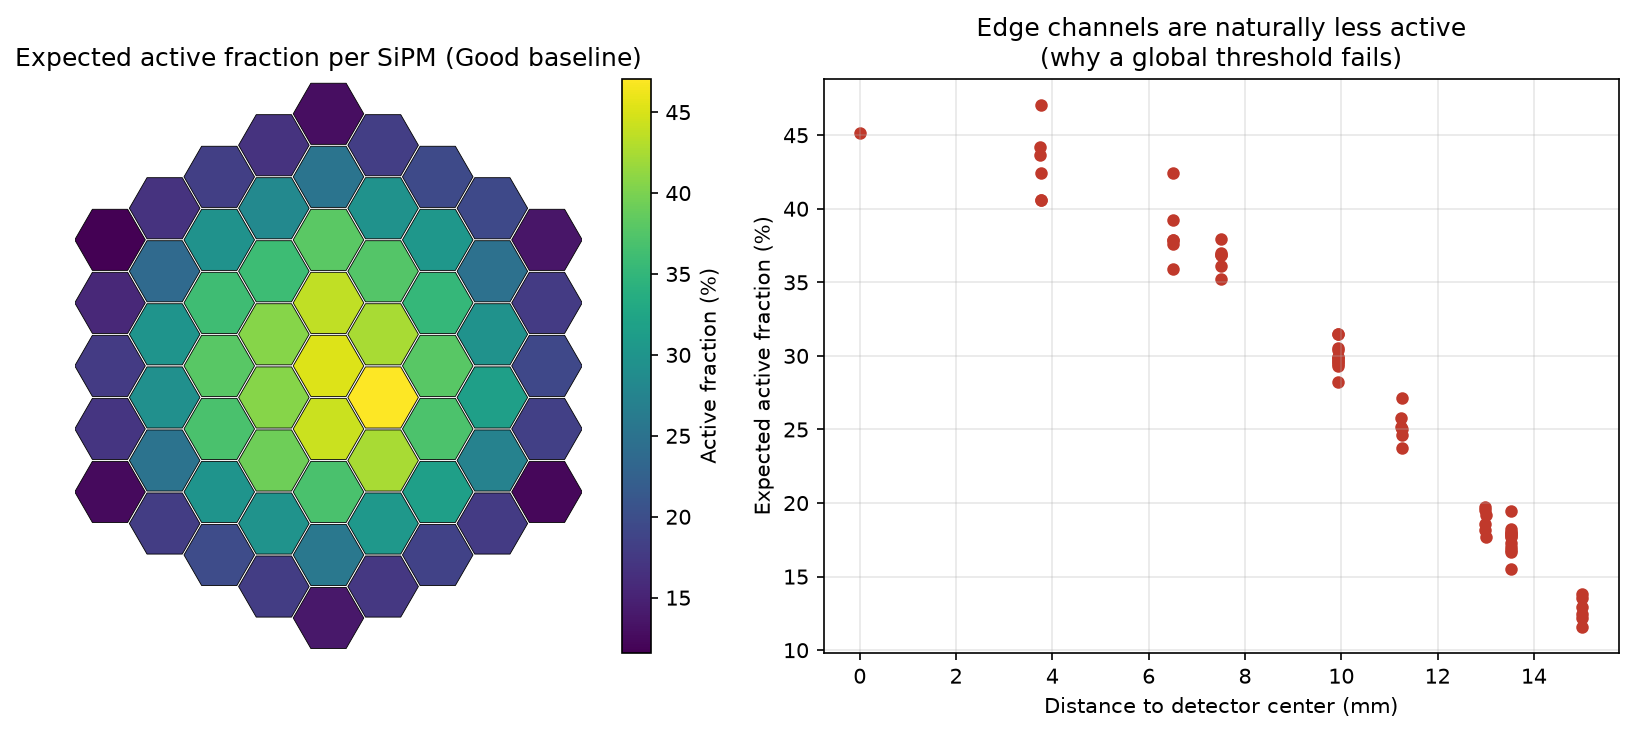
\includegraphics[width=0.95\textwidth]{fig-baseline-bad.png}
\caption{Actividad esperada por sensor en módulos sanos. Izquierda: mapa hexagonal del detector.
Derecha: dependencia con la distancia al centro, con una correlación de $-0.97$. Este gradiente
estructural es la razón por la que un umbral de detección global resulta inadecuado.}
\label{fig:baseline-bad}
\end{figure}

\begin{figure}[htbp]
\centering
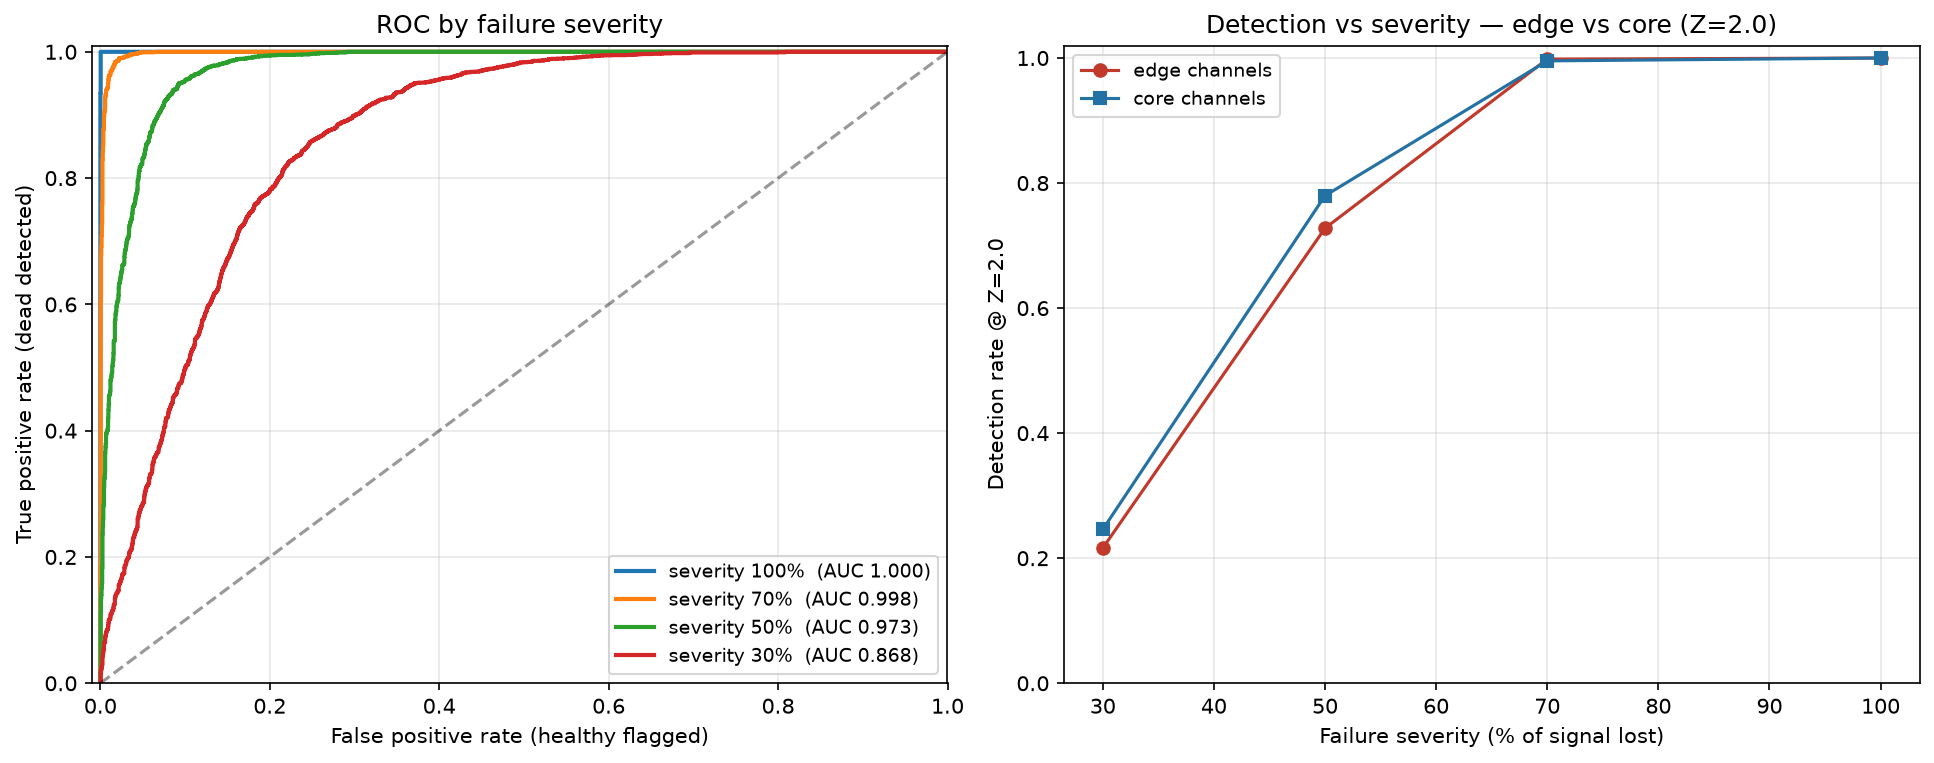
\includegraphics[width=0.95\textwidth]{fig-roc-bad.png}
\caption{Validación del estadístico de detección mediante inyección de fallos con verdad conocida.
Izquierda: curvas ROC para distintas severidades. Derecha: tasa de detección en el punto de
operación, desglosada entre canales de borde y centrales.}
\label{fig:roc-bad}
\end{figure}

Aplicado a los 62 módulos \textsc{Bad} con normalización por módulo y umbral $Z = 2.0$, el
procedimiento identifica canales defectuosos en \textbf{48} de los 62 módulos, marcando
\textbf{278} canales en total, y señala \textbf{12} módulos como globalmente desplazados.



\begin{figure}[htbp]
\centering
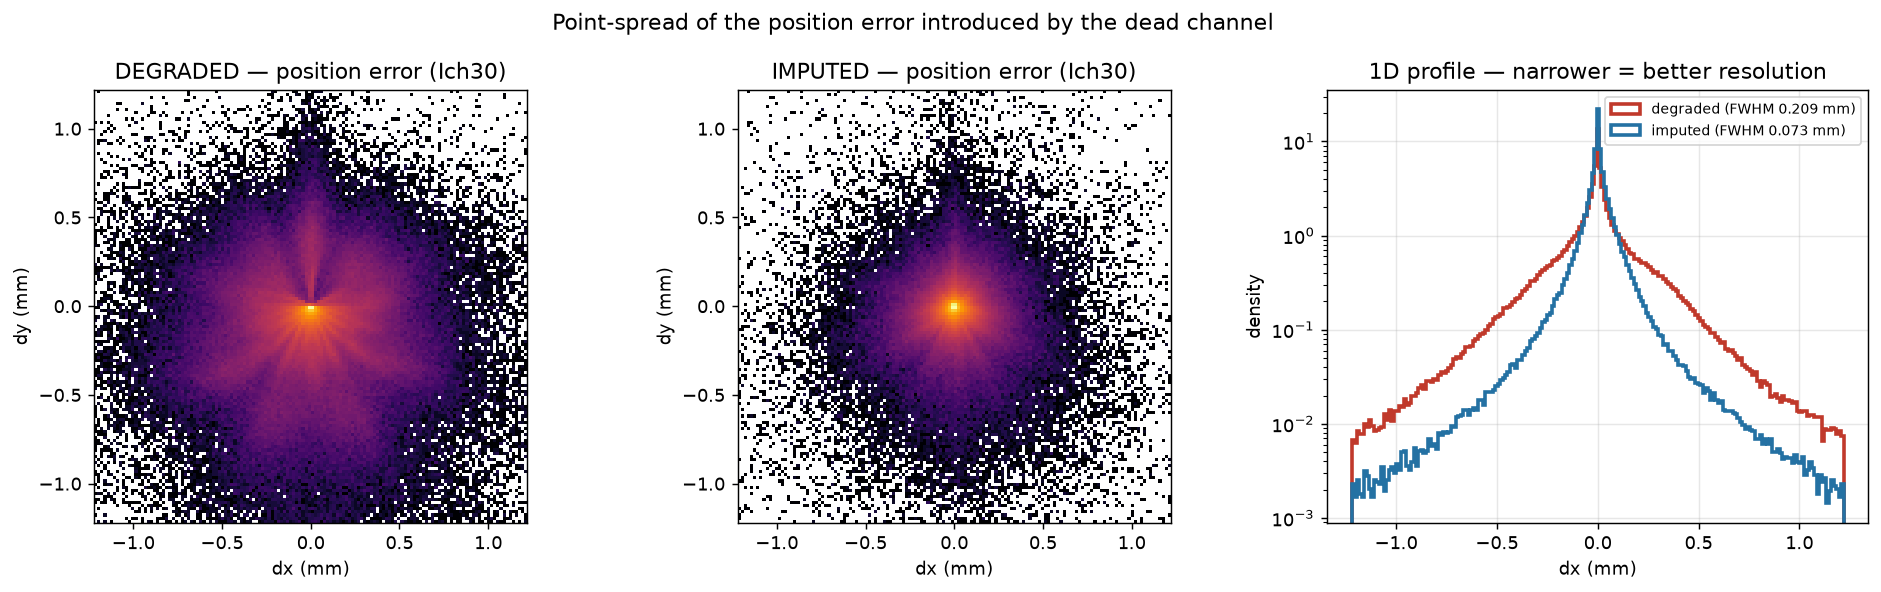
\includegraphics[width=0.95\textwidth]{fig-pointspread.png}
\caption{Distribución bidimensional del error de posición (\emph{point spread}) para el canal
$\mathrm{Ich}\,30$, antes y después de la imputación. La nube de la derecha es simultáneamente más
estrecha (menor dispersión) y está mejor centrada (menor sesgo) que la de la izquierda.}
\label{fig:pointspread}
\end{figure}

\begin{figure}[htbp]
\centering
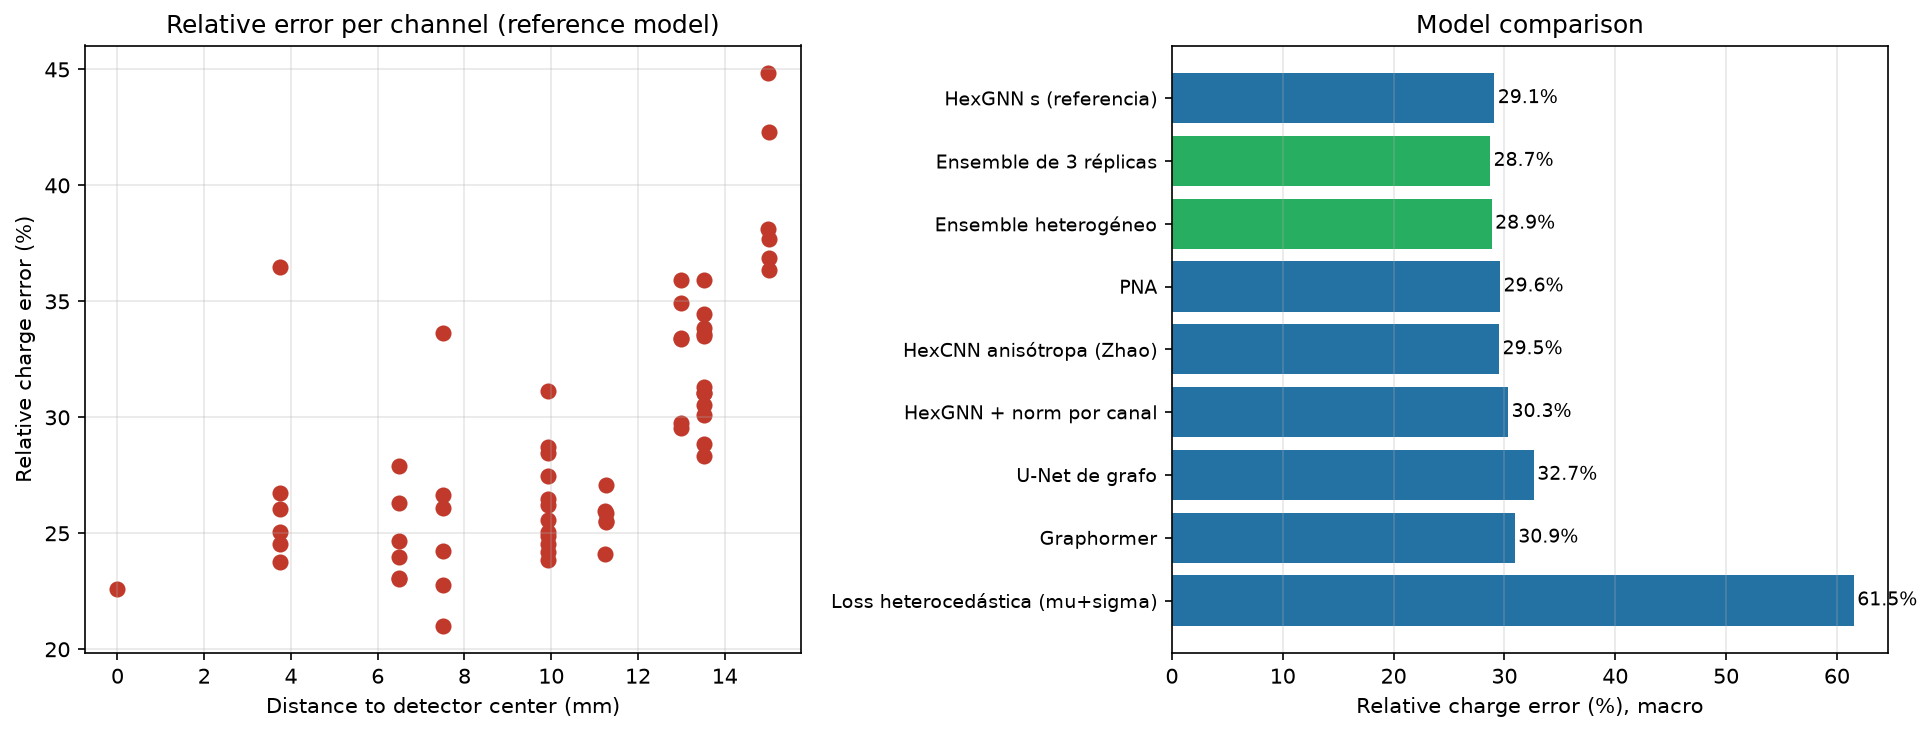
\includegraphics[width=0.95\textwidth]{fig-error-relativo.png}
\caption{Error relativo de carga. Izquierda: valor por canal frente a la distancia al centro del
detector, que evidencia el gradiente centro--borde. Derecha: comparación agregada entre las
configuraciones evaluadas.}
\label{fig:error-relativo}
\end{figure}

\section{Discusión}
\label{sec:discusion}

\subsection{Sobre la naturaleza del límite de rendimiento}

El conjunto de resultados converge de forma consistente hacia una conclusión: el rendimiento
alcanzado no está limitado por la arquitectura ni por la capacidad del modelo, sino por la
\textbf{información físicamente disponible} en los sensores operativos.

Esta conclusión se sustenta en cuatro evidencias independientes. En primer lugar, el incremento de
capacidad no mejora el rendimiento, e incluso lo degrada. En segundo lugar, diez variantes
arquitectónicas ---incluyendo transformadores, arquitecturas multiescala, agregadores múltiples y la
convolución hexagonal canónica--- no superan a la configuración de referencia. En tercer lugar, el
análisis por anillos demuestra que la información explotable se agota en el segundo anillo de
vecindad. Y en cuarto lugar, el ensemble ---que cancela la varianza entre entrenamientos--- recupera
únicamente un 1,8\,\% del error, lo que sitúa en torno al 98\,\% la fracción irreducible.

La descomposición del error de posición en sesgo y dispersión ofrece la interpretación física de
este límite. El sesgo, sistemático y por tanto predecible, se elimina casi por completo. La
dispersión, que corresponde a la incertidumbre sobre la realización concreta de la carga en cada
evento individual, solo se reduce a la mitad. Ninguna arquitectura puede eliminar esta segunda
componente, pues la información necesaria simplemente no está presente en los datos observados.

\subsection{Sobre la adecuación del diseño arquitectónico}

Los resultados permiten justificar el diseño adoptado desde tres perspectivas independientes.

La comparación con métodos clásicos establece que el aprendizaje profundo es \textbf{necesario}: la
red supera en 11,5 puntos a la regresión lineal. El análisis por anillos establece que la
información es \textbf{local}. Y la ablación del grafo establece que el prior geométrico es
\textbf{determinante}. En conjunto, estas tres evidencias caracterizan el modelo adecuado como uno
que sea simultáneamente local, no lineal e informado por la geometría del detector, que es
precisamente la descripción de la arquitectura propuesta.

El análisis de equivarianza añade una cuarta propiedad: la isotropía. La arquitectura respeta por
construcción la simetría $D_6$ del detector, propiedad que las variantes anisótropas rompen sin
obtener contrapartida, dado que el transporte de luz en el cristal es radialmente simétrico.

\subsection{Fortalezas del trabajo}

Cabe destacar como fortalezas metodológicas la definición de un marco de evaluación con significado
físico, que trasciende el error de reconstrucción y cuantifica el impacto sobre posición, energía y
resolución; el diseño diferencial emparejado para la evaluación espectral, que elimina la necesidad
de calibración previa; la estratificación mediante el metahexágono, físicamente motivada por la
geometría del absorbente; la inclusión sistemática de controles ---ablación del grafo, régimen
disperso, control de ruido en $k=1$, réplicas independientes--- que permiten atribuir causalmente los
efectos observados; y la cuantificación explícita de la variabilidad entre entrenamientos, que
proporciona el criterio para juzgar la significación de las comparaciones.

En el plano de los resultados, el hallazgo de que entrenar con fallos múltiples confiere robustez
sin coste alguno en el caso de un único canal tiene aplicabilidad práctica directa.

\subsection{Limitaciones}

\paragraph{Estadística de módulos reducida.} Conviene distinguir esta limitación de la cobertura del
entrenamiento tratada más abajo, con la que resulta fácil confundirla: aquella se refiere a
\emph{cuántos detectores ve el modelo} y afecta a lo que aprende; ésta se refiere a \emph{cuántos
detectores se emplean para medirlo} y afecta a la precisión de la métrica. Son independientes, y el
experimento de cobertura no resuelve la segunda.

La partición reserva únicamente cinco módulos para test. Aunque la estadística de eventos es holgada
---del orden de tres millones---, la de \emph{detectores} es pobre, de modo que las conclusiones
referidas a canales individuales pueden reflejar particularidades de esos cinco módulos concretos.
El caso del canal $\mathrm{Ich}\,31$ ilustra el problema: identificado inicialmente como canal
sistemáticamente anómalo, el análisis posterior reveló que su comportamiento en los módulos de
entrenamiento es normal y que la anomalía se concentra en dos módulos asignados a test; el
experimento de cobertura confirmó después que dichos módulos quedaban fuera del régimen estadístico
representado durante el entrenamiento.

La consecuencia metodológica es que las métricas agregadas carecen de una barra de error asociada al
\emph{efecto de módulo}: se dispone de la variabilidad entre entrenamientos
(Sección~\ref{subsec:res-replicas}), pero no de la variabilidad entre detectores. El procedimiento
descrito en el párrafo anterior ---evaluar sobre los 119 módulos no observados--- permite estimarla
sin reentrenar y se identifica como la comprobación pendiente de mayor valor.

\paragraph{Ausencia de validación cruzada.} No se ha realizado validación cruzada por módulos. La
razón no es el coste ---repetir el entrenamiento cinco veces es perfectamente asumible--- sino que
el número de hiperparámetros a ajustar es reducido y la selección del punto de control ya descansa
en un conjunto de validación independiente. Conviene, no obstante, precisar qué quedaría por
resolver: la validación cruzada no se necesitaría aquí para \emph{ajustar} nada, sino para
\textbf{acotar la sensibilidad de las métricas a qué cinco módulos concretos quedaron reservados
para test}, que es una cuestión distinta y sí pertinente.

Existe, además, una alternativa más económica y estadísticamente más potente que la validación
cruzada para esa pregunta concreta, derivada de la propia mecánica de rotación de ficheros. Puesto
que un modelo de 40 épocas solo llega a ver 40 de los 149 módulos de entrenamiento, los 109
restantes ---junto a los 5 de validación y los 5 de test--- constituyen \textbf{119 módulos que el
modelo no ha observado nunca}. Evaluar sobre ellos proporciona la dispersión entre detectores con
una estadística veinticuatro veces mayor que la del conjunto de test, y sin reentrenar. Es el
procedimiento recomendado para cerrar la limitación descrita en el párrafo siguiente.

\paragraph{Cobertura parcial del conjunto de entrenamiento.} El presupuesto de 40 épocas, combinado
con una rotación cíclica sobre la lista ordenada de ficheros, hace que el modelo utilice 40 de los
149 módulos disponibles, y que sean siempre los mismos. Como se detalla en la
Sección~\ref{subsec:carga-entrenamiento}, ese subconjunto resulta además más homogéneo que la
población completa. El experimento de la Sección~\ref{subsec:res-cobertura} demuestra que esta
limitación \textbf{no afecta al rendimiento medio} ---y por tanto no compromete ninguna de las
comparaciones entre modelos---, pero sí a la \emph{homogeneidad} entre canales: el protocolo de
producción subestima el peor caso en unos nueve puntos. Para trabajo posterior se recomienda adoptar
la cobertura completa, que no conlleva coste adicional.

\paragraph{Ausencia de calibración y filtrado en energía.} El conjunto incluye eventos Compton y de
fondo sin calibración de ganancia. Aunque el diseño diferencial cancela estos efectos en la
evaluación espectral, no puede descartarse que un conjunto calibrado y filtrado permitiera un
rendimiento superior.

\paragraph{Criterio de selección de modelo.} La métrica empleada para seleccionar el punto de
control no rastrea perfectamente el rendimiento en test, como se comprobó en el banco de pruebas.

\paragraph{Alcance del detector de canales defectuosos.} El estadístico desarrollado identifica de
forma fiable los canales inactivos, pero no separa las degradaciones moderadas de la variabilidad
normal, ni detecta canales con ganancia anómalamente elevada, dado que el estadístico es de una sola
cola. La distribución de puntuaciones en los módulos reales no presenta bimodalidad clara, lo que
indica que ``canal defectuoso'' no constituye una categoría con una firma estadística única sino un
conjunto heterogéneo de modos de fallo.

\paragraph{Ausencia de verdad de referencia en los módulos averiados.} La validación del detector se
apoya en fallos inyectados sobre módulos sanos, lo que garantiza una verdad conocida a costa de
evaluar un modo de fallo idealizado. En los módulos defectuosos reales no se dispone de anotación,
de modo que las detecciones no pueden contrastarse y el rendimiento medido no es directamente
extrapolable. La herramienta de etiquetado manual descrita en la Sección~\ref{subsec:exp-bad} se ha
desarrollado precisamente para levantar esta limitación; la anotación de los módulos y la medida del
acuerdo con el estadístico automático constituyen trabajo en curso.

\paragraph{Coste de inferencia del ensemble.} La mejor configuración identificada triplica el coste
de inferencia. Constituye por tanto una mejora en recursos y no en método, extremo que debe
explicitarse al reportar el resultado.

\subsection{Comparación entre aproximaciones}

La comparación entre familias arquitectónicas resulta ilustrativa. Los métodos sin estructura (MLP)
alcanzan recuperaciones del 48--51\,\%. Las arquitecturas basadas en paso de mensajes local se sitúan
en el rango 55--58\,\%. Las basadas en atención global obtienen 54--55\,\%, es decir, peor que las
locales pese a disponer de hasta cien veces más parámetros. La ordenación es coherente con la
naturaleza del problema: la estructura de grafo aporta, mientras que el contexto global no
únicamente no aporta sino que diluye la señal local relevante.

En cuanto a las estrategias de mejora ajenas a la arquitectura, se observa una asimetría notable:
mientras que ninguna modificación arquitectónica superó la referencia, el promediado de modelos sí
produjo una mejora estadísticamente significativa, aunque de magnitud modesta. Esto refuerza la
interpretación de que el margen de mejora disponible no reside en el diseño del modelo.


\section{Conclusiones preliminares}
\label{sec:conclusiones}

\subsection{Respuesta a los objetivos planteados}

\textbf{Sobre el diseño del modelo y el prior geométrico.} Se ha desarrollado una red neuronal de
grafos que explota la adyacencia física de los sensores, alcanzando una recuperación del error de
posición del 52--58\,\% con únicamente \num{38305} parámetros. La ablación del grafo establece de
forma concluyente que dicho prior es el elemento determinante del rendimiento: su eliminación reduce
la recuperación a la mitad.

\textbf{Sobre el marco de evaluación física.} Se ha desarrollado un conjunto de métricas que
cuantifican el impacto de la imputación sobre las tres magnitudes de interés. Los resultados indican
que el método recupera el 52--58\,\% del error de posición, el 77--83\,\% de la conservación del
espectro y el 48,8\,\% de la dispersión espacial, eliminando además el 82,7\,\% del sesgo
sistemático.

\textbf{Sobre la justificación del aprendizaje profundo.} La comparación con métodos clásicos
establece una ventaja de 11,5 puntos frente a la regresión lineal. El análisis por anillos precisa
el origen de dicha ventaja: no procede del acceso a información global ---que resulta irrelevante
más allá del segundo anillo--- sino de la capacidad de modelar relaciones no lineales.

\textbf{Sobre el límite del rendimiento.} El conjunto de evidencias establece que el rendimiento
está limitado por la información disponible y no por el modelo. La formulación de este resultado es
en sí misma una aportación: no se trata de que no se hayan encontrado arquitecturas mejores, sino de
que se ha caracterizado por qué la arquitectura adoptada es la adecuada.

\textbf{Sobre los fallos múltiples.} Entrenar con fallos múltiples contiguos reduce a la mitad el
error con ocho canales averiados, sin penalización alguna en el caso de un único canal, y
generalizando por encima del rango de entrenamiento. El régimen espacial del entrenamiento resulta
relevante, con una ventaja del 6--8\,\% frente a un nivel de ruido del 1,8\,\%.

\textbf{Sobre la detección de canales defectuosos.} Se ha desarrollado un estadístico que identifica
con separación perfecta los canales inactivos, resolviendo el problema del gradiente estructural
centro-borde. Su alcance queda limitado a los fallos severos.

\subsection{Contraste de las hipótesis planteadas}

De las hipótesis formuladas, se confirmaron la relativa al prior geométrico, la relativa a la
localidad de la información, la relativa al mayor daño de los fallos contiguos y la relativa al papel
del ensemble como estimador de la componente reducible del error.

Se refutaron, en cambio, las hipótesis relativas a la utilidad de las pérdidas physics-informed, al
beneficio de incorporar información direccional, a la ventaja de las arquitecturas de mayor
capacidad y a la conveniencia de la normalización por canal. Esta última merece comentario: la
hipótesis predecía una mejora en los canales periféricos, y el resultado fue una degradación
concentrada en los canales centrales. La explicación es que el estimador de posición pondera las
cargas cuadráticamente, de modo que los canales más brillantes dominan la magnitud de interés; la
pérdida cuadrática sin equalizar estaba, de forma no premeditada, alineada con esa ponderación, y
equalizar los canales rompe dicha alineación.

\subsection{Líneas de trabajo futuro}

Se identifican las siguientes líneas de continuación:

\begin{enumerate}
    \item \textbf{Estimación de incertidumbre con formulación corregida}, empleando entrenamiento en
    dos fases o la formulación $\beta$-NLL, con la finalidad de identificar y descartar los eventos
    cuya imputación resulte poco fiable.

    \item \textbf{Ampliación del estadístico de detección} mediante observables sensibles a la forma
    de la distribución de carga y con formulación de dos colas, que permitiría abordar los modos de
    fallo actualmente no cubiertos.

    \item \textbf{Combinación de cobertura completa y entrenamiento multi-canal.} Los resultados de
    la Sección~\ref{subsec:res-cobertura} muestran que ampliar la cobertura de módulos mejora la
    homogeneidad entre sensores y la conservación del espectro, pero degrada la extrapolación a
    fallos múltiples, mientras que el entrenamiento en régimen multi-canal
    (Sección~\ref{subsec:res-multidead}) proporciona precisamente esa robustez sin coste apreciable
    en el caso de fallo único. Al actuar sobre aspectos independientes del procedimiento, ambas
    intervenciones son en principio acumulables, y su combinación constituye la vía más directa
    hacia un modelo de producción que reúna las dos propiedades.

    \item \textbf{Anotación manual completa de los módulos averiados} con la herramienta descrita en
    la Sección~\ref{subsec:exp-bad}, que proporcionaría la verdad de referencia necesaria para medir
    el acuerdo entre el criterio experto y el estadístico automático sobre datos reales, y no
    únicamente sobre fallos inyectados.

    \item \textbf{Validación cruzada por módulos}, que permitiría acotar la sensibilidad de los
    resultados a la partición concreta y robustecer las conclusiones referidas a canales
    individuales.

    \item \textbf{Incorporación de la calibración en energía} y del filtrado correspondiente, con el
    fin de determinar si un conjunto de datos calibrado permite superar el límite observado.

    \item \textbf{Extensión a la corrección de canales anómalos}, generalizando el planteamiento
    desde la imputación de canales ausentes a la corrección de canales con respuesta alterada.

    \item \textbf{Evaluación del impacto sobre la imagen reconstruida}, cerrando la cadena desde la
    recuperación del módulo individual hasta la calidad de la imagen tomográfica final.
\end{enumerate}

% =====================================================================
%  MARCADORES PENDIENTES DE COMPLETAR
% =====================================================================
% TODO(1): Especificar el modelo concreto de SiPM, sus dimensiones activas y el
%          espesor del cristal LYSO. Esta información debe obtenerse de la
%          documentación del sistema experimental o del equipo del laboratorio.
% TODO(2): Detallar la actividad de la fuente de 22Na, la geometría de irradiación
%          y la duración de las adquisiciones.
% TODO(3): Especificar el modelo de ASIC empleado y el valor del umbral de
%          discriminación aplicado.
% TODO(5): Incluir las referencias bibliográficas correspondientes a: GraphSAGE
%          (Hamilton et al., 2017), PNA (Corso et al., 2020), Graphormer (Ying
%          et al., 2021), Graph U-Net (Gao y Ji, 2019), convolución hexagonal
%          (Zhao et al., 2021), beta-NLL (Seitzer et al., 2022), AdamW (Loshchilov
%          y Hutter, 2019) y modified z-score (Iglewicz y Hoaglin, 1993).
% TODO(6): Generar y enlazar las figuras marcadas como [FIGURA SUGERIDA].

\end{document}
